\documentclass[a4paper, 11pt, UTF8]{article}
\usepackage{amssymb,amsmath,amsfonts}
\usepackage{ctex}
\usepackage{setspace}
\usepackage{graphicx}
\usepackage{hyperref}
\usepackage{fontspec}
\usepackage{unicode-math}
\usepackage{ulem}
\usepackage{color}
\usepackage{tabularx}
\usepackage{xargs}
\usepackage[left=1cm,right=1cm,top=1cm,bottom=0cm]{geometry}

\hypersetup{colorlinks=true,linkcolor=blue,urlcolor=cyan}

\begin{document}
\begin{large}
\parindent 0pt

%{ 关于字体设置
\setmainfont{TeXGyrePagella-Regular}
\setmathfont{TeXGyrePagellaMath-Regular}
\setmathfont[range={\mathcal,\Longleftrightarrow,\Longrightarrow,\Longleftarrow,\Rightarrow,\Leftarrow,\Leftrightarrow}]{LatinModernMath-Regular}
\setmathfont[range={\backslash}]{MathJax_Size1-Regular.otf}
\setmathfont[range={\mathbb}]{TeXGyreSchola-Regular}
\setmathfont[range={\complement}]{TeXGyrePagella-Bold}
\setmathfont[range=\mathfrak]{TeXGyrePagella-Regular}
\setmathfont[range={\tilde}]{DejaVuMathTeXGyre.ttf}


\newfontfamily{\tgnr}{TeXGyrePagella-Regular}
\newfontfamily{\tgbf}{TeXGyreSchola-Regular}
\newfontfamily{\tgbfx}{TeXGyrePagella-Bold}
\newfontfamily{\tgbfxx}{timesbd.ttf}
\newfontfamily{\tgsl}{TeXGyrePagella-Italic}
\newfontfamily{\tgsc}{TeXGyrePagella-BoldItalic}
\newfontfamily{\forbra}{MathJax_Size1-Regular.otf}
\newfontfamily{\forbrax}{MathJax_Size2-Regular.otf}

\newcommand{\Largenr}[1]{{\Large\tgnr#1}}
\newcommand{\Largesl}[1]{{\Large\tgsl#1}}
\newcommand{\Largebf}[1]{{\Large\tgbf#1}}
\newcommand{\Largebfx}[1]{{\Large\tgbfx#1}}
\newcommand{\Largebfxx}[1]{{\Large\tgbfxx#1}}

\def\envFontLarge{\def\envFontA{\LARGE}\def\envFont{\Large}\def\envFontB{\large}}
\def\envFontDefault{\def\envFontA{\Large}\def\envFont{\large}\def\envFontB{\normalsize}}
\newcommand{\envFontSmall}[1][\small]{\def\envFontA{\Large}\def\envFont{\normalsize}\def\envFontB{#1}}
\newcommand{\TextE}[1]{\dbsp\envFontLarge\Largesl{#1}\envFontDefault\par\IndentE}
\newcommand{\TextN}[1]{\dbsp\envFontLarge\Largesl{#1}\envFontDefault\par\IndentN}
\newcommand{\TextB}[1]{\dbsp\envFontLarge\Largesl{#1}\envFontDefault\par\IndentB}
\newcommand{\TextNL}[1]{\dbsp\envFontLarge\Largesl{#1}\envFontDefault\par\IndentNL}
%}

%{ 关于排版缩进的便捷指令
%  · {题目内容}\par\IndentB
%  8 {题目内容}\par\IndentN
% 19 {题目内容}\par\IndentNL
% EXAMPLE: {text}\par\IndentE
\def\IndentB{\Blind{\BulletPoint }}
\def\IndentN{\hspace{8.7pt}}
\def\IndentNL{\hspace{16pt}}
\def\IndentE{{\large\Blind{{\BulletPoint} {\Example}\,\,\,}}}

% 用于对齐(a)(b)(c)(d)
%(a) {text} \par\quad\Ha
%... \par\quad\Ha
%{text} \par\quad
%(b) {text} \par\quad\Hb
%... \par\quad\Ha
%{text} \par\quad
%(c) {text} \par\quad\Hc
%... \par\quad\Ha
%{text} \par\quad
%(d) {text} \par\quad\Hd
%... \par\quad\Ha
%{text} \par\quad
\def\Ha{{\large\Blind{(a) }}}
\def\Hb{{\large\Blind{(b) }}}
\def\Hc{{\large\Blind{(c) }}}
\def\Hd{{\large\Blind{(d) }}}

% 用于对齐(i)(ii)(iii)
%(i) {text} \par\quad\Hi
%... \par\quad\Hi
%{text} \par\quad\Endi
%(ii)  {text} \par\quad\Hii
%... \par\quad\Hii
%{text} \par\quad\Endii
%(iii) {text} \par\quad\Hiii
%... \par\quad\Hiii
%{\text}\par\quad
\def\Endi{}
\def\Endii{}
\def\Hi{\Blind{(i) }}
\def\Hii{\Blind{(ii) }}
\def\Hiii{}

% 用于对齐(I)(II)(III)
\def\EndI{}
\def\EndII{}
\def\EndIII{}
\def\HI{\Blind{(I) }}
\def\HII{\Blind{(II) }}
\def\HIII{\Blind{(III) }}
%}

%{ 关于文本环境
\newcommand{\hMath}[5][-4pt]{#3\hspace{#1}\begin{array}{#2}#5\end{array}\hspace{#1}#4}
\newcommand{\MathLeftBrace}				[2]{\hMath[0pt]{#1}{\left\{}{\right.}{#2}}
\newcommand{\MathRightBrace}			[2]{\hMath[0pt]{#1}{\left.}{\right\}}{#2}}
\newcommand{\MathLeftrightBrace}		[2]{\hMath[0pt]{#1}{\left\{}{\right\}}{#2}}
\newcommand{\MathLeftMid}				[2]{\hMath[0pt]{#1}{\left|}{\right.}{#2}}
\newcommand{\MathRightMid}				[2]{\hMath[0pt]{#1}{\left.}{\right|}{#2}}
\newcommand{\MathLeftrightMid}			[2]{\hMath[0pt]{#1}{\left|}{\right|}{#2}}
\newcommand{\MathLeftrightPare}			[2]{\hMath[0pt]{#1}{\left(}{\right)}{#2}}

\newcommand{\hText}[4][-4pt]{\hMath[#1]{c}{#2}{#3}{#4}}
\newcommand{\Par}[2][-5pt]{{\text{\forbra\envFontB(\hspace{1pt}}}#2{\text{\hspace{1pt}\forbra\envFontB)}}}%{\hText[-4pt]{}{}{$\hspace{-1pt}{\envFontB$\hText[#1]{\left(}{\right)}{${\envFont$#2$}$}$}$}}
\newcommand{\Mid}[2][-3pt]{\hText[#1]{\left|}{\right|}{#2}}%{\hText[-2pt]{}{}{$\hspace{-1pt}{\envFontB$\hText[#1]{\left|}{\right|}{${\envFont$#2$}$}$}$}}
\newcommand{\Bra}[2][-5pt]{{\text{\forbra\envFont{\{}}}#2{\text{\forbra\envFont\}}}}%{\hText[-4pt]{}{}{$\hspace{-1pt}{\envFontB$\hText[#1]{\left\{}{\right\}}{${\envFont$#2$}$}$}$}}
\newcommand{\SmallPar}[1]{\text{(}#1\text{)}}
\newcommand{\BigPar}[1]{{\text{\envFont\forbra(\hspace{1pt}}}#1{\text{\hspace{1pt}\envFont\forbra)}}}
\newcommand{\XPar}[1]{{\text{\envFont\forbrax(\hspace{1pt}}}#1{\text{\hspace{1pt}\envFont\forbrax)}}}
\newcommand{\Sbra}[1]{{\text{\envFont\forbra[\hspace{1pt}}}#1{\text{\envFont\forbra\hspace{1pt}]}}}
\newcommand{\XSbra}[1]{{\text{\envFont\forbrax[}}#1{\text{\envFont\forbrax]}}}
\newcommand{\zeroSubs}[1][\Bra]{{#1{0}}}

\newcommand{\ExampleX}[2][\Solution]{
	{\BulletPoint} {\Example}\,\,\,{#2}\envFontDefault\vspace{-16pt}\par
	#1
}
\newcommand{\ProblemN}[3][\Solution]{
	{\Onumber{#2}} {#3}\envFontDefault\vspace{-16pt}\par
	#1
}
\newcommandx{\ProblemNor}[5][1=\Solution,4=\Sbra]{
	{\Onumber{#2}} {\dbsp#4{\OR({\normalsize#3})}}{#5}\envFontDefault\vspace{-16pt}\par
	#1
}
\newcommand{\ProblemNnoor}[4][\Solution]{
	{\Onumber{#2}} \dbsp({\small#3}){#4}\envFontDefault\vspace{-16pt}\par
	#1
}
\newcommand{\ProblemB}[2][\Solution]{
	{\BulletPoint}{#2}\envFontDefault\vspace{-16pt}\par
	#1
}
\newcommand{\ProblemBc}[2][\Solution]{
	{$\circ$}{#2}\envFontDefault\vspace{-16pt}\par
	#1
}
\newcommandx{\ProblemBnoor}[4][1=\Solution,3=\Par]{
	{\BulletPoint} \dbsp#3{{\small#2}}{#4}\envFontDefault\vspace{-16pt}\par
	#1
}
\newcommand{\ProblemBor}[3][\Solution]{
	{\BulletPoint} {\dbsp\OR({\normalsize#2})}{#3}\envFontDefault\vspace{-16pt}\par
	#1
}
\newcommand{\AlignEq}[2]{
	\vspace{-25pt}
	\begin{align*}
		#1#2
	\end{align*}
	\vspace{-25pt}
}
%}

%{ 关于常用标识的便捷指令
\def\nRightarrow{\Rightarrow\!\!\!\!\!\!\!/\,\,\,\,\,}
\def\nLeftarrow{\Leftarrow\!\!\!\!\!\!\!/\,\,\,\,\,}
\def\Nbb{{\mathbb{N}}}
\def\Zbb{{\mathbb{Z}}}
\def\Qbb{{\mathbb{Q}}}
\def\Fbb{{\mathbb{F}}}
\def\Rbb{{\mathbb{R}}}
\def\Cbb{{\mathbb{C}}}
\def\Nbp{{\mathbb{N}^+}}
\def\mid{\text{\envFontA|}}
\def\d{{\textup{\tgnr d}}}
\def\i{{\textup{\tgnr i}}}
%\def\dim{{\textup{\tgnr dim}}\,}
\def\Dim{{\textup{\tgnr dim}}}
\def\range{{\textup{\tgnr range}}\,}
\def\null{{\textup{\tgnr null}}\,}
\def\card{{\textup{\tgnr card}}\,}
\def\Spn{{\textup{\tgnr span}}\,}
\newcommand{\Span}[2][\Par]{{\textup{\tgnr span}}#1{#2}}
\newcommand{\Lm}[2][\Par]{\mathcal{L}#1{#2}}
\newcommand{\Lfm}[2][\Par]{#1{#2\apostrophe}}
\newcommand{\Mt}[2][\Par]{\mathcal{M}#1{#2}}
\def\Mneg{\mathcal{M}^{-1}}
\def\Po{\mathcal{P}}
\newcommand{\PoF}[2][\Par]{\Po_{#2}#1{\Fbb}}
\newcommand{\PoR}[2][\Par]{\Po_{#2}#1{\Rbb}}
\newcommand{\PoC}[2][\Par]{\Po_{#2}#1{\Cbb}}
\def\mathC{C}
\def\apostrophe{\prime}
\def\BulletPoint{{\small\bullet}}
\def\bullpt{{\tiny\bullet}}

\def\OR{{\large O{\footnotesize R} }}
\def\Or{{\large O{\footnotesize R.} }}
\def\Solution{{\tgbfx\large S\footnotesize{OLUTION:}}\,\,\,}
\def\NOTE{\tgnr\large N{\footnotesize OTE}}
\def\NOTEFOR{{\tgnr\large N{\footnotesize OTE} F{\footnotesize OR}}}
\def\NEWTHEOREM{{\tgnr\large N{\footnotesize EW} T{\footnotesize HEOREM}}}
\def\NOTICE{{\tgnr\large N{\footnotesize OTICE}\;}}
\def\COROLLARY{{\tgnr\large C{\footnotesize OROLLARY}}}
\def\TIPS{{\tgnr\large T{\footnotesize IPS}}}
\def\Tips{{\tgbfx\large T{\footnotesize IPS:}}}
\newcommand{\Onumber}[1]{\Largebfxx{#1}\hspace{-2pt}}
\newcommand{\NoteFor}[1]{\Largebfx{N{\small OTE} F{\small OR} #1:}}
\newcommand{\NoteForSmall}[1]{{\tgbfx\large N{\footnotesize OTE} F{\footnotesize OR} #1:}}
\newcommand{\NewNotation}{{\tgbfx\large N{\footnotesize EW} N{\footnotesize OTATION}:}}
\newcommand{\NewTheorem}{{\tgbfx\large N{\footnotesize EW} T{\footnotesize HEOREM}:}}
\newcommand{\Comment}{{\tgbfx\large C\footnotesize{OMMENT:}}}
\newcommand{\Example}{{\tgbfx\large E\footnotesize{XAMPLE:}}}
\newcommand{\Exercise}[1]{{\tgbfx\large E{\footnotesize XERCISE} {#1}\hspace{2pt}:}}
\newcommand{\Corollary}{{\tgbfx\large C{\footnotesize OROLLARY}:}}

\def\ChEnd{\rightline{\Largebfx{E{\small NDED}}}\par\vspace{6pt}}
\newcommand{\PfEnd}[1][-18pt]{{\large\vspace{#1}\par\hfill$\square$\par}}
\newcommand{\SepLine}[1][0pt]{{\vspace{-5pt}\par
		\tiny \_\,\_\,\_\,\_\,\_\,\_\,\_\,\_\,\_\,\_\,\_\,\_\,\_\,\_\,\_\,\_\,\_\,\_\,\_\,\_\,\_\,\_\,\_\,\_\,\_\,\_\,\_\,\_\,\_\,\_\,\_\,\_\,\_\,\_\,\_\,\_\,\_\,\_\,\_\,\_\,\_\,\_\,\_\,\_\,\_\,\_\,\_\,\_\,\_\,\_\,\_\,\_\,\_\,\_\,\_\,\_\,\_\,\_\,\_\,\_\,\_\,\_\,\_\,\_\,\_\,\_\,\_\,\_\,\_\,\_\,\_\_\,\_\,\_\,\_\,\_\,\_\,\_\,\_\,\_\,\_\,\_\,\_\,\_\,\_\,\_\,\_\,\_\,\_\,\_\,\_\,\_\,\_\,\_\,\_\,\_\,\_\,\_\,\_\,\_\,\_\,\_\,\_\,\_\,\_\,\_\,\_\,\_\,\_\,\_\,\_\,\_\,\_\,\_\,\_\,\_\,\_\,\_\,\_\,\_\,\_\,\_\,\_\,\_\,\_\,\_\,\_\,\_\,\_\,\_\,\_\,\_\,\_\,\_\,\_\,\_\,\_\,\_\,\_\,\_\,\_\,\_}\vspace{5pt}\vspace{#1}\par}
\newcommand{\ChDecl}[3]{{\huge\tgbfxx\hypertarget{#1}{#2}}{#3}{\vspace{5pt}}}
\newcommand\hLk[2]{\hyperlink{#1}{#2}}
\newcommand\Lch[2]{\hLk{Ch#1}{#2}}
\newcommand\TXT[1]{\textup{#1}}
\newcommand{\Blind}[1]{\textcolor{white}{#1}}
%}

%\orMode[setup]{pdf version}[space]{print version}

%{ 关于调试、版本切换
\def\dbsp{\bullet}
\def\dbsp{} % 方便调试段落缩进
\newcommandx{\orMode}[5][1=\hMath{l}{}{},2=\hMath{l}{}{},4=-18pt]{{\normalsize
% If you want the debug version.
	%{\qquad$#1{$#3$}$}\vspace{#4}\par{\qquad$#2{$#5$}$}
% If you want the pdf version.
	%{\qquad$#1{$#3$}$}
% If you want the print version.
	{\qquad$#2{$#5$}$}
}}
%}

{\centerline{\Large 简介}\vspace{4pt}\par
{\normalsize 这是我个人用于复习的笔记,一本习题补注。由于我个人的复习特点,我把许多对我个人而言没什么复习价值的习题作了省略。为什么我没有用中文?因为我将来要学习的绝大多数数学课本都是全英的,国内目前的专业翻译速度慢、不全面,况且对于专业学习者来说,直接使用英文不会造成任何困扰,并且我不愿意花费额外的时间去翻译,所以我用英文。但我讨厌英文单词的冗长性,这会让我复习起来很不爽,所以我对许多常用词汇适当地作了简写。这份笔记的内容范围和标识说明,我已经在\href{run:./README}{README}中写得很清楚,不再赘述。这份笔记尚处于缓慢的编撰进度中。}\par


\begin{center}

Goto\vspace{8pt}\par

% To see this cleaner, type Ctrl+- a few times.
\begin{tabular}{ c c c c c | c c c c c }
\hline
         1  &          2  &          3  &  \Lch{4}{4} &          5                         &          6  &          7    &          8  &          9  &          10\\\hline
        {A} & \Lch{2A}{A} & \Lch{3A}{A} &         {/} & \Lch{5A}{A}                        & \Lch{6A}{A} & \Lch{7A}{A}   & \Lch{8A}{A} & \Lch{9A}{A} & \Lch{10A}{A}\\
\Lch{1B}{B} & \Lch{2B}{B} & \Lch{3B}{B} &         {/} & \Lch{5BI}{\,$\TXT{B}^\TXT{I}$}     & \Lch{6B}{B} & \Lch{7B}{B}   & \Lch{8B}{B} & \Lch{9B}{B} & \Lch{10B}{B}\\
        {/} &         {/} &         {/}&          {/} & \Lch{5BII}{\;\,$\TXT{B}^\TXT{II}$} &         {/} &         {/}   &         {/} &         {/} &          {/}\\
\Lch{1C}{C} & \Lch{2C}{C} & \Lch{3C}{C} &         {/} & \Lch{5C}{C}                        & \Lch{6C}{C} & \Lch{7C}{C}   & \Lch{8C}{C} &         {/} &          {/}\\
        {/} &         {/} & \Lch{3D}{D} &         {/} &         {/}                        & \Lch{6D}{D} & \Lch{7D}{D}   & \Lch{8D}{D} &         {/} &          {/}\\
        {/} &         {/} & \Lch{3E}{E} &         {/} & \Lch{5E}{\;E*}                     &         {/} &         {/}   &         {/} &         {/} &          {/}\\
        {/} &         {/} & \Lch{3F}{F} &         {/} &         {/}                        &         {/} & \Lch{7F}{\;F*}&         {/} &         {/} &          {/}\\
\hline
\end{tabular}

\vspace{20pt}
Abbreviation Table\vspace{8pt}\par
\begin{tabularx}{0.55\textwidth} { 
		| c |
		| >{\raggedright\arraybackslash}X| }
	\hline
def&			definition\\
vec&			vector\\
vecsp&			vector space\\
subsp&			subspace\\
add&			addition/additive\\
multi&			multiplication/multiplicative/multiple\\
assoc&			associative/associativity\\
distr&			distributive properties/property\\
inv&			inverse\\
existns&		existence\\
uniqnes&		uniqueness\\
linely inde&	linearly independent/independence\\
linely dep&		linearly dependent/dependence\\
dim&			dimension(al)\\
inje&			injective\\
surj&			surjective\\
col&			column\\
with resp&		with respect\\
iso&			isomorphism/isomorphic\\
correspd&		correspond(ing)\\
poly&			polynomial\\
eigval&			eigenvalue\\
eigvec&			eigenvector\\
mini poly&		minimal polynomial\\
char poly&		characteristic polynomial\\\hline
\end{tabularx}
\end{center}

\clearpage
}{}
\ChDecl{Ch1B}{1$\cdot$B}

\ProblemN{1}{
	\vspace{2pt}\TextN{Prove that $\forall v\in V,-\Par{-v} = v$.}
}\vspace{2pt}\par\quad
{$\MathRightBrace{r}{\,-\Par{-v}+\Par{-v}=0\\$ $v+\Par{-v}=0}\Rightarrow$ By the uniqnes of add inv, we are done.}\vspace{6pt}\par\quad
\Or $-\Par{-v}=\Par{-1}\BigPar{\Par{-1}v}=\BigPar{\Par{-1}\Par{-1}}v=1\cdot v=v.$\PfEnd
\SepLine

\ProblemN{2}{
	\TextN{Suppose $a\in\Fbb,v\in V$, and $av = 0$. Prove that $a = 0$ or $v = 0$.}
}\par\quad
Suppose $a\neq 0,\exists\,a^{-1}\in\Fbb,a^{-1}a=1,$ hence $v=1\cdot v=\Par{a^{-1}a}v=a^{-1}\Par{av}=a^{-1}\cdot 0=0.$\PfEnd
\SepLine

\ProblemN{3}{
	\TextN{Suppose $v, w\in V$. Explain why $\exists\,!\,x\in V,v + 3x = w$.
}}\par\quad
\;\hspace{1pt}[{\tgsl Existns}] Let $x=\displaystyle\frac{1}{3}\Par{w-v}$.\par\quad
[{\tgsl Uniqnes}] Suppose $v+3x_1=w,$(I)$\,\,v+3x_2=w\,$(II). Then (I) $-$ (II) $: 3\Par{x_1-x_2}=0\Rightarrow x_1=x_2.$\vspace{4pt}\PfEnd\quad
\Or \quad$v + 3x = w \quad\Leftrightarrow\quad 3x = w − v\quad \Leftrightarrow\quad x = \frac{1}{3} \Par{w − v}.$\PfEnd
\SepLine

\ProblemN{5}{
	\TextN{Show that in the def of a vecsp, the add inv condition can be replaced by [1.29].}
	\TextN{\large{\tgsc Hint:} Suppose $V$ satisfies all conds in the def, except we've replaced the add inv cond with [1.29].}
	\TextN{\large Prove that the add inv is true.}
}\par\quad
Using [1.31]. $0v = 0$ for all $v\in V$ $\Longleftrightarrow \Par{1+\Par{-1}}v=1\cdot v+\Par{-1}v=v+\Par{-v}=0.$\PfEnd
\SepLine

\ProblemN{6}{
	\TextN{Let $\infty$ and $-\infty$ denote two distinct objects, neither of which is in $\Rbb$.}
	\TextN{Define an add and scalar multi on $\Rbb\cup\Bra{\infty, -\infty}$ as you could guess.}
	\TextN{The operations of real numbers is as usual. While for $t\in\Rbb$  define\vspace{6pt}}\hspace{-80pt}
	\TextN{\envFontDefault\large\centerline{
		$t\infty=\MathLeftBrace{l}{
		\,-\infty\,$ if $t<0,\\
		\quad 0\,$\,\, if $t=0,\\
		\,\,\,\,\,\infty\,\,\,$if $t>0,}$\qquad\qquad\qquad
		$t\Par{-\infty}=\MathLeftBrace{l}{
		\,-\infty\,$ if $t>0,\\
		\quad 0\,$\,\, if $t=0,\\
		\,\,\,\,\,\infty\,\,\,$if $t<0,}$}\vspace{10pt}}
\quad\TextN{\envFontDefault\large\tgnr(I) $t + \infty = \infty + t = \infty + \infty = \infty,$}
\quad\TextN{\envFontDefault\EndI\large\tgnr(II) $t + \Par{-\infty} = \Par{-\infty} + t = \Par{-\infty} + \Par{-\infty} = -∞,$}
\quad\TextN{\envFontDefault\EndII\large\tgnr(III) $\infty + \Par{-\infty} = \Par{-\infty} + \infty = 0$.\vspace{8pt}}
\TextN{With these operations of add and scalar multi, is $\Rbb\cup\Bra{\infty, -\infty}$ a vecsp over $\Rbb$? Explain.}
}\par\quad
Not a vecpsp, since the add and scalar mult is not assoc and distr.\par\quad
By Assoc: $\Par{a+\infty}+\Par{-\infty}\neq a+\Par{\infty+\Par{-\infty}}$.\par\quad
\Or By Distr: $\infty=\Par{2+\Par{-1}}\infty\neq 2\infty+\Par{-\infty}=\infty+\Par{-\infty}=0.$\PfEnd
\SepLine
\ChEnd
\pagebreak

\ChDecl{Ch1C}{1$\cdot$C}{}\orMode{\hLk{1C7}{7}\;\;\hLk{1C8}{8}\;\;\hLk{1C9}{9}\;\;\hLk{1C11}{11}\;\;\hLk{1C12}{12}\;\;\hLk{1C13}{13}\;\;\hLk{1C15}{15}\;\;\hLk{1C16}{16}\;\;\hLk{1C17}{17}\;\;\hLk{1C18}{18}\;\;\hLk{1C21}{21}\;\;\hLk{1C22}{22}\;\;\hLk{1C23}{23}\;\;\hLk{1C24}{24}}{[1]: 7, 8, 9, 15, 16, 17, 18, 11; [2]: 12, 13; [3]:21, 23, 22, 24.}


\ProblemN{\hypertarget{1C7}{7}}{
	\TextN{Give a nontrivial $U\subseteq\Rbb^2,$}
	\TextN{$U$ is closed under taking add invs and under add, but is not a subsp of $\Rbb^2.$}
}
Let $U=\Zbb^2,\Par{\Zbb^*}{^2}$, $\Par{\Qbb^*}{^2},\Qbb^2\backslash\zeroSubs$, or $\Rbb^2\backslash\zeroSubs.$\SepLine

\ProblemN{\hypertarget{1C8}{8}}{
	\TextN{Give a nontrivial $U\subseteq\Rbb^2,$ $U$ is closed under scalar multi, but is not a subsp of $\Rbb^2$.}
}Let $U=\Bra{\Par{x,y}\in\Rbb^2:x=0\vee y=0}.$\par
\SepLine

\ProblemN{\hypertarget{1C9}{9}}{
	\TextN{A function $f:\Rbb\rightarrow\Rbb$ is called periodic if $\exists\,p\in\Nbp,\;f\Par{x}=f\Par{x+p}$ for all $x\in\Rbb.$}
	\TextN{Is the set of periodic functions $\Rbb\rightarrow\Rbb$ a subsp of $\Rbb^\Rbb$ ? Explain.}
}Denote the set by $S$.\par\quad
Suppose $h\Par{x}=\cos x+\sin \sqrt{2}x\in S$, since $\cos x,\sin \sqrt{2}x\in S$.\par\quad
Assume $\exists\,p\in\Nbp$ such that $h\Par{x}=h\Par{x+p},\forall x\in\Rbb.$ Let $x=0\Rightarrow h\Par{0}=h\Par{\pm p}=1$.\par\quad
Thus $1=\cos p+\sin \sqrt{2}p=\cos p-\sin\sqrt{2}p$\par\quad
$\Rightarrow\sin\sqrt{2}p=0,\,\,\cos p=1\Rightarrow p=2k\pi,k\in\Zbb$, while $p=\displaystyle\frac{m\pi}{\sqrt{2}},m\in\Zbb$.\par\quad
Hence $2k=\displaystyle\frac{m}{\sqrt{2}}\Rightarrow \sqrt{2}=\displaystyle\frac{m}{2k}\in\Qbb$. Contradiction!\PfEnd\vspace{10pt}\par\quad
\Or Because $[\text{\tgbf{I}}]: \cos x+\sin\sqrt{2}x=\cos\Par{x+p}+\sin\BigPar{\sqrt{2}x+\sqrt{2}p}.$ By differentiating twice,\par\qquad\qquad\qquad\hspace{0pt}
$[\text{\tgbf{II}}]: \cos x+2\sin\sqrt{2}x=\cos\Par{x+p}+2\sin\BigPar{\sqrt{2}x+\sqrt{2}p}.$\par\vspace{4pt}\quad
$\MathRightBrace{r}{
	[\text{\tgbf{II}}]-[\text{\tgbf{I}}]\,:\;\;\sin\sqrt{2}x=\sin\BigPar{\sqrt{2}x+\sqrt{2}p}\vspace{2pt}\\ 
	2[\text{\tgbf{I}}]-[\text{\tgbf{II}}]:\qquad\qquad\hspace{-1pt} \cos x=\cos\Par{x+p}}\Rightarrow$ Let $x=0,$\;\,$ p=\displaystyle\frac{m\pi}{\sqrt{2}}=2k\pi.$\; Contradicts.\PfEnd\vspace{10pt}\par
\SepLine[10pt]

\BulletPoint \,\hspace{1pt}\Largesl{Suppose $U,W,V_1,V_2,V_3$ are subsps of $V.$}\par
\Onumber{\hypertarget{1C15}{15}} \centerline{\large\tgnr$U+U\ni u+w\in U.$\qquad\qquad\!}\PfEnd
\Onumber{\hypertarget{1C16}{16}} \centerline{\large\tgnr$U+W\ni u+w=w+u\in W+U.$}\PfEnd
\Onumber{\hypertarget{1C17}{17}} \centerline{\large\tgnr\envFontDefault$\Par{V_1+V_2}+V_3\ni\Par{v_1+v_2}+v_3=v_1+\Par{v_2+v_3}\in V_1+\Par{V_2+V_3}.$}\PfEnd
\SepLine


\ProblemN{\hypertarget{1C18}{18}}{
	\TextNL{Does the add on the subsps of $V$ have an add identity? Which subsps have add invs?}
}Suppose $\Omega$ is the additive identity.\par\quad
(a) For any subsp $U$ of $V$. $\Omega\subseteq U+\Omega=U\Rightarrow\Omega\subseteq U$. Let $U=\zeroSubs,$ then $\Omega=\zeroSubs.$\par\quad
(b) Now suppose $W$ is an add inv of $U\Rightarrow U+W=\Omega$.\par\quad\Hb
Note that $U+W\supseteq U,W\Rightarrow \Omega\supseteq U,W$. Thus $U=W=\Omega=\zeroSubs.$\PfEnd
\SepLine[4pt]

\ProblemN{\hypertarget{1C11}{11}}{
	\TextNL{Prove that the intersection of every collection of subsps of $V$ is a subsp of $V$.}
}Suppose $\Bra{U_{\alpha}}{_{\alpha\in\Gamma}}$ is a collection of subsps of $V$; here $\Gamma$ is an arbitrary index set.\vspace{4pt}\par\quad
We show that $\bigcap_{\alpha\in\Gamma}U_\alpha,$ which equals the set of vecs that are in $U_\alpha$ for each $\alpha\in\Gamma$, is a subsp of $V$.\par\vspace{6pt}\,
$\begin{array}{l}$
(一) $0\in\bigcap_{\alpha\in\Gamma}U_\alpha.$ Nonempty.$\\ $
(二) $u,v\in\bigcap_{\alpha\in\Gamma}U_\alpha\Rightarrow u+v\in U_\alpha,\,\,\forall\alpha\in\Gamma\Rightarrow u+v\in\bigcap_{\alpha\in\Gamma}U_\alpha$. Closed under add.$\\ $
(三) $u\in\bigcap_{\alpha\in\Gamma}U_\alpha,\lambda\in$ {\tgbf F} $\Rightarrow\lambda u\in U_\alpha,\,\,\forall\alpha\in\Gamma\Rightarrow\lambda u\in\bigcap_{\alpha\in\Gamma}U_\alpha$. Closed under scalar multi.
$\end{array}$\par\vspace{6pt}\quad
Thus $\bigcap_{\alpha\in\Gamma}U_\alpha$ is nonempty subset of $V$ that is closed under add and scalar multi.\PfEnd
\SepLine

\ProblemN{\hypertarget{1C12}{12}}{
	\TextNL{Suppose $U,W$ are subsps of \,$V.$ Prove that $U\cup W$ is a subsp of \,$V\Longleftrightarrow U\subseteq W$ or $W\subseteq U$.}
}\par\quad
(a) Suppose $U\subseteq W$. Then $U\cup W=W$ is a subsp of \,$V$.\par\quad
(b) Suppose $U\cup W$ is a subsp of $V$. Suppose $U\not\subseteq W$ and $U\not\supseteq W$ \BigPar{ $U\cup W\neq U$ and $W$ }.\par\quad\Hb
Then $\forall a\in U\wedge a\not\in W,b\in W\wedge b\not\in U,\;a+b\in U\cup W$.\par\vspace{6pt}\qquad
$\MathRightBrace{l}{$
If $a+b\in U\Rightarrow b=\Par{a+b}+\Par{-a}\in U$, contradicts!$\\ $
If $a+b\in W\Rightarrow a=\Par{a+b}+\Par{-b}\in W$, contradicts!
$}\Rightarrow U\cup W=U$ or $W.$ Contradicts!\par\vspace{6pt}\quad\Hb
Thus $U\subseteq W$ and $U\supseteq W.$\PfEnd
\SepLine

\ProblemN{\hypertarget{1C13}{13}}{
	\TextNL{Prove that the union of three subsps of \,$V$ is a subsp of \,$V$}
	\TextNL{if and only if one of the subsps contains the other two.}
	{\tgsl\normalsize\dbsp This exercise is not true if we replace $\Fbb$ with a field containing only two elements.}\par\quad
}\par\quad
Suppose $U_1,U_2,U_3$ are subsps of $V$. Denote $U_1\cup U_2\cup U_3$ by $\mathcal{U}.$\par\quad
(a) \dbsp Suppose that one of the subsps contains the other two.\par\quad\Ha
\dbsp Then $\mathcal{U}=U_1,U_2$ or $U_3$ is a subsp of $V.$\par\quad
(b) Suppose that $U_1\cup U_2\cup U_3$ is a subsp of $V$.\par\quad\Hb
Distinctively notice that $A\cup B\cup C=\Par{A\cup B}\cup\Par{B\cup C}=\Par{A\cup C}\cup\Par{B\cup C}=\Par{A\cup B}\cup\Par{A\cup C}.$\par\quad\Hb
Also note that, if $U\cup W=V$ is a vecsp, then in general $U$ and $W$ are not subsps of $V.$\par\quad\Hb
Hence this literal trick is invalid.\par\quad\Hb
(I) {\dbsp}If any $U_j$ is contained in the union of the other two, say $U_1\subseteq U_2\cup U_3,$ then $\mathcal{U}=U_2\cup U_3.$\par\quad\Hb\HI
{\dbsp}By applying Problem (12) we conclude that one $U_j$ contains the other two. Thus we are done.\vspace{6pt}\par\quad\Hb\EndI
(II) \envFontLarge\dbsp{\Large\vspace{6pt}Assume that no $U_j$ is contained in the union of the other two,}\par\quad\Hb\HII\hspace{56pt}{\Large\vspace{6pt}and no $U_j$ contains the union of the other two.}\par\quad\Hb\HII
\dbsp{\Large\vspace{6pt}Say $U_1\not\subseteq U_2\cup U_3$ and $U_1\not\supseteq U_2\cup U_3.$}\par\quad\Hb\HII
{\dbsp}{\Large\vspace{6pt}$\exists\,u\in U_1\wedge u\not\in U_2\cup U_3;\;v\in U_2\cup U_3\wedge v\not\in U_1.$ Let $W=\Bra{v+\lambda u:\lambda\in\Fbb}\,\subseteq\mathcal{U}.$}\par\quad\Hb\HII
{\dbsp}{\Large\vspace{6pt}Note that $W\cap U_1=\emptyset,$ for if $v+\lambda u\in U_1$ then $v+\lambda u-\lambda u=v\in U_1$.}\par\quad\Hb\HII
{\dbsp}{\Large\vspace{6pt}又 $W\subseteq U_1\cup U_2\cup U_3.$ Thus $W\subseteq U_2\cup U_3.$}\par\quad\Hb\HII
{\Large\vspace{6pt}$\forall v+\lambda u\in W,\exists\,i\in\Bra{2,3},v+\lambda u\in U_i.$}\par\quad\Hb\HII
{\Large\vspace{6pt}Because $U_2,U_3$ are subsps and hence have at least one element.}\par\quad\Hb\HII
{\Large\vspace{6pt}If $U_2=U_3,$ then $\mathcal{U}=U_1\cup U_2$ and by Problem (12) we are done.}\par\quad\Hb\HII
{\Large\vspace{6pt}Otherwise, $\exists$ distinct $\lambda,\mu\in\Fbb,v+\lambda u,v+\mu u\in U_i$ for some $i\in\Bra{2,3}.$}\par\quad\Hb\HII
{\Large\vspace{6pt}Then $u\in U_i$ while $u\not\in U_2\cup U_3.$ Contradicts.}\envFontDefault\PfEnd
\SepLine

\vfill\ExampleX[]{
	\TextE{Suppose $U=\Bra{\Par{x,x,y,y}\in\Fbb^4},W=\Bra{\Par{x,x,x,y}\in\Fbb^4}.$\vspace{3pt}}
	\TextE{Prove that $U+W=\Bra{\Par{x,x,y,z}\in\Fbb^4}$.\vspace{3pt}}
}\par\quad
Let T denote $\Bra{\Par{x,x,y,z}\in\Fbb^4:x,y,z\in\Fbb}$. By def, $U+W\subseteq T.$\par\quad
And $T\ni\Par{x,x,y,z}\Rightarrow\Par{0,0,y-x,y-x}+\Par{x,x,x,-y+x+z}\in U+W$. Hence $T\subseteq U+W.$\PfEnd
\SepLine
\pagebreak

\ProblemN{\hypertarget{1C21}{21}}{
	\TextNL{Suppose $U=\Bra{\Par{x,y,x+y,x-y,2x}\in\Fbb^5}$. Find a $W$ such that $\Fbb^5=U\oplus W$.}
}\par\quad
Let $W=\Bra{\Par{0,0,z,w,u}\in\Fbb^5}$. Then $U\cap W=\zeroSubs$.\par\quad
And $\Fbb^5\ni\Par{x,y,z,w,u}\Rightarrow\Par{x,y,x+y,x-y,2x}+\Par{0,0,z-x-y,w-x-y,u-2x}\in U+W.$\PfEnd
\SepLine

\ProblemN{\hypertarget{1C23}{23}}{
	\TextNL{Give an example of vecsps $V_1,V_2,U$ such that $V_1\oplus U=V_2\oplus U$, but $V_1\neq V_2$.\vspace{3pt}}
}$V=\Fbb^2$,  $U=\Bra{\Par{x,x}\in\Fbb^2}$, $V_1=\Bra{\Par{x,0}\in\Fbb^2}$, $V_2=\Bra{\Par{0,x}\in\Fbb^2}$.\par
\SepLine

\ProblemN{\hypertarget{1C22}{22}}{
	\TextNL{Suppose $U=\Bra{\Par{x,y,x+y,x-y,2x}\in\Fbb^5}$.}
	\TextNL{Find nonzero subsps $W_1,W_2,W_3$ of $\,\Fbb^5$ such that $\Fbb^5 = U\oplus W_1\oplus W_2\oplus W_3 $.}
}\par\quad
(1) Let $W_1=\Bra{\Par{0,0,z,0,0}\in\Fbb^5}\Rightarrow W_1\cap U=\zeroSubs.$ Now $U\oplus W_1=\Bra{\Par{x,y,z,x-y,2x}\in\Fbb^5}=U_1$.\par\quad
(2) Let $W_2=\Bra{\Par{0,0,0,w,0}\in\Fbb^5}\Rightarrow W_2\cap U_1=\zeroSubs.$ Now $U_1\oplus W_2=\Bra{\Par{x,y,z,w,2x}\in\Fbb^5}=U_2$.\par\quad
(3) Let $W_3=\Bra{\Par{0,0,0,0,u}\in\Fbb^5}\Rightarrow W_3\cap U_2=\zeroSubs.$ Now $U_2\oplus W_3=\Bra{\Par{x,y,z,w,u}\in\Fbb^5}=U_3$.\par\quad
Thus $\Fbb^5=\BigPar{\Par{U\oplus W_1}\oplus W_2}\oplus W_3.$\PfEnd
\SepLine

\ProblemN{\hypertarget{1C24}{24}}{
	\TextNL{Let $V_E=\Bra{\,f\in\Rbb^{\Rbb}:\text{f is even}},V_O=\Bra{\,f\in\Rbb^{\Rbb}:\text{f is odd}}.$ Show that $V_E\oplus V_O=\Rbb^{\Rbb}.$}
}\par\quad
(a) {$V_E\cap V_O=\Bra{\,f\in\Rbb^{\Rbb}:f\Par{x}=f\Par{-x}=-f\Par{-x}}=\zeroSubs.$}\par\vspace{12pt}\quad
(b) $\MathRightBrace{l}{$
	Let $f_e\Par{x}=\displaystyle\frac{g\Par{x}+g\Par{-x}}{2}\Longrightarrow f_e\in V_E\vspace{4pt}\\$
	Let $f_o\Par{x}=\displaystyle\frac{g\Par{x}-g\Par{-x}}{2}\Longrightarrow f_o\in V_O
	}\Rightarrow\forall g\in\Rbb^\Rbb,g\Par{x}=f_e\Par{x}+f_o\Par{x}.$\PfEnd
\SepLine
\ChEnd


\vfill\ChDecl{Ch2A}{2$\cdot$A}{}\orMode{\hLk{2A1}{1}\;\;\hLk{2A2}{2}\;\;\hLk{2A6}{6}\;\;\hLk{2A10}{10}\;\;\hLk{2A11}{11}\;\;\hLk{2A14}{14}\;\;\hLk{2A16}{16}\;\;\hLk{2A17}{17}\;\;|\;\;\hLk{2A4e314}{4E: 3,14}}{[1]: 2; [2]: 1, 6, (4E 3, 14), 10; [3]: 11, 14, 16, 17.}
\vspace{10pt}

\ProblemN{\hypertarget{2A2}{2}}{
	(a) \TextN{[P]\hspace{17pt}{\; A list $\Par{v}$ of length $1$ in $V$ is linely inde $\Longleftrightarrow v\neq 0.$} \hfill[Q]}
	(b) \TextN{[P]{\; A list $\Par{v,w}$ of length $2$ in $V$ is linely inde $\Longleftrightarrow\forall\lambda,\mu\in\Fbb,v\neq \lambda w,w\neq \mu v.$} \hfill[Q]}
}\par\quad
(a) $Q\overset{1}{\Rightarrow} P:$ $v\neq 0\Rightarrow$ if $av=0$ then $a=0\Rightarrow\Par{v}$ linely inde.\par\quad\Ha
$P\overset{2}{\Rightarrow} Q:$ $\Par{v}$ linely inde $\Rightarrow v\neq 0$, for if $v=0,$ then $av=0\nRightarrow a=0.$\par\vspace{2pt}\quad\Ha
\Or $\MathLeftMid{l}{{}^\neg Q\overset{3}{\Rightarrow}{}^\neg P:$ $v=0\Rightarrow av=0$ while we can let $a\neq 0\Rightarrow\Par{v}$ is linely dep.$\\ {}^\neg P\overset{4}{\Rightarrow}{}^\neg Q:$ $\Par{v}$ linely dep $\Rightarrow av=0$ while $a\neq 0\Rightarrow v=0.$
$}$\par\vspace{4pt}\quad\Ha
\Comment\,\,\, (1) with (3) and (2) with (4) will do as well.\PfEnd\vspace{6pt}\quad
(b) $P\overset{1}{\Rightarrow}Q:$ $\Par{v,w}$ linely inde $\Rightarrow$  if $av+bw=0,$ then $a=b=0\Rightarrow$ no scalar multi.\par\quad\Hb
$Q\overset{2}{\Rightarrow} P:$ no scalar multi $\Rightarrow$ if $av+bw=0,$ then $a=b=0\Rightarrow\Par{v,w}$ linely inde.\par\vspace{2pt}\quad\Hb
\Or $\MathLeftMid{l}{{}^\neg P\overset{3}{\Rightarrow}{}^\neg Q:$ $\Par{v,w}$ linely dep $\Rightarrow$ if $av+bw=0,$ then $a$ or $b\neq 0\Rightarrow$ scalar multi $\\{}^\neg Q\overset{4}{\Rightarrow}{}^\neg P:$ scalar multi $\Rightarrow$ if $av+bw=0,$ then $a$ or $b\neq 0\Rightarrow$ linely dep. $}$
\par\vspace{4pt}\quad\Hb
\Comment\,\,\, (1) with (3) and (2) with (4) will do as well.\PfEnd
\SepLine
\clearpage

\ProblemN{\hypertarget{2A1}{1}}{
	\TextN{Prove that [P] $\Par{v_1,v_2,v_3,v_4}$ spans $V\Longleftrightarrow\Par{v_1-v_2,v_2-v_3,v_3-v_4,v_4}$ also spans V [Q].}
}\par\quad
Notice that $V=\Span{v_1,\dots,v_n}\Longleftrightarrow\forall v\in V,\exists\,a_1,\dots,a_n\in\Fbb,v=a_1v_1+\dots+a_nv_n.$\par\quad
Assume that $\forall v\in V,\exists\,a_1,\dots,a_4,b_1,\dots,b_4\in\Fbb,$ ( that is, if $\exists\,a_i,$ then we are to find $b_i,$ vice versa )$\\[-8pt] $
\AlignEq{}{v&=a_1 v_1+a_2 v_2+a_3 v_3+a_4 v_4\\&=b_1\Par{v_1-v_2}+b_2\Par{v_2-v_3}+b_3\Par{v_3-v_4}+b_4 v_4\\&=b_1 v_1+\Par{b_2-b_1}v_2+\Par{b_3-b_2}v_3+\Par{b_4-b_3}v_4.\\[-25pt]}\par\quad
Now we can let $b_i=\sum_{r=1}^i a_r$ if we are to prove $Q$ with $P$ already assumed;\par\quad
\Blind{Now we can} or let $a_i=b_i-b_{i-1}$ with $b_{0}=0,$ if we are to prove $P$ with $Q$ already assumed.\PfEnd
\SepLine

\ProblemN{\hypertarget{2A6}{6}}{
	\TextN{Prove that [P] $\Par{v_1,v_2,v_3,v_4}$ is linely inde} \TextN{\hspace{37pt}$\Longleftrightarrow$ [Q] $\Par{v_1-v_2,v_2-v_3,v_3-v_4,v_4}$ is linely inde.}
}\vspace{0pt}\AlignEq{}{\qquad\qquad\qquad P\Rightarrow Q:\;&a_1\Par{v_1-v_2}+a_2\Par{v_2-v_3}+a_3\Par{v_3-v_4}+a_4 v_4=0\hspace{154pt}\\\Rightarrow\;&a_1 v_1+\Par{a_2-a_1}v_2+\Par{a_3-a_2}v_3+\Par{a_4-a_3}v_4=0\\\Rightarrow&\;a_1=a_2-a_1=a_3-a_2=a_4-a_3=0}\par\quad
\vspace{-10pt}
\AlignEq{}{\qquad\qquad\qquad Q\Rightarrow P:\;&a_1 v_1+a_2 v_2+a_3 v_3+a_4 v_4=0\\\Rightarrow\;&a_1\Par{v_1-v_2}+\Par{a_1+a_2}\Par{v_2-v_3}+\Par{a_1+a_2+a_3}\Par{v_3-v_4}+\Par{a_1+\dots+a_4}v_4=0\\\Rightarrow\;&a_1=a_1+a_2=a_1+a_2+a_3=a_1+\dots+a_4=0.}\PfEnd[-30pt]
\SepLine

\ProblemB{
	\hypertarget{2A4e314}{}\TextB{Suppose $\Par{v_1,\dots,v_m}$ is a list of vecs in $V$. For each $k$, let $w_k=v_1+\dots+v_k$.}
	(a) \TextB{Show that $\Span{v_1,\dots,v_m}=\Span{w_1,\dots,w_m}$.}
	(b) \TextB{Show that [P] $\Par{v_1,\dots,v_m}$ is linely inde $\Longleftrightarrow$ $\Par{w_1,\dots,w_m}$ is linely inde [Q].}
}\par\quad
(a) {\tgsc\normalsize let} $a_k=\sum\limits_{j=1}^k b_j\Leftarrow\;a_1 v_1+\dots+a_m v_m=b_1 w_1+\dots+b_m w_m\;\Rightarrow$ {\tgsc\normalsize let} $b_1=a_1,\;b_k=a_k-\sum\limits_{j=1}^{k-1}b_j=\sum\limits_{j=1}^k \Par{-1}^{k-j}a_j.$\vspace{10pt}\par\quad
(b) \vspace{-13.5pt}\AlignEq{}{\qquad
	P\Rightarrow Q:\;\;&b_1 w_1+\dots+b_m w_m=0=a_1 v_1+\dots+a_m v_m,\text{\;where\;}0=a_k=\sum\limits_{j=1}^k b_k.\hspace{95pt}
}\par\vspace{-10pt}\quad\Hb
\AlignEq{}{\qquad\quad Q\Rightarrow P:\;\;&a_1 v_1+\dots+a_m v_m=0=b_1 w_1+\dots+b_m w_m=0, \text{\;where\;} 0=b_1=a_1,\;0=b_k=\sum\limits_{j=1}^k (-1)^{k-j}a_j}\par\quad\Hb
\Or  Because $W=\Span{v_1,\dots,v_m}=\Span{w_1,\dots,w_m}.$\par\quad\Hb
By [2.21](b), a list of length $\Par{m-1}$ spans $W,$ then by [2.23],\par\quad\Hb
$\Par{w_1,\dots,w_m}$ linely dep $\Rightarrow\Par{v_1,\dots,v_m}$ linely dep. Conversely it is true as well.\PfEnd
\SepLine

\ProblemN{\hypertarget{2A10}{10}}{
	\TextNL{Suppose $\Par{v_1,\dots,v_m}$ is linely inde in $V$ and $w\in V$.}
	\TextNL{Prove that if $\Par{v_1+w,\dots,v_m+w}$ is linely depe, then $w\in\Span{v_1,\dots,v_m}$.}
}\par\quad
Suppose $a_1\Par{v_1+w}+\dots+a_m\Par{v_m+w}=0,\exists\,a_i\neq 0\Rightarrow a_1 v_1+\dots+a_m v_m=0=-\Par{a_1+\dots+a_m}w.$\par\quad
Then $a_1+\dots+a_m\neq 0$, for if not, $a_1 v_1+\dots+a_m v_m=0$ while $a_i\neq 0$ for some $i$, contradicts.%\par\quad Hence $w\in\Span{v_1,\dots,v_m}.$
\PfEnd\quad
\Or By contrapositive, $w\not\in\Span{v_1,\dots,v_m},$ similarly.\PfEnd\quad
\Or $\exists\,j\in\!\Bra{1,\dots,m},v_j+w\in\Span{v_1+w,\dots,v_{j-1}+w}.$ If $j=1$ then $v_1+w=0$ and we are done.\par\quad
If $j\geqslant 2,$ then $\exists\,a_i\in\Fbb,v_j+w=a_1\Par{v_1+w}+\dots+a_{j-1}\Par{v_{j-1}+w}\Longleftrightarrow v_j+\lambda w=a_1 v_1+\dots+a_{j-1}v_{j-1}.$\par\quad
Where $\lambda=1-\Par{a_1+\dots+a_{j-1}}.$ Note that $\lambda\neq 0,$ for if not, $v_j+\lambda w=v_j\in\Span{v_1,\dots,v_{j-1}},$ contradicts.\par\quad
Now $w=\lambda^{-1}\Par{a_1 v_1+\dots+a_{j-1}v_{j-1}-v_j}\Rightarrow w\in\Span{v_1,\dots,v_m}.$\PfEnd
\SepLine

\ProblemN{\hypertarget{2A11}{11}}{
	\TextNL{Suppose $\Par{v_1,\dots,v_m}$ is linely inde in $V$ and $w\in V$.}
	\TextNL{Show that [P] $\Par{v_1,\dots,v_m,w}$ is linely inde $\Longleftrightarrow w\not\in\Span{v_1,\dots,v_m}$ [Q].\vspace{8pt}}
}\hspace{-7pt}$\begin{array}{l}{}^\neg Q\Rightarrow{}^\neg P:$ Suppose $w\in\Span{v_1,\dots,v_m}$. Then $\Par{v_1,\dots,v_m,w}$ is linely depe.$\\{}^\neg P\Rightarrow{}^\neg Q:$ Suppose $\Par{v_1,\dots,v_m,w}$ is linely dep. Then by [2.21] $w\in\Span{v_1,\dots,v_m}.\end{array}$\PfEnd
\SepLine

\ProblemN{\hypertarget{2A14}{14}}{
	\TextNL{Prove that [P] $V$ is infinite-dim $\Longleftrightarrow[Q]\left|\hspace{-6pt}\begin{array}{l}$ there is a sequence $\Par{v_1,v_2,\dots}$ in $V$ such that$\\[-8pt]$ $\Par{v_1,\dots,v_m}$ is linely inde for each $m\in\Nbp.\end{array}\right.$}
}\par\quad
$P\Rightarrow Q:\;$ Suppose $V$ is infinite-dim, so that no list spans $V$.\par\quad\hspace{44pt}
{\tgbf Step 1}\;\; Pick a $v_1\neq 0,\Par{v_1}$ linely inde.\par\quad\hspace{44pt}
{\tgbf Step m}\; Pick a $v_m\not\in\Span{v_1,\dots,v_{m-1}},$ by Problem (10)(b), $\Par{v_1 , ..., v_m}$ is linely inde.\par\quad\hspace{44pt}
This process recursively defines the desired sequence $\Par{v_1 , v_2 , \dots}.$\par\quad
${}^\neg P\Rightarrow{}^\neg Q:\;$ Suppose $V$ is finite-dim and $V=\Span{w_1 , ..., w_m}$.\par\quad\hspace{60pt}
Let $\Par{v_1 , v_2 , \dots}$ be a sequence in $V$, then $\Par{v_1,v_2,\dots,v_{m+1}}$ must be linely dep.\par\quad
\Or $Q\Rightarrow P:\;$ Suppose there is such a sequence.\par\qquad\hspace{54pt}
Choose an $m$. Suppose a linely inde list $\Par{v_1,\dots,v_m}$ spans $V$.\par\qquad\hspace{54pt}
( Similar to [2.16] ) Then $\exists\,v_{m+1}\in V\backslash\Span{v_1,\dots,v_m}$.\par\qquad\hspace{54pt}
Hence no list spans $V$. Thus $V$ is infinite-dim.\PfEnd
\SepLine

%\ProblemN{15}{
%	\TextNL{Prove that $\Fbb^\infty$ is infinite-dim.}
%}\par\quad
%Let $e_i=(0,\dots,0,1,0,\dots)\in\Fbb^\infty$ for every $m\in\Nbp$, where $‘1’$ is on the $i^\text{th}$ entry of $e_i$.\par\quad
%Suppose $\Fbb^\infty$ is finite-dim and $\Span{e_1,\dots,e_m}=V$. But $\exists\,e_{m+1}\not\in\Span{e_1,\dots,e_m}$. Contradicts. \PfEnd
%\SepLine

\ProblemN{\hypertarget{2A16}{16}}{
	\TextNL{Prove that the vecsp of all continuous functions in $\Rbb^{[0,1]}$ is infinite-dim.}
}Denote the vecsp by $U$.\par\quad
Choose an $m\in\Nbp.$ Suppose $a_0,\dots,a_m\in\Rbb$ are such that $a_0+a_1 x+\dots+a_m x^m=0,\,\forall x\in[0,1].$\par\quad
Then the poly has infinitely many roots and hence $a_0=\dots=a_m=0$.\par\quad
Thus $\Par{1,x,\dots,x^m}$ is linely inde in $\Rbb^{[0,1]}.$ Similar to [2.16], $U$ is infinite-dim.\PfEnd\vspace{10pt}\quad
\Or Note that for $a_n=\displaystyle\frac{1}{n},\,\,\,\,\,a_1<a_2<\dots<a_m,\,\,\,\forall m\in\Nbp$.\par\quad
Suppose $f_n=\left\{\begin{array}{r}x-{\displaystyle\frac{1}{n}},\,\,\,x\in\XPar{\displaystyle\frac{1}{n},1}\\0\quad\;\;\;,\;\;x\in\XSbra{0,\displaystyle\frac{1}{n}}\end{array}\right|$
Then for any $m$, $f_1\XPar{\displaystyle\frac{1}{m}}=\dots=f_m\XPar{\displaystyle\frac{1}{m}}$, while $f_{m+1}\XPar{\displaystyle\frac{1}{m}}\neq 0$.\par\vspace{6pt}\quad
Hence $f_{m+1}\not\in\Span{f_1,\dots,f_m}$. Thus by Problem (14), $U$ is infinite-dim.\PfEnd
\SepLine

\ProblemN{\hypertarget{2A17}{17}}{
	\TextNL{Suppose $p_0,p_1,\dots,p_m\in\PoF{m}$ such that $p_k\Par{2}=0$ for each $k\in\!\Bra{0,\dots,m}$.}
	\TextNL{Prove that $\Par{p_0,p_1,\dots,p_m}$ is not linely inde in $\PoF{m}$.}
}\par\quad
Suppose $\Par{p_0,p_1,\dots,p_m}$ is linely inde. Define $p\in\PoF{m}$ by $p\Par{z}=z\,\,\forall z\in\Fbb.$\par\quad
But $\forall a_i\in\Fbb,z\neq a_0 p_0\Par{z}+\dots+a_m p_m\Par{z}$, for if not, let $z=2$, contradicts.
Thus $z\not\in\Span{p_0,p_1,\dots,p_m}$.\par\quad
Then $\Span{p_0,p_1,\dots,p_m}\subsetneq\PoF{m}$ while the list $\Par{p_0,p_1,\dots,p_m}$ has length $\Par{m+1}$.\par\quad
Hence $\Par{p_0,p_1,\dots,p_m}$ is linely depe in $\PoF{m}$.\par\quad
For if not, because $\Par{1,z,\dots,z^m}$ of length $\Par{m+1}$ spans $\PoF{m}$,\par\qquad\qquad\quad\,\,
thus by [2.23] trivially, $\Par{p_0,p_1,\dots,p_m}$ spans $\PoF{m}$. Contradicts.\PfEnd\vspace{10pt}\par\quad
\Or Note that $\PoF{m}=\Span{\underbrace{\;1,\;z,\;\dots,\;z^m\;}_{\text{of length }\Par{m+1}}}.$ $\Par{p_0,p_1,\dots,p_m,z}$ of length $\Par{m+2}$ is linely dep.\vspace{3pt}\par\quad
( See the above ) Now $z\not\in\Span{p_0,p_1,\dots,p_m}$ and hence $\Par{p_0,p_1,\dots,p_m}$ is linely dep.\PfEnd
\SepLine
\ChEnd

\ChDecl{Ch2B}{2$\cdot$B}{}\orMode{\hLk{2B1}{1}\;\;\hLk{2B7}{7}\;\;\hLk{2B8}{8}\;\;|\;\;\hLk{2B4e5}{4E: 5,}\;\;\hLk{2B4e9}{\!9}}{[1]: 7, 1, (4E 9,5), 8.}
\vspace{8pt}

\ProblemN{\hypertarget{2B7}{7}}{
	\TextN{Prove or give a counterexample: If $\Par{v_1,v_2,v_3,v_4}$ is a basis of \,$V$ and $U$ is a subsp of \,$V$}
	\TextN{such that $v_1,v_2\in U$ and $v_3\not\in U$ and $v_4\not\in U$, then $\Par{v_1,v_2}$ is a basis of U.}
}A counterexample:\par\quad
Let $V=\Rbb^4$ and $e_j$ be the $j^\text{th}$ standard basis.\par\quad
Let $v_1=e_1,v_2=e_2,v_3=e_3+e_4,v_4=e_4.$ Then $\Par{v_1,\dots,v_4}$ is a basis of $\Rbb^4.$\par\quad
Let $U=\Span{e_1,e_2,e_3}=\Span{v_1,v_2,v_3-v_4}.$ Then $v_3\not\in U$ and $\Par{v_1,v_2}$ is not a basis of $U.$\PfEnd\SepLine

\BulletPoint \,\hspace{1pt}\NoteForSmall{\Large $“\complement_V U \cap \zeroSubs”$}\TextB{}
$“\complement_V U \cap \zeroSubs”$ is supposed to be a subsp $W$ such that $V=U\oplus W$.\TextB{}
But if we let $u\in U\backslash\zeroSubs$ and $w\in W\backslash\zeroSubs$, then $\MathRightBrace{l}{w\in\complement_V U \cap \zeroSubs\\ u\pm w\in\complement_V U \cap \zeroSubs }\Rightarrow u\in\complement_V U \cap \zeroSubs.$ Contradicts.\vspace{4pt}\TextB{}
To fix this, {\Large\envFontLarge denote the set $\Bra{W_1,W_2\dots}$ by $\mathcal{S}_V U$,} {\small where for each $W_i,V=U\oplus W_i$. See also in (1.C.23).}\par\SepLine

\ProblemN{\hypertarget{2B1}{1}}{
	\TextN{Find all vecsps that have exactly one basis.}
}The trivial vecsp $\zeroSubs$ will do. Indeed, the only basis of $\zeroSubs$ is the empty list.\par\quad
Now consider a field containing only the add identity $0$ and the multi identity $1$,\par\quad
and we specify that $1+1=0.$ Hence the vecsp $\Bra{0,1}$ will do, the list $\Par{1}$ will be the unique basis.\par\quad
Are there other vecsps? Suppose so.\par\quad
(I) Consider $\Fbb=\Rbb$ or $\Cbb$. Let $\Par{v_1,\dots,v_m}$ be a basis of $V\neq\zeroSubs$.\par\quad\HI
While there are infinitely many bases distinct from this one. Hence we fail.\par\quad\EndI
(II) Consider other $\Fbb.$ Note that a field contains at least $0$ and $1$\par\quad\HII
By {\tgsc some theories or facts} given in the course of Elementary Abstract Algebra, we fail.\PfEnd
\SepLine

\ProblemB{
	\hypertarget{2B4e9}{}\TextB{Suppose $\Par{v_1,\dots,v_m}$ is a list of vecs in $V$. For $k\in\Bra{1,\dots,m}$, let $w_k=v_1+\dots+v_k.$}
	\TextB{Show that [P] $B_V=\Par{v_1,\dots,v_m}\Longleftrightarrow$ [Q] $B_W=\Par{w_1,\dots,w_m}$.}
}\NOTICE that $B_U=\Par{u_1,\dots,u_n}\Longleftrightarrow\forall u\in U,\exists\,!\,a_i\in\Fbb,u=a_1 u_1+\dots+a_n u_n.$\par\quad
$P\Rightarrow Q:\forall v\in V,\exists\,!\,a_i\in\Fbb,\;v=a_1 v_1+\dots+a_m v_m\Rightarrow v=b_1 w_1+\dots+b_m v_m,\exists\,!\,b_k=\sum_{j=1}^k\Par{-1}^{k-j}a_j.$\par\quad
$Q\Rightarrow P:\forall v\in V,\exists\,!\,b_i\in\Fbb,\;v=b_1w_1+\dots+b_mw_m\Rightarrow v=a_1v_1+\dots+a_mv_m,\exists\,!\,a_k=\sum_{j=1}^k b_j.$\PfEnd
\SepLine

\ProblemB{
	\hypertarget{2B4e5}{}\TextB{Suppose $V$ is finite-dim and $U$, $W$ are subsps of \,$V$ such that $V=U+W$.}
	\TextB{Let $B_U=\Par{u_1,\dots,u_m},\;B_W=\Par{w_1,\dots,w_n}$. Prove that $\exists\,B_V$ consisting of vecs in $U\cup W$.}
}\par\quad
$V=\Span{u_1,\dots,u_m}+\Span{w_1,\dots,w_n}=\Span{u_1,\dots,u_m,w_1,\dots,w_n}$. By [2.31], we get the basis.\PfEnd
\SepLine

\ProblemN{\hypertarget{2B8}{8}}{
	\TextN{Suppose $U$ and $W$ are subsps of \,$V$ such that $V=U\oplus W$.}
	\TextN{Let $B_U=\Par{u_1,\dots,u_m},\;B_W=\Par{w_1,\dots,w_n}$. Prove that $B_V=\Par{u_1,\dots,u_m,w_1,\dots,w_n}$.}
}\par\quad
$\forall v\in V,\exists\,!\,u\in U,w\in W,v=u+w=\Par{a_1 u_1+\dots+a_m u_m}+\Par{b_1 w_1+\dots+b_n w_n},\exists\,!\,a_i,b_i\in\Fbb$\par\quad
$\Rightarrow \Par{a_1 u_1+\dots+a_m u_m}=-\Par{b_1 w_1+\dots+b_n w_n}\in U\cap W=\zeroSubs\Rightarrow a_1=\dots=a_m=b_1=\dots=b_n=0.$\PfEnd
\SepLine\ChEnd\pagebreak

%\ProblemBor{9.4}{
%	\TextB{Show that if $\Par{v_1,\dots,v_n}$ is a basis of \,$V$ (on $\Rbb$),}
%	\TextB{then $\Par{v_1,\dots,v_n}$ is also a basis of the complexification $V_\Cbb$ (as a complex vecsp).}\hspace{0.5pt}
%	\TextB{\small See Section 1B (4e) for the definition of the complexification $V_\Cbb$.}
%}$\forall u+\i v\in V_\Cbb,\,\exists\,!\,u,v\in V,a_i,b_i\in\Rbb,$\par\quad\,
%$u+\i v=\Par{a_1 v_1+\dots+a_n v_n}+\i(b_1 v_1+\dots+b_n v_n)=(a_1+b_1\i)v_1+\dots+(a_n+b_n\i)v_n$\par
%$\Rightarrow\,u+\i v=c_1 v_1+\dots+c_n v_n,\,\exists\,!\,c_i=a_i+b_i\i\in\Cbb$ \par
%$\Rightarrow$ By the uniqnes of $c_i$ and [2.29], $\Par{v_1,\dots,v_n}$ is a basis of $V_\Cbb.$\PfEnd
%\SepLine

\BulletPoint \,\hspace{1pt}\NoteFor{\tgsl linely inde sequence and [2.34]}\TextB{}
$“V=\Span{v_1,\dots,v_n,\dots}”$ is an invalid expression.\TextB{}
If we allow using $“$infinite list$”$, then we must guarantee that $\Par{v_1,\dots,v_n,\dots}$ is a spanning $“$list$”$\TextB{}
such that for all $v\in V$, there exists a smallest positive integer $n$ such that $v=a_1 v_1+\dots+a_n v_n$,\TextB{}
The key point is, how can we guarantee that such a $“$list$”$ exists?\par
\SepLine[30pt]

\ChDecl{Ch2C}{2$\cdot$C}{}\orMode{\hLk{2C1}{1}\;\;\hLk{2C7}{7}\;\;\hLk{2C9}{9}\;\;\hLk{2C10}{10}\;\;\hLk{2C14}{14,\,16}\;\;\hLk{2C15}{15}\;\;\hLk{2C17}{17}\;\;|\;\;\hLk{2C4e10}{4E: 10,}\;\;\hLk{2C4e14}{14,}\;\;\hLk{2C4e15}{15,}\;\;\hLk{2C4e16}{16}}{[1]: 1, 9, 10; [2]: (4E 10); [3]: 7, (4E 14, 15, 16); [4]: 14, 17; [5]: 15.}

\ProblemN[]{\hypertarget{2C1}{1}}{
	( \COROLLARY\;for [2.38,39] )\TextN{}
	\vspace{-6pt}\TextN{Suppose $U$ is a subsp of \,$V$ such that $\dim V=\dim U$. Then $V=U$.}
}
%\TextN{\tgnr Let $\Par{u_1,\dots,u_m}$ be a basis of $U$. Then $m=\dim U=\dim V.$ 又 $u_i\in V$.}
%{\Large Then by [2.39], $\Par{u_1,\dots,u_m}$ is also a basis of \,$V$. Thus $V=U$.}\par
\SepLine


\ProblemN{\hypertarget{2C9}{9}}{
		\TextN{Suppose $\Par{v_1,\dots,v_m}$ is linely inde in $V$ and $w\in V$.}
		\TextN{Prove that $\dim\Span{v_1+w,\dots,v_m+w}\geq m-1$.}
}Using the result of Problem (10) and (11) in 2.A.\par\quad
Note that $v_i-v_1=\Par{v_i+w}-\Par{v_1+w}\in\Span{v_1+w,\dots,v_n+w},$ for each $i=1,\dots,m$.\par\quad
$\Par{v_1,\dots,v_m}$ linely inde $\Rightarrow$ $\Par{v_1,v_2-v_1,\dots,v_m-v_1}$ linely inde $\Rightarrow$ $\underbrace{\Par{v_2-v_1,_{}\dots,v_m-v_1}}_{\text{of length }\Par{m-1}}$ linely inde.\vspace{-8pt}\par\quad
又 $w\not\in\Span{v_1,\dots,v_m}\Rightarrow\Par{v_1+w,\dots,v_m+w}$ is linely inde.\par\quad
Hence $m\geqslant\dim\Span{v_1+w,\dots,v_m+w}\geq m-1.$\PfEnd
\SepLine

\ProblemN{\hypertarget{2C10}{10}}{
	\TextNL{Suppose $m$ is a positive integer and $p_0,p_1,\dots,p_m\in\PoF{}$ are such that}
	\TextNL{each $p_k$ has degree $k$. Prove that $\Par{p_0,p_1,\dots,p_m}$ is a basis of $\PoF{m}$.}
}\par\quad
{\Large\vspace{4pt}Using mathematical induction on $m$.}\par\quad
(i) \envFontLarge{\Large\vspace{8pt}For $p_0,\;\deg p_0=0\Rightarrow\Span{p_0}=\Span{1}$.}\par\quad\Endi
(ii) {\Large\vspace{4pt}Suppose for $i\geqslant 1,\Span{p_0,p_1,\dots,p_i}=\Span{1,x,\dots,x^i}$.}\par\quad\Hi
{\Large\vspace{4pt}Then $\Span{p_0,p_1,\dots,p_i,p_{i+1}}\subseteq\Span{1,x,\dots,x^i,x^{i+1}}$.}\par\quad\Hi
又 {\Large\vspace{4pt}$\deg p_{i+1}=i+1,\,\,\,\,p_{i+1}\Par{x}=a_{i+1}x^{i+1}+r_{i+1}\Par{x};\,\,\,\,a_{i+1}\neq 0,\,\,\,\deg r_{i+1}\leqslant i.$}
\par\vspace{2pt}\quad\Hi
{\Large\vspace{4pt}$\Rightarrow x^{i+1}=\displaystyle\frac{1}{a_{i+1}}\XPar{p_{i+1}\Par{x}-r_{i+1}\Par{x}}\in\Span{1,x,\dots,x^i,p_{i+1}}=\Span{p_0,p_1,\dots,p_i,p_{i+1}}$.}\par\vspace{2pt}\quad\Hi
{\Large\vspace{8pt}$\therefore\,\,x^{i+1}\in\Span{p_0,p_1,\dots,p_i,p_{i+1}}\Rightarrow\Span{1,x,\dots,x^i,x^{i+1}}\subseteq\Span{p_0,p_1,\dots,p_i,p_{i+1}}$.}\par\quad
{\Large\vspace{4pt}Thus $\PoF{m}=\Span{1,x,\dots,x^m}=\Span{p_0,p_1,\dots,p_m}.$}\PfEnd\vspace{12pt}\quad
\Or 用比较系数法. {\Large\vspace{4pt}Denote the coefficient of $x^i$ in $p\in\PoF{}$ by $\xi_i\Par{p}.$}\par\quad
{\Large\vspace{4pt}Suppose $L=a_m p_m\Par{x}+\dots+a_1 p_1\Par{x}+a_0p_0\Par{x}=0\cdot x^m+\dots+0\cdot x+0\cdot 1=R,\forall x\in\Fbb.$}\par\quad
{\Large\vspace{4pt}We use induction on $m$ to show that $a_m=\dots=a_0=0.$}\par\quad
(i) {\Large\vspace{4pt}$k=m,$ \;$\xi_{m}\Par{L}=a_{m}\xi_{m}\Par{p_m}=\xi_{m}\Par{R}=0$ 又 $\deg p_m=m,\;\xi_{m}\Par{p_m}\neq 0\Rightarrow a_m=0.$}\par\quad\Hi
{\Large\vspace{8pt}Now $L=a_{m-1}p_{m-1}\Par{x}+\dots+a_0p_0\Par{x}.$}\par\quad\Endi
(ii) {\Large\vspace{4pt}$1\leqslant k\leqslant m,$ \;$\xi_{k}\Par{L}=a_{k}\xi_{k}\Par{p_k}=\xi_{k}\Par{R}=0$ 又 $\deg p_k=k,\;\xi_{k}\Par{p_k}\neq 0\Rightarrow a_k=0.$}\par\quad\Hii
{\Large Now $L=a_{k-1}p_{k-1}\Par{x}+\dots+a_0p_0\Par{x}.$}\vspace{6pt}\PfEnd
\SepLine

\ProblemBnoor{\hypertarget{2C4e10}4E 2.C.10}{
	\TextB{Suppose $m$ is a positive integer. For $0\leqslant k\leqslant m$, let $p_k\Par{x}=x^k\Par{1-x}^{m-k}$.}
	\TextB{Show that $\Par{p_0,\dots,p_m}$ is a basis of $\PoF{}$.}
	\TextB{{\large The basis in this exercise leads to what are called Bernstein polynomials. You can do a web search to learn how}}
	\TextB{{\large Bernstein polynomials are used to approximate continuous functions on $[0, 1]$.}}
}Using mathematical induction.\par\quad
(i) \dbsp{\Large$k=0,1,2$, $p_m\Par{x}=x^m,\,\,\,p_{m-1}\Par{x}=x^{m-1}-x^m,\,\,\,p_{m-2}\Par{x}=x^{m-2}+x^m-2x^{m-1}.$\par}\quad\Endi
(ii) \dbsp{\Large$k\geqslant 2.$ {\large Suppose for} $p_{m-k}\Par{x},\exists\,!\,a_i\in\Fbb,$ $x^{m-k}=p_{m-k}\Par{x}+a_m x^m+\dots+a_{m-k+1}x^{m-k+1}.$\par}\quad\Hii
\dbsp{\Large {\large Then for} $p_{m-k-1}\Par{x},\exists\,!\,c_i\in\Fbb,$\par}
\vspace{-10pt}
{\Large\AlignEq{}{&x^{m-k-1}=p_{m-k-1}(x)+\mathC_{k+1}^1(-1)^2x^{m-k}+\dots+\mathC_{k+1}^k(-1)^{k+1}x^{m-1}+(-1)^{k-2}x^m\\\Rightarrow \,&c_{m-i}=\mathC_{k+1}^{k+1-i}(-1)^{k-i}.}\vspace{-10pt}\par}\quad\Hi
{\Large {\large Thus for each} $x^i,\,\exists\,!\,b_i\in\Fbb,x^i=b_m p_m\Par{x}+\dots+b_{m-i}p_{m-i}\Par{x}$\par}\quad\Hii
{\Large$\Rightarrow\Span{x^m,\dots,x,1}=\Spn\Par{\underbrace{p_m,\dots,p_1,p_0}_\text{Basis}}.$}\large\PfEnd\vspace{10pt}\quad
\Or For any $m,k\in\Nbp$ such that $k\leqslant m.$ Define $p_{k,m}$ by $p_{k,m}\Par{x}=x^k\Par{1-x}^{m-k}.$\par\quad
Define the statement $S\Par{m}$ by $S\Par{m}:\underbrace{\Par{p_{0,m},\dots,p_{m,m}}}_{\dim\PoF{m}=m+1}$ is linely inde ( and therefore is a basis ).\vspace{4pt}\par\quad
We use induction on to show that $S\Par{m}$ holds for all $m\in\Nbp.$\par\quad
(i) $m=1.$ Suppose $a_0\Par{1-x}+a_1x=0,\forall x\in\Fbb.$ Then $\MathLeftBrace{l}{x=0\Rightarrow a_0=0;\\x=1\Rightarrow a_1.}$\par\quad\Hi
$m=2.$ Suppose $a_0\Par{1-x}^2+a_1\Par{1-x}x+a_2x^2,\forall x\in\Fbb.$ Then $\MathLeftBrace{l}{x=0\Rightarrow a_0+a_1=0;\\x=1\Rightarrow a_2=0;\\x=2\Rightarrow a_0+2a_1=0.}$\par\vspace{6pt}\quad\Endi
(ii) $2\leqslant m.$ Assume that $S\Par{m}$ holds.\par\quad\Hii
\envFontLarge{\vspace{6pt}Suppose\; $\sum_{k=0}^{m+2}a_kp_{k,m+2}\Par{x}=\sum_{k=0}^{m+2}a_kx^k\Par{1-x}^{m+2-k}=0,\forall x\in\Fbb.$}\par\quad\Hii
{\vspace{6pt}While {\Large$x=0\Rightarrow a_0=0;\;x=1\Rightarrow a_{m+2}=0.$} Then {\Large$\sum_{k=1}^{m+1}a_kx^k\Par{1-x}^{m+2-k}=0;$}}\par\quad\Hii
{\vspace{6pt}And note that \Large\AlignEq{}{\\[-45pt]&\textstyle\sum_{k=1}^{m+1}a_kx^k\Par{1-x}^{m+2-k}\\=\,&x\Par{1-x}\textstyle\sum_{k=1}^{m+1}a_kx^{k-1}\Par{1-x}^{m+1-k}\\=\,&x\Par{1-x}\textstyle\sum_{k=0}^{m}a_{k+1}x^{k}\Par{1-x}^{m-k}=x\Par{1-x}\sum_{k=0}^{m}a_{k+1}p_{k,m}\Par{x}.\hspace{-60pt}}}\vspace{10pt}\par\quad\Hii
\envFontDefault{\vspace{6pt}Hence $x\Par{1-x}\sum_{k=0}^{m}a_{k+1}p_{k,m}\Par{x}=0,\forall x\in\Fbb\Rightarrow \sum_{k=0}^{m}a_{k+1}p_{k,m}\Par{x}=0,\forall x\in\Fbb\backslash\Bra{0,1}.$}\par\quad\Hii
{\vspace{6pt}Because $\sum_{k=0}^{m}a_{k+1}p_{k,m}\Par{x}$ has infinitely many zeros. We have $\sum_{k=0}^{m}a_{k+1}p_{k,m}\Par{x}=0,\forall x\in\Fbb.$}\par\quad\Hii
{\vspace{6pt}By assumption, $a_1=\dots=a_m=0,$ while $a_0=a_{m+2}=0,$}\par\quad\Hii
\Blind{By ass}\vspace{6pt}and also $\;a_{m+1}=0$ \BigPar{ because $\sum_{k=0}^{m}a_{k+1}p_{k,m}\Par{x}=a_{m+1}p_{m,m}\Par{x}=a_{m+1}x^m=0,\forall x\in\Fbb.$ }\par\quad\Hii
\vspace{6pt}Thus $\Par{p_{0,m+2},\dots,p_{m+2,m+2}}$ is linely inde and $S\Par{m+2}$ holds.\par\quad
Since $\forall m\in\Nbp,S\Par{m}\Rightarrow S\Par{m+2}.$ We have $\hMath[0pt]{r}{\left|}{\right\}}{\forall k\in\Nbb,S\Par{2k+1}\text{ holds}\\\forall k\in\Nbp,S\Par{2k}\text{ holds}}\Rightarrow S\Par{m}$ holds.\PfEnd
\SepLine\pagebreak

\ProblemN{\hypertarget{2C7}{7}}{
	(a) \TextN{Let $U=\Bra{p\in\PoF{4}:p\Par{2}=p\Par{5}=p\Par{6}}$. Find a basis of $U$.}
	(b) \TextN{Extend the basis in {\tgnr(b)} to a basis of $\PoF{4}$.}
	(c) \TextN{Find a subsp $W$ of $\PoF{4}$ such that $\PoF{4}=U\oplus W$.}
}Suppose $p\Par{z}=az^4+bz^3+cz^2+dz+e$ such that $p\Par{2}=p\Par{5}=p\Par{6}$.\vspace{4pt}\par\quad
Then $\hMath[0pt]{r}{\left|}{\right\}}{
	p\Par{2}=16a+8b+4c+2d+e\,\;\;\Par{\text{I}}\;\;\\
	p\Par{5}=625a+125b+25c+5d+e\;\;\Par{\text{II}}\,\;\\
	p\Par{6}=1296a+216b+36c+6d+e\;\,\Par{\text{III}}
}\Rightarrow\MathLeftBrace{l}{
	\Par{\text{II}}\;-\;\Par{\text{I}}=0\\
	\Par{\text{III}}-\Par{\text{II}}=0\\
	\Par{\text{III}}-\;\Par{\text{I}}=0\\
}$\vspace{4pt}\par\quad
{\tgsl You don't have to compute to know that the dimension of the set of solutions is 3.}\par\quad
( Because $\not\exists\,p\in\PoF{2}$ with $1\leqslant\deg p\leqslant 2,p\Par{2}=p\Par{5}=p\Par{6}.$ )\par\quad
(a) A basis: $1,\Par{z-2}\Par{z-5}\Par{z-6},z\Par{z-2}\Par{z-5}\Par{z-6}.$\par\quad
(b) Extend to a basis of $\PoF{4}$ as $1,z,z^2,\Par{z-2}\Par{z-5}\Par{z-6},z\Par{z-2}\Par{z-5}\Par{z-6}.$\par\quad
(c) Let $W=\Span{z,z^2}=\Bra{az+bz^2:a,b\in\Fbb}$, so that $\PoF{4}=U\oplus W.$\PfEnd
\SepLine

\BulletPoint \,\hspace{1pt}\Tips\vspace{-30pt}\TextB{}
$$\Par{1}\;\Dim\Par{V_1\cap V_2\cap V_3}=\dim V_1+\dim V_2+\dim V_3-\Dim\Par{V_2+V_3}-\Dim\BigPar{V_1+\Par{V_2\cap V_3}}.\vspace{-46pt}$$\TextB{}
$$\Par{2}\;\Dim\Par{V_1\cap V_2\cap V_3}=\dim V_1+\dim V_2+\dim V_3-\Dim\Par{V_1+V_3}-\Dim\BigPar{V_2+\Par{V_1\cap V_3}}.\vspace{-46pt}$$\TextB{}
$$\Par{3}\;\Dim\Par{V_1\cap V_2\cap V_3}=\dim V_1+\dim V_2+\dim V_3-\Dim\Par{V_1+V_2}-\Dim\BigPar{V_3+\Par{V_1\cap V_2}}.\vspace{-6pt}$$\TextB{}
For (1). Because $\dim \Par{V_1\cap V_2\cap V_3}=\dim V_1+\Dim\Par{V_2\cap V_3}-\Dim\BigPar{V_1+\Par{V_2\cap V_3}}.$\TextB{}
And $\Dim\Par{V_2\cap V_3}=\dim V_2+\dim V_3-\Dim\Par{V_2+V_3}.$\par
%Moreover, $\dim(\bigcap\limits_{i=1}^m V_i).$\TextB{}
%\AlignEq{}{\dim(V_1\cap V_2\cap V_3)=\,&\dim V_1+\dim V_2+\dim V_3-\frac{\dim(V_2+V_3)+\dim(V_1+V_3)+\dim(V_1+V_2)}{3}\\\,&-\displaystyle\frac{\dim(V_1+(V_2\cap V_3))+\dim(V_2+(V_1\cap V_3))+\dim(V_3+(V_1\cap V_2))}{3}.}\par
\SepLine

\ProblemB{
	\TextB{Suppose V is a 10-dim vecsp and $V_1,V_2,V_3$ are subsps of \,$V$ with}
	\hypertarget{2C4e14}{}(a) \TextB{$\dim V_1 = \dim V_2 = \dim V_3 = 7$. Prove that $V_1\cap V_2\cap V_3\neq\zeroSubs$.}
	\hypertarget{2C4e15}{}(b) \TextB{$\dim V_1+\dim V_2+\dim V_3 > 2\dim V$. Prove that $V_1\cap V_2\cap V_3\neq\zeroSubs$.}
}\par\quad
(a) By \TIPS, $\Dim\Par{V_1\cap V_2\cap V_3}\geq\dim V_1+\dim V_2+\dim V_3-2\dim V>0.$\par\quad
(b) By \TIPS, $\Dim\Par{V_1\cap V_2\cap V_3}>2\dim V-\Dim\Par{V_2+V_3}-\Dim\Par{V_1+\Par{V_2\cap V_3}}\geq 0.$\PfEnd
\SepLine

%\BulletPoint \,\hspace{1pt}\Comment\TextB{}
%{Suppose $V_1,\dots,V_m$ are subsets of $V$, with each $\left|V_i\right|>\frac{\left|V\right|}{2},$ and $V_j\cap V_k\neq\emptyset$ for each $j\neq k.$}\TextB{}
%{We can give an example such that $\bigcap\limits_{i=1}^m V_i=\emptyset:\;m=3,V=\Bra{1,2,4},V_1=\Bra{1,2},V_2=\Bra{2,4},V_3=\Bra{4,1}.$}\TextB{}
%{Suppose $V_1,\dots,V_m$ are subsps of $V$, with each $\dim V_i=\left\lceil{\frac{\dim V}{2}}\right\rceil,$ and $V_j\cap V_k\neq\zeroSubs$ for each $j\neq k.$}\TextB{}
%{We can give an example such that $\bigcap\limits_{i=1}^m V_i=\zeroSubs:$}\TextB{}\qquad\qquad
%{$m=3,\;V=\Span{v_1,v_2,v_3},\;V_1=\Span{v_1,v_2},\;V_2=\Span{v_2,v_3},\;V_3=\Span{v_1,v_3}.$}\vspace{4pt}\TextB{}
%{But if $\dim V_i\geqslant\left\lfloor{\frac{\dim V}{2}}\right\rfloor+2,$ then $s$.}\par
%\SepLine

\ProblemBnoor{\hypertarget{2C4e16}{4E 2.C.16}}{
	\TextB{}
	\TextB{Suppose $V$ is finite-dim and $U$ is a subsp of \,$V$ with $U\neq V$. Let $n=\dim V,m=\dim U$.}
	\TextB{Prove that $\exists\,\Par{n-m}$ subsps  $U_1,\dots,U_{n-m}$, each of dim $\Par{n-1}$, such that $\bigcap\limits_{i=1}^{n-m}U_i=U$.}
}\par\quad
Let $\Par{v_1,\dots,v_m}$ be a basis of $U$, extend to a basis of $V$ as $\Par{v_1,\dots,v_m,u_1,\dots,v_{n-m}}$.\par\quad
Define $U_i=\Span{v_1,\dots,v_m,u_1,\dots,u_{i-1},u_{i+1},\dots,u_{n-m}}$ for each $i$. Then $U\subseteq U_i$ for each $i.$\vspace{4pt}\par\quad
\vspace{2pt}And because $\forall v\in \bigcap\limits_{i=1}^{n-m}U_i,v=v_0+b_1 u_1+\dots+b_{n-m} u_{n-m}\in U_i\Rightarrow b_i=0 \text{\;for\;each\;} i\Rightarrow v\in U.$\par\quad
\vspace{8pt}Hence $\bigcap\limits_{i=1}^{n-m}U_i\subseteq U.$\PfEnd
\Example\,\,\, {Suppose $\dim V=6,\dim U=3$.\par\quad
$\Par{\overbrace{\underbrace{v_1,v_2,v_3}_\text{Basis of U},v_4,v_5,v_6}^\text{Basis of V}},$ define $\hMath[0pt]{l}{\left|}{\right\}}{$
$U_1=\Span{v_1,v_2,v_3}\oplus\Span{v_5,v_6}\\ $
$U_2=\Span{v_1,v_2,v_3}\oplus\Span{v_4,v_6}\\ $
$U_3=\Span{v_1,v_2,v_3}\oplus\Span{v_4,v_5}$
$}\Rightarrow\dim U_i=6-1,\,\,i=\underbrace{1,2,3}_{6-3=3}.$}
\PfEnd\vspace{10pt}
\SepLine

\ProblemN{\hypertarget{2C14}{14}}{
	\TextNL{Suppose that $V_1,\dots,V_m$ are finite-dim subsps of \,$V$.}
	\TextNL{Prove that $V_1+\dots+V_m$ is finite-dim and $\dim\!\Par{V_1+\dots+V_m}\leqslant\dim V_1+\dots+\dim V_m$.}
}\par\quad
Choose a basis $ \mathcal{E}_i$ of $V_i\Rightarrow V_1+\dots+V_m=\Span{\mathcal{E}_1\cup\cdots\cup \mathcal{E}_m};\,\,\,\dim V_i=\card \mathcal{E}_i$.\par\quad
Then $\dim\!\Par{V_1+\dots+V_m}=\dim\Span{\mathcal{E}_1\cup\cdots\cup \mathcal{E}_m}$.\par\quad
又 $\dim\Span{\mathcal{E}_1\cup\cdots\cup\mathcal{E}_m}\leqslant\card\Par{\mathcal{E}_1\cup\cdots\cup \mathcal{E}_m}\leqslant\card \mathcal{E}_1+\cdots+\card \mathcal{E}_m$.\par\quad
Thus $\dim\!\Par{V_1+\dots+V_m}\leqslant \dim V_1+\dots+\dim V_m.$\PfEnd\vspace{10pt}
\Comment \,\,\,{\tgsl\Large$\dim\!\Par{V_1+\dots+V_m}=\dim V_1+\dots+\dim V_m\Longleftrightarrow V_1+\dots+V_m$ is a direct sum.}\par
\Blind{\Comment\,\,\,}For each $i$, $\Par{V_1+\dots+V_i}\cap V_{i+1}=\zeroSubs\Longleftrightarrow V_1+\dots+V_m$ is a direct sum\par
\Blind{\Comment\,\,\,}$\Longleftrightarrow\Par{\mathcal{E}_1\cap\dots\cap\mathcal{E}_{k-1}}\cap\mathcal{E}_k=\emptyset$ for each $i$ 又 $\dim\Span{\mathcal{E}_1\cup\dots\cup\mathcal{E}_m}=\card\Par{\mathcal{E}_1\cup\dots\cup\mathcal{E}_m}$\par
\Blind{\Comment\,\,\,}$\Longleftrightarrow\dim\Span{\mathcal{E}_1\cup\dots\cup\mathcal{E}_m}=\card\mathcal{E}_1+\dots+\card\mathcal{E}_m$\par
\Blind{\Comment\,\,\,}$\Longleftrightarrow\dim\!\Par{V_1+\dots+V_m}=\dim V_1+\dots+\dim V_m.$\PfEnd
\SepLine

\ProblemN{\hypertarget{2C17}{17}}{
	\TextNL{Suppose $V_1,V_2,V_3$ are subsps of a finite-dim vecsp, then}
	\TextNL{{\large\envFontDefault$\Dim\Par{V_1+V_2+V_3}=\dim V_1+\dim V_2+\dim V_3$\par\rightline{$-\Dim\Par{V_1\cap V_2}-\Dim\Par{V_1\cap V_3}-\Dim\Par{V_2\cap V_3}+\Dim\Par{V_1\cap V_2\cap V_3}$.\qquad}}}
	\TextNL{Explain why you might think and prove the formula above or give a counterexample.}
}\par\quad
[{\tgsl Similar to}]\; Given three sets $A,B$ and $C$.\par\quad
Because $\Mid{X+Y}=\Mid{X}+\Mid{Y}-\Mid{X\cap Y};\,\,\,\Par{X\cup Y}\cap Z=\Par{X\cap Z}\cup\Par{Y\cap Z}$.\par\quad
Now $\Mid{\Par{A\cup B}\cup C}=\Mid{A\cup B}+\Mid{C}-\Mid{\Par{A\cup B}\cap C}.$\par\quad
And $\Mid{\Par{A\cup B}\cap C}=\Mid{\Par{A\cap C}\cup\Par{B\cap C}}=\Mid{A\cap C}+\Mid{B\cap C}-\Mid{A\cap B\cap C}.$\par\quad
Hence $\Mid{\Par{A\cup B}\cup C}=\Mid{A}+\Mid{B}+\Mid{C}+\Mid{A\cap B\cap C}-\Mid{A\cap B}-\Mid{A\cap C}-\Mid{B\cap C}.$\par\vspace{12pt}\quad
Because $\Par{V_1+V_2}+V_3=V_1+\Par{V_2+V_3}=\Par{V_1+V_3}+V_2$.\par\quad
\AlignEq{\hspace{10pt}}{\Dim\Par{V_1+V_2+V_3}&=\dim\Par{V_1+V_2}+\Dim\Par{V_3}-\dim\BigPar{\Par{V_1+V_2}\cap V_3}\quad(1)\hspace{114pt}\\&=\Dim\Par{V_2+V_3}+\Dim\Par{V_1}-\dim\BigPar{\Par{V_2+V_3}\cap V_1}\quad(2)\\&=\Dim\Par{V_1+V_3}+\Dim\Par{V_2}-\dim\BigPar{\Par{V_1+V_3}\cap V_2}\quad(3)}\par\quad
Notice that in general, $\Par{X+Y}\cap Z\neq X\cap Z+Y\cap Z$.\par\quad
For example, $X=\Bra{\Par{x,0}\in\Rbb^2:x\in\Rbb},Y=\Bra{\Par{0,y}\in\Rbb^2:y\in\Rbb},Z=\Bra{\Par{z,z}\in\Rbb^2:z\in\Rbb}$.\par
{\,}\par
\BulletPoint \,\Corollary \,\,\,\Largesl{Suppose $V_1,V_2$ and $V_3$ are finite-dim vecsps, then} {\small $\displaystyle\frac{\Par{1}+\Par{2}+\Par{3}}{3}:$
}\par
\AlignEq{\IndentB\,}{\Dim\Par{V_1+V_2+V_3}=\dim &\,V_1+\dim V_2+\dim V_3\\&-\displaystyle\frac{\Dim\Par{V_1\cap V_2}+\Dim\Par{V_1\cap V_3}+\Dim\Par{V_2\cap V_3}}{3}\\&-\displaystyle\frac{\dim\BigPar{\Par{V_1+V_2}\cap V_3}+\dim\BigPar{\Par{V_1+V_3}\cap V_2}+\dim\BigPar{\Par{V_2+V_3}\cap V_1}}{3}.}\TextB{}
{\tgsl The formula above may seem strange because the right side does not look like an integer.\PfEnd}\par
\SepLine[8pt]

\BulletPoint \,\hspace{1pt}{\Tips\TextB{}}
\TextB{Suppose $v_1,\dots,v_n\in V,\dim\Span{v_1,\dots,v_n}=n.$ Then $\Par{v_1,\dots,v_n}$ is a basis of $\Span{v_1,\dots,v_n}.$}
Notice that $\Par{v_1,\dots,v_n}$ is a spanning list of $\Span{v_1,\dots,v_n}$ of length $n=\dim\Span{v_1,\dots,v_n}.$\PfEnd
\SepLine

\ProblemN{\hypertarget{2C15}{15}}{
	\TextNL{Suppose $V$ is finite-dim and $\dim V=n\geqslant 1.$}
	\TextNL{Prove that $\exists$ one-dim subsps $V_1,\dots,V_n$ of $V$ such that $V=V_1\oplus \dots\oplus V_n.$}
}\par\quad
Suppose $B_V=\Par{v_1,\dots,v_n}.$ Define $V_i$ by $V_i=\Span{v_i}$ for each $i\in\!\Bra{1,\dots,n}.$\par\quad
Then $\forall v\in V,\exists\,!\,a_i\in\Fbb,v=a_1 v_1+\dots+a_n v_n$\par\quad
\Blind{Then $\forall v\in\,$}$\Rightarrow\exists\,!\,u_i\in V_i,v=u_1+\dots+u_n\Rightarrow V=V_1\oplus\dots\oplus V_n.$\PfEnd
\ProblemB[]{
	\Corollary\TextB{}
	\TextB{Suppose $W$ is finite-dim, $\dim W=m$ and \envFontDefault$w\in W\backslash\zeroSubs.$}
	\TextB{Prove that $\exists\,B_W=\Par{w_1,\dots,w_m}$ such that $w=w_1+\dots+w_m.$}
}[Proof]\par\quad
By Problem (15), $\exists$ one-dim subsps $W_1,\dots,W_m$ of $W$ such that $W=W_1\oplus\dots\oplus W_m.$\par\quad
Note that $\dim W_i=\dim\Span{w_i}=1\Rightarrow\forall x_i\in W_i,\exists\,!\,c_i\in\Fbb,x_i=c_i w_i.$\par\quad
Suppose $w=x_1+\dots+x_m,$ where each $x_i=c_i w_i\in W_i.$ Then $\Par{x_1,\dots,x_m}$ is also a basis of $W.$\PfEnd\vspace{6pt}\quad
\Or Note that $w\neq 0\Rightarrow m\geqslant 1.$ If $m=1$ then let $w_1=w$ and we are done. Suppose $m>1.$\par\quad
Extend $\Par{w}$ to a basis $\Par{w,w_1,\dots,w_{m-1}}$ of $W.$ Let $w_m=w-w_1-\dots-w_{m-1}.$\par\quad
又 $\Span{w,w_1,\dots,w_{m-1}}=\Span{w_1,\dots,w_m}.$ Hence $\Par{w_1,\dots,w_m}$ is also a basis of $W.$\PfEnd
\SepLine

\ProblemB[]{
	{\NewTheorem \,\,\,}\TextB{Suppose $V$ is finite-dim with $\dim V=n$ and $U$ is a subsp of \,$V$ with $U\neq V.$}
	\Blind{\NewTheorem\,\,\,}\TextB{Prove that $\exists\,B_V=\Par{v_1,\dots,v_n}$ such that each $v_k\not\in U.$}
}\TextB{\vspace{0pt}}
Note that $U\neq V\Rightarrow n\geqslant 1.$ We will construct $B_V$ via the following process.\TextB{}
{\tgbfx Step 1.} $\exists\,v_1\in V\backslash U\Rightarrow v_1\neq 0.$ If $\Span{v_1}=V$ then we stop.\TextB{}
{\tgbfx Step k.} Suppose $\Par{v_1,\dots,v_{k-1}}$ is linely inde in $V,$ each of which belongs to $V\backslash U.$\TextB{}
\Blind{\tgbfx Step k.} Note that $\Span{v_1,\dots,v_{k-1}}\neq V.$ And if $\Span{v_1,\dots,v_{k-1}}\cup U=V,$ then by (1.C.12),\TextB{}
\Blind{\tgbfx Step k.} ( because $\Span{v_1,\dots,v_{k-1}}\not\subseteq U,$ ) $U\subseteq \Span{v_1,\dots,v_{k-1}}\Rightarrow\Span{v_1,\dots,v_{k-1}}=V.$\TextB{}
\Blind{\tgbfx Step k.} Hence because $\Span{v_1,\dots,v_{k-1}}\neq V,$ it must be case that $\Span{v_1,\dots,v_{k-1}}\cup U\neq V.$\TextB{}
\Blind{\tgbfx Step k.} Thus $\exists\,v_k\in V\backslash U$ such that $v_k\not\in\Span{v_1,\dots,v_{k-1}}.$\TextB{}
\Blind{\tgbfx Step k.} By (2.A.11), $\Par{v_1,\dots,v_k}$ is linely inde in $V$. If $\Span{v_1,\dots,v_k}=V,$ then we stop.\TextB{}
Because $V$ is finite-dim, this process will stop after $n$ steps.\PfEnd\vspace{8pt}\TextB{}
\Or If $U=\zeroSubs$ then we are done. Suppose $\dim U\geqslant 1.$\TextB{}
Let $\Par{u_1,\dots,u_m}$ be a basis of $U,$ extend to a basis $\Par{u_1,\dots,u_n}$ of $V.$\TextB{}
Then let $B_V=\Par{u_1-u_k,\dots,u_m-u_k,u_{m+1},\dots,u_k,\dots,u_n}.$\PfEnd
\SepLine
\ChEnd\vspace{10pt}
\pagebreak

\ChDecl{Ch3A}{3$\cdot$A}

\vspace{8pt}

\ProblemBnoor{4E 1.B.7}{
	\TextB{Suppose $V\neq\varnothing$ and $W$ is a vecsp. Let $W^V=\Bra{f:V\rightarrow W}.$}
	(a) \TextB{Define a natural add and scalar multi on $W^V.$}
	(b) \TextB{Prove that $W^V$ is a vecsp with these definitions.}
}\par\quad
(a) $W^V\ni f+g: x\rightarrow f\Par{x}+g\Par{y};$ where $f\Par{x}+g\Par{y}$ is the vec add on $W.$\par\quad\Ha
$W^V\ni\lambda f: x\rightarrow\lambda f\Par{x};$ where $\lambda f\Par{x}$ is the scalar multi on $W.$\par\quad
(b) Commutativity: $\Par{f+g}\Par{x}=f\Par{x}+g\Par{x}=g\Par{x}+f\Par{x}=\Par{g+f}\Par{x}.$\par\quad\Hb
Associativity: $\BigPar{\Par{f+g}+h}\Par{x}=\BigPar{\Par{f}\Par{x}+\Par{g}\Par{x}}+\Par{h}\Par{x}$\par\quad\Hb
\Blind{Associativity: $\BigPar{\Par{f+g}+h}\Par{x}$} $=\Par{f}\Par{x}+\BigPar{\Par{g}\Par{x}+\Par{h}\Par{x}}=\BigPar{f+\Par{g+h}}\Par{x}.$\par\quad\Hb
Additive Identity: $\Par{f+0}\Par{x}=f\Par{x}+0\Par{x}=f\Par{x}+0=f\Par{x}.$\par\quad\Hb
Additive Inverse: $\Par{f+g}\Par{x}={f}\Par{x}+g\Par{x}=f\Par{x}+\BigPar{-f\Par{x}}=0=0\Par{x}.$\par\quad\Hb
Distributive Properties:\par\quad\Hb
$\BigPar{a\Par{f+g}}\Par{x}=a\Par{f+g}\Par{x}=a\BigPar{f\Par{x}+g\Par{x}}$\par\quad\Hb
\Blind{$\BigPar{a\Par{f+g}}\Par{x}=a\Par{f+g}\Par{x}$} $=a\,f\Par{x}+ag\Par{x}=\Par{a\,f}\Par{x}+\Par{ag}\Par{x}=\Par{a\,f+ag}\Par{x}.$\par\quad\Hb
Similarly, $\BigPar{\Par{a+b}f}\Par{x}=\Par{a\,f+b\,f}\Par{x}.$\par\quad\Hb
So far, we have used the same properties in $W.$\par\quad\Hb
Which means that {\tgsc if $W^V$ is a vecsp, then $W$ must be a vecsp.}\par\quad\Hb
Multiplication Identity: $\Par{1f}\Par{x}=1f\Par{x}=f\Par{x}.$ \BigPar{ \NOTICE that the smallest $\Fbb$ is $\Bra{0,1}.$ }\PfEnd
\SepLine

\ProblemB{
	\TextB{Suppose $T\in\Lm{V,W}.$ Prove that $Tv\neq 0\Rightarrow v\neq 0.$}
}Assume that $v=0.$ Then $Tv=T\Par{0}=T\Par{0\cdot 0}=0\cdot T\Par{0}=0.$\par
\Blind{\Solution} \Or $T\Par{0}=T\Par{0+0}=T\Par{0}+T\Par{0}\Rightarrow T\Par{0}=0.$ Contradicts.\PfEnd
\SepLine

\ProblemB{
	\TextB{Given the fact that $\Lm{V,W}$ is a vecsp. Prove or give a counterexample: $V,W$ are vecsps.}
	\TextB{\envFontDefault\large We can guarantee that $\zeroSubs\subseteq\Lm{V,W},\zeroSubs\subseteq V,\zeroSubs\subseteq W.$}
	\TextB{\envFontDefault\large And by [3.2], the additivity and homogeneity imply that $V$ is closed under add and scalar multi.}
	\TextB{\envFontDefault\large\BigPar{ We cannot even guarantee that $W^V$ is a vecsp. }}
}\par\quad
(I) If $W^V=\zeroSubs.$ Then $\Lm{V,W}=\zeroSubs.$\par\quad\HI
And $W=\zeroSubs,$ for if not, $\exists\,w\in W\backslash\zeroSubs,$ define a map $f$ by $f\Par{x}=w,\forall x\in V.$\par\quad\EndI
(II) If $W^V$ is a nonzero vecsp. Then $W$ is a vecsp.\par\quad\HII
(a) If $\Lm{V,W}=\zeroSubs,$ then we cannot guarantee that $V$ is a vecsp.\par\quad\HII\Ha
Example: \par\quad\HII
(b) If not, then $\exists\;T\in\Lm{V,W},\,T\neq 0.$ Which means $\exists\,v\in V,Tv\neq 0\Rightarrow v\neq 0.$\par\quad\HII\Hb
Then both $W$ and $V$ have a nonzero element.\par\quad\HII\Hb
(i) If $\exists\,$ inje $T\in\Lm{V,W},$ then $T\Par{u+v}=\Par{v+u}\Rightarrow u+v=v+u.$ etc. Hence $V$ is a vecsp.\par\quad\HII\Ha\Endi
(ii) If not, then we cannot guarantee that $V$ is a vecsp.\par\quad\HII\Hb\Hii
Example: \par\quad\EndII
(III) If $W^V$ is not a vecsp, then $W$ is not a vecsp.\par\quad\HIII
Example: \par\quad

\PfEnd
\SepLine

\BulletPoint \hspace{1pt}\,\Tips\,\,\, {\tgsl$T:V\rightarrow W$ is linear $\Longleftrightarrow\MathLeftrightMid{l}{\hspace{-4pt}$
(一) $\forall v,u\in V,T\Par{v+u}=Tv+Tu;\\\hspace{-4pt} $
(二) $\forall v,u\in V,\lambda\in\Fbb,T\Par{\lambda v}=\lambda\Par{Tv}.$
$}\Longleftrightarrow T\Par{v+\lambda u}=Tv+\lambda Tu$.}\par\vspace{6pt}
\Blind{\BulletPoint \hspace{1pt}\,\Tips\,\,\,} $T\in\Lm{V,W}\Longleftrightarrow T\in\Lm{V,\range T}.$ And $\Bra{T\in\Lm{V,W}:\range T\subseteq U}=\Lm{V,U}.$\par
\SepLine

\ProblemN{3}{
	\TextN{Suppose $T\in\Lm{\Fbb^n,\Fbb^m}$. Prove that $\exists\,A_{j,k}\in\Fbb\,$such that for any $\Par{x_1,\dots,x_n}\in\Fbb^n$}\hspace{-40pt}
	\TextN{\centerline{ $T\Par{x_1,\dots,x_n}=\MathLeftrightPare{l}{
	A_{1,1}x_1+\dots+A_{1,n}x_n,\\
	\Blind{A}\!\vdots\Blind{_{1}x_1+}\,\ddots\Blind{+A}\vdots\\
	A_{m,1}x_1+\dots+A_{m,n}x_n}$}}
}\par\quad
Let $T\Par{1,0,0,\dots,0,0}=\Par{A_{1,1},\dots,A_{m,1}},$\quad Note that $\Par{1,0,\dots,0,0},\cdots,\Par{0,0,\dots,0,1}$ is a basis of $\Fbb^n$.\par\quad
\Blind{Let }$T\Par{0,1,0,\dots,0,0}=\Par{A_{1,2},\dots,A_{m,2}},$\quad Then by [3.5], we are done.\PfEnd\Blind{Let $T\Par{1,0,0,\dots}$}$\vdots$\par\quad
\Blind{Let }$T\Par{0,0,0,\dots,0,1}=\Par{A_{1,n},\dots,A_{m,n}}.$\par
\SepLine

\ProblemN{4}{
	\TextN{Suppose $T\in\Lm{V,W},$ and $v_1,\dots,v_m\in V$ such that $\Par{Tv_1,\dots,Tv_m}$ is linely inde in $W$.} \TextN{Prove that $\Par{v_1,\dots,v_m}$ is linely inde.}
}Suppose $a_1 v_1+\dots+a_m v_m=0$. Then $a_1 Tv_1+\dots+a_m Tv_m=0$. Thus $a_1=\dots=a_m=0.$\PfEnd
\SepLine

\ProblemN[]{5}{
	\TextN{Because $\Lm{V,W}=\Bra{T:V\rightarrow W\;\mid\;T\text{ is linear}}$ is a subsp of $W^V,$ $\Lm{V,W}$ is a vecsp.}
}
\SepLine

\ProblemN{7}{
	\TextN{Show that every linear map from a one-dim vecsp to itself is a multi by some scalar.}
	\TextN{More precisely, prove that if $\dim V = 1$ and $T\in\Lm{V}$, then $\exists\,\lambda\in\Fbb,Tv = \lambda v,\forall v\in V$.}
}Let $u$ be a nonzero vec in $V\Rightarrow V=\Span{u}$. Because $Tu\in V\Rightarrow Tu=\lambda u$ for some $\lambda$.\par
\Blind{\Solution}Suppose $v\in V\Rightarrow v=au,\,\exists\,!\,a\in\Fbb$. Then $Tv=T\Par{au}=\lambda au=\lambda v.$\PfEnd
\SepLine

\ProblemN{8}{
	\TextN{Give a function $\varphi:\Rbb^2\rightarrow\Rbb$ such that $\forall a\in\Rbb,v\in\Rbb^2,\varphi\Par{av} = a\varphi\Par{v}$ but $\varphi$ is not linear.\vspace{4pt}}
}Define $T\Par{x,y}=\MathLeftBrace{l}{x+y,$\,if $\Par{x,y}\in\Span{3,1},\\ 0,$\qquad otherwise.
$}$ \Or Define $T\Par{x,y}=\sqrt[3]{\BigPar{x^3+y^3}}.$\PfEnd
\SepLine

\ProblemN{9}{
	\TextN{Give a function $\varphi:\Cbb\rightarrow\Cbb$ such that $\forall w,z\in\Cbb,\varphi\Par{w + z} = \varphi\Par{w} + \varphi\Par{z}$}
	\TextN{but $\varphi$ is not linear. \large(Here $\Cbb$ is thought of as a complex vecsp.)}
}Suppose $V_\Cbb$ is the complexification of a vecsp $V$. Suppose $\varphi:V_\Cbb\rightarrow V_\Cbb.$\par
\Blind{\Solution}Define $\varphi\Par{u+\i v}=u=\mathfrak{Re}\Par{u+\i v}$\quad\Or Define $\varphi\Par{u+\i v}=v=\mathfrak{Im}\Par{u+\i v}.$\PfEnd
\SepLine

\ProblemB{
	\TextB{Prove that if $q\in\PoR{}$ and $T:\PoR{}\rightarrow\PoR{}$ is defined by $Tp=q\circ p,$ then $T$ is not linear.\vspace{4pt}}
}Because in general, $q\circ \Par{p_1+\lambda p_2}\Par{x}=q\Par{p_1\Par{x}+\lambda p_2\Par{x}}\neq \Par{q\circ p_1}\Par{x}+\lambda \Par{q\circ p_2}\Par{x}.$\par
\Blind{\Solution}\Example \,\,\,Let $q$ be defined by $q\Par{x}=x^2,$ then $q\circ\Par{1+\Par{-1}}=0\neq q\Par{1}+q\Par{-1}=2.$\PfEnd
\SepLine\pagebreak

\ProblemN{10}{
	\TextNL{Suppose $U$ is a subsp of \,$V$ with $U\neq V$. Suppose $S\in\Lm{U,W}$ with $S\neq 0$}
	\TextNL{( which means that $\exists\,u\in U,Su\neq 0$ ).\vspace{3pt}}
	\TextNL{Define $T: V\rightarrow W$ by $Tv=${\large\envFontDefault$\MathLeftBrace{l}{Sv$, if $v\in U,\\ 0$,\Blind{S} if $v\in V\backslash U$.$}$} Prove that $T$ is not a linear map on $V$.}
}\par\quad
Suppose $T$ is a linear map. And $v\in V\backslash U,\,\, u\in U$ such that $Su\neq 0$.\par\quad
Then $v+u\in V\backslash U,$ ( for if not, $v=\Par{v+u}-u\in U$ ) while $T\Par{v+u}=0=Tv+Tu=0+Su\Rightarrow Su=0.$\par\quad
Hence we get a contradiction.\PfEnd
\SepLine

\ProblemN{11}{
	\TextNL{Suppose $U$ is a subsp of finite-dim \,$V$. Suppose $S\in\Lm{U,W}$.}
	\TextNL{Prove that $\exists\,T\in\Lm{V,W},Tu = Su,\forall u\in U$. {\large\tgnr\envFontDefault\BigPar{ \Or $\exists\,T\in\Lm{V,W},T\mid_U=S.$ }}}
	\TextNL{\large In other words, every linear map on a subsp of \,$V$ can be extended to a linear map on the entire $V$.}
}\par\quad
Define $T\in\Lm{V,W}$ by $T\Par{a_1 u_1+\dots+a_n u_n+a_{n+1}u_{n+1}+\dots+a_m u_m}=a_1 Su_1+\dots+a_n Su_n.$\par\quad
Where we let $B_U=\Par{u_1,\dots,u_n},B_V=\Par{u_1,\dots,u_n,\dots,u_m}.$\PfEnd
\SepLine

\ProblemN{12}{
	\TextNL{Suppose nonzero $V$ is finite-dim and $W$ is infinite-dim. Prove that $\Lm{V,W}$ is infinite-dim.}
}\par\quad
Let $\Par{v_1,\dots,v_n}$ be a basis of $V$. Let $\Par{w_1,\dots,w_m}$ be linely inde in $W$ for any $m\in\Nbp$.\par\quad
Define $T_{x,y}:V\rightarrow W$ by $T_{x,y}\Par{v_z}=\delta_{z,x} w_y$, $\forall x\in\!\Bra{1,\dots,n},y\in\!\Bra{1,\dots,m}$, where $\delta_{z,x}=\MathLeftBrace{l}{
0,\quad z\neq x,\\
1,\quad z=x.}$\par\quad
$\forall v=\sum_{i=1}^n a_iv_i,\;u=\sum_{i=1}^n b_iv_i,\;\lambda\in\Fbb,T_{x,y}\Par{v+\lambda u}=\Par{a_x+\lambda b_x}v_y=T_{x,y}\Par{v}+\lambda T_{x,y}\Par{u}.$\par\quad
Linearity checked. Now suppose $a_1 T_{x,1}+\dots+a_m T_{x,m}=0$.\par\quad
Then $\Par{a_1 T_{x,1}+\dots+a_m T_{x,m}}\Par{v_x}=0=a_1 w_1+\dots+a_m w_m\Rightarrow a_1=\dots=a_m=0.$ 又 $m$ arbitrary.\par\quad
Thus $\Par{T_{x,1},\dots,T_{x,m}}$ is a linely inde list in $\Lm{V,W}$ for any $x$ and length $m$. Hence by (2.A.14).\PfEnd
\SepLine

\ProblemN{13}{
	\TextNL{Suppose $\Par{v_1,\dots,v_m}$ is linely depe in $V$ and $W\neq\zeroSubs$.}
	\TextNL{Prove that $\exists\,w_1,\dots,w_m\in W,\not\exists\,T\in\Lm{V,W}$ such that $Tv_k=w_k,\forall k = 1,\dots,m$.}
}\par\quad
We prove by contradiction. By linear dependence lemma, $\exists\,j\in\!\Bra{1,\dots,m},v_j\in\Span{v_1,\dots,v_{j-1}}$.\par\quad
Fix $j$. Let $w_j\neq 0$, while $w_1=\dots=w_{j-1}=w_{j+1}=w_m=0.$\par\quad
Define $T$ by $Tv_k=w_k$ for all $k$. Suppose $a_1 v_1+\dots+a_m v_m=0$ ( where $a_j\neq 0$ ).\par\quad
Then $T\BigPar{a_1 v_1+\dots+a_m v_m}=0=a_1 w_1+\dots+a_m w_m=a_j w_j$ while $a_j\neq 0$ and $w_j\neq 0.$ Contradicts.\PfEnd\vspace{12pt}\quad
\Or \;{We prove the contrapositive:}\par\quad
\Blind{\Or \;}\envFontLarge{\Large\vspace{6pt}Suppose $\forall w_1,\dots,w_m\in W,\exists\,T\in\Lm{V,W},Tv_k=w_k$  for each $w_k.$}\par\quad
\Blind{\Or \;}{\vspace{6pt}\BigPar{We need to} \Large Prove that $\Par{v_1,\dots,v_n}$ is linely inde.}\par\quad
{\Large\vspace{6pt}Suppose $\exists\,a_i\in\Fbb,a_1 v_1+\dots+a_n v_n=0.$ Choose one $w\in W\backslash\envFontDefault\zeroSubs.$}\par\quad
{\Large\vspace{10pt}By assumption, for the list $\BigPar{\overline{a_1}w,\dots,\overline{a_m}w},\exists\,T\in\Lm{V,W},Tv_k=\overline{a_k}w$ for each $v_k.$}\par\quad
{\Large\vspace{10pt}Now we have $\displaystyle 0=T\XPar{\sum\limits_{k=1}^m a_k v_k}=\sum\limits_{k=1}^m a_k Tv_k=\sum\limits_{k=1}^m a_k\overline{a_k}w=\XPar{\sum\limits_{k=1}^m \left|a_k\right|{^2}}w.$}\par\quad
{\Large Then $\sum_{k=1}^m\left|a_k\right|^2=0\Rightarrow a_k=0$ for each $k.$ Hence $\Par{v_1,\dots,v_n}$ is linely inde.}\PfEnd
\SepLine\pagebreak

\ProblemBor{3.D.16}{
	\TextB{Suppose $V$ is finite-dim. $T\in\Lm{V}$ is such that $\forall S\in\Lm{V},ST=TS$.}
	\TextB{Prove that $\exists\,\lambda\in\Fbb,T=\lambda I$.}
}\par\quad
If $V=\zeroSubs,$ then we are done. Now suppose $V\neq\zeroSubs.$\par\quad
Assume that $\Par{v,Tv}$ is linely depe for every $v\in V$, then by (2.A.2.(b)), $Tv=\lambda_v v$ for some $\lambda_v\in\Fbb.$\par\quad
To prove that $\lambda_v$ is independent of $v$\par\quad
\XPar{ in other words, for any two distinct $v,w$ in $V\backslash\zeroSubs$, we have $\lambda_v\neq\lambda_w$ }, we discuss in two cases:\vspace{4pt}\par\hspace{1pt}
$\MathRightBrace{l}{$
	$\Par{-}$ If $\Par{v,w}$ is linely inde, $\lambda_{v+w}\Par{v+w}=T\Par{v+w}=Tv+Tw=a_v v+a_w w\\ $\qquad\qquad\qquad\qquad\qquad\qquad\qquad $\Rightarrow \Par{\lambda_{v+w}-\lambda_v}v+\Par{\lambda_{v+w}-\lambda_w}w=0\\ $
	$\Par{=}$ Otherwise, suppose $w=cv$, $a_w w=Tw=cTv=ca_v v=a_v w\Rightarrow\Par{a_w-a_v}w$
	$}\Rightarrow a_w=a_v.$\vspace{4pt}\par\quad
Now we prove the assumption by contradiction. Suppose $\Par{v,Tv}$ is linely inde for every $v\in V\backslash\zeroSubs$.\par\quad
Fix one $v$. Extend to $\Par{v,Tv,u_1,\dots,u_n}$ a basis of $V$.\par\quad
Define $S\in\Lm{V}$ by $S\Par{av+bTv+c_1 u_1+\dots+c_n u_n}=bv\Rightarrow S\Par{Tv}=v=T\Par{Sv}=0.$ Contradicts.\PfEnd\vspace{6pt}\quad
\Or \;{\vspace{6pt}Let $\Par{v_1,\dots,v_m}$ be a basis of $V.$}\par\quad
\Blind{\Or \;}\envFontLarge{\Large\vspace{6pt}Define {\Large$\varphi\in\Lm{V,\Fbb}$} by $\varphi\Par{v_1}=\cdots=\varphi\Par{v_m}=1.$ Let $\lambda=\varphi\Par{Tv_1}\in\Fbb.$}\par\quad
\Blind{\Or \;}{\Large\vspace{6pt}For any $v\in V,$ define $S_v\in\Lm{V}$ by $S_v u=\varphi\Par{u}v.$}\par\quad
\Blind{\Or \;}{\Large\vspace{6pt}Then $Tv=T\Par{\varphi\Par{v_1}v}=T\Par{S_v v_1}=S_v\Par{Tv_1}=\varphi\Par{Tv_1}v=\lambda v.$}\PfEnd\vspace{10pt}\quad
\Or \;{\envFontDefault For each {$k\in\Bra{1,\dots,n}$}, define $S_k\in\Lm{V}$ by $S_kv_j=\MathLeftBrace{l}{v_k,\,j=k,\\0,\;\,j\neq k.}$ \Or $S_kv_j=\delta_{j,k}v_k$}\par\quad
\Blind{\Or \;}{\vspace{6pt}Note that {\Large$S_k\XPar{\sum_{i=1}^n a_i v_i}=a_k v_k$}. Then {\Large$S_kv=v\Longleftrightarrow\exists\,!\,a_k\in\Fbb,v=a_kv_k$}.}\par\quad
\Blind{\Or \;}{\vspace{6pt}Hence {\Large$S_k\Par{Tv_k}=T\Par{S_kv_k}=Tv_k\Rightarrow Tv_k=a_k v_k$}.}\par\quad
\Blind{\Or \;}{\vspace{6pt}Define {\Large$\envFontSmall[\small]A^{\Par{j,k}}\in\Lm{V}$} by {\Large$\envFontSmall[\small]A^{\Par{j,k}}v_j=v_k,A^{\Par{j,k}}v_k=v_j,A^{\Par{j,k}}v_x=0,x\neq j,k$}.}\par\quad
\Blind{\Or \;}{\vspace{6pt}Then {$\envFontSmall[\small]A^{\Par{j,k}}Tv_j=TA^{\Par{j,k}}v_j=Tv_k=a_kv_k$} and {$\envFontSmall[\small]A^{\Par{j,k}}Tv_j=A^{\Par{j,k}}a_jv_j=a_jA^{\Par{j,k}}v_j=a_jv_k.$}}\par\quad
\Blind{\Or \;}{Hence $a_k=a_j.$ Thus $a_k$ is independent of $v_k.$}\PfEnd
\SepLine

%\ProblemB[]{
%	\Tips\,\,\,\TextB{Define $\delta_{j,k}=\MathLeftBrace{l}{0,\quad j\neq k,\\1,\quad j=k.}\MathLeftMid{l}{$
%		$S_k$ defined above can be rewritten by $S_kv_j=\delta_{j,k}v_k.$ $\\$
%		$R_{x,y}$ defined below can be rewritten by $R_{x,y}v_z=\delta_{z,x}v_y.$ $}$}
%}\SepLine

\ProblemBnoor{4E 3.A.16}{
	\TextB{}
	\TextB{Suppose $V$ is finite-dim. Show that the only two-sided ideals of $\Lm{V}$ are $\zeroSubs$ and $\Lm{V}$.}
	\TextB{{\large\envFontDefault A subsp $\mathcal{E}$ of $\Lm{V}$ is called a two-sided ideal of $\Lm{V}$ if $TE\in\mathcal{E},ET\in\mathcal{E},\,\,\forall E\in\mathcal{E},T\in\Lm{V}$.}}
}{Let $\Par{v_1,\dots,v_n}$ be a basis of $V$. If $\mathcal{E}=0$, then we are done.}\par\quad
{\vspace{3pt}Suppose $\mathcal{E}\neq 0$ and $\mathcal{E}$ is a two-sided ideal of $\Lm{V}$. Let $S\in\mathcal{E}\backslash\envFontDefault\zeroSubs$.}\par\quad
{\vspace{3pt}Suppose $Sv_i\neq 0$ and $Sv_i=a_1 v_1+\dots+a_n v_n$, where $a_k\neq 0$.}\par\quad
\envFontLarge{\vspace{6pt}Define $R_{x,y}\in\Lm{V}$ by {\Large$R_{x,y}\Par{v_x}=v_y, R_{x,y}\Par{v_z}=0\,\Par{\,z\neq x\,}$}. \Or {\Large$R_{x,y}v_z=\delta_{z,x}v_y$}.}\par\quad
{\vspace{6pt}Then {\Large$\BigPar{R_{1,1}+\dots+R_{n,n}}v_j=v_j\Rightarrow\sum_{r=1}^n R_{r,r}=I$}. Assume that {\Large each $R_{x,y}\in\mathcal{E}$}.}\par\quad
{\vspace{6pt}Hence {\Large$\forall T\in\Lm{V},I\circ T=T\circ I=T\in\mathcal{E}\Rightarrow \mathcal{E}=\Lm{V}$}. Now we prove the assumption.}\par\quad
{\vspace{6pt}Notice that {\Large$\forall x,y\in\Nbp,\;\Par{R_{k,y}S}\Par{v_i}=a_k v_y\Rightarrow\BigPar{\Par{R_{k,y}S}\circ R_{x,i}}\Par{v_z}=\delta_{z,x}\Par{a_k v_y}$}.}\par\quad
{Thus \;{\Large$R_{k,y}SR_{x,i}=a_k R_{x,y}$}. \;Now {\Large$S\in\mathcal{E}\Rightarrow R_{k,y}S\in\mathcal{E}\Rightarrow \displaystyle\frac{1}{a_k}\XPar{R_{k,y}SR_{x,i}}=R_{x,y}\in\mathcal{E}$}.}\PfEnd
\SepLine[-2pt]
\ChEnd\pagebreak

\ChDecl{Ch3B}{3$\cdot$B}{}\orMode{\hLk{3B3}{3}\;\;\hLk{3B7}{7}\;\;\hLk{3B8}{8}\;\;\hLk{3B9}{9}\;\;\hLk{3B10}{10}\;\;\hLk{3B11}{11}\;\;\hLk{3B12}{12}\;\;\hLk{3B16}{16}\;\;\hLk{3B17}{17}\;\;\hLk{3B18}{18}\;\;\hLk{3B19}{19}\;\;\hLk{3B20}{20}\;\;\hLk{3B21}{21}\;\;\hLk{3B22}{22}\;\;\hLk{3B23}{23}\;\;\hLk{3B24}{24}\;\;\hLk{3B25}{25}\;\;\hLk{3B26}{26}\;\;\hLk{3B27}{27}\;\;\hLk{3B28}{28}\;\;\hLk{3B29}{29}\;\;\hLk{3B30}{30}\;\;\hLk{3B31}{31}$\\[-4pt]$\hLk{3B4e24}{4E: 24,}\;\;\hLk{3B27}{27,}\;\;\hLk{3B4e31}{31,}\;\;\hLk{3B4e32}{32,}\;\;\hLk{3B4e33}{33}}[-40pt]{[1]: (4E 33), 3, 7, 8; [2]: 11, 9, 10, 16, 17, 18, (4E 21); [3]: 12, (4E 31); [4]: (4E 27), 20, 24, 25;$\\$[5]: 22, 23, (4E 24); [6]: 26, 27, 28; [7]: 29, 30, 31, (4E 32).}

\vspace{10pt}

\ProblemB{
	\hypertarget{3B4e33}{}\TextB{Suppose that $V$ and $W$ are real vecsps and $T\in\Lm{V,W}$.}
	\TextB{Define $T_{\Cbb}:V_{\Cbb}\rightarrow W_{\Cbb}$ by $T_{\Cbb}\Par{u+\i v}=Tu+\i Tv$ for all $u,v\in V$.}
	(a) \TextB{Show that $T_{\Cbb}$ is a ( complex ) linear map from $V_{\Cbb}$ to $W_{\Cbb}$ .}
	(b) \TextB{Show that $T_{\Cbb}$ is inje $\Longleftrightarrow$ T is inje.}
	(c) \TextB{Show that $\range T_{\Cbb} = W_{\Cbb}\Longleftrightarrow\range T = W$.}
}\par\quad
(a) \vspace{-6pt}
\AlignEq{}{&\forall u_1+\i v_1,u_2+\i v_2\in V_{\Cbb}, \lambda\in\Fbb,\\&T\BigPar{\Par{u_1+\i v_1}+\lambda\Par{u_2+\i v_2}}=T\BigPar{\Par{u_1+\lambda u_2}+\i\Par{v_1+\lambda v_2}}=T\Par{u_1+\lambda u_2}+\i T\Par{v_1+\lambda v_2}\hspace{15pt}\\= \,& Tu_1+\i Tv_1+\lambda Tu_2+\i\lambda Tv_2=T\Par{u_1+\i v_1}+\lambda T\Par{u_2+\i v_2}.}\par\quad
(b) $\left|\begin{array}{l}$
	Suppose $T_{\Cbb}$ is inje. Let $T\Par{u}=0\Rightarrow T_{\Cbb}\Par{u+\i 0}=Tu=0\Rightarrow u=0.\\ $
	Suppose $T$ is inje. Let $T_{\Cbb}\Par{u+\i v}=Tu+\i Tv=0\Rightarrow Tu=Tv=0\Rightarrow u+\i v=0.$
	$\end{array}\right.$\par\vspace{6pt}\quad
(c) $\left|\begin{array}{l}$
	Suppose $T_{\Cbb}$ is surj. $\forall w\in W,\,\exists\,u\in V,T\Par{u+\i 0}=Tu=w+\i 0=w\Rightarrow$ T is surj.$\\ $
	Suppose $T$ is surj. $\,\forall w,x\in W,\exists\,u,v\in V,Tu=w,Tv=x\\$ \Blind{Suppose $T$is sur}$\Rightarrow\forall w+\i x\in W_{\Cbb},\exists\,u+\i v\in V,T\Par{u+\i v}=w+\i x\Rightarrow T_{\Cbb}$ is surj.
	$\end{array}\right.$\par\vspace{10pt}
\SepLine

%\ProblemN{2}{
%	\TextN{Suppose $S,T\in\Lm{V}$ are such that $\range S\subseteq\null T$. Prove that $(ST)^2=0$.}
%}$TS=0\Rightarrow STST=(ST)^2=0.$\PfEnd
%\SepLine

\ProblemN[]{\hypertarget{3B3}{3}}{
	\TextN{Suppose $\Par{v_1,\dots,v_m}$ in V. Define $T\in\Lm{\Fbb^m, V}$ by $T\Par{z_1,\dots,z_m}=z_1 v_1+\dots+z_m v_m.$\vspace{3pt}}
	(a) \TextN{\Large The surj of $T$ corresponds to $\Par{v_1,\dots,v_m}$ spanning $V$.\vspace{3pt}}
	(b) \TextN{The inje of $T$ corresponds to $\Par{v_1,\dots,v_m}$ being linely inde.}
}\SepLine

\ProblemN{\hypertarget{3B7}{7}}{
	\TextN{Suppose $V$ is finite-dim with $2\leqslant\dim V.$ And $\dim V\leqslant\dim W$, if \,$W$ is finite-dim.}
	\TextN{Show that $U=\Bra{\,T\in\Lm{V,W}:\null T\neq\envFontDefault\zeroSubs\envFontLarge}$ is not a subsp of $\Lm{V,W}$.}
}{\tgsl The set of all inje $T\in\Lm{V,W}$ is a not subsp either.}\par\quad
Let $\Par{v_1,\dots,v_n}$ be a basis of $V$, $\Par{w_1,\dots,w_m}$ be linely inde in $W$.\par\quad
( Let $\dim W=m$, if $W$ is finite, otherwise, let $m\in\Bra{n,n+1,\dots}$; $2\leqslant n\leqslant m$ ).\par\,
$\MathRightMid{l}{$
Define $T_1\in\Lm{V,W}$ as $T_1:\,\,\,\,v_1\mapsto 0,$\qquad$v_2\mapsto w_2,$\qquad$v_i\mapsto w_i$.$\\$
Define $T_2\in\Lm{V,W}$ as $T_2:\,\,\,\,v_1\mapsto w_1,$ \quad\,$v_2\mapsto 0,$\,\,\,\qquad$v_i\mapsto w_i$,\quad $i=3,\dots,n.}$ Thus $T_1+T_2\not\in U.$\PfEnd\vspace{10pt}
\Comment \,\,\,If $\dim V=0,$ then $V=\zeroSubs=\Span{\,}$. $\forall\,\,T\in\Lm{V,W}, T$ is inje. Hence $U=\emptyset$.\par
\Blind{\Comment\,\,\,}If $\dim V=1,$ then $V=\Span{v_0}.$ Thus $U=\Span{T_0},$ where $T_0 v_0=0.$\par
\SepLine

\ProblemN{\hypertarget{3B8}{8}}{
	\TextN{Suppose $W$ is finite-dim with $\dim W\geqslant 2.$ And $\dim V\geqslant\dim W$, if \,$V$ is finite-dim.}
	\TextN{Show that $U=\Bra{\,T\in\Lm{V,W}:\range T\neq W}$ is not a subsp of $\Lm{V,W}$.}
}{\tgsl The set of all surj $T\in\Lm{V,W}$ is not a subspace either.}\par\quad
Let $\Par{v_1,\dots,v_n}$ be linely inde in $V$, $\Par{w_1,\dots,w_m}$ be a basis of $W$.\par\quad
( Let $n=\dim V$, if $V$ is finite, otherwise we choose $n\in\Bra{m,m+1,\dots}$; $2\leqslant m\leqslant n$ ).\par\quad
Define $T_1\in\Lm{V,W}$ as $T_1:\,\,\,\,v_1\mapsto 0,$\qquad$v_2\mapsto w_2,$\qquad$v_j\mapsto w_j,$\qquad$v_{m+i}\mapsto 0.$\par\quad
Define $T_2\in\Lm{V,W}$ as $T_2:\,\,\,\,v_1\mapsto w_1,$\,\,\,\quad$v_2\mapsto 0,$\,\,\,\qquad$v_j\mapsto w_j,$\qquad$v_{m+i}\mapsto 0.$\par\quad
( For each $j=2,\dots,m;\,\,i=1,\dots,n-m$, if $V$ is finite, otherwise let $i\in\Nbp.$ ) Thus $T_1+T_2\not\in U.$\PfEnd\vspace{10pt}
\Comment \,\,\,If $\dim W=0,$ then $W=\zeroSubs=\Span{\,}$. $\forall\,\,T\in\Lm{V,W}, T$ is surj. Hence $U=\emptyset.$\par
\Blind{\Comment\,\,\,}If $\dim W=1,$ then $W=\Span{v_0}.$ Thus $U=\Span{T_0},$ where $T_0 v_0=0.$\par
\SepLine

\ProblemN{\hypertarget{3B11}{11}}{
	\TextNL{Suppose $S_1,\dots,S_n$ are linear and inje. $S_1 S_2\dots S_n$ makes sence. Prove that $S_1 S_2\dots S_n$ is inje.}
}$S_1 S_2\dots S_n\Par{v}=0\Longleftrightarrow S_2 S_3\dots S_n\Par{v}=0\Longleftrightarrow\cdots\Longleftrightarrow S_n\Par{v}=0\Longleftrightarrow v=0.$\PfEnd
\SepLine

\ProblemN{\hypertarget{3B9}{9}}{
	\TextN{Suppose $\Par{v_1,\dots,v_n}$ is linely inde. Prove that $\forall$ inje $T, \Par{Tv_1,\dots,Tv_n}$ is linely inde.}
}$a_1 Tv_1+\dots+a_n Tv_n=0=T\Par{\sum_{i=1}^n a_i v_i}\Longleftrightarrow \sum_{i=1}^n a_i v_i=0\Longleftrightarrow a_1=\dots=a_n=0.$\PfEnd
\SepLine

\ProblemN{\hypertarget{3B10}{10}} {
	\TextNL{Suppose $\Span{v_1,\dots,v_n}=V$. Show that $\Span{Tv_1,\dots,Tv_n}=\range T$.}
}\par\quad
(a) $\range T=\Bra{Tv:v\in V}=\Bra{Tv:v\in\Span{v_1,\dots,v_n}}\Rightarrow Tv_1,\dots,Tv_n\in\range T\Rightarrow$ By [2.7].\par\quad\Ha
\Or $\Span{Tv_1,\dots,Tv_n}\ni a_1 Tv_1+\dots+a_n Tv_n=T\Par{a_1 v_1+\dots+a_n v_n}\in\range T.$\par\quad
(b) $\forall\,w\in\range T,\exists\,v\in V,w=Tv.\,\Par{\exists\,a_i\in\Fbb,v=a_1 v_1+\dots+a_n v_n}\Rightarrow w=a_1 Tv_1+\dots+a_n Tv_n.$\PfEnd
\SepLine

\ProblemN{\hypertarget{3B16}{16}}{
	\TextNL{Suppose $\exists\,T\in\Lm{V}$ such that $\null T,\range T$ are
finite-dim. Prove that $V$ is finite-dim.}
}\par\quad
Let $B_{\range T}=\Par{Tv_1,\dots,Tv_n},B_{\null T}=\Par{u_1,\dots,u_m}$.\par\quad
$\forall v\in V,T\Par{v-a_1 v_1-\dots-a_n v_n}=0,$ letting $Tv=a_1 Tv_1+\dots+a_n Tv_n.$\par\quad
$\Rightarrow v-a_1 v_1-\dots-a_n v_n=b_1 u_1+\dots+b_m u_m.$ Hence $V\subseteq\Span{v_1,\dots,v_n,u_1,\dots,u_m}$.\PfEnd
\SepLine

\ProblemN{\hypertarget{3B17}{17}}{
	\TextNL{Suppose $V,W$ are finite-dim. Prove that $\exists$ inje $T\in\Lm{V,W}\Longleftrightarrow\dim V\leqslant\dim W$.}
}\par\quad
(a) Suppose $\exists$ inje $T$. Then $\dim V=\dim\range T\leqslant\dim W$.\par\quad
(b) Suppose $\dim V\leqslant\dim W.$ Let $B_V=\Par{v_1,\dots,v_n},B_W=\Par{w_1,\dots,w_m}.$\par\quad\Hb
Define $T\in\Lm{V,W}$ by $Tv_i=w_i,\,\,\,i=1,\dots,n\,\Par{\,=\dim V\,}.$\PfEnd
\SepLine

\ProblemN{\hypertarget{3B18}{18}}{
	\TextNL{Suppose $V,W$ are finite-dim. Prove that $\exists$ surj $T\in\Lm{V,W}\Longleftrightarrow\dim V\geqslant\dim W$.}
}\par\quad
(a) Suppose $\exists$ surj $T$. Then $\dim V=\dim W+\dim\null T\Rightarrow\dim W\leqslant\dim V$.\par\quad
(b) Suppose $\dim V\geqslant\dim W.$ Let $B_V=\Par{v_1,\dots,v_n},B_W=\Par{w_1,\dots,w_m}.$\par\quad\Hb
Define $T\in\Lm{V,W}$ by $T\Par{a_1 v_1+\dots+a_m v_m+a_{m+1} v_{m+1}+\dots+a_n v_n}=a_1 w_1+\dots+a_m w_m.$\PfEnd
\SepLine

\ProblemN{\hypertarget{3B19}{19}}{
	\TextNL{Suppose $V,W$ are finite-dim, $U$ is a subsp of \,$V$.}
	\TextNL{Prove that if $\underbrace{\dim U}_m\geqslant\underbrace{\dim V}_{m\,+\,n}-\underbrace{\dim W}_{p},$ then $\exists\,T\in\Lm{V,W},\,\,\null T = U$.}
}\par\quad
Let $B_U=\Par{u_1,\dots,u_m},B_V=\Par{u_1,\dots,u_m,v_1,\dots,v_n},B_W=\Par{w_1,\dots,w_p}$.\par\quad
Define $T\in\Lm{V,W}$ by $T\Par{a_1 v_1+\dots+a_n v_n+b_1 u_1+\dots+b_m u_m}=a_1 w_1+\dots+a_n w_n.$\PfEnd
\SepLine

\ProblemBnoor{\hypertarget{3B4e21}{4E 3.B.21}}{
	\TextB{}
	\TextB{Suppose $V$ is finite-dim, $T\in\Lm{V,W}$, $U$ is a subsp of \,$W$. Let $\mathcal{K}_U=\Bra{v\in V: Tv\in U}$.}
	\TextB{Prove that $\mathcal{K}_U$ is a subsp of \,$V$ and $\dim\mathcal{K}_U=\dim\null T +\Dim\Par{U\cap\range T}$.}
}\par\quad
$\forall u,w\in\mathcal{K}_U,\lambda\in\Fbb,T\Par{u+\lambda w}=Tu+\lambda Tw\in U\Rightarrow \mathcal{K}_U$ is a subsp of $V$.\par\quad
Define $S\in\Lm{\mathcal{K}_U,U}$ as $Rv=Tv$ for all $v\in\mathcal{K}_U$. Hence $\range R=U\cap \range T$.\par\quad
Suppose $\exists\,v,Tv=0$. 又 $0\in U\Rightarrow Rv=0$. Thus $\null T\subseteq\null R.$\PfEnd
\SepLine

\pagebreak

\ProblemN{\hypertarget{3B12}{12}}{
	\TextNL{Prove that $\forall T\in\Lm{V,W},\exists$ subsp $U$ of \,$V$ such that}
	\TextNL{{\large$U\,\cap\,\null T$}$\,=\null T\mid_U=\zeroSubs,\;\;\range T=\,${\large\envFontDefault$\Bra{Tu:u\in U}$}$\,=\range T\mid_U.$}
	\TextNL{\envFontDefault\large Which is equivalent to $T\mid_U:U\rightarrow\range T$ being an iso.}
}\par\quad
By [2.34] \BigPar{ note that $V$ can be infinite-dim }, $\exists$ subsp $U$ of $V$ such that $V=U\oplus\null T$.\par\quad
$\forall v\in V,\exists\,!\,w\in\null T,u\in U, v=w+u.$ Then $Tv=T\Par{w+u}=Tu\in\Bra{Tu:u\in U}.$\PfEnd
\SepLine

\BulletPoint \,\hspace{1pt}\NewNotation\TextB{}
Suppose $T\in\Lm{V,W}$ and $R=\Par{Tv_1,\dots,Tv_n}$ is linely inde in $\range T$.\TextB{}
Where $n=\dim\range T$ if finite-dim, otherwise $n\in\Nbp.$\TextB{}
By (3.A.4), $L=\Par{v_1,\dots,v_n}$ is linely inde in $V$.\TextB{}
Denote $\mathcal{K}_R$ by $\Spn L$, if $\range T$ is finite-dim, otherwise, denote it by a vecsp in $\mathcal{S}_V\null T$.\TextB{}
Note that if $\range T$ is finite-dim, then $\mathcal{K}_R=\range T$ for any basis $R$ of $\range T.$\par\vspace{6pt}
\ProblemB[]{
	\Comment\TextB{}
	If $\range T$ is infinite-dim, we cannot write $\mathcal{K}_R={\range T}.$ For if we do so, we must guarantee\TextB{}
	that $\forall Tv\in\range T,\exists\,!\,n\in\Nbp,Tv\in\Span{Tv_1,\dots,Tv_n},$ where $\Par{Tv_k}_{k=1}^\infty$ is linely inde.\TextB{\vspace{2pt}}
	So that $\range T\subseteq\Spn\uwave{\Par{Tv_1,\cdots,Tv_n,\cdots}}.$ This would be invalid, as we have shown before.\TextB{\vspace{2pt}}
}
\BulletPoint \,\hspace{1pt}\NewTheorem\,\,\,{\Large$\mathcal{K}_R\in\mathcal{S}_V\null T.$} \qquad\Comment\,\,\,$\null T\in\mathcal{S}_V \mathcal{K}_R$.\TextB{}
Suppose $\range T$ is finite-dim. Otherwise, we are done immediately.\par\vspace{6pt}\TextB{}
(a) $T\BigPar{\sum_{i=1}^n a_i v_i}=0\Rightarrow \sum_{i=1}^n a_i Tv_i=0\Rightarrow a_1=\dots=a_n=0\Rightarrow\mathcal{K}_R\cap\null T=\zeroSubs.$\par\vspace{6pt}\TextB{}
(b) $\forall v\in V, Tv=\sum_{i=1}^n a_i Tv_i\Rightarrow Tv-\sum_{i=1}^n a_i Tv_i=T\Par{v-\sum_{i=1}^n a_i v_i}=0$\par\vspace{6pt}\TextB{}
$\Hb\Rightarrow v-\sum_{i=1}^n a_i v_i\in\null T\Rightarrow v=\Par{v-\sum_{i=1}^n a_i v_i}+\Par{\sum_{i=1}^n a_i v_i}\Rightarrow\mathcal{K}_R+\null T=V.$\PfEnd
\SepLine

\ProblemB{
	\TextB{Suppose $V$ is finite-dim, $T\in\Lm{V,W},B_{\range T}=\Par{Tv_1,\dots,Tv_n},B_V=\Par{v_1,\dots,v_n,u_1,\dots,u_m}$.}
	\TextB{Prove or give a counterexample: $\Par{u_1,\dots,u_m}$ is a basis of $\null T$.}
}A counterexample:\par\quad
Suppose $\dim V=3, Tv_1=Tv_2=Tv_3=w_1.$ Then $\Span{Tv_1,Tv_2,Tv_3}=\Span{w_1}$.\par\quad
Extend $\Par{v_i}$ to $\Par{v_1,v_2,v_3}$ for each $i$. But none of $\Par{v_1,v_2},\Par{v_1,v_3},\Par{v_2,v_3}$ is a basis of $\null T.$\PfEnd[-15pt]
\Comment \,\,\,$\Par{v_2-v_1,v_3-v_1},\Par{v_1-v_2,v_3-v_2}$ or $\Par{v_1-v_3,v_2-v_3}$ are all bases of $\null T.$\par\Blind{\Comment\,\,}
Always notice that $\mathcal{S}_V\Span{v_1,\dots,v_n}=\Bra{U_1,\cdots,\null T,\cdots,U_n,\cdots}$\par
\SepLine

%\ProblemB{
%	\TextB{Suppose $V$ is finite-dim, $T\in\Lm{V,W},\;B_{\null T}=\Par{u_1,\dots,u_m},\;B_V=(u_1,\dots,u_m,v_1,\dots,v_n)$.}
%	\TextB{Prove or give a counterexample: $\Span{Tv_1,\dots,Tv_n}=\range T$.}
%}\par\quad
%$\forall w\in\range T,\,\exists\,v\in V,\,(\,\exists\,!\,a_i,b_i\in\Fbb\,),Tv=T\Par{a_1 v_1+\dots+a_n v_n}=w\in\Span{Tv_1,\dots,Tv_n}\supseteq\range T.$\par
%\Comment\,\,\, If $T$ is inje, then $\Par{Tv_1,\dots,Tv_n}$ is a basis of $\range T$.\PfEnd
%\SepLine

\ProblemB{
	\hypertarget{3B4e31}{}\TextB{Suppose $V$ is finite-dim, $X$ is a subsp of $V$, and $Y$ is a finite-dim subsp of $W$.}
	\TextB{Prove that if $\dim X + \dim Y = \dim V$, then $\exists\,T\in\Lm{V,W},\null T = X,\range T = Y$.}
}\par\quad
Suppose $\dim X + \dim Y = \dim V$. Let $B_X=\Par{u_1,\dots,u_n},B_Y=\Par{w_1,\dots,w_m},B_V=\Par{u_1,\dots,u_n,v_1,\dots,v_m}.$\vspace{4pt}\par\quad
Define $T\in\Lm{V,W}$ by $T{v_i}=w_i,T{u_j}=0.$
Notice that $\forall v\in V,\exists\,!\,a_i,b_j\in\Fbb,v=\sum_{i=1}^m a_i v_i+\sum_{i=1}^n b_i u_i.$\vspace{4pt}\par\quad
$v\in\null T\Longleftrightarrow Tv=0\Longleftrightarrow a_1=\dots=a_m=0\Longleftrightarrow v\in X.$\par\quad
$Y\ni w=a_1 w_1+\dots+a_m w_m=a_1 Tv_1+\dots+a_m Tv_m\in\range T.$\par\quad
\Or $\range T=\Span{Tv_1,\dots,Tv_m,Tu_1,\dots,Tu_n}=\Span{Tv_1,\dots,Tv_m}=\Span{w_1,\dots,w_m}=Y.$\PfEnd 
\SepLine\pagebreak

\ProblemBor{5.B.4}{
	\hypertarget{3B4e27}{}\TextB{Suppose $P\in\Lm{V}$ and $P^2 = P$. Prove that $V=\null P\oplus\range P$.\vspace{-3pt}}
}\par\quad
(a) If $v\in\null P\cap\range P\Rightarrow Pv=0$ and $\exists\,u\in V,v=Pu.$ Then $v=Pu=P^2 u=Pv=0.$\par\quad
(b) Note that $\forall v\in V,v=Pv+\Par{v-Pv}$ and $P\Par{v-Pv}=0\Rightarrow v-Pv\in\null P.$\PfEnd\vspace{4pt}\quad
\Or [{\tgsl Only in Finite-dim}] Let $\Par{P^2 v_1,\dots,P^2 v_n}$ be a basis of $\range P^2$. Then $\Par{Pv_1,\dots,Pv_n}$ is linely inde.\par\quad
Let $\mathcal{K}=\Span{Pv_1,\dots,Pv_n}\Rightarrow V=\mathcal{K}\oplus\null P^2.$ While $\mathcal{K}=\range P=\range P^2;\,\,\,\null P=\null P^2.$\PfEnd
\SepLine


\ProblemN{\hypertarget{3B20}{20}}{
	\TextNL{Suppose $W$ is finite-dim. Prove that $T\in\Lm{V,W}$ is inje $\Longleftrightarrow\exists\,S\in\Lm{W,V},\,\,ST=I_V$.}
}\par\quad
(a) Suppose $\exists\,S\in\Lm{W,V},\,\,ST=I$. Then if $Tv=0\Rightarrow ST\Par{v}=0=v.$ \Or $\null T\subseteq\null ST=\zeroSubs.$\par\quad
(b) Suppose $T$ is inje. Let $R=B_{\range T}=\Par{Tv_1,\dots,Tv_n}$. Then $\mathcal{K}_R\oplus\null T=V$. Let $U\oplus\range T=W$.\par\quad\Hb
Define $S\in\Lm{W,V}$ by $S\Par{Tv_i}=v_i$ and $Su=0,$ where $i\in\!\Bra{1,\dots,n},u\in U.$ Thus $ST=I.$\par\vspace{3pt}\quad\Hb
\Or Define $S\in\Lm{\range T,V}$ by $Sw=T^{-1}w,$ {\tgsl where $T^{-1}$ is the inv of $T\in\Lm{V,\range T}.$}\par\quad\Hb
Then extend it to $S\in\Lm{W,V}$ by (3.A.11). Now $\forall v\in V,STv=T^{-1}Tv=v.$\PfEnd
\SepLine

\ProblemN{\hypertarget{3B21}{21}}{
	\TextNL{Suppose $W$ is finite-dim. Prove that $T\in\Lm{V,W}$ is surj $\Longleftrightarrow\exists\,S\in\Lm{W,V},\,\,TS=I_W$.}
}\par\quad
(a) Suppose $\exists\,S\in\Lm{W,V},\,\,TS=I$. Then $\forall\,w\in W,TS\Par{w}=w\in\range T\Rightarrow \range T=W.$\par\quad
(b) Suppose $T$ is surj. Let $R=B_{\range T}=B_{W}=\Par{Tv_1,\dots,Tv_n}.$ Then $\mathcal{K}_R\oplus\null T=V.$\par\quad\Hb
Define $S\in\Lm{W,V}$ by $S\Par{Tv_i}=v_i.$ Then $TS=I.$\par\vspace{3pt}\quad\Hb
\Or By Problem (12), $\exists$ subsp $U$ of $V,V=U\oplus\null T,\range T=\Bra{Tu:u\in U}$.\par\quad\Hb
Note that $T\mid_U:U\rightarrow W$ is an iso. Define $S=\Par{T\mid_U}{^{-1}},$ where $\Par{T\mid_U}{^{-1}}:W\rightarrow U.$\par\quad\Hb
Then $TS=T\circ\Par{T\mid_U}{^{-1}}=T\mid_U\circ\Par{T\mid_U}{^{-1}}.$\PfEnd
\SepLine

\ProblemN{\hypertarget{3B24}{24}}{
	\TextNL{Suppose that $W$ is finite-dim and $S, T\in\Lm{V,W}$.}
	\TextNL{Prove that $\null S\subseteq\null T\Longleftrightarrow\exists\,E\in\Lm{W}$ such that $T=ES$.}
}\par\quad
Suppose $\exists\,E\in\Lm{W}$ such that $T=ES$. Then $\null T=\null ES\supseteq\null S.$\par\quad
Suppose $\null S\subseteq\null T$. Let $R=B_{\range S}=\Par{Sv_1,\dots,Sv_n}$. Then $V=\mathcal{K}_R\oplus\null S$.\par\quad
Define $E\in\Lm{W}$ by $E\Par{Sv_i}=Tv_i,\,\,\,Eu=0;$\,\,\, for each $i=1\,\dots,n$ and $u\in\null S.$\par\quad
Hence $\forall v\in V,\,\,\Par{\exists\,!\,a_i\in\Fbb,u\in\null S\,},\,Tv=a_1 Tv_1+\dots+a_n Tv_n=E\Par{a_1 Sv_1+\dots+a_n Sv_n}\Rightarrow T=ES.$\vspace{8pt}\par\quad
\Or Extend $R$ to a basis $\Par{Sv_1,\dots,Sv_n,w_1,\dots,w_m}$ of $W.$\par\quad
Define $E\in\Lm{W}$ by $E\Par{Sv_k}=Tv_k,\,\,\,Ew_j=0.$ Because $\forall\,v\in V,\exists\,a_i\in\Fbb,Sv=a_1 Sv_1+\dots+a_n Sv_n.$\par\quad
Now \;$v-\Par{a_1 v_1+\dots+a_n v_n}\in\null S\Rightarrow v-\Par{a_1 v_1+\dots+a_n v_n}\in\null T\Rightarrow T\BigPar{v-\Par{a_1 v_1+\dots+a_n v_n}}=0.$\par\quad
Thus $Tv=a_1 v_1+\dots+a_n v_n.$ Hence $E\Par{Sv}=a_1 E\Par{Sv_1}+\dots+a_n E\Par{Sv_n}=a_1 Tv_1+\dots+a_n Tv_n=Tv.$\PfEnd
\SepLine

\ProblemN{\hypertarget{3B25}{25}}{
	\TextNL{Suppose that $V$ is finite-dim and $S, T\in\Lm{V,W}$.}
	\TextNL{Prove that $\range S\subseteq\range T\Longleftrightarrow\exists\,E\in\Lm{V}$ such that $S = TE$.}
}\par\quad
Suppose $\exists\,E\in\Lm{V}$ such that $S = TE$. Then $\range S=\range TE\subseteq\range T.$\par\quad
Suppose $\range S\subseteq\range T$. Let $\Par{v_1,\dots,v_m}$ be a basis of $V$.\par\quad
Note that for each $i,\;Sv_i\in\range T$. Suppose $u_i\in V$ such that $Tu_i=Sv_i$.\par\quad
Thus defining $E\in\Lm{V}$ by $Ev_i=u_i$ for each $i$ $\Rightarrow S=TE.$\PfEnd\vspace{-2pt}
\SepLine
\pagebreak

\ProblemN{\hypertarget{3B22}{22}}{
	\TextNL{Suppose $U$ and $V$ are finite-dim vecsps and $S\in\Lm{V,W},T\in\Lm{U,V}$.}
	\TextNL{Prove that $\dim \null ST\leqslant \dim \null S + \dim \null T$.}
}\par\quad
Define $R\in\Lm{\null ST,V}$ by $Ru=Tu$ for all $u\in\null ST\subseteq U.$\par\quad
$\MathRightBrace{r}{S\Par{Tu}=0=S\Par{Ru}\Rightarrow\range R\subseteq\null S\Rightarrow\dim\range R\leqslant\dim\null S\\ Tu=0=Ru\Rightarrow\null R\supseteq\null T\Rightarrow\dim\null R=\dim\null T}\Rightarrow$ By [3.22], we are done.\PfEnd[-20pt]\vspace{12pt}\quad
\Or For any $u\in U,$ note that $u\in\null ST\Longleftrightarrow S\Par{Tu}=0\Longleftrightarrow Tu\in\null S.$\par\quad
Thus $\null ST=\mathcal{K}_{\null S\cap\range T}=\Bra{u\in U:Tu\in\null S}.$ By Problem (4E 3B.21),\par\quad
$\dim\null ST=\dim\null T+\Dim\Par{\null S\cap\range T}\leqslant\dim\null T+\dim\null S.$\vspace{6pt}\PfEnd
\Corollary \,\,\,(1) If $T$ is inje, then $\dim\null T=0\Rightarrow\dim\null ST\leqslant\dim\null S$.\par\Blind{\Corollary \,\,}
(2) If $T$ is surj, then $\range R=\null S\Rightarrow\dim\null ST=\dim\null S+\dim\null T.$\par\Blind{\Corollary \,\,}
(3) If $S$ is inje, then $\range R=\zeroSubs\Rightarrow \dim\null ST=\dim\null R=\dim\null T.$
\SepLine

\ProblemN{\hypertarget{3B23}{23}}{
	\TextNL{Suppose $U$ and $V$ are finite-dim vecsps and $S\in\Lm{V,W}$ and $T\in\Lm{U,V}$.}
	\TextNL{Prove that $\dim\range ST\leqslant\min\Bra{\dim \range S, \dim\range T}$.}
}\par\quad
$\range ST=\Bra{Sv:v\in\range T}=\Span{Su_1,\dots,Su_{\dim\range T}},$ where \,$B_{\range T}=\Par{u_1,\dots,u_{\dim\range T}}.$\par\quad
$\dim\range ST\leqslant \dim\range T$
又 $\dim\range ST\leqslant \dim\range S.$\PfEnd\vspace{6pt}\quad
\Or Note that $\range S\mid_{\range T}=\range ST.$\par\quad
Thus $\dim\range ST=\dim\range S\mid_{\range T}=\dim\range T-\dim\null S\mid_{\range T}\leqslant \range T.$\vspace{6pt}\PfEnd
\Corollary \,\,\,(1) If $S$ is inje, then $\dim\range ST=\dim\range T$.\par\Blind{\Corollary \,\,}
(2) If $T$ is surj, then $\dim\range ST=\dim\range S$.
\SepLine

\ProblemB{
	\hypertarget{3B4e24}(a) \TextB{Suppose $\dim V = 5,S,T\in\Lm{V}$ are such that $ST = 0$. Prove that $\dim\range TS\leqslant 2$.}
	(b) \TextB{Let $\dim V=n$ in {\tgnr\large(a)}. Prove that $\dim\range TS\leqslant\left\lfloor\displaystyle\frac{n}{2}\right\rfloor.$}
	(c) \TextB{Give an example of $S, T\in\Lm{\Fbb^5}$ with $ST = 0$ and $\dim\range TS = 2$.}
}\par\quad
(a) By Problem (23), $\dim\range TS\leqslant\min\Bra{\overbrace{\dim \range S}^{5-\dim\null T}, \overbrace{\dim\range T}^{5-\dim\null S}}.$\par\quad\Ha
We show that $\dim\range TS\leqslant 2$ by contradiction. Assume that $\dim\range TS\geqslant 3$.\par\quad\Ha
Then $\min\Bra{5-\dim\null T,5-\dim\null S}\geq 3\Rightarrow\max\Bra{\dim\null T,\dim\null S}\leqslant 2$.\par\quad\Ha
又 $\dim\null ST=5\leqslant\dim\null S+\dim\null T\leqslant 4.$ Contradicts.\vspace{8pt}\par\quad\Ha
\Or $\MathRightBrace{l}{\dim\null S=5-\dim\range S\\ \dim\range TS\leqslant\dim\range S}\Rightarrow\dim\null S\leqslant 5-\dim\range TS.$\par\vspace{6pt}\quad\Ha
And $ST=0\Rightarrow\range T\subseteq\null S\Rightarrow\dim\range TS\leqslant\dim\range T\leqslant\dim\null S.$\par\quad\Ha
Thus $\dim\range TS\leqslant 5-\dim\range TS\Rightarrow\dim\range TS\leqslant\frac{5}{2}.$\PfEnd\vspace{10pt}\quad
(c) Let $\Par{v_1,\dots,v_5}$ be a basis of $\Fbb^5.$ Define $S,T\in\Lm{\Fbb^5}$ by:\par\quad\Hc
\hspace{60pt}$T:\quad v_1\mapsto 0,\quad\,\, v_2\mapsto 0,\,\,\quad v_i\mapsto v_i\,\,\,;$\par\quad\Hc
\hspace{60pt}$S:\quad v_1\mapsto v_4,\quad v_2\mapsto v_5,\quad v_i\mapsto 0\,\,\,\,;\qquad i=3,4,5.$\PfEnd[-10pt]\vspace{40pt}\quad
(b) By Problem (23), $\dim\range TS\leqslant\min\Bra{\overbrace{\dim \range S}^{n-\dim\null T}, \overbrace{\dim\range T}^{n-\dim\null S}}.$ We prove by contradiction.\par\quad\Hb
Assume that $\dim\range TS\geqslant \left\lfloor\displaystyle\frac{n}{2}\right\rfloor+1$.\par\quad\Hb
\AlignEq{}{\text{Then\,}&\min\Bra{n-\dim\null T,n-\dim\null S}\geq \left\lfloor\displaystyle\frac{n}{2}\right\rfloor+1\hspace{196pt}\\\Rightarrow&\max\Bra{\dim\null T,\dim\null S}\leqslant n-\left\lfloor\displaystyle\frac{n}{2}\right\rfloor-1.}\par\quad\Hb
又 $\dim\null ST=n\leqslant\dim\null S+\dim\null T\leqslant 2\Par{n-\left\lfloor\displaystyle\frac{n}{2}\right\rfloor-1}$\par\quad\Hb
$\Rightarrow \left\lfloor\displaystyle\frac{n}{2}\right\rfloor+1\leqslant\displaystyle\frac{n}{2}$. Contradicts. Thus $\dim\range TS\leqslant \left\lfloor\displaystyle\frac{n}{2}\right\rfloor.$\PfEnd\vspace{15pt}\quad\Hb
\Or $\dim\null S=n-\dim\range S\leqslant n-\dim\range TS.$\par\quad\Hb
\AlignEq{}{\text{And\,}ST=0&\Rightarrow \dim\range TS\leqslant\dim\range T\leqslant\dim\null S\leqslant n-\dim\range TS\hspace{70pt}\\&\Rightarrow 2\dim\range TS\leqslant n\Rightarrow\dim\range TS\leqslant\displaystyle\frac{n}{2}\\&\Rightarrow\dim\range TS\leqslant\left\lfloor\displaystyle\frac{n}{2}\right\rfloor \text{ ( because }\dim\range TS\text{ is an integer )}.}\PfEnd
\SepLine

\ProblemN{\hypertarget{3B26}{26}}{
	\TextNL{Prove that the differentiation map $D\in\PoR{}$ is surj.}
}\par\quad
{\Large[{\tgsl Informal Proof}]}\quad$\left|\begin{array}{l}$Note that $\deg Dx^n=n-1$. Because $\Span{Dx,Dx^2,\dots}\subseteq\range D.\\$\!又 By (2.C.10), $\Span{Dx,Dx^2,\dots}=\Span{1,x,\dots}=\PoR{}.$ $\end{array}\right.$\par\quad
{\Large[{\tgsl Proper Proof}]\par}\quad
{We will recursively define a sequence of polynomials $\Par{p_k}_{k=0}^\infty$ where $Dp_k=x^k.$}\par\quad
(i) {Because $\dim Dx=\Par{\deg x}-1=0,$ we have $Dx=C\in\Fbb.$}\par\quad\Hi
{Define $p_0=C^{-1}x.$ Then $Dp_0=C^{-1}Dx=1.$}\par\quad\Endi
(ii) {Suppose we have defined $p_0,\dots,p_n$ such that $Dp_k=x^k$ for each $k\in\Bra{0,\dots,n}.$}\par\quad\Hii
{Because $\deg D\Par{x^{n+2}}=n+1,$}\par\quad\Hii
{Let {\;$D\Par{x^{n+2}}=a_{n+1}x^{n+1}+a_n x^n+\dots+a_1 x+a_0,$} where $a_{n+1}\neq 0.$}\par\quad\Hii
{Then {\;$a_{n+1}^{-1}D\Par{x^{n+2}}=x^{n+1}+a_{n+1}^{-1}\Par{a_n Dp_n+\dots+a_1 Dp_1 +a_0 Dp_0}$}}\par\quad\Hii
{$\Rightarrow x^{n+1}=D\Par{a_{n+1}^{-1}\Par{x^{n+2}-a_n p_n-\dots-a_1 p_1-a_0 p_0}}.$}\par\quad\Hii
{Thus defining {\;$p_{n+1}=a_{n+1}^{-1}\Par{x^{n+2}-a_n p_n-\dots-a_1 p_1-a_0 p_0},$ we have $Dp_{n+1}=x^{n+1}.$}}\vspace{4pt}\par\quad
{Now we get $\Par{p_k}_{k=0}^\infty$ by recursion. Hence $\forall p=\sum_{k=0}^{\deg p}a_k x^k\in\PoR{},\exists\,q=\Par{\sum_{k=0}^{\deg p}a_k p_k},Dq=p.$}\PfEnd
\SepLine

\ProblemN{\hypertarget{3B27}{27}}{
	\TextNL{Suppose $p\in\PoR{}$. Prove that $\exists\,q\in\PoR{}$ such that $5q\apostrophe\apostrophe + 3q\apostrophe = p$.}
}Define $B\in\Lm[\BigPar]{\PoR{}}$ by $B=5D^2+3D\Rightarrow B\Par{q}=5q\apostrophe\apostrophe+3q\apostrophe$.\par\Blind{\Solution\!}
Note that $\deg B x^n=n-1.$ Similar to Problem (26), we conclude that $B$ is surj.\PfEnd
\SepLine

\ProblemN{\hypertarget{3B28}{28}}{
	\TextNL{Suppose $T\in\Lm{V,W},B_{\range T}=\Par{w_1,\dots,w_m}$.}
	\TextNL{Prove that $\exists\,\varphi_1,\dots,\varphi_m\in\Lm{V,\Fbb}$ such that $\forall v\in V,Tv=\varphi_1\Par{v}w_1+\dots+\varphi_m\Par{v}w_m$.}
}\par\quad
Suppose $v_1,\dots,v_m\in V$ such that $Tv_i=w_i$ for each $v_i.$ Then $\Par{v_1,\dots,v_m}$ is linely inde.\par\quad
Let $B_V=\Par{v_1,\dots,v_m,u_1,\dots,u_n}$. Note that $\forall v\in V,v=\sum_{i=1}^m a_i v_i+\sum_{i=1}^n b_i u_i,\exists\,!\,a_i,b_i\in\Fbb.$\par\quad
Define $\varphi_i:V\rightarrow\Fbb$ by $\varphi_i\Par{v}=a_i v_i$ for each $i$. We now check the linearity.\par\quad
$\forall v,u\in V\,\Par{\exists\,!\,a_i,b_i,c_i,d_i\in\Fbb\,},\lambda\in\Fbb,\varphi_i\Par{v+\lambda u}=a_i+\lambda c_i=\varphi\Par{v}+\lambda\varphi\Par{u}.$\PfEnd
\SepLine

\ProblemN{\hypertarget{3B29}{29}}{
	\TextNL{Suppose $\varphi\in\Lm{V,\Fbb}.$ Suppose $u\in V\backslash\null\varphi.$ Prove that $V = \null\varphi\oplus\Bra{au :a\in\Fbb}.$}
}If $\varphi=0$ then we are done. Suppose $\varphi\neq 0.$\par\quad
(a) $\forall\,v=cu\in\null\varphi\cap\Bra{au:a\in\Fbb},\varphi\Par{v}=0=c\varphi\Par{u}\Rightarrow c=0.$ Hence $\null\varphi\cap\Bra{au:a\in\Fbb}=\zeroSubs.$\par\vspace{6pt}\quad
(b) $\forall\,v\in V,v=\displaystyle\Par{v-\frac{\varphi\Par{v}}{\varphi\Par{u}}u}+\frac{\varphi\Par{v}}{\varphi\Par{u}}u.$
$\left|\left.\begin{array}{l}\displaystyle v-\frac{\varphi\Par{v}}{\varphi\Par{u}}u\in\null\varphi\\[16pt]\displaystyle\frac{\varphi\Par{v}}{\varphi\Par{u}}u\in\Bra{au:a\in\Fbb}\end{array}\right\}\right.\Rightarrow V=\null\varphi\oplus\Bra{au:a\in\Fbb}.$\PfEnd\vspace{12pt}\large
\Comment \,\,\,$\varphi\neq 0\Rightarrow\varphi\Par{v_i}=a_i\neq 0$ for each $v_i$, for some linely inde list $\Par{v_1,\dots,v_k}.$\par\Blind{\Comment \,\,}
Fix one $v_k.$ Then $\forall j\in\Bra{1,\dots,k-1,k+1,\dots,n},\Spn\Bra{{a_j}v_k-{a_k}v_j}\subseteq\null\varphi.$\par\Blind{\Comment \,\,}
Hence every vecsp in $\mathcal{S}_V\null\varphi$ is one-dim.\par
\SepLine

\ProblemN{\hypertarget{3B30}{30}}{
	\TextNL{Suppose $\varphi_1,\varphi_2\in\Lm{V,\Fbb}$ and $\null\varphi_1=\null\varphi_2=\null\varphi$. Prove that $\exists\,c\in\Fbb,\varphi_1=c\varphi_2$}
}\par\quad
If $\null\varphi=V$, then $\varphi_1=\varphi_2=0,$ we are done. Suppose $u\in V\backslash\null\varphi\Rightarrow\varphi_1\Par{u},\varphi_2\Par{u}\neq 0.$\par\quad
By Problem (29), $V=\null\varphi\oplus\Span{u}.$ Hence for any $v\in V,v=w+a_v u,\exists\,!\,w\in\null\varphi,a_v\in\Fbb.$\par\vspace{2pt}\quad
$\varphi_1\Par{v}=a_v\varphi_1\Par{u},\,\,\,\varphi_2\Par{v}=a_v\varphi_2\Par{u}\Rightarrow a_v=\displaystyle\frac{\varphi_1\Par{v}}{\varphi_1\Par{u}}=\frac{\varphi_2\Par{v}}{\varphi_2\Par{u}}\Rightarrow\frac{\varphi_1\Par{u}}{\varphi_2\Par{u}}=\frac{\varphi_1\Par{v}}{\varphi_2\Par{v}}=c\in\Fbb.$\PfEnd
\SepLine

\ProblemN{\hypertarget{3B31}{31}}{
	\TextNL{Prove that $\exists\,T_1,T_2\in\Lm{\Rbb^5,\Rbb^2},\null T_1=\null T_2$ and $T_1\neq cT_2,\forall c\in\Fbb$.}
}\par\quad
Let $\Par{v_1,\dots,v_5}$ be a basis of $\Rbb^5$, $\Par{w_1,w_2}$ be a basis of $\Rbb^2$. Define $T,S\in\Lm{V,W}$ by\par\vspace{6pt}\,\,
$\MathRightBrace{l}{Tv_1=w_1,\quad Tv_2=w_2,\quad\,\, Tv_3=Tv_4=Tv_5=0\\\,Sv_1=w_1,\quad Sv_2=2w_2,\quad\, Sv_3=Sv_4=Sv_5=0}\Rightarrow\null T=\null S.$\par\vspace{6pt}\quad
Suppose $T=\lambda S$. Then $w_1=Tv_1=\lambda Sv_1=\lambda w_1\Rightarrow \lambda=1$.\par\qquad\qquad\qquad\qquad\,
While $w_2=Tv_2=\lambda Sv_2=2\lambda w_2\Rightarrow \lambda=\frac{1}{2}$. Contradicts. \PfEnd\vspace{-3pt}\par
\SepLine

\ProblemB{
	\hypertarget{3B4e32}{}\TextB{Suppose $V$ is finite-dim with $\dim V > 1$.}
	\TextB{Show that if $\varphi:\Lm{V}\rightarrow\Fbb$ is linear and $\forall S,T\in\Lm{V},\varphi\Par{ST} = \varphi\Par{S}\cdot\varphi\Par{T}$, then $\varphi = 0$.}
}Using notations in (4E 3.A.16).\par\quad
{Suppose $\varphi\neq 0\Rightarrow\exists\,i,j\in\!\Bra{1,\dots,n},\,\varphi\Par{R_{i,j}}\neq 0$.}\par\quad
\envFontLarge{Because {\Large\vspace{4pt}$R_{i,j}=R_{x,j}\circ R_{i,x},\,\,\forall x=1,\dots,n$}}\par\quad\Blind{{Because}}
{\Large\vspace{4pt}$\Rightarrow\varphi\Par{R_{i,j}}=\varphi\Par{R_{x,j}}\cdot\varphi\Par{R_{i,x}}\neq 0\Rightarrow\varphi\Par{R_{x,j}}\neq 0$ and $\varphi\Par{R_{i,x}}\neq 0.$}\par\quad
{Again, because {\Large\vspace{4pt}$R_{i,x}=R_{y,x}\circ R_{i,y},\,\,\forall y=1,\dots,n.$} \;Thus $\varphi\Par{R_{y,x}}\neq 0,\;\forall x,y=1,\dots,n.$}\par\quad
{Let $l\neq i,k\neq j$ and then {\Large\vspace{4pt}$\varphi\Par{R_{l,k}\circ R_{i,j}}=\varphi\Par{0}=0=\varphi\Par{R_{l,k}}\cdot\varphi\Par{R_{i,j}}$}}\par\quad
{{\Large\vspace{4pt}$\Rightarrow\varphi\Par{R_{l,k}}=0$ or $\varphi\Par{R_{i,j}}=0.$} Contradicts.\PfEnd}\par\vspace{10pt}\quad
\envFontDefault\Or {Note that by (4E 3.A.16), $\exists\,S,T\in\Lm{V},ST-TS\neq 0.$}\par\quad
{Then $\varphi\Par{ST-TS}=\varphi\Par{S}\varphi\Par{T}-\varphi\Par{T}\varphi\Par{S}=0\Rightarrow ST-TS\in\null\varphi\neq\zeroSubs.$}\par\quad
{Note that $\forall\,E\in\null\varphi,T\in\Lm{V},\varphi\Par{ET}=\varphi\Par{TE}=0\Rightarrow ET,TE\in\null\varphi.$}\par\quad
{Hence $\null\varphi$ is a nonzero two-sided ideal of $\Lm{V}.$}\PfEnd
\SepLine
\ChEnd
\vspace{10pt}

\ChDecl{Ch3C}{3$\cdot$C}{}\orMode{\hLk{3C1}{1}\;\;\hLk{3C3}{3}\;\;\hLk{3C4}{4}\;\;\hLk{3C5}{5}\;\;\hLk{3C6}{6}\;\;\hLk{3C9}{9}\;\;\hLk{3C10}{10}\;\;\hLk{3C11}{11}\;\;\hLk{3C12}{12}\;\;\hLk{3C13}{13}\;\;\hLk{3C14}{14}\;\;\hLk{3C15}{15}\;\;|\;\;\hLk{3C4e16}{4E: 16,}\;\;\hLk{3C4e17}{17}}{[2]: (4E 17); [3]: (4E 16), 1; [4]: 3, 4, 5, 6; [7]: 10, 9, 11, 13, 14; [8]: 15, 12.}
\vspace{10pt}

\BulletPoint \,\NoteForSmall{[3.47]}\,\, $LHS=\Par{AC}_{j,k}$=$\sum\limits_{r=1}^n A_{j,r}C_{r,k}=\sum\limits_{r=1}^n \Par{A_{j,\cdot}}_{1,r}\Par{C_{\cdot,k}}_{r,1}=\Par{A_{j,\cdot}C_{\cdot,k}}_{1,1}=A_{j,\cdot}C_{\cdot,k}=RHS$.\par
\SepLine

\BulletPoint \,\NoteForSmall{[3.48]}\vspace{-5pt}\par\quad
\AlignEq{}{\begin{pmatrix}
  1 & 2 \\
  3 & 4
\end{pmatrix}\begin{pmatrix}
  5 & 6 & 7 \\
  8 & 9 & 10
\end{pmatrix}&=\begin{pmatrix}
  \begin{pmatrix} 1 & 2\end{pmatrix}\begin{pmatrix} 5 \\ 8\end{pmatrix} & \begin{pmatrix} 1 & 2\end{pmatrix}\begin{pmatrix} 6 \\ 9\end{pmatrix} & \begin{pmatrix} 1 & 2\end{pmatrix}\begin{pmatrix} 7 \\ 10\end{pmatrix} \\
  \begin{pmatrix} 3 & 4\end{pmatrix}\begin{pmatrix} 5 \\ 8\end{pmatrix} & \begin{pmatrix} 3 & 4\end{pmatrix}\begin{pmatrix} 6 \\ 9\end{pmatrix} & \begin{pmatrix} 3 & 4\end{pmatrix}\begin{pmatrix} 7 \\ 10\end{pmatrix}
\end{pmatrix}\\
&=\begin{pmatrix} 1\times 5+2\times 8 & 1\times 6+2\times 9 & 1\times 7+2\times 10\\ 3\times 5+4\times 8 & 3\times 6+4\times 9 & 3\times 7+4\times 10\end{pmatrix}=\begin{pmatrix} 21 & 24 & 27 \\ 47 & 54 & 61\end{pmatrix}}\vspace{4pt}\par
\SepLine

\ProblemBnoor[]{4E 3.51}[\Sbra]{
	\TextB{Suppose $C\in\Fbb^{m,c},R\in\Fbb^{c,p}$.}
	(a) \TextB{\large\tgnr\envFontDefault For $k=1,\dots,p,$\quad $\Par{CR}_{\cdot,k}=CR_{\cdot,k}=C_{\cdot,\cdot}R_{\cdot,k}=\sum\limits_{r=1}^c C_{\cdot,r}R_{r,k}=R_{1,k}C_{\cdot,1}+\dots+R_{c,k}C_{\cdot,c}$\vspace{3pt}}
	\Ha\TextB{\large Which means that each cols $CR$ is a linear combination of the cols of $C.$\vspace{6pt}}
	(b) \TextB{\large\tgnr\envFontDefault For $j=1,\dots,m,$\quad $\Par{CR}_{j,\cdot}=C_{j,\cdot}R=C_{j,\cdot}R_{\cdot,\cdot}=\sum\limits_{r=1}^c C_{j,r}R_{r,\cdot}=C_{j,1}R_{1,\cdot}+\dots+C_{j,c}R_{c,\cdot}$\vspace{3pt}}
	\Hb\TextB{\large Which means that each rows $CR$ is a linear combination of the rows of $R.$}
}
%	\Example\TextB{}
%	\TextB{\large$P\,\,\,=\,\begin{pmatrix} 1 & 2\\ 3 & 4\end{pmatrix}\begin{pmatrix}5 & 6 & 7\\ 8 & 9 & 10\end{pmatrix}\in\Fbb^{2,3}.$}
%	\TextB{\large$P_{\cdot,1}=\begin{pmatrix} 1 & 2\\ 3 & 4\end{pmatrix}\begin{pmatrix} 5 \\ 8\end{pmatrix}=5\begin{pmatrix}1\\3\end{pmatrix}+8\begin{pmatrix}2\\4\end{pmatrix}=\begin{pmatrix} 21\\ 47\end{pmatrix}$;}
%	\TextB{\large$P_{\cdot,2}=\begin{pmatrix} 1 & 2\\ 3 & 4\end{pmatrix}\begin{pmatrix} 6 \\ 9\end{pmatrix}=6\begin{pmatrix}1\\3\end{pmatrix}+9\begin{pmatrix}2\\4\end{pmatrix}=\begin{pmatrix} 24\\ 54\end{pmatrix}$;}
%	\TextB{\large$P_{\cdot,3}=\begin{pmatrix} 1 & 2\\ 3 & 4\end{pmatrix}\begin{pmatrix} 7 \\ 10\end{pmatrix}=7\begin{pmatrix}1\\3\end{pmatrix}+10\begin{pmatrix}2\\4\end{pmatrix}=\begin{pmatrix} 27\\ 61\end{pmatrix}$;}
%	\TextB{\large$P_{1,\cdot}=\begin{pmatrix} 1 & 2\end{pmatrix}\begin{pmatrix} 5 & 6 & 7 \\ 8 & 9 & 10\end{pmatrix}=1\begin{pmatrix} 5 & 6 & 7\end{pmatrix}+2\begin{pmatrix}8 & 9 & 10\end{pmatrix}=\begin{pmatrix} 21 & 24 & 27\end{pmatrix}$;}
%	{$P_{2,\cdot}=\begin{pmatrix} 3 & 4\end{pmatrix}\begin{pmatrix} 5 & 6 & 7 \\ 8 & 9 & 10\end{pmatrix}=3\begin{pmatrix} 5 & 6 & 7\end{pmatrix}+4\begin{pmatrix}8 & 9 & 10\end{pmatrix}=\begin{pmatrix} 47 & 54 & 61\end{pmatrix}$;}\par
\SepLine

\ProblemB{
	\textsc{Column-Row Factorization}\;\;(CR Factorization)\;\vspace{3pt}
	\TextB{Suppose $A\in\Fbb^{m,n},A\neq 0.$\vspace{3pt}}
	(a) \TextB{Let $S_c=\Span{A_{\cdot,1},\dots,A_{\cdot,n}}\subseteq\Fbb^{m,1},\dim S_c=c,\text{ the col rank}.$\vspace{3pt}}
	\Ha\TextB{Prove that $\exists\,C\in\Fbb^{m,c},R\in\Fbb^{c,n},A=CR.$\vspace{5pt}}
	(b) \TextB{Let $S_r=\Span{A_{1,\cdot},\dots,A_{m,\cdot}}\subseteq\Fbb^{1,n},\dim S_r=r,\text{ the row rank}.$\vspace{3pt}}
	\Hb\TextB{Prove that $\exists\,C\in\Fbb^{m,r},R\in\Fbb^{r,n},A=CR.$}
}Notice that $A\neq 0\Rightarrow c,r\geqslant 1.$\vspace{2pt}\par\quad
(a) Let $\Par{C_{\cdot,1},\dots,C_{\cdot,c}}$ be a basis of $S_c$, forming $C\in\Fbb^{m,c}$. Then $\forall k\in\Bra{1,\dots,n},$\vspace{2pt}\par\quad\Ha
$A_{\cdot,k}=R_{1,k}C_{\cdot,1}+\dots+R_{c,k}C_{\cdot,c}=\Par{CR}_{\cdot,k},\exists\,!\,R_{1,k},\dots,R_{c,k}\in\Fbb,$ forming $R\in\Fbb^{c,n}.$ Thus $A=CR.$\vspace{4pt}\par\quad
(b) Let $\Par{R_{1,\cdot},\dots,R_{r,\cdot}}$ be a basis of $S_r,$ forming $R\in\Fbb^{r,n}$. Then $\forall j\in\Bra{1,\dots,m},$\vspace{2pt}\par\quad\Hb
$A_{j,\cdot}=C_{j,1}R_{1,\cdot}+\dots+C_{j,r}R_{r,\cdot}=\Par{CR}_{j,\cdot},\exists\,!\,C_{j,1},\dots,C_{j,r}\in\Fbb,$ forming $C\in\Fbb^{m,r}.$ Thus $A=CR.$\PfEnd\vspace{4pt}
\Example\par\quad
$A\,=\,$ {\normalsize$\begin{pmatrix} 10 & 7 & 4 & 1 \\ 26 & 19 & 12 & 5\\ 46 & 33 & 20 & 7\end{pmatrix}$
{$\overset{\Par{1}}{=}$}
$\begin{pmatrix} 1 & 0\\ 0 & 1\\ 2 & 1\end{pmatrix}\begin{pmatrix} 10 & 7 & 4 & 1\\ 26 & 19 & 12 & 5\end{pmatrix}$
{$\overset{\Par{2}}{=}$}
$\begin{pmatrix} 7 & 4\\ 19 & 12\\ 33 & 20\end{pmatrix}\begin{pmatrix} 2 & -1\\ 1 & 0\\ 0 & 1\\ -1 & 2\end{pmatrix}$}\par\quad
(I) {\normalsize$\begin{pmatrix} 46 & 33 & 20 & 7 \end{pmatrix}=2\begin{pmatrix} 10 & 7 & 4 & 1\end{pmatrix}+\begin{pmatrix} 26 & 19 & 12 & 5\end{pmatrix}$}.\par\quad\HI
{\small$\begin{pmatrix} 46 & 33 & 20 & 7 \end{pmatrix}$} can be uniquely written as a linear combination of $\Par{A_{1,\cdot},A_{2,\cdot}}$.\par\quad\HI
Hence $\dim S_r=2$. $\Par{A_{1,\cdot},A_{2,\cdot}}$ is a basis.\par\vspace{6pt}\quad\EndI
(II) {\normalsize$\begin{pmatrix} 10\\ 26\\ 46\end{pmatrix}=2\begin{pmatrix} 7\\ 19\\ 33\end{pmatrix}-\begin{pmatrix} 4\\ 12\\ 20\end{pmatrix}; \quad \begin{pmatrix} 1\\ 5\\ 7\end{pmatrix}=2\begin{pmatrix} 4\\ 12\\ 20\end{pmatrix}-\begin{pmatrix} 7\\ 19\\ 33\end{pmatrix}$}. \;Hence $\dim S_c=2.$ $\Par{A_{\cdot,2},A_{\cdot,3}}$ is a basis.\vspace{6pt}\par
\SepLine
\pagebreak

\BulletPoint \,\hspace{1pt}\textsc{Column Rank Equals Row Rank}\quad (Using the notation and result above)\TextB{}
For each $A_{j,\cdot}\in S_r,\;A_{j,\cdot}=\Par{CR}_{j,\cdot}=C_{j,1}R=C_{j,1}R_{1,\cdot}+\dots+C_{j,c}R_{c,\cdot}$\TextB{}
For each $A_{\cdot,k}\in S_c,\;A_{\cdot,k}=\Par{CR}_{\cdot,k}=R_{1,k}C_{\cdot,1}+\dots+R_{c,k}C_{\cdot,c}=\Par{CR}_{\cdot,k}.$\TextB{}
$\Rightarrow\Span{A_{1,\cdot},\dots,A_{n,\cdot}}=S_r=\Span{R_{1,\cdot},\dots,R_{c,\cdot}}\Rightarrow\dim S_r=r\leqslant c=\dim S_c.$\TextB{}
$\Rightarrow\Span{A_{\cdot,1},\dots,A_{\cdot,m}}=S_r=\Span{C_{\cdot,1},\dots,C_{\cdot,r}}\Rightarrow\dim S_c=c\leqslant r=\dim S_r.$\TextB{}
\Or Apply the result to $A^t\in\Fbb^{n,m}\Rightarrow\dim S_r^t=\dim S_c=c\leqslant r=\dim S_r=\dim S_c^t.$\PfEnd
\SepLine[10pt]

\ProblemBnoor{\hypertarget{3C4e17}4E 3.C.17, \OR 3.F.32}[\Sbra]{
	\TextB{Suppose $T\in\Lm{V}$ and $\Par{u_1,\dots,u_n},\Par{v_1,\dots,v_n}$ are bases of \,$V$.}
	\TextB{Prove that the following are equi.\;\;{\normalsize\envFontSmall Here $A=\Mt{T}$ means $\Mt[\BigPar]{T, \Par{u_1,\dots,u_n},\Par{v_1,\dots,v_n}}$.}}
	(a) \TextB{$T$ is inje.}
	(b) \TextB{The cols of $\Mt{T}$ are linely inde in $\Fbb^{n,1}$.}
	(c) \TextB{The cols of $\Mt{T}$ span $\Fbb^{n,1}$.}
	(d) \TextB{The rows of $\Mt{T}$ span $\Fbb^{1,n}$.}
	(e) \TextB{The rows of $\Mt{T}$ are linely inde in $\Fbb^{1,n}$.}
}Using \TIPS\;in $2.C$.\vspace{0pt}\par
\AlignEq{\quad}{T \text{ is inje } &\Longleftrightarrow\dim V=\dim\range T+\dim\null T=\dim\range T\\
&\hspace{-18.5pt}\Delta\MathLeftBrace{l}{\Longleftrightarrow\Par{Tu_1,\dots,Tu_n}\text{ is a basis of }V; 又 \dim\range T=\dim\Span{\Mt{Tu_1},\dots,\Mt{Tu_n}}=n\\
\Longleftrightarrow\Par{\Mt{Tu_1},\dots,\Mt{Tu_n}}\text{ is a basis of }\Fbb^{n,1},\text{ as well as }\Par{A_{\cdot,1},\dots,A_{\cdot,n}}}\\
&\left[\begin{array}{l}\hspace{-4pt}\text{又} \dim S_c=\dim\Span{A_{\cdot,1},\dots,A_{\cdot,n}}=\dim\Span{A_{1,\cdot},\dots,A_{n,\cdot}}=\dim S_r=n\end{array}\right]\\
&\Longleftrightarrow\Par{A_{1,\cdot},\dots,A_{n,\cdot}}\text{ is a basis of }\Fbb^{1,n}.}\vspace{-6pt}\par\PfEnd\vspace{8pt}\par\quad
\large Now we show $\Par{\Delta}$ properly, that is $T$ is inje $\Longleftrightarrow$ The cols of $\Mt{T}$ are linely inde.\vspace{5pt}\par\quad
$(a)\,\Rightarrow(b):\;$\vspace{-10pt}\par\quad\Ha
Suppose $\;b_1A_{\cdot,1}+\dots+b_nA_{\cdot,n}=\,${\normalsize$
\begin{pmatrix}
	b_1 A_{1,1}+\dots+b_nA_{1,n}\\
	\vdots\\
	b_1 A_{n,1}+\dots+b_nA_{n,n}
\end{pmatrix}$}$\,=0.$ \;Let $u=b_1u_1+\dots+b_nu_n.$\vspace{6pt}\par\quad\Ha
Then \vspace{-7.2pt}\AlignEq{}{Tu&=b_1Tu_1+\dots+b_nTu_n\hspace{280pt}\\&=b_1\Par{A_{1,1}v_1+\dots+A_{n,1}v_n}+\dots+b_n\Par{A_{1,n}v_1+\dots+A_{n,n}v_n}\\&=\Par{b_1A_{1,1}+\dots+b_nA_{1,n}}v_1+\dots+\Par{b_1A_{n,1}+\dots+b_nA_{n,n}}v_n\\&=0v_1+\dots+0v_n=0\\&\Rightarrow b_1=\dots=b_n=0.}\par\quad\Ha
Thus by (2.39), $(b)$ holds.\vspace{10pt}\par\quad
$(b)\,\Rightarrow(a):\;$\par\quad\Hb
Suppose $\;u=b_1u_1+\dots+b_nu_n\in\null T.$\par\quad\Hb
Then $\;Tu=0=\Par{b_1A_{1,1}+\dots+b_nA_{1,n}}v_1+\dots+\Par{b_1A_{n,1}+\dots+b_nA_{n,n}}v_n.$\par\quad\Hb
Thus $\;b_1A_{1,1}+\dots+b_nA_{1,n}=\dots=b_1A_{n,1}+\dots+b_nA_{n,n}=0.$\vspace{6pt}\par\quad\Hb
Which is equi to {\;\normalsize$
	\begin{pmatrix}
		b_1 A_{1,1}+\dots+b_nA_{1,n}\\
		\vdots\\
		b_1 A_{n,1}+\dots+b_nA_{n,n}
	\end{pmatrix}$}$\,=b_1A_{\cdot,1}+\dots+b_nA_{\cdot,n}=0\Rightarrow b_1=\dots=b_n=0.$\vspace{6pt}\par\quad\Hb
Thus by (2.39), $(a)$ holds.\PfEnd
\SepLine
\pagebreak

\ProblemBnoor{\hypertarget{3C4e16}4E 3.C.16, \OR 3.E.11}[\Sbra]{
	\TextB{Suppose $A$ is an m-by-n matrix with $A\neq 0$.}
	\TextB{Prove that rank $A=1\Longleftrightarrow\exists\,\Par{c_1,\dots,c_m}\in\Fbb^m,\Par{d_1,\dots,d_n}\in\Fbb^n$}
	\TextB{such that $A_{j,k}=c_j\cdot d_k$ for every $j=1,\dots,m$ and $k=1,\dots,n$.}
}\par\quad
Using the notation in CR Factorization.\par\quad
(a) Suppose $A=\begin{pmatrix}c_1 \\ \vdots \\ c_m \end{pmatrix}\begin{pmatrix} d_1 & \cdots & d_n\end{pmatrix}=\begin{pmatrix} c_1 d_1 & \cdots & c_1 d_n\\ \vdots & \ddots & \vdots \\ c_m d_1 & \cdots & c_m d_n \end{pmatrix}.\,\,\,\,\Par{\,\,\exists\,c_j,d_k\in\Fbb,\forall j,k\,}$\par\,\par\quad\Ha
Then $S_c=\MathLeftrightBrace{c}{\begin{pmatrix} c_1 d_1 \\ \vdots \\ c_m d_1\end{pmatrix},\begin{pmatrix} c_1 d_2 \\ \vdots \\ c_m d_2\end{pmatrix},\dots,\begin{pmatrix} c_1 d_n \\ \vdots \\ c_m d_n\end{pmatrix}}=\Spn\MathLeftrightBrace{c}{\begin{pmatrix} c_1 \\ \vdots \\ c_m\end{pmatrix}}.$\par\,\par\quad\Ha
\Or $S_r=\Spn\MathLeftrightBrace{c}{\begin{pmatrix} c_1 d_1 & \cdots & c_1 d_n\end{pmatrix},\\ \begin{pmatrix} c_2 d_1 & \cdots & c_2 d_n\end{pmatrix},\\ \qquad\qquad\vdots\\ \begin{pmatrix} c_m d_1 & \cdots & c_m d_n\end{pmatrix}}=\Spn\MathLeftrightBrace{c}{\begin{pmatrix} d_1 & \dots & d_n\end{pmatrix}}.$\quad Hence rank $A=1$.\vspace{12pt}\par\quad\Ha
\Or {\Large\vspace{6pt}Using also the result in [4E 3.51(a)].}\par\quad\Ha
{\Large\vspace{6pt}Every col of $A$ is a scalar multi of $C.$ Then rank $A\leqslant 1$ 又 rank $A\geqslant 1$ ( $A\neq 0$ ).}\vspace{6pt}\par\quad
(b) By CR Factorization, $\exists\,C=\begin{pmatrix}c_1 \\ \vdots \\ c_m \end{pmatrix}\in\Fbb^{m,1},R=\begin{pmatrix} d_1 & \cdots & d_n\end{pmatrix}\in\Fbb^{1,n}$ such that $A=CR.$\vspace{8pt}\par\quad\Hb
\Or Not using CR Factorization. Suppose rank $A=\dim S_c=\dim S_r=1.$\vspace{8pt}\par\quad\Hb
{\Large\vspace{6pt}Let $c_j=\displaystyle\frac{A_{j,1}}{A_{1,1}}=\frac{A_{j,2}}{A_{1,2}}=\dots=\frac{A_{j,n}}{A_{1,n}},\qquad d\apostrophe_k=\frac{A_{1,k}}{A_{1,1}}=\frac{A_{2,k}}{A_{2,1}}=\dots=\frac{A_{m,k}}{A_{m,1}}$.\quad$\Par{\,\forall j,k\,}$}\par\vspace{6pt}\quad\Hb
{\Large\vspace{6pt}$\Rightarrow A_{j,k}=d\apostrophe_k A_{j,1}=c_j A_{1,k}=c_j d\apostrophe_k A_{1,1}=c_j d_k.$ Letting $d_k=d\apostrophe_k A_{1,1}.$}\PfEnd
\SepLine[10pt]

\ProblemN{\hypertarget{3C1}{1}}{
	\TextN{Suppose $T\in\Lm{V,W}$. Show that with resp to each choice of bases of \,$V$ and $W$,}
	\TextN{the matrix of $T$ has at least $\dim\range T$ nonzero entries.}
}\par\quad
Let $B_{\null T}=\Par{v_1,\dots,v_p},B_{V}=\Par{v_1,\dots,v_n}.$ Let $B_W=\Par{w_1,\dots,w_m}.$ Denote $\Mt{T,B_V,B_W}$ by $A.$\vspace{4pt}\par\quad
Because at most $p$ of the $v_k$'s can belong to $\null T\Longleftrightarrow$ at least $n-p=q$ of the $v_k$'s do not.\par\quad
For $v_k\not\in\null T,Tv_k=A_{1,k}w_1+\dots+A_{m,k}w_m\neq 0.$ Thus col $k$ has at least one nonzero entry.\par\quad
Since there are $n-p=q$ choices of such $k,$ $A$ has at least $q=\dim\range T$ nonzero entries.\PfEnd\vspace{8pt}\par\quad
\Or We prove by contradiction.\par\quad
Suppose $A$ has at most $\Par{\dim\range T-1}$ nonzero entries.\par\quad
Then by Pigeon Hole Principle, at least one of $A_{\cdot,p+1},\dots,A_{\cdot,n}$ equals $0$.\par\quad
Thus there are at most $\Par{\dim\range T-1}$ nonzero vecs in $Tv_{p+1},\dots,Tv_n$.\par\quad
While $\range T=\Span{Tv_{p+1},\dots,Tv_n}\Rightarrow\dim\range T=\dim\Span{Tv_{p+1},\dots,Tv_n}.$ Contradicts.\PfEnd
\SepLine
\pagebreak

\ProblemN{\hypertarget{3C3}{3}}{
	\TextN{Suppose $V$ and $W$ are finite-dim and $T\in\Lm{V,W}$. Prove that $\exists\,B_V,B_W$ such that}
	\TextN{[ letting $A=\Mt{T,B_V,B_W}$ ] $A_{k,k}=1,A_{i,j}=0$, where $1\leqslant k\leqslant \dim\range T, i\neq j$.}
}\par\quad
Let $R=\Par{Tv_1,\dots,Tv_n}$ be a basis of $\range T$, extend to  $B_W=\Par{Tv_1,\dots,Tv_n,w_1,\dots,w_p}$.\par\quad
Let $\mathcal{K}_R=\Span{v_1,\dots,v_n}.$ Let $\Par{u_1,\dots,u_m}$ be a basis of $\null T$. Then $B_V=\Par{v_1,\dots,v_n,u_1,\dots,u_m}.$\PfEnd
\SepLine

\ProblemN{\hypertarget{3C4}{4}}{
	\TextN{Suppose $B_V=\Par{v_1,\dots,v_m}$ and $W$ is finite-dim. Suppose $T\in\Lm{V,W}$.\vspace{2pt}}
	\TextN{Prove that $\exists\,B_W=\Par{w_1,\dots,w_n},\;\;\Mt{T,B_V,B_W}^t_{\cdot,1}=\begin{pmatrix}1&0&\cdots&0\end{pmatrix}$ or $\begin{pmatrix}0&\cdots&0\end{pmatrix}$.\vspace{4pt}}
}If $Tv_1=0$, then we are done. If not then extend $\Par{Tv_1}.$\PfEnd
\SepLine

\ProblemN{\hypertarget{3C5}{5}}{
	\TextN{Suppose $B_W=\Par{w_1,\dots,w_n}$ and $V$ is finite-dim. Suppose $T\in\Lm{V,W}$.\vspace{2pt}}
	\TextN{Prove that $\exists\,B_V=\Par{v_1,\dots,v_m},\;\;\Mt{T,B_V,B_W}_{1,\cdot}=\begin{pmatrix}0&\cdots&0\end{pmatrix}$ or $\begin{pmatrix}1&0&\cdots&0\end{pmatrix}$.}
}\par\quad
Let $\Par{u_1,\dots,u_n}$ be a basis of $V$. Denote $\Mt[\BigPar]{T,\Par{u_1,\dots,u_n},B_W}$ by $A.$\par\quad
If $A_{1,\cdot}=0,$ then let $B_V=\Par{u_1,\dots,u_n},$ we are done.\par\quad
Otherwise, $\begin{pmatrix} A_{1,1} & \cdots & A_{1,m}\end{pmatrix}\neq 0$, choose one $A_{1,k}\neq 0$.\vspace{4pt}\par\quad
Let $v_1=\displaystyle\frac{u_k}{A_{1,k}};$ \vspace{-15pt}\AlignEq{}{v_j&=u_{j-1}-A_{1,j-1}v_1\;\;\text{ for }j=2,\dots,k;\hspace{150pt}\\v_i&=u_i-A_{1,i} v_1\qquad\;\text{ for }i=k+1,\dots,n.}\vspace{0pt}\par\quad
Now because each $u_k\in\Span{v_1,\dots,v_n}\Rightarrow V=\Span{v_1,\dots,v_n},B_V=\Par{v_1,\dots,v_n}.$\vspace{6pt}\par\quad
And $Tv_1=T\Par{\displaystyle\frac{u_k}{A_{1,k}}}=\displaystyle\frac{1}{A_{1,k}}\Par{A_{1,k}w_1+\dots+A_{n,k}w_n}=1w_1+\dots+\displaystyle\frac{A_{n,k}}{A_{1,k}}w_n.$\par\quad
\vspace{15pt}\AlignEq{}{\forall j\in\underset{\qquad\quad\overset{\uwave{\quad\qquad\qquad\qquad}}{\quad\;\;i\,\in\,\Bra{k+1,\dots,n}\quad}}{\Bra{2,\dots,k,{k+2,\dots,n+1}}},\;Tv_j=T\Par{u_{j-1}-A_{1,j-1}v_1}=Tu_{j-1}-T\Par{\displaystyle\frac{A_{1,j-1}u_k}{A_{1,k}}}\hspace{93pt}\\[-6pt]=A_{1,j-1}w_1+\dots+A_{n,j-1}w_n-A_{1,j-1}\Par{1w_1+\dots+\displaystyle\frac{A_{n,k}}{A_{1,k}}w_n}=0w_1+\dots+\Par{A_{n,j-1}-\displaystyle\frac{A_{1,j-1}A_{n,k}}{A_{1,k}}}w_n.}\PfEnd\vspace{4pt}\par
\SepLine

\ProblemN{\hypertarget{3C6}{6}}{
	\TextN{Suppose $V$ and $W$ are finite-dim and $T\in\Lm{V,W}$.}
	\TextN{Prove that $\dim\range T = 1\Longleftrightarrow\exists\,B_V,B_W,$ all entries of $A=\Mt{T,B_V,B_W}$ equal $1$.}
}\par\quad
(a) Suppose $B_V=\Par{v_1,\dots,v_n},B_W=\Par{w_1,\dots,w_m}$ are the bases such that all entries of $A$ equal $1$.\vspace{6pt}\par\quad\Ha
Then $Tv_i=w_1+\dots+w_m$ for all $i=1,\dots,n$. Because $w_1,\dots,w_n$ is linely inde, $w_1+\dots+w_n\neq 0.$\par\quad
(b) Suppose $\dim\range T=1$. Then $\dim\null T=\dim V-1$.\par\quad\Hb
Let $\Par{u_2,\dots,u_n}$ be a basis of $\null T.$ Extend it to a basis of $V$ as $\Par{u_1,u_2,\dots,u_n}$.\par\quad\Hb
Let $w_1=Tv_1-w_2-\dots-w_m.$ Extend to a basis of $W$ and we have $B_W$.\par\quad\Hb
Let $v_1=u_1,v_i=u_1+u_i.$ Extend to a basis of $V$ and we have $B_V.$\PfEnd\vspace{10pt}\quad\Hb
\Or Suppose $\range T$ has a basis $\Par{w}$.\par\quad\Hb
By (2.C.15 [\COROLLARY]), $\exists\,B_W=\Par{w_1,\dots,w_m}$ such that $w=w_1+\dots+w_m.$\par\quad\Hb
By (2.C [\NEWTHEOREM]), $\exists$ a basis $\Par{u_1,\dots,u_n}$ of $V$ such that each $u_k\not\in\null T.$\par\quad\Hb
$\forall k\in\!\Bra{1,\dots,n},Tu_k\in\range T=\Span{w}\Rightarrow Tu_k=\lambda_k w,\exists\,\lambda_k\in\Fbb\backslash\zeroSubs.$\par\quad\Hb
Let $v_k=\lambda_k^{-1}u_k\neq 0\Rightarrow B_V=\Par{v_1,\dots,v_n}.$ Hence for each $v_k,Tv_k=w=w_1+\dots+w_m.$\PfEnd
\SepLine

%\ProblemN{12}{
%	\TextNL{Give an example of 2-by-2 matrices $A$ and $B$ such that $AB\neq BA$.}\vspace{6pt}
%}$\begin{pmatrix} 1 & 0\\ 0 & -1\end{pmatrix}\begin{pmatrix}
%0 & 1\\ 1 & 0\end{pmatrix}=\begin{pmatrix} 0 & 1\\ -1 & 0\end{pmatrix};$\qquad
%$\begin{pmatrix} 0 & 1\\ 1 & 0\end{pmatrix}\begin{pmatrix}
%1 & 0\\ 0 & -1\end{pmatrix}=\begin{pmatrix} 0 & -1\\ 1 & 0\end{pmatrix}.$\vspace{6pt}\par
%\SepLine
\pagebreak

\BulletPoint \,\NoteForSmall{[3.49]} \vspace{-8pt}\AlignEq{}{&\textstyle\because[\Par{AC}_{\cdot,k}]_{j,1}=\Par{AC}_{j,k}=\sum_{r=1}^n A_{j,r}C_{r,k}=\sum_{r=1}^n A_{j,r}\Par{C_{\cdot,k}}_{r,1}=\Par{AC_{\cdot,k}}_{j,1}\hspace{-50pt}\\&\therefore\Par{AC}_{\cdot,k}=A_{\cdot,\cdot}C_{\cdot,k}=AC_{\cdot,k}}\PfEnd[-25pt]
\SepLine

\BulletPoint \,\Exercise{\hypertarget{3C10}{10}} \vspace{-8pt}\AlignEq{}{&\textstyle\because[\Par{AC}_{j,\cdot}]_{1,k}=\Par{AC}_{j,k}=\sum_{r=1}^n A_{j,r}C_{r,k}=\sum_{r=1}^n \Par{A_{j,\cdot}}_{1,r}C_{r,k}=\Par{A_{j,\cdot}C}_{1,k}\\
	&\therefore\Par{AC}_{j,\cdot}=A_{j,\cdot}C_{\cdot,\cdot}=A_{j,\cdot}C.}\PfEnd[-26pt]
\SepLine

\BulletPoint \,\NoteForSmall{\hypertarget{3C9}{}[3.52]}\quad $A\in\Fbb^{m,n},c\in\Fbb^{n,1}\Rightarrow Ac\in\Fbb^{m,1}$\vspace{2pt}\par\quad
$\because\Par{Ac}_{j,1}=\sum_{r=1}^n A_{j,r}c_{r,1}=\BigPar{\sum_{r=1}^n\Par{A_{\cdot,r}c_{r,1}}}{_{j,1}}=\Par{c_1 A_{\cdot,1}+\dots+c_n A_{\cdot,n}}_{j,1}$\vspace{3pt}\par\quad
$\therefore\,Ac=A_{\cdot,\cdot}c_{\cdot,1}=\sum_{r=1}^n A_{\cdot,r}c_{r,1}=c_1 A_{\cdot,1}+\dots+c_n A_{\cdot,n}$\quad \Or By $\Par{Ac}_{\cdot,1}=Ac_{\cdot,1}$ Using (a) above.\PfEnd
\SepLine

\BulletPoint \,\Exercise{\hypertarget{3C11}{11}}\quad$a\in\Fbb^{1,n},C\in\Fbb^{n,p}\Rightarrow aC\in\Fbb^{1,p}$\vspace{2pt}\par\quad
$\because\Par{aC}_{1,k}=\sum_{r=1}^n a_{1,r}C_{r,k}=\BigPar{\sum_{r=1}^n a_{1,r}\Par{C_{r,\cdot}}}{_{1,k}}=\Par{a_1 C_{1,\cdot}+\dots+a_n C_{n,\cdot}}_{1,k}$\vspace{3pt}\par\quad
$\therefore\,aC=a_{1,\cdot}C_{\cdot,\cdot}=\sum_{r=1}^n a_{1,r}C_{r,\cdot}=a_1 C_{1,\cdot}+\dots+a_n C_{n,\cdot}$\quad \Or By $\Par{aC}_{1,\cdot}=a_{1,\cdot}C$. Using (b) above.\PfEnd
\SepLine

\ProblemB{
	\TextB{Suppose $p$ is a poly of $n$ variables in $\Fbb$. Prove that $\Mt[\BigPar]{p\Par{T_1,\dots,T_n}}=p\BigPar{\Mt{T_1},\dots,\Mt{T_n}}.$}
	\TextB{\large\envFontDefault Where the linear maps $T_1,\dots,T_n$ are such that $p\Par{T_1,\dots,T_n}$ makes sense. See [5.B.16,17,20].}
}\par\quad
Suppose the poly $p$ is defined by $p\Par{x_1,\dots,x_n}=\sum_{k_1,\dots,k_n}\!\!\alpha_{k_1,\dots,k_n}\prod_{i=1}^n x_i^{k_i}.$\vspace{4pt}\par\quad
Note that $\Mt{T^x S^y}=\Mt{T}^x\Mt{S}^y;\;\Mt{T^x+S^y}=\Mt{T}^x+\Mt{S}^y$.\vspace{4pt}\par\quad
Then $\Mt[\BigPar]{ p\Par{T_1,\dots,T_n}}={\Mt[\XPar]{\sum_{k_1,\dots,k_n}\!\!\alpha_{k_1,\dots,k_n}\prod_{i=1}^n T_i^{k_i}}}$\vspace{4pt}\par\quad
\Blind{Then $\Mt[\BigPar]{ p\Par{T_1,\dots,T_n}}$} $={\sum_{k_1,\dots,k_n}\!\!\alpha_{k_1,\dots,k_n}\prod_{i=1}^n \Mt{T_i^{k_i}}}={p\BigPar{\Mt{T_1},\dots,\Mt{T_n}}}.$\PfEnd
\SepLine

\ProblemN{\hypertarget{3C13}{13}}{
	\TextNL{Prove that the distr holds for matrix add and matrix multi.}
	\TextNL{\large\envFontDefault Suppose $A, B, C$ are matrices such that $A\Par{B + C}$ make sense, we prove the left distr.}
}\par\quad
Suppose $A\in\Fbb^{m,n}$ and $B,C\in\Fbb^{n,p}.$\par\quad
Note that $[A\Par{B+C}]_{j,k}=\sum_{r=1}^n A_{j,r}\Par{B+C}_{r,k}=\sum_{r=1}^n \Par{A_{j,r}B_{r,k}+A_{j,r}C_{r,k}}=\Par{AB+AC}_{j,k}.$\PfEnd\vspace{10pt}\quad
\Or Define $T,S,R$ such that $\Mt{T}=A,\Mt{S}=B,\Mt{R}=C.$\par\quad
$A\Par{B+C}=\Mt{T\Par{S+R}}\overset{[3.9]}{=}\Mt{TS+TR}=AB+AC.$\par\quad
Or $T\Par{S+R}=TS+TR\Rightarrow\Mt{T\Par{S+R}}=\Mt{TS+TR}\Rightarrow A\Par{B+C}=AB+AC.$\PfEnd
\SepLine

\ProblemN{\hypertarget{3C14}{14}}{
	\TextNL{Prove that matrix multi is associ.}
	\TextNL{\large\envFontDefault Suppose $A,B,C$ are matrices such that $\Par{AB}C$ makes sense, we prove that $\Par{AB}C=A\Par{BC}.$}
}\par\quad
Suppose $A\in\Fbb^{m,n}$ and $B,C\in\Fbb^{n,p}.$ We will show that $LHS=[\Par{AB}C]_{j,k}=[A\Par{BC}]_{j,k}=RHS.$\par\quad
$LHS=\Par{AB}_{j,\cdot}C_{\cdot,k}=\sum_{s=1}^n\Par{A_{j,s}B_{s,\cdot}}C_{\cdot,k}=\sum_{s=1}^n A_{j,s}\Par{B_{s,\cdot}C_{\cdot,k}}=\sum_{s=1}^n A_{j,s}\Par{BC}_{s,k}=RHS.$\PfEnd\vspace{10pt}\quad
\Or Define $T,S,R$ such that $\Mt{T}=A,\Mt{S}=B,\Mt{R}=C.$\par\quad
$\Par{AB}C=\Mt{T\Par{SR}}\overset{[3.9]}{=}\Mt{TSR}\overset{[3.9]}{=}\Mt{\Par{TS}R}=A\Par{BC}.$\par\quad
\Or $\Par{TS}R=T\Par{SR}\Rightarrow\Mt{\Par{TS}R}=\Mt{T\Par{SR}}\Rightarrow \Par{AB}C=A\Par{BC}.$\PfEnd
\SepLine
\pagebreak

\ProblemN{\hypertarget{3C15}{15}}{
	\TextNL{Suppose $A\in\Fbb^{n,n},j,k\in\Bra{1,\dots,n}$. Show that $\Par{A^3}_{j,k}=\sum_{p=1}^n \sum_{r=1}^n A_{j,p}A_{p,r}A_{r,k}$.\vspace{6pt}}
}\vspace{-4pt}\AlignEq{}{\Par{AAA}_{j,k} &= \Par{AA}_{j,\cdot}A_{\cdot,k}=\textstyle\sum_{p=1}^n \Par{A_{j,p}A_{p,\cdot}}A_{\cdot,k}=\textstyle\sum_{p=1}^n \sum_{r=1}^n A_{j,p}A_{p,r}A_{r,k}.\hspace{60pt}\\
\text{\Or}\,\,\,\,\Par{AAA}_{j,k} &=\textstyle\sum_{r=1}^n\Par{AA}_{j,r}A_{r,k} =\textstyle\sum_{r=1}^n\Par{\sum_{p=1}^n A_{j,p}A_{p,r}}A_{r,k}\\&=\textstyle\sum_{r=1}^n\left[A_{j,1}\Par{A_{1,r}A_{r,k}}+\dots+A_{j,n}\Par{A_{n,r}A_{r,k}}\right]\\&=\textstyle A_{j,1}\sum_{r=1}^n A_{1,r}A_{r,k}+\dots+A_{j,n}\textstyle\sum_{r=1}^n A_{n,r}A_{r,k}=\textstyle\sum_{p=1}^n \sum_{r=1}^n A_{j,p}A_{p,r}A_{r,k}.}\PfEnd[-25pt]
\SepLine

\ProblemB{
	\hypertarget{3C12}{}\TextB{Prove that the commutativity does not hold in $\Fbb^{m,n}.$}
}\par\quad
Suppose $\dim V=n,\dim W=m$ and the commutativity holds in $\Fbb^{n,m}.$\par\quad
$\forall T\in\Lm{V,W},S\in\Lm{W,V},\Mt{TS}=\Mt{T}\Mt{S}=\Mt{S}\Mt{T}=\Mt{ST}.$\par\quad
Hence $ST=TS.$ Which in general is not true. ( See 3.D )\PfEnd
\SepLine

\ProblemBnoor{\hypertarget{3D4e19}{}10.A.3, \OR 4E 3.D.19}[\Sbra]{
	\TextB{Suppose $V$ is finite-dim and $T\in\Lm{V}$.}
	\TextB{Prove that $\forall B_V\neq B_V',\;\Mt{T,B_V}=\Mt{T,B'_V}\Longleftrightarrow T=\lambda\Mt{I},\exists\,\lambda\in\Fbb.$}
}[ Compare with the first solution of (3.D.16) in 3.A ]\par\quad
Suppose $T=\lambda I$ for some $\lambda\in\Fbb.$ Then $T=\lambda\Mt{I}.$\vspace{10pt}\par\quad
Suppose $\forall B_V\neq B_V',\;\Mt{T,B_V}=\Mt{T,B'_V}.$ If $T=0$, then we are done.\vspace{3pt}\par\quad
Suppose $T\neq 0,$ and $v\in V\backslash\zeroSubs.$ Assume that $\Par{v,Tv}$ is linely inde.\vspace{3pt}\par\quad
Extend $\Par{v,Tv}$ to $B_V=\Par{v,Tv,u_3,\dots,u_n}.$ Let $B=\Mt
\!\Par{T,B_V}.$\vspace{3pt}\par\quad
$\Rightarrow Tv=B_{1,1} v+B_{2,1}\Par{Tv}+B_{3,1}u_3+\dots+B_{n,1}u_n\Rightarrow B_{2,1}=1,B_{i,1}=0,\,\forall i\neq 2.$\vspace{3pt}\par\quad
By assumption, $A=\Mt{T,B_V'}=B,\forall B_V'=\Par{v,w_2,\dots,w_{n}}$. Then $A_{2,1}=1,A_{i,1}=0,\forall i\neq 2.$\vspace{2pt}\par\quad
$\Rightarrow Tv=w_2,$ which is not true if we let $w_2=u_3,\;w_3=Tv,\;w_j=u_j,\forall j\in\!\Bra{4,\dots,n}.$ Contradicts.\vspace{2pt}\par\quad
Hence $\Par{v,Tv}$ is linely depe $\Rightarrow \forall v\in V,\exists\,\lambda_v\in\Fbb,Tv=\lambda_v v.$\par\quad
Now we show that $\lambda_v$ is independent of $v$, that is, to show that for all $v\neq w\in V\backslash\zeroSubs[\large],\lambda_v=\lambda_w$.\par\;
{$\MathRightBrace{l}{
	\Par{v,w}$ is linely inde $\Rightarrow T\Par{v+w}=\lambda_{v+w}\Par{v+w}=\lambda_v v+\lambda_w w=Tv+Tw\\
	\Par{v,w}$ is linely depe, $w=c v$ $\Rightarrow Tw=\lambda_w w=\lambda_w cv=c\lambda_v v=T\Par{cv}
}\Rightarrow T=\lambda I,\exists\,\lambda\in\Fbb.$}\PfEnd\vspace{20pt}\quad
\Or Conversely, denote $\Mt{T,B_V}$ by $A,$ where $B_V=\Par{u_1,\dots,u_m}$ is arbitrary.\vspace{3pt}\par\quad
Fix one $B_V=\Par{v_1,\dots,v_m}$ and then $\Par{v_1,\dots,\frac{1}{2}v_k,\dots,v_m}$ is also a basis for any given $k\in\!\Bra{1,\dots,m}.$\vspace{3pt}\par\quad
Fix one $k.$ Now we have $T\!\Par{\frac{1}{2}v_k}=A_{1,k}v_1+\dots+A_{k,k}\Par{\frac{1}{2}v_k}+\dots+A_{m,k}v_m$\vspace{3pt}\par\quad
$\Rightarrow Tv_k=2A_{1,k}v_1+\dots+A_{k,k}v_k+\dots+2A_{m,k}v_m=A_{1,k}v_1+\dots+A_{k,k}v_k+\dots+A_{m,k}v_m.$\vspace{3pt}\par\quad
Then $A_{j,k}=2A_{j,k}\Rightarrow A_{j,k}=0$ for all $j\neq k.$ Thus $Tv_k=A_{k,k}v_k,\forall k\in\!\Bra{1,\dots,m}.$\vspace{3pt}\par\quad
Now we show that $A_{k,k}=A_{j,j}$ for all $j\neq k.$ Choose $j,k$ such that $j\neq k.$\vspace{3pt}\par\quad
Consider the basis $B_V'=\Par{v\apostrophe_1,\dots,v\apostrophe_j,\dots,v\apostrophe_k,\dots,v\apostrophe_m},$\vspace{3pt}\par\qquad\qquad\quad\hspace{1pt}
where $v\apostrophe_j=v_k,\,\,v_k\apostrophe=v_j$ and $v\apostrophe_i=v_i$ for all $i\in\!\Bra{1,\dots,m}\hText{\left\backslash}{\right.}{\!\!}\Bra[-4pt]{j,k}.$\vspace{3pt}\par\quad
Remember that $\Mt{T,B_V'}=\Mt{T,B_V}=A.$\vspace{3pt}\par\quad
Hence $T\Par{v\apostrophe_k}=A_{1,k}v\apostrophe_1+\dots+A_{k,k}v\apostrophe_k+\dots+A_{m,k}v\apostrophe_m=A_{k,k}v\apostrophe_k=A_{k,k}v_j,$ while $T\Par{v\apostrophe_k}=T\Par{v_j}=A_{j,j}v_j.$\vspace{3pt}\par\quad
Thus $A_{k,k}=A_{j,j}.$\PfEnd
%\vspace{10pt}\quad\Or ??? ( There must be another solution using theorems and facts given in 3.D )\par
\SepLine
\ChEnd
\pagebreak

\ChDecl{Ch3D}{3$\cdot$D}{}
\orMode{\hLk{3D1}{1}\;\;\hLk{3D2}{2}\;\;\hLk{3D3}{3}\;\;\hLk{3D4}{4}\;\;\hLk{3D5}{5}\;\;\hLk{3D6}{6}\;\;\hLk{3D8}{8}\;\;\hLk{3D9}{9}\;\;\hLk{3D10}{10}\;\;\hLk{3D11}{11}\;\;\hLk{3D12}{12}\;\;\hLk{3D13}{13}\;\;\hLk{3D15}{15}\;\;\hLk{3D16}{16}\;\;\hLk{3D17}{17}\;\;\hLk{3D18}{18}\;\;\hLk{3D19}{19}\;\;|\;\;\hLk{3D4e1}{4E: 1,}\;\;\hLk{3D4e3}{3,}\;\;\hLk{3D4e10}{10,}\;\;\hLk{3D4e15}{15,}\;\;\hLk{3D4e17}{17,}\;\;\hLk{3D4e19}{19,}\;\;\hLk{3D4e20}{20,}\;\;\hLk{3D4e22}{22,}\;\;\hLk{3D4e23}{23,}\;\;\hLk{3D4e24}{24}}[-28pt]{[1]: (4E 3, 15, 22, 1), 1, 2, 3; [2]: 4, 5, 6, 8; [3]: 9, 10, 11, 12, 13, 15, (4E 24);$\\$[4]: (4E 10); [5]: (4E 17); [6]: 17, (4E 23); [7]: 16, 18, (4E 20), 19. [上页] (4E 19).}

\vspace{6pt}

\ProblemB[]{
	\hypertarget{3D4e3}{}\TextB{Suppose $V$ is finite-dim and $T\in\Lm{V}$.}
}$\MathRightBrace{l}{$
	$\Par{Tv_1,\dots,Tv_n}$ is a basis of \,$V$ for some basis $\Par{v_1,\dots,v_n}$ of \,$V$ $\Longleftrightarrow$ $T$ is surj$\\ $ $\Par{Tv_1,\dots,Tv_n}$ is a basis of \,$V$ for every basis $\Par{v_1,\dots,v_n}$ of \,$V$ $\Longleftrightarrow$ $T$ is inje
	$}\Longleftrightarrow$ $T$ is inv.\vspace{6pt}\par
\SepLine

\ProblemB{
	\hypertarget{3D4e15}{}\TextB{Suppose $T\in\Lm{V}$ and $V=\Span{Tv_1,\dots,Tv_m}$. Prove that $V=\Span{v_1,\dots,v_m}$.}
}\par\quad
Because $V=\Span{Tv_1,\dots,Tv_m}\Rightarrow T$ is surj, 又 $V$ is finite-dim $\Rightarrow T$ is inv $\Rightarrow$ $T^{-1}$ is inv.\par\quad
$\forall v\in V,\,\exists\,a_i\in\Fbb, v=a_1 Tv_1+\dots+a_m Tv_m\Rightarrow T^{-1}v=a_1 v_1+\dots+a_m v_m\Rightarrow \range T^{-1}\subseteq\Span{v_1,\dots,v_m}.$\vspace{8pt}\par\quad
\Or Reduce $\Par{Tv_1,\dots,Tv_m}$ to a basis of $V$ as $\Par{Tv_{\alpha_1},\dots,Tv_{\alpha_k}}$, where $k=\dim V$ and $\alpha_i\in\!\Bra{1,\dots,k}$.\par\quad
Then $\Par{v_{\alpha_1},\dots,v_{\alpha_k}}$ is linely inde of length $k$, hence is a basis of $V$, contained in the list $\Par{v_1,\dots,v_m}.$\PfEnd
\SepLine

\ProblemBor{\hypertarget{3D4e22}{10.A.1}}{
	\TextB{Suppose $T\in\Lm{V},B_V=\Par{v_1,\dots,v_n}.$ Prove that $\Mt{T, B_V}$ is inv $\Longleftrightarrow T$ is inv.}
}Notice that $\mathcal{M}\in\Lm[\BigPar]{\Lm{V},\Fbb^{n,n}}$ is an iso.\par\quad
(a) \,$T^{-1}T=TT^{-1}=I$\,\small$\Rightarrow\Mt{T^{-1}}\Mt{T}=\Mt{T}\Mt{T^{-1}}=I\Rightarrow\Mt{T^{-1}}=\Mt{T}{^{-1}}.$\large\par\quad
(b) \,$\Mt{T}\Mt{T}{^{-1}}=\Mt{T}{^{-1}}\Mt{T}=I.\quad\exists\,!\,S\in\Lm{V}$ such that $\Mt{T}{^{-1}}=\Mt{S}$\par\quad
$\Rightarrow\Mt{T}\Mt{S}=\Mt{S}\Mt{T}=I=\Mt{TS}=\Mt{ST}$\par\quad
$\Rightarrow\Mneg\Mt{TS}=\Mneg\Mt{ST}=I$\large$\,=\,TS=ST\Rightarrow S=T^{-1}.$\PfEnd
\SepLine

\ProblemB{
	\hypertarget{3D4e1}{}\vspace{2pt}\TextB{Suppose $T\in\Lm{V,W}$ is inv. Show that $T^{-1}$ is inv and $\Par{T^{-1}}{^{-1}}=T$.\vspace{4pt}}
}$\MathRightBrace{l}{
	TT^{-1}=\Par{T^{-1}}{^{-1}}T^{-1}=I\in\Lm{V}\\
	T^{-1}T=T^{-1}\Par{T^{-1}}{^{-1}}=I\in\Lm{W}
}\Rightarrow T=\Par{T^{-1}}{^{-1}}$, by the uniqnes of inverse.\PfEnd
\SepLine

\ProblemN{\hypertarget{3D1}{1}}{
	\TextN{Suppose $T\in\Lm{U,V},S\in\Lm{V,W}$ are inv. Prove that $ST$ is inv and $\Par{ST}{^{-1}} = T^{-1}S^{-1}$.\vspace{8pt}}
}$\MathRightBrace{l}{
	\Par{ST}\Par{T^{-1}S^{-1}}=STT^{-1}S^{-1}=I\in\Lm{W}\\
	\Par{T^{-1}S^{-1}}\Par{ST}=T^{-1}S^{-1}ST=I\in\Lm{V}
}\Rightarrow \Par{ST}{^{-1}} = T^{-1}S^{-1}$, by the uniqnes of inv.\PfEnd
\SepLine

\ProblemN{\hypertarget{3D2}{2}}{
	\TextN{Suppose $V$ is finite-dim and $\dim V > 1$.}
	\TextN{Prove that the set of non-inv operators on $V$ is not a subsp of $\Lm{V}$.}
	\TextN{\large\tgsl The set of inv operators is not either, although multi identity/inv, and commutativity for vec multi holds.}
}\par\quad
Denote the set by $U.$ Suppose $\dim V=n>1.$ Let $\Par{v_1,\dots,v_n}$ be a basis of $V$. Define $S,T\in\Lm{V}$ by\par\qquad
$S\Par{a_1 v_1+\dots+a_n v_n}=a_1 v_1,T\Par{a_1 v_1+\dots+a_n v_n}=a_2 v_1+\dots+a_n v_n$. Hence $S+T=I$ is inv.\PfEnd
\Comment\,\,\, If $\dim V=1,$ then $U=\zeroSubs$ is a subsp of $\Lm{V}.$\par
\par
\SepLine

\ProblemN{\hypertarget{3D3}{3}}{
	\TextN{Suppose $V$ is finite-dim, $U$ is a subsp of \,$V$, and $S\in\Lm{U,V}$.}
	\TextN{Prove that $\exists$ inv $T\in\Lm{V},Tu = Su,\forall u\in U$ $\Longleftrightarrow$ $S$ is inje.{\large $[$ Compare this with (3.A.11). $]$}}
}\par\quad
(a) $Tu = Su$ for every $u\in U$ $\Rightarrow$ $u=T^{-1}Su\Rightarrow S$ is inje. \Or $\null S=\null T\cap U=\zeroSubs\cap U=\zeroSubs.$\par\quad
(b) Suppose $\Par{u_1,\dots,u_m}$ be a basis of $U$ and $S$ is inje $\Rightarrow\Par{Su_1,\dots,Su_m}$ is linely inde in $V$.\par\quad\Hb
Extend these to bases of $V$ as $\Par{u_1,\dots,u_m,v_1,\dots,v_n}$ and $\Par{Su_1,\dots,Su_m,w_1,\dots,w_n}$.\par\quad\Hb
Define $T\in\Lm{V}$ by $T\Par{u_i}=Su_i;\,\,\,Tv_j=w_j,$ for each $i\in\!\Bra{1,\dots,m},j\in\!\Bra{1,\dots,n}.$\PfEnd
\SepLine

\ProblemN{\hypertarget{3D4}{4}}{
	\TextN{Suppose that $W$ is finite-dim and $S, T\in\Lm{V,W}$.}
	\TextN{Prove that $\null S = \null T${\normalsize ($\,= U\,$)} $\Longleftrightarrow$ $S = ET,\,\exists$ inv $E\in\Lm{W}$.}
}\par\quad
Define $E\in\Lm{W}$ by $E\Par{Tv_i}=Sv_i,\,\,\,E\Par{w_j}=x_j$, for each $i\in\!\Bra{1,\dots,m},j\in\!\Bra{1,\dots,n}.$ Where:\par\vspace{6pt}\quad
$\MathLeftrightMid{l}{$
	Let $B_{\range T}=\Lm{Tv_1,\dots,Tv_m}$, extend to $B_W=\Par{Tv_1,\dots,Tv_m,w_1,\dots,w_n}.\\ $
	Let $\mathcal{K}=\Span{v_1,\dots,v_m}.$ 	又 $\null S=\null T\Longrightarrow V=\mathcal{K}\oplus\null S\Leftrightarrow \mathcal{K}\in\mathcal{S}_V\null S.\\ $ $\Rightarrow\Span{Sv_1,\dots,Sv_m}=\range S$ 又 $\dim\range T=\dim\range S=m.\\ $
	Hence $B_{\range S}=\Par{Sv_1,\dots,Sv_m}.$ Thus we let $B_W'=\Par{Sv_1,\dots,Sv_m,x_1,\dots,x_n}.}\hMath{c}{}{}{\therefore E$ is inv$\\$and $S=ET.}$\par\vspace{6pt}\quad
Conversely, \;$S=ET\Rightarrow\null S=\null ET.$\par\quad
Then $v\in\null ET\Longleftrightarrow ET\Par{v}=0\Longleftrightarrow Tv=0\Longleftrightarrow v\in\null T$. Hence $\null ET=\null T=\null S.$\PfEnd
\SepLine

\ProblemN{\hypertarget{3D5}{5}}{
	\TextN{Suppose that $V$ is finite-dim and $S, T\in\Lm{V,W}$.}
	\TextN{Prove that $\range S = \range T${\normalsize (${\,= R\,}$)} $\Longleftrightarrow$ $S = TE,\,\exists$ inv $E\in\Lm{V}$.}
}\par\quad
Define $E\in\Lm{V}$ as \;$E:\,\,\, v_i\mapsto r_i\,\,;\quad u_j\mapsto s_j;$\quad for each $i\in\!\Bra{1,\dots,m},j\in\!\Bra{1,\dots,n}.$ Where:\par\vspace{6pt}\quad
$\MathLeftrightMid{l}{$
	Let $B_R=\Lm{Tv_1,\dots,Tv_m};\;B_R'=\Par{Sr_1,\dots,Sr_m}$ such that $\forall\,i,Tv_i=Sr_i.\\ $
	Let $B_{\null T}=\Par{u_1,\dots,u_n};\;B_{\null S}=\Par{s_1,\dots,s_n}.\\ $
	Thus $B_V=\Par{v_1,\dots,v_m,u_1,\dots,u_n};\;B_V'=\Par{r_1,\dots,r_m,s_1,\dots,s_n}.}$\,$\therefore$ $E$ is inv and $S=TE$.\par\vspace{6pt}\quad
Conversely, \;$S=TE\Rightarrow\range S=\range TE$.\par\quad
Then $w\in\range S\Longleftrightarrow \exists\,v\in V,Sv=TE\Par{v}=T\BigPar{E\Par{v}}=w\in \range T$. Hence $\range S=\range T.$\PfEnd
\SepLine

\ProblemN{\hypertarget{3D6}{6}}{
	\TextN{Suppose $V$ and $W$ are finite-dim and $S, T\in\Lm{V,W}$.}
	\TextN{Prove that $S=E_2 T E_1,\exists$ inv $ E_1\in\Lm{V}, E_2\in\Lm{W}$ $\Longleftrightarrow$ $\dim\null S = \dim\null T=n$.}
}\par\quad
$\text{Define}\;\,E_1:\,\,\,\,\, v_i\mapsto r_i\,\,;\quad u_j\mapsto s_j;$\quad for each $i\in\!\Bra{1,\dots,m},j\in\!\Bra{1,\dots,n}.$\par\quad
$\text{Define}\;\,E_2:Tv_i\mapsto Sr_i\,\,;\;\;x_j\mapsto y_j;$\quad for each $i\in\!\Bra{1,\dots,m},j\in\!\Bra{1,\dots,n}.$
Where:\par\vspace{6pt}\quad
$\MathLeftrightMid{l}{$
	Let $B_{\range T}=\Lm{Tv_1,\dots,Tv_m};\;B_{\range S}=\Par{Sr_1,\dots,Sr_m}.\\ $
	Extend to $B_W=\Par{Tv_1,\dots,Tv_m,x_1,\dots,x_p};\;B_W'=\Par{Sr_1,\dots,Sr_m,y_1,\dots,y_p}.\\ $
	Let $B_{\null T}=\Par{u_1,\dots,u_n};\;B_{\null S}=\Par{s_1,\dots,s_n}.\\ $
	Thus $B_V=\Par{v_1,\dots,v_m,u_1,\dots,u_n};\;B_V'=\Par{r_1,\dots,r_m,s_1,\dots,s_n}.}\hMath{c}{}{}{\therefore E_1,E_2$ are inv$ \\ $and $S=E_2 TE_1.}$\par\vspace{6pt}\quad
Conversely, \;$S=E_2 TE_1\Rightarrow\dim\null S=\dim\null E_2 TE_1$.\par\quad
$v\in\null E_2 TE_1\Longleftrightarrow E_2 TE_1\Par{v}=0\Longleftrightarrow TE_1\Par{v}=0.$ Hence $\null E_2 TE_1=\null TE_1=\null S.$\par\quad
又 By (3.B.22.\COROLLARY), $E$ is inv $\Rightarrow\dim\null TE_1=\dim\null T=\dim\null S.$\PfEnd
\SepLine

\ProblemN{\hypertarget{3D8}{8}}{
	\TextN{Suppose $V$ is finite-dim and $T: V\rightarrow W$ is a {\tgsc surj} linear map of $V$ onto $W$.}
	\TextN{Prove that there is a subsp $U$ of $V$ such that $T\mid_U$ is an iso of $U$ onto $W$.}\hspace{1pt}
	%\TextN{{\normalsize $T\mid_U$ is the function whose domain is $U$, with $T\mid_U$ defined by $T\mid_U (u) = Tu$ for every $u\in U$.}}
}\par\quad
%$T$ is surj $\Rightarrow\range T=W\Rightarrow\dim\range T=\dim W=\dim V-\dim\null T.$\par\quad
Let $B_{\range T}=B_W=\Par{w_1,\dots,w_m}\Rightarrow\forall w_i,\exists\,!\,v_i\in V,Tv_i=w_i.$ Let $B_{\mathcal{K}}=\Par{v_1,\dots,v_m}$.\par\quad
Then $\dim\mathcal{K}=\dim W.$ Thus $T\mid_{\mathcal{K}}$ is an iso of ${\mathcal{K}}$ onto $W.$\PfEnd\vspace{6pt}\quad
\Or By Problem (12) in (3.B), there is a subsp $U$ of $V$ such that\par\quad
$U\cap \null T=\zeroSubs=\null T\mid_U,\range T=\Bra{Tu:u\in U}=\range T\mid_U.$\PfEnd
\SepLine
\pagebreak

\ProblemN{\hypertarget{3D9}{9}}{
	\TextN{Suppose $V$ is finite-dim and $S, T\in\Lm{V}$. Prove that
$ST$ is inv $\Longleftrightarrow$ $S$ and $T$ are inv.}
}\par\quad
Suppose $S,T$ are inv. Then $\Par{ST}\Par{T^{-1}S^{-1}}=\Par{T^{-1}S^{-1}}\Par{ST}=I.$ Hence $ST$ is inv.\par\quad
Suppose $ST$ is inv. Let $R=\Par{ST}{^{-1}}\Rightarrow R\Par{ST}=\Par{ST}R=I$.\par\vspace{6pt}\quad
$\MathRightBrace{l}{$
$Tv=0\Rightarrow v=R\Par{ST}v=RS\Par{Tv}=0\\ $
$\forall v\in V,v=\Par{ST}Rv=S\Par{TRv}\in\range S}\Rightarrow T$ is inje, $S$ is surj. While $V$ is finite-dim.\PfEnd\vspace{6pt}\par\quad
\Or Because by Problem (23) in 3.B, $\dim V=\dim\range ST\leqslant\min\Bra{\range T,\range S}$.\PfEnd
\SepLine

\ProblemN{\hypertarget{3D10}{10}}{
	\TextN{Suppose $V$ is finite-dim and $S,T\in\Lm{V}.$ Prove that $ST=I\Longleftrightarrow TS=I.$}
}\par\quad
Suppose $ST=I$. $\MathRightBrace{l}{Tv=0\Rightarrow v=STv=0\\ v\in V\Rightarrow v=S\Par{Tv}\in\range S}\Rightarrow T$ is inje, $S$ is surj. While $V$ is finite-dim.\par\vspace{6pt}\quad
\Or {\normalsize By Problem (9), $V$ is finite-dim and $ST=I$ is inv $\Rightarrow$ $S,T$ are inv.}\par\vspace{6pt}\quad
$S\BigPar{\Par{TS}v}=ST\Par{Sv}=Sv\Rightarrow \Par{TS}v=v\Rightarrow S$ is inv.\par\quad
\Or {\normalsize$ST=I\Rightarrow S=T^{-1}\Rightarrow S^{-1}=T.$ 又 $S=S\Rightarrow TS=S^{-1}S=I$.}\par\vspace{6pt}\quad
Reversing the roles of $S$ and $T$, we conclude that $TS=I\Rightarrow ST=I.$\PfEnd
\SepLine

\ProblemN{\hypertarget{3D11}{11}}{
	\TextNL{Suppose $V$ is finite-dim, $S, T, U\in\Lm{V}$ and $STU = I$. Show that $T$ is inv and $T^{-1} = US$.}
}Using Problem (9) and (10). {\tgsl\normalsize This result can fail without the hypothesis that $V$ is finite-dim.}\par\quad
$\Par{ST}U=U\Par{ST}=\Par{US}T=T\Par{US}=S\Par{TU}=\Par{TU}S=I.$\par\quad
$\Rightarrow U^{-1}=ST,\qquad\qquad T^{-1}=US,\qquad\qquad S^{-1}=TU.$\PfEnd
\hypertarget{3D12}{}\Example\,\,\,$V=\Rbb^\infty,S\Par{a_1,a_2,\dots}=\Par{a_2,\dots};\;T\Par{a_1,\dots}=\Par{0,a_1,\dots};\;U=I\Rightarrow STU=I$ but $T$ is not inv.\par
\SepLine

\ProblemN{\hypertarget{3D13}{13}}{
	\TextNL{Suppose $V$ is finite-dim, $R, S, T\in\Lm{V}$ are such that $RST$ is surj. Prove that $S$ is inje.}
}By Problem (1) and (9), Notice that $V$ is finite-dim. Then $RST$ is inv.\vspace{4pt}\par\quad
Let $X=\Par{RST}{^{-1}}\,\left|\hspace{-4pt}\begin{array}{l}$ $Tv=0\Rightarrow v=X\Par{RSTv}=0\Rightarrow T$ is inje.$\\ $
$\forall v\in V,v=\Par{RST}Xv\in\range R\Rightarrow R$ is surj.$\\\end{array}\right\}\Rightarrow S=R^{-1}\Par{RST}T^{-1}$ is inv.\PfEnd\vspace{6pt}\quad
\Or $\Par{RST}{^{-1}}=\BigPar{\Par{RS}T}{^{-1}}=T^{-1}\Par{RS}{^{-1}}=T^{-1}S^{-1}R^{-1}.$\PfEnd
\SepLine

\ProblemN{\hypertarget{3D15}{15}}{
	\TextNL{Prove that every linear map from $\Fbb^{n,1}$ to $\Fbb^{m,1}$ is given by a matrix multi.}
	\TextNL{In other words, prove that if $T\in\Lm{\Fbb^{n,1},\Fbb^{m,1}}$, then $\exists\,A\in\Fbb^{m,n},Tx = Ax,\,\forall x\in\Fbb^{n,1}$.}
}\par\quad
Let $B_1=\Par{E_1,\dots,E_n},B_2=\Par{R_1,\dots,R_m}$ be the standard bases of $\Fbb^{n,1},\Fbb^{m,1}$.\vspace{-12pt}\par\quad
$\forall k=1,\dots,n,$ suppose $T\Par{E_{k}}=A_{1,k}R_1+\dots+A_{m,k}R_m,\exists\,A_{j,k}\in\Fbb$, forming $A\,=\,${\normalsize$\begin{pmatrix} A_{1,1} & \cdots & A_{1,n}\\ \vdots & \ddots & \vdots\\ A_{m,1} & \cdots & A_{m,n}\end{pmatrix}.$}\PfEnd\quad
\Or Let $A=\Mt{T,B_1,B_2}$. Note that $\Mt{x,B_1}=x,\Mt{y,B_2}=y.$\par\quad
Hence $Tx=\Mt{Tx,B_2}=\Mt{T,B_1,B_2}\Mt{x,B_1}=Ax,$ by [3.65].\PfEnd
\SepLine

\ProblemBor{\hypertarget{3D4e24}{10.A.2}}{
	\TextNL{Suppose $A,B\in\Fbb^{n,n}$. Prove that $AB = I\Longleftrightarrow BA=I$.}
}Using Problem (10) and (15).\par\quad
Define $T,S\in\Lm{\Fbb^{n,1},\Fbb^{n,1}}$ by $Tx=Ax,Sx=Bx$ for all $x\in\Fbb^{n,1}$. Then $\Mt{T}=A,\Mt{S}=B.$\par\quad
Thus $AB=I\Leftrightarrow A\Par{Bx}=x\Longleftrightarrow T\Par{Sx}=x\Leftrightarrow TS=I\Longleftrightarrow ST=I\Longleftrightarrow \Mt{S}\Mt{T}=BA=I.$\PfEnd
\SepLine[10pt]

\BulletPoint \,\hspace{1pt}\NoteFor{[3.60]}\;\;Suppose $B_V=\Par{v_1,\dots,v_n},\;B_W=\Par{w_1,\dots,w_m}$.\TextB{\vspace{10pt}}
{Define $E_{i,j}\in\Lm{V,W}$ by $E_{i,j}\Par{v_x}=\delta_{i,x} w_j;$\quad See (3.A.12).\quad} \Corollary\,\,\, \envFontLarge{\Large$E_{l,k}E_{i,j}=\delta_{j,l}E_{i,k}.$}\TextB{}
{\Large Denote \envFontLarge$\Mt{E_{i,j}}$ by $\mathcal{E}^{\envFontSmall[\scriptsize]\Par{j,i}}.$ And $\BigPar{\mathcal{E}^{\envFontSmall[\scriptsize]\Par{j,i}}}_{l,k}=\MathLeftBrace{l}{0,\quad i\neq k\,\vee\,j\neq l\\1,\quad i=k\,\wedge\,j=l}$}\TextB{\vspace{6pt}}
\envFontLarge{\Large Because $\Lm{V,W}$ and $\Fbb^{m,n}$ are iso. And $T=\Mneg\Mt{T};\;\;E_{i,j}=\Mneg\mathcal{E}^{\envFontSmall[\scriptsize]\Par{j,i}}$.}\TextB{}
Hence $\forall T\in\Lm{V,W},\,\exists\,!\,A_{i,j}\in\Fbb\;\XPar{\;\forall i\in\!\Bra{1,\dots,m},j\in\!\Bra{1,\dots,n}\;},\Mt{T}=A\,=\,${\normalsize$\begin{pmatrix} A_{1,1} & \cdots & A_{1,n}\\ \vdots & \ddots & \vdots\\ A_{m,1} & \cdots & A_{m,n}\end{pmatrix}$}.\par\quad
Thus $A\,=\,${\normalsize$\envFontSmall[\scriptsize]\begin{pmatrix}
		A_{1,1}\mathcal{E}^{\Par{1,1}}+&
		\cdots &+A_{1,n}\mathcal{E}^{\Par{1,n}}\\[-5pt]
		+&\cdots &+\\[-5pt]
		\vdots & \ddots & \vdots\\[-5pt]
		+&\cdots &+\\[-3pt]
		A_{m,1}\mathcal{E}^{\Par{m,1}}+&\cdots&+A_{m,n}\mathcal{E}^{\Par{m,n}}
	\end{pmatrix} $}$\;\Longleftrightarrow\;${\normalsize\envFontSmall$\begin{pmatrix}
		A_{1,1}E_{1,1}+&\cdots &+A_{1,n}E_{n,1}\\[-5pt]
		+&\cdots & +\\[-5pt]
		\vdots & \ddots & \vdots\\[-5pt]
		+&\cdots & +\\[-5pt]
		A_{m,1}E_{1,m}+&\cdots &+A_{m,n}E_{n,m}
	\end{pmatrix}$}$\,=\,T$.\vspace{6pt}\TextB{}
$\therefore\,\Lm{V,W}=\Spn${\normalsize$\underbrace{\begin{pmatrix} \underset{,}{E_{1,1}}, & \cdots & ,\underset{,}{E_{n,1}},\\ \vdots & \ddots & \vdots\\ \overset{,}{E_{1,m}}, & \cdots & ,\overset{,}{E_{n,m}}\end{pmatrix}}_{B}$}$;\quad\Fbb^{m,n}=\Spn${\normalsize$\envFontSmall[\scriptsize]\underbrace{\begin{pmatrix} \underset{,}{\mathcal{E}^{\Par{1,1}}}, & \cdots & ,\underset{,}{\mathcal{E}^{\Par{1,n}}},\\ \vdots & \ddots & \vdots\\ \overset{,}{\mathcal{E}^{\Par{m,1}}}, & \cdots & ,\overset{,}{\mathcal{E}^{\Par{m,n}}}\end{pmatrix}}_{B_{\mathcal{M}}}$}.\TextB{\vspace{12pt}}
Hence by [2.42] and [3.61], we conclude that $B$ is a basis of $\Lm{V,W}$ and that $B_{\mathcal{M}}$ is a basis of $\Fbb^{m,n}.$\par
\SepLine

\ProblemB{
	\hypertarget{3D4e10}{}\TextB{Suppose $V,W$ are finite-dim, $U$ is a subsp of $V$.}
	\TextB{Let $\mathcal{E} = \Bra{T\in\Lm{V,W}: U\subseteq\null T}=\Bra{T\in\Lm{V,W}:T\mid_U=0}$.}
	(a) \TextB{Show that $\mathcal{E}$ is a subsp of $\Lm{V,W}$.}
	(b) \TextB{Find a formula for $\dim \mathcal{E}$ in terms of $\dim V$, $\dim W$ and $\dim U$.}\hspace{0.3pt}
	\TextB{\envFontSmall\large{{\tgsc Hint:} Define $\Phi:\Lm{V,W}\rightarrow\Lm{U,W}$ by $\Phi\Par{T} = T\mid_U$ . What is $\null\Phi$? What is $\range\Phi$?}}
}\par\quad
(a) \,$\forall S,T\in\mathcal{E},\lambda\in\Fbb,\forall u\in U,Su=\lambda Tu=\Par{S+\lambda T}u=0\Rightarrow\Par{S+\lambda T}\in\mathcal{E}.$\par\quad
(b) Define $\Phi$ as in the hint.\par\quad\Hb
Because $T\in\null\Phi\Longleftrightarrow\Phi\Par{T}=0\Longleftrightarrow\forall u\in U,Tu=0\Longleftrightarrow T\in\mathcal{E}.$\par\quad\Hb
Hence $\null\Phi=\mathcal{E}$.\par\quad\Hb
Because $S\in\Lm{U,W}\Rightarrow\exists\,T\in\Lm{V,W},\Phi\Par{T}=S,$ by (3.A.11) $\Rightarrow S\in\range T.$\par\quad\Hb
Hence $\range\Phi=\Lm{U,W}$.\par\quad\Hb
Thus $\dim\null\Phi=\dim\mathcal{E}=\dim\Lm{V,W}-\dim\range\Phi=\Par{\dim V-\dim U}\dim W.$\PfEnd\vspace{10pt}\quad\Hb
\Or Extend $\Par{u_1,\dots,u_m}$ a basis of $U$ to $\Par{u_1,\dots,u_m,v_1,\dots,v_n}$ a basis of $V$. Let $p=\dim W$.\par\quad\Hb
( See \NOTEFOR\;[3.60])\vspace{-12pt}\par\quad\Hb
$\forall \,T\in\mathcal{E},k\in\!\Bra{1,\dots,m},TE_{k,k}=0\Rightarrow{\normalsize\underbrace{\Spn\begin{Bmatrix} \underset{,}{E_{1,1}}, & \cdots & ,\underset{,}{E_{m,1}},\\ \vdots & \ddots & \,\vdots\\ \overset{,}{E_{1,p}}, & \cdots & ,\overset{,}{E_{m,p}}\end{Bmatrix}}_{\text{Denote\,it\,by\,R}}}\,\cap\,\mathcal{E}=\zeroSubs$.\vspace{-12pt}\par\quad\Hb
又 $W=\Spn${\small$\begin{Bmatrix} \underset{,}{E_{m+1,1}}, & \cdots & ,\underset{,}{E_{n,1}},\\ \vdots & \ddots & \,\vdots\\ \overset{,}{E_{m+1,p}}, & \cdots & ,\overset{,}{E_{n,p}}\end{Bmatrix}$}$\,\subseteq\mathcal{E}$. Where $\Lm{V,W}=R\oplus W\Rightarrow\Lm{V,W}=R+\mathcal{E}.$\par\vspace{6pt}\quad\Hb
Then $\dim\mathcal{E}=\dim\Lm{V,W}-\dim R-\Dim\Par{R\cap\mathcal{E}}=\Par{\dim V-\dim U}\dim W.$\PfEnd
\SepLine[10pt]

\ProblemBc{
	\hypertarget{3D4e17}{}\TextB{Suppose $V$ is finite-dim and $S\in\Lm{V}$. Define $\mathcal{A}\in \Lm[\BigPar]{\Lm{V}}$ by $\mathcal{A}\Par{T} = ST$.}
	\dbsp(a) \TextB{Show that $\dim\null \mathcal{A} = \Par{\dim V}\Par{\dim \null S}$.}
	\dbsp(b) \TextB{Show that $\dim\range \mathcal{A} = \Par{\dim V}\Par{\dim \range S}$.}
}\par\quad
(a) \envFontLarge{\Large\vspace{3pt}$\forall T\in\Lm{V},$ $ST=0\Longleftrightarrow \range T\subseteq\null S.$}\par\quad\Ha
{\Large\vspace{6pt}Thus $\null\mathcal{A}=\Bra{T\in\Lm{V}:\range T\subseteq\null S}=\Lm{V,\null S}.$}\par\quad
(b) {\Large\vspace{3pt}$\forall R\in\Lm{V},$ $\range R\subseteq\range S \Longleftrightarrow\exists\,T\in\Lm{V},R=ST,$ by (3.B 25).}\par\quad\Hb
{\Large\vspace{20pt}Thus $\range\mathcal{A}=\Bra{R\in\Lm{V}:\range R\subseteq\range S}=\Lm{V,\range S}.$}\envFontDefault\PfEnd\quad
\Or Using \NOTEFOR\;[3.60].\vspace{6pt}\par\quad\envFontLarge
Let $B_{\range S}=\Par{\underbrace{w_1,\dots,w_m}_{Sv_i=w_i}},B_{\mathcal{K}}=\Par{v_1,\dots,v_m}; \Par{w_1,\dots,w_n},\Par{v_1,\dots,v_n}$ are bases of $V.$\vspace{20pt}\par\quad
{\Large\vspace{-30pt} Define $E_{i,j}\in\Lm{V}$ by $E_{i,j}\Par{v_x}=\delta_{i,x} w_i$.}\par\quad
{\Large\vspace{6pt}Thus $S=E_{1,1}+\dots+E_{m,m};\quad\Mt[\BigPar]{S,\Par{v_1,\dots,v_n},\Par{w_1,\dots,w_n}}\,=\,${\normalsize$\begin{pmatrix} \mathbb{1} & 0 & \cdots & 0 & 0 & \cdots & 0\\ 0 & \mathbb{1} & \cdots & 0 & 0 & \cdots & 0\\ \vdots & \vdots & \ddots & \vdots & \vdots & \ddots & \vdots\\ 0 & 0 & \cdots & \mathbb{1} & 0 & \cdots & 0\\ 0 & 0 & \cdots & 0 & 0 & \cdots & 0\\ \vdots & \vdots & \ddots & \vdots & \vdots & \ddots & \vdots\\ 0 & 0 & \cdots & 0 & 0 & \cdots & 0\end{pmatrix}.$}}\vspace{-30pt}\par\quad
{\Large\vspace{6pt}Define $R_{i,j}\in\Lm{V}$ by $R_{i,j}\Par{w_x}=\delta_{i,x} v_i$.}\par\quad
{\Large\vspace{-10pt}Let $E_{j,k}R_{i,j}=Q_{i,k},\quad R_{j,k}E_{i,j}=G_{i,k}.$}\par\quad
%\hspace{313pt}\\[-40pt]&
{\Large\AlignEq{}{\text{Because }\forall T\in\Lm{V},\;\,\exists\;!\;A_{i,j}\in&\Fbb,\;\;\;T\,=\,{\normalsize\begin{pmatrix}
A_{1,1}R_{1,1}+&\cdots &+A_{1,m}R_{m,1}+&\cdots &+A_{1,n}R_{n,1}\\[-5pt]
+&\cdots &+&\cdots &+\\[-5pt]
\vdots & \ddots & \vdots & \ddots & \vdots\\
+&\cdots &+&\cdots &+\\[-5pt]
A_{m,1}R_{1,m}+&\cdots &+A_{m,m}R_{m,m}+&\cdots &+A_{m,n}R_{n,m}\\[-5pt]
+&\cdots &+&\cdots &+\\[-5pt]
\vdots & \ddots & \vdots & \ddots & \vdots\\
+&\cdots &+&\cdots &+\\[-5pt]
A_{n,1}R_{1,n}+&\cdots &+A_{n,m}R_{m,n}+&\cdots &+A_{n,n}R_{n,n}
\end{pmatrix}}.}}\vspace{0pt}\par
{\Large\vspace{6pt}\AlignEq{}{\!\!\!\Rightarrow \mathcal{A}(T)=ST=\XPar{\sum\limits_{r=1}^m E_{r,r}}\XPar{&\sum\limits_{i=1}^n\sum\limits_{j=1}^n A_{i,j}R_{j,i}}\hspace{280pt}\\=\,&\sum\limits_{i=1}^m\sum\limits_{j=1}^n A_{i,j}Q_{j,i}={\normalsize\begin{pmatrix}
A_{1,1}Q_{1,1}+&\cdots &+A_{1,m}Q_{m,1}+&\cdots &+A_{1,n}Q_{n,1}\\[-5pt]
+&\cdots &+&\cdots &+\\[-5pt]
\vdots & \ddots & \vdots & \ddots & \vdots\\[-5pt]
+&\cdots &+&\cdots &+\\[-5pt]
A_{m,1}Q_{1,m}+&\cdots &+A_{m,m}Q_{m,m}+&\cdots &+A_{m,n}Q_{n,m}
\end{pmatrix}}.}}\par\vspace{20pt}\quad\envFontDefault
Thus $\null \mathcal{A}\,=\,\Spn${\normalsize$\begin{pmatrix} \underset{,}{R_{1,m+1}}, & \cdots & ,\underset{,}{R_{n,m+1}},\\ \vdots & \ddots & \vdots\\ \overset{,}{R_{1,n}}, & \cdots & ,\overset{,}{R_{n,n}}\end{pmatrix}$},\quad$\range \mathcal{A}\,=\,\Spn${\normalsize$\begin{pmatrix} \underset{,}{Q_{1,1}}, & \cdots & ,\underset{,}{Q_{n,1}},\\ \vdots & \ddots & \vdots\\ \overset{,}{Q_{1,m}}, & \cdots & ,\overset{,}{Q_{n,m}}\end{pmatrix}$}.\par\vspace{12pt}\quad
Hence (a) $\dim\null \mathcal{A}=n\times\Par{n-m};$\quad (b) $\dim\range \mathcal{A}=n\times m.$\PfEnd
\SepLine\pagebreak

\BulletPoint \,\hspace{1pt}\Comment\,\,\, {\Large\vspace{6pt}Define $\mathcal{B}\in\Lm[\BigPar]{\Lm{V}}$ by $\mathcal{B}\Par{T}=TS.$ Similarly to Problem ($\circ$),}\par\quad
(a) \envFontLarge{\Large\vspace{3pt}$\forall T\in\Lm{V},TS=0\Longleftrightarrow\range S\subseteq\null T.$}\par\quad\Ha
{\Large\vspace{6pt}Thus $\null\mathcal{B}=\Bra{T\in\Lm{V}:\range S\subseteq\null T}=\Bra{T\in\Lm{V}:T\mid_{\range S}=0}.$}\par\quad
(b) {\Large\vspace{3pt}$\forall R\in\Lm{V},\null S\subseteq\null R\Longleftrightarrow\exists\,T\in\Lm{V},R=TS,$ by (3.B.24).}\par\quad\Hb
{\Large\vspace{6pt}Thus $\range\mathcal{B}=\Bra{R\in\Lm{V}:\null S\subseteq\null R}=\Bra{R\in\Lm{V}:R\mid_{\null S}=0}.$}\envFontDefault\par\quad
Hence $\dim\null\mathcal{B}=\Par{\dim V-\dim\range S}\Par{\dim V};$\par\quad
\Blind{Hence} $\dim\range\mathcal{B}=\Par{\dim V-\dim\null S}\Par{\dim V}.$\PfEnd\vspace{16pt}\quad
\Or Using \NOTEFOR\;[3.60] and the notation in Problem ($\circ$).\par
{\Large\AlignEq{}{\mathcal{B}(T)=TS=\Par{\sum\limits_{i=1}^n\sum\limits_{j=1}^n A_{i,j}R_{j,i}}\Par{\sum\limits_{r=1}^m E_{r,r}}\hspace{270pt}\\[-70pt]=\sum\limits_{i=1}^n\sum\limits_{j=1}^m A_{i,j}G_{j,i}\,=\,{\normalsize\begin{pmatrix}
A_{1,1}G_{1,1}+&\cdots &+A_{1,m}G_{m,1}\\
+&\cdots &+\\
\vdots & \ddots & \vdots\\
+&\cdots &+\\
A_{m,1}G_{1,m}+&\cdots &+A_{m,m}G_{m,m}\\
+&\cdots &+\\
\vdots & \ddots & \vdots\\
+&\cdots & +\\
A_{n,1}G_{1,n}+&\cdots &+A_{n,m}G_{m,n}
\end{pmatrix}}.}}\vspace{-70pt}\par\quad
Thus $\null\mathcal{B}\,=\,\Spn${\normalsize$\begin{pmatrix} \underset{,}{R_{m+1,1}}, & \cdots & ,\underset{,}{R_{n,1}},\\ \vdots & \ddots & \vdots\\ \overset{,}{R_{m+1,n}}, & \cdots & ,\overset{,}{R_{n,n}}\end{pmatrix}$},\par\qquad\quad\!$\range\mathcal{B}\,=\,\Spn${\normalsize$\begin{pmatrix} \underset{,}{G_{1,1}}, & \cdots & ,\underset{,}{G_{m,1}},\\ \vdots & \ddots & \vdots\\ \overset{,}{G_{1,n}}, & \cdots & ,\overset{,}{G_{m,n}}\end{pmatrix}$}.\vspace{-37pt}\par\hspace{230pt}
Hence (a) $\dim\null\mathcal{B}=n\times\Par{n-m};$\par\hspace{266pt} (b) $\dim\range\mathcal{B}=n\times m.$\PfEnd
\SepLine

\ProblemN{\hypertarget{3D17}{17}}{
	\TextNL{Suppose $V$ is finite-dim. Show that the only two-sided ideals of $\Lm{V}$ are $\zeroSubs$ and $\Lm{V}$.}
	\TextNL{{\large\envFontDefault A subsp $\mathcal{E}$ of $\Lm{V}$ is called a two-sided ideal of $\Lm{V}$ if $TE\in\mathcal{E},ET\in\mathcal{E},\,\,\forall E\in\mathcal{E},T\in\Lm{V}$.\vspace{-2pt}}}
}
Using \NOTEFOR\;[3.60]. Let $\Par{v_1,\dots,v_n}$ be a basis of $V$. If $\mathcal{E}=0$, then we are done.\par\quad Suppose $\mathcal{E}\neq 0$ and $\mathcal{E}$ is a two-sided ideal of $\Lm{V}$.\vspace{3pt}\par\quad
Then {\Large$\forall E_{i,j}\in\mathcal{E},\,\Par{\,\forall x,y=1,\dots,n\,},$} by assumption, {\Large\vspace{3pt}$E_{j,x}E_{i,j}=E_{i,x}\in\mathcal{E},E_{i,j}E_{y,i}=E_{y,j}\in\mathcal{E}.$}\par\quad
Again, {\Large$E_{y,x\apostrophe},E_{y\apostrophe,x}\in\mathcal{E}$} for all $x\apostrophe,y\apostrophe,x,y=1,\dots,n.$ Thus $\mathcal{E}=\Lm{V}.$\PfEnd
\SepLine

\ProblemBor{\hypertarget{3D4e23}{10.A.4}}{
	\TextB{Suppose that $\Par{\beta_1,\dots,\beta_n}$ and $\Par{\alpha_1,\dots,\alpha_n}$ are bases of \,$V$.}
	\TextB{Let $T\in\Lm{V}$ be such that $T\alpha_k = \beta_k,\forall k.$ Prove that $\Mt{T,\alpha\rightarrow\alpha}=\Mt{I,\beta\rightarrow\alpha}$}
	\TextB{{\large\envFontDefault For ease of notation, let $\Mt[\BigPar]{T,\alpha\rightarrow\beta}=\Mt[\BigPar]{T,\Par{\alpha_1,\dots,\alpha_n},\Par{\beta_1,\dots,\beta_n}},\,\,\,\Mt[\BigPar]{T,\alpha\rightarrow\alpha}=\Mt[\BigPar]{T,\Par{\alpha_1,\dots,\alpha_n}}.$}}
}\par\quad
Denote $\Mt{T,\alpha\rightarrow\alpha}$ by $A$ and $\Mt{I,\beta\rightarrow\alpha}$ by $B.$\par\quad
$\forall k\in\!\Bra{1,\dots,n},Iu_k=u_k=B_{1,k}\alpha_1+\dots+B_{n,k}\alpha_n=Tv_k=A_{1,k}\alpha_1+\dots+A_{n,k}\alpha_n\Rightarrow A=B.$\PfEnd\vspace{6pt}\quad
\Or Note that $\Mt{T,\alpha\rightarrow\beta}=I.$ Hence $\Mt{T,\alpha\rightarrow\alpha}=\Mt{I,\beta\rightarrow\alpha}\underbrace{\Mt{T,\alpha\rightarrow\beta}}_{\envFontSmall=\Mt{I,\,\beta\rightarrow\beta}}=\Mt{I,\beta\rightarrow\alpha}.$\PfEnd\vspace{6pt}\quad
\Or Note that $\Mt{T,\beta\rightarrow\beta}\Mt{I,\alpha\rightarrow\beta}=\Mt{T,\alpha\rightarrow\beta}=I.$\vspace{4pt}\par\quad
$\Mt{T,\alpha\rightarrow\alpha}=\Mt{I,\alpha\rightarrow\beta}{^{-1}}\XPar{\,\underbrace{\Mt{T,\beta\rightarrow\beta}\Mt{ I,\alpha\rightarrow\beta}}_{\envFontSmall=\Mt{T,\,\alpha\rightarrow\beta}}\,}=\Mt{I,\beta\rightarrow\alpha}.$\PfEnd\vspace{6pt}\quad
\Comment\,\,\, Denote $\Mt{T,\beta\rightarrow\beta}$ by $A\apostrophe$.\par\quad
$u_k=Iu_k=B_{1,k}\alpha_1+\dots+B_{n,k}\alpha_n,\,\,\forall \,\,k\in\!\Bra{1,\dots,n}.$\par\quad
又 \,\,\,\,\,$Tu_k=T\Par{B_{1,k}\alpha_1+\dots+B_{n,k}\alpha_n}=B_{1,k}\beta_1+\dots+B_{n,k}\beta_n=A\apostrophe_{1,k}\beta_1+\dots+A\apostrophe_{n,k}\beta_n\Rightarrow A\apostrophe=B$.\par\quad
\Or $\Mt{T,\beta\rightarrow\beta}=\Mt{T,\alpha\rightarrow\beta}\Mt{I,\beta\rightarrow\alpha}=B.$\par
\SepLine
\pagebreak

\ProblemN{\hypertarget{3D16}{16}}{
	\TextNL{Suppose $V$ is finite-dim and $S\in\Lm{V}$ such that $\forall T\in\Lm{V},ST=TS$.}
	\TextNL{Prove that $\exists\,\lambda\in\Fbb,S=\lambda I$.}
}Using the notation and result in $\Par{\circ}$. \par\quad
Suppose $ST=TS$ for every $T\in\Lm{V}.$ If $S=0$, we are done. Now suppose $S\neq 0.$\par\quad
{\vspace{4pt}Let {\Large$S=E_{1,1}+\dots+E_{m,m}\Rightarrow \Mt{S,B_{\mathcal{K}}}=\Mt{I,B_{\range S},B_{\mathcal{K}}}$}.}\par\quad
{\vspace{4pt}Then {\Large$\forall k\in\Bra{m+1,\dots,n},0\neq SR_{k,1}=R_{k,1}S.$} Hence $n=\dim V=\dim\range S=m.$}\par\quad
{\vspace{4pt}\NOTICE that {\Large$R_{i,j}S=SR_{i,j}\Longleftrightarrow Q_{i,j}=G_{i,j}$}. Thus {$Q_{i,j}\Par{w_i}=w_j=a_{i,i}v_j=G_{i,j}\Par{a_{1,i} v_1+\dots+a_{n,i} v_n}.$}}\par\qquad
{Where \Large\vspace{4pt}$a_{i,j}=\Mt[\BigPar]{I,\Par{w_1,\dots,w_n},\Par{v_1,\dots,v_n}}_{i,j}\Longleftrightarrow w_i=Iw_i=a_{1,i} v_1 +\dots+a_{n,i} v_n;$}\par\qquad
And For each $j$, for all $i.$ Thus $a_{i,i}=a_{k,k}=\lambda, \forall\, k\neq i.$\par\quad
Hence $w_i=\lambda v_i\Rightarrow\Mt{S}=\Mt[\BigPar]{\lambda I,\Par{v_1,\dots,v_n}}\Rightarrow S=\Mneg\Par{\Mt{\lambda I}}\lambda I.$\PfEnd
\SepLine

\ProblemN{\hypertarget{3D18}{18}}{
	\TextNL{Show that $V$ and $\Lm{\Fbb, V}$ are iso vecsps.}
}\par\quad
Define $\Psi\in\Lm[\BigPar]{V,\Lm{\Fbb, V}}$ by $\Psi\Par{v}=\Psi_v;$ where $\Psi_v\in\Lm{\Fbb, V}$ and $\Psi_v\Par{\lambda}=\lambda v.$\par\quad
(a) $\Psi\Par{v}=\Psi_v=0\Rightarrow \forall \lambda\in\Fbb,\Psi_v\Par{\lambda}=\lambda v=0\Rightarrow v=0.$ Hence $\Psi$ is inje.\par\quad
(b) $\forall T\in\Lm{\Fbb,V},$ let $v= T\Par{1}\Rightarrow T\Par{\lambda}=\lambda v=\Psi_v\Par{\lambda},\forall\lambda\in\Fbb\Rightarrow T=\Psi\BigPar{T\Par{1}}.$ Hence $\Psi$ is surj.\PfEnd\vspace{4pt}\quad
\Or Define $\Phi\in\Lm[\BigPar]{\Lm{\Fbb,V}, V}$ by $\Phi\Par{T}=T\Par{1}.$\par\quad
(a) Suppose $\Phi\Par{T}=0=T\Par{1}=\lambda T\Par{1}=T\Par{\lambda},\forall\lambda\in\Fbb\Rightarrow T=0.$ Thus $\Phi$ is inje.\par\quad
(b) For any $v\in V,$ define $T\in\Lm{\Fbb,V}$ by $T\Par{\lambda}=\lambda v.$ Then $\Phi\Par{T}=T\Par{1}=v.$ Thus $\Phi$ is surj.\PfEnd
\Comment\,\,\, $\Phi=\Psi^{-1}.$\par
\SepLine

\ProblemB{
	\hypertarget{3D4e20}{}\TextB{Suppose $q\in\PoR{}$. Prove that $\exists\,p\in\PoR{},q\Par{x} = \Par{x^2 + x}p\apostrophe\apostrophe\Par{x} + 2xp\apostrophe\Par{x} + p\Par{3}.$}
}\par\quad
Note that $\deg\Sbra{\Par{x^2 + x}p\apostrophe\apostrophe\Par{x} + 2xp\apostrophe\Par{x} + p\Par{3}}=\deg p.$\par\quad
Define $T_n:\PoR{n}\rightarrow\PoR{n}$ by $T_n\Par{p}=\Par{x^2 + x}p\apostrophe\apostrophe\Par{x} + 2xp\apostrophe\Par{x} + p\Par{3}.$ Then $T_n\in\Lm[\BigPar]{\PoR{n}}$.\par\quad
And note that $T_n\Par{p}=0\Rightarrow\deg\Par{T_n p}=-\infty=\deg p\Rightarrow p=0.$ Thus $T_n$ is inv.\par\quad
$\forall q\in\PoR{},$ if $q=0,$ let $m=0;$ if $q\neq 0,$ let $m=\deg q,$ we have $q\in\PoR{m}.$\par\quad
Hence $\exists\,p\in\PoR{m}, q\Par{x}=T_m\Par{p}=\Par{x^2 + x}p\apostrophe\apostrophe\Par{x} + 2xp\apostrophe\Par{x} + p\Par{3}$ for all $x\in\Rbb.$\PfEnd
\SepLine

\ProblemN{\hypertarget{3D19}{19}}{
	\TextNL{Suppose $T\in\Lm[\BigPar]{\PoR{}}$ is inje. $\deg Tp\leqslant\deg p$ for every nonzero $p\in\PoR{}$.}
	(a) \TextNL{Prove that $T$ is surj;\quad {\large\tgnr(b)} Prove that for every nonzero $p$, $\deg Tp=\deg p$.}
}\par\quad
(a) $T$ is inje $\Longleftrightarrow$ $\forall n\in\Nbp,T\mid_{\Po_n\Par{\Rbb}}:\PoR{n}\rightarrow \PoR{n}$ is inje and therefore is inv $\Longleftrightarrow T$ is surj.\par\quad
(b) Using mathematical induction.\par\quad\Hb
(i) \dbsp $\deg p=0\Rightarrow p=C\Rightarrow\deg Tp=\deg p=0;$\par\quad\Hi\Ha
$\deg p=-\infty\Rightarrow p=0\Rightarrow\deg Tp=\deg p=-\infty.$\par\quad\Endi\Hb
(ii) Assume that $\forall s\in\PoR{n},\deg s=\deg Ts.$\par\quad\Hii\Hb
Suppose $\exists\,r\in\Po_{n+1}\Par{\Rbb},\;\deg Tr\leqslant n<\deg r=n+1$.\par\quad\Hii\Hb
Then by (a), $\exists\,s\in\Po_{n}\Par{\Rbb},\;T\Par{s}=\Par{Tr}.$\par\quad\Hii\Hb
又 $T$ is inje $\Rightarrow s=r.$ While $\deg s=\deg Ts=\deg Tr<\deg r$.\par\quad\Hii\Hb
Contradicts. Thus $\forall p\in\Po_{n+1}\Par{\Rbb},\deg Tp=\deg p.$\PfEnd
\SepLine
\ChEnd

\ChDecl{Ch3E}{3$\cdot$E}{}
\vspace{6pt}

\ProblemN[]{1}{
	\TextN{A function $T:V\rightarrow W$ is linear $\Longleftrightarrow$ $T$ is a subspace of $V\times W.$\vspace{-6pt}}
}\SepLine

\ProblemN{2}{
	\TextN{Suppose $V_1\times\dots\times V_m$ is finite-dim. Prove that each $V_j$ is finite-dim.}
}\par\quad
For any $k\in\!\Bra{1,\dots,m},$ define $p_k:V_1\times\dots\times V_m\rightarrow V_k$ by $p_k\Par{v_1,\dots,v_m}=v_k.$\par\quad
Then $p_k$ is a surj linear map. By [3.22], $\range p_k=V_k$ is finite-dim.\PfEnd\vspace{8pt}\par\quad
\Or Denote $V_1\times\cdots\times V_m$ by $U$. Denote $\zeroSubs\times\cdots\zeroSubs\times V_i\times\zeroSubs\cdots\times\zeroSubs$ by $U_i$.\par\quad
Let $\Par{v_1,\dots,v_M}$ be a basis of $U$. Note that $\forall u_i\in V_i,\in U_i\subseteq U$, for each $i$.\vspace{4pt}\par\,
$\MathRightBrace{l}{$
Define $R_i\in\Lm{V_i,U}$ by $R_i\Par{u_i}=\Par{0,\dots,0,u_i,0,\dots,0}\\ $
Define $S_i\in\Lm{U,V_i}$ by $S_i\Par{u_1,\dots,u_i,\dots,u_m}=u_i$
$}\Rightarrow S_i\mid_{U_i}=R_i^{-1}\mid_{U_i}.$\vspace{4pt}\par\quad
Thus $U_i$ and $V_i$ are iso. 又 $U_i$ is a subsp of a finite-dim vecsp $U$. \PfEnd
\SepLine

\ProblemN{3}{
	\TextN{Give an example of a vecsp $V$ and its two subsps $U_1,U_2$ such that}
	\TextN{$U_1\times U_2$ and $U_1+U_2$ are iso but $U_1+U_2$ is not a direct sum.}
}$V$ must be infinite-dim. For if not, both $U_1$ and $U_2$ are finite-dim subsps. By [3.76, 3.78].\par\quad
\NOTE\;{\tgsl that at least one of $U_1,U_2$ must be infinite-dim.\;\; And at least one must be infinite-dim??? \colorbox{yellow}{TODO}\par\quad
For if not, $U_1\times U_2$ is finite-dim and $\Dim\Par{U_1\times U_2}=\Dim\Par{U_1+U_2}=\dim U_1+\dim U_2.$}\par\quad
Let $V=\Fbb^\infty=U_1,\;U_2=\Bra{\Par{x,0,\cdots}\in\Fbb^\infty:x\in\Fbb}.$\par\,
$\MathRightBrace{l}{$
	Define $T\in\Lm{U_1\times U_2,U_1+U_2}$ by $T\BigPar{\Par{x_1,x_2,\cdots},\Par{x,0,\cdots}}=\Par{x,x_1,x_2,\cdots}\\ $
	Define $S\in\Lm{U_1+U_2,U_1\times U_2}$ by $S\Par{x,x_1,x_2,\cdots}=\BigPar{\Par{x_1,x_2,\cdots},\Par{x,0,\cdots}}$
$}\Rightarrow S=T^{-1}.$\PfEnd%\vspace{10pt}\quad
%\Or Let $V=\Fbb^\infty,U_1=\Bra{\Par{x_i}^\infty_{i=1}\in\Fbb^\infty:\sum_{i=1}^\infty \Par{-1}^{i}x_i=0},U_2=\Bra{\Par{y_1,y_2,\cdots}\in\Fbb^\infty:y_1+y_2+\dots=0}.$\par\quad
%$\MathRightBrace{l}{$
%	Define $T\in\Lm{U_1\times U_2,U_1+U_2}$ by $T\BigPar{\Par{x_1,x_2,\cdots},\Par{y_1,y_2,\cdots}}=\Par{x_1,y_1,x_2,y_2,\cdots}\\$
%	Define $S\in\Lm{U_1+U_2,U_1\times U_2}$ by $S\Par{z_1,z_2,z_3,z_4,\cdots}=\BigPar{\Par{z_1,z_3,\cdots},\Par{z_2,z_4,\cdots}}$
%$}\Rightarrow S=T^{-1}.$\PfEnd
\SepLine

\ProblemN{4}{
	\TextN{Prove that $\Lm{V_1\times\cdots\times V_m,W}$ and $\Lm{V_1,W}\times\cdots\times\Lm{V_m,W}$ are iso.}
}Using the notation in Problem (2).\par\quad
Note that $T\Par{u_1,\dots,u_m}=T\Par{u_1,0,\dots,0}+\dots+T\Par{0,\dots,u_m}$.\par\,
$\MathRightBrace{l}{$
Define $\varphi:T\mapsto\Par{T_1,\dots,T_m}$ by $\varphi\Par{T}=\Par{TR_1,\dots,TR_m}.\\ $
Define $\psi:\Par{T_1,\dots,T_m}\mapsto T$ by $\psi\Par{T_1,\dots,T_m}=T_1 S_1+\dots+T_m S_m.$
$}\Rightarrow\psi=\varphi^{-1}.$\PfEnd
\SepLine

\ProblemN{5}{
	\TextN{Prove that $\Lm{V,W_1\times\cdots\times W_m}$ and $\Lm{V,W_1}\times\cdots\times\Lm{V,W_m}$ are iso.}
}Using the notation in Problem (2).\par\quad
Note that $Tv=\Par{w_1,\dots,w_m}$. Define $T_i\in\Lm{V,W_i}$ by $T_i\Par{v}=w_i$.\par\,
$\MathRightBrace{l}{$
Define $\varphi:T\mapsto \Par{T_1,\dots,T_m}$ by $\varphi\Par{T}=\Par{S_1 T,\dots,S_m T}.\\ $
Define $\psi:\Par{T_1,\dots,T_m}\mapsto T$ by $\psi\Par{T_1,\dots,T_m}=T_1 S_1+\dots+T_m S_m.$
$}\Rightarrow\psi=\varphi^{-1}.$\PfEnd
\SepLine

\ProblemN{6}{
	\TextN{For $m\in\Nbp,$ define $V^m$ by $\mathop{\underbrace{V\times\cdots\times V}}\limits_{m\,\,times}$. Prove that $V^m$ and $\Lm{\Fbb^m,V}$ are iso.}
}\par\quad
Define $T:\Par{v_1,\dots,v_m}\rightarrow\varphi$, where $\varphi:\Par{a_1,\dots,a_m}\mapsto v$ is defined by $\varphi\Par{a_1,\dots,a_m}=a_1 v_1+\dots+a_m v_m.$\par\quad
(a) Suppose $T\Par{v_1,\dots,v_m}=0.$ Then $\forall\,\Par{a_1,\dots,a_n}\in\Fbb^m$, $\varphi\Par{a_1,\dots,a_m}=a_1 v_1+\dots+a_m v_m=0$\par\quad\Ha
$\Rightarrow \Par{v_1,\dots,v_m}=0\Rightarrow T$ is inje.\par\quad
(b) Suppose $\psi\in\Lm{\Fbb^m,V}.$ Let $\Par{e_1,\dots,e_m}$ be the standard basis of $\Fbb^m$. Then $\forall\,\Par{b_1,\dots,b_n}\in\Fbb^m$,\vspace{3pt}\par\quad\Hb
$\XSbra{T\BigPar{\psi\Par{e_1},\dots,\psi\Par{e_m}}}\Par{b_1,\dots,b_m}=b_1\psi\Par{e_1}+\dots+b_m\psi\Par{e_m}=\psi\Par{b_1 e_1+\dots+b_m e_m}=\psi\Par{b_1,\dots,b_m}$.\vspace{3pt}\par\quad\Hb
Thus $T\Par{\psi\Par{e_1},\dots,\psi\Par{e_m}}=\psi$. Hence $T$ is surj.\PfEnd
\SepLine

\ProblemN{14}{
	\TextNL{Suppose $U=\Bra{\Par{x_1,x_2,\cdots}\in\Fbb^{\infty}:x_k\neq 0\text{\;for\;only\;finitely\;many}\;k}$.}
	(a) \TextNL{Show that $U$ is a subsp of $\Fbb^{\infty}$. [Do it in your mind]}
	(b) \TextNL{Prove that $\Fbb^{\infty}/U$ is infinite-dim.}
}For ease of notation, denote the $p^\text{th}$ term of $u=\Par{x_1,\cdots,x_p,\cdots}\in\Fbb^{\infty}$ by $u\Sbra{p}$.\vspace{6pt}\par\quad
For each $r\in\Nbp,$ let $\;e_r\Sbra{p}=\hMath[0pt]{l}{\left\{}{\right|}{1\,,\Par{p-1}\equiv 0\,\BigPar{\text{mod}\,r}\\0\,,\text{otherwise}}$ \;\;simply $e_r=\Par{1,\underbrace{\;0,\;\,\cdots,\;\,0\,}_{\SmallPar{p-1}\,\,times},1,\underbrace{\;0,\;\,\cdots,\;\,0\,}_{\SmallPar{p-1}\,\,times},1,\cdots}.$\vspace{6pt}\par\quad
Choose one $m\in\Nbp$. Let $a_1\Par{e_1+U}+\dots+a_m\Par{e_m+U}=0+U\Rightarrow\exists\,u\in U,a_1 e_1+\dots+a_m e_m=u$.\vspace{4pt}\par\quad
Suppose $u=\Par{x_1,\cdots,x_L,{0,\cdots}},$ where $L$ is the largest such that $u[L]\neq 0.$\vspace{4pt}\par\quad
Let $s\in\Nbp$ be such that $h=s\cdot m!+1> L$\, and \,$e_1\Sbra{h}=\cdots=e_m\Sbra{h}=1.$\vspace{6pt}\par\quad
Note that by definition, \;$e_r\Sbra{s\cot m!+1+p}=e_r\Sbra{p+1}=1\Longleftrightarrow p\equiv 0\,\Par{\,\text{mod}\,r\,}\Longleftrightarrow r\,\mid\,p.$\vspace{6pt}\par\quad
Now for any $p\in\Bra{1,\dots,m},\;u\Sbra{h+p}=\XPar{\sum_{r=1}^m a_r e_r}\Sbra{p+1}=\sum_{k=1}^{\tau\SmallPar{p}}a_{p_k}=0$\hfill(${\Delta}$)\vspace{6pt}\par\quad
where $1=p_1\leqslant\cdots\leqslant p_{\tau\SmallPar{p}}=p$ are all the distinct factors of $p.$\vspace{4pt}\par\quad
Let $q=p_{\tau\SmallPar{p}-1}$. Notice that $\tau\Par{q}=\tau\Par{p}-1$ and $q_k=p_k,\forall k\in\Bra{1,\dots,\tau\Par{q}}$.\par\vspace{6pt}\quad
Again by ($\Delta$), $\XPar{\sum_{r=1}^m a_r e_r}\Sbra{h+q}=\sum_{k=1}^{\tau\SmallPar{p}-1}a_{p_k}=0.$ Thus $a_{p_{\tau\SmallPar{p}}}=a_p=0$ for any $p\in\Bra{1,\dots,m}$.\vspace{8pt}\par\quad
Hence $\forall m\in\Nbp,\Par{e_1,\dots,e_m}$ is linely inde in $\Fbb^{\infty},$ so is $\Par{e_1+U,\dots,e_m+U}$ in $\Fbb^{\infty}/U$. By (2.A.14).\PfEnd\vspace{14pt}\quad
\Or For each $r\in\Nbp,$ let $\;e_r\Sbra{p}=\hMath[0pt]{l}{\left\{}{\right.}{1\,,\text{if }2^r\,\mid\,p\\0\,,\text{otherwise}}.$\vspace{4pt}\par\quad
Similarly, let $m\in\Nbp$ and $a_1\Par{e_1+U}+\dots+a_m\Par{e_m+U}=0\Rightarrow a_1e_1+\dots+a_me_m=u\in U.$\vspace{4pt}\par\quad
Suppose $L$ is the largest such that $u\Sbra{L}\neq 0.$ And $l$ is such that $2^{ml}> L.$\vspace{6pt}\par\quad
Then $\forall k\in\Bra{1,\dots,m},u\Sbra{2^{ml}+2^k}=\XPar{\sum_{r=1}^m a_re_r}\Sbra{2^k}=a_1+\dots+a_k=0.$\vspace{6pt}\par\quad
Thus $a_1=\dots=a_m=0$ and $\Par{e_1,\dots,e_m}$ is linely inde. Similarly.\PfEnd
\SepLine

\ProblemN{7}{
	\TextN{Suppose $v,x\in V$ and $U$ and $W$ are subsps of\, $V$. Prove that $v+U=x+W\Rightarrow U=W$.}
}\par\quad
(a) $\forall u_1\in U,\,\exists\,w_1\in W,v+u_1=x+w_1,$ let $u_1=0$, now $v=x+w_1'\Rightarrow v-x\in W$.\par\quad
(b) $\forall w_2\in W,\,\exists\,u_2\in U,v+u_2=x+w_2,$ let $w_2=0$, now $x=v+u_2'\Rightarrow x-v\in U$.\par\quad
Thus $\pm\Par{v-x}\in U\cap W \Rightarrow\MathLeftrightBrace{l}{u_1=\Par{x-v}+w_1\in W\Rightarrow U\subseteq W\\w_2=\Par{v-x}+u_2\in U\Rightarrow W\subseteq U}\Rightarrow U=W.$\PfEnd
\SepLine

\ProblemB[]{
	\TextB{\tgnr\large\envFontDefault Let $U=\Bra{\Par{x,y,z}\in\Rbb^3:2x+3y+5z=0}.$ Suppose $A\subseteq\Rbb^3$.}
	\TextB{\tgnr\large\envFontDefault Then $A$ is a translate of $U\Longleftrightarrow\exists\,c\in\Rbb,A=\Bra{\Par{x,y,z}\in\Rbb^3:2x+3y+5z=c}.$\vspace{-6pt}}
}\SepLine

\ProblemB{
	\TextB{Suppose $T\in\Lm{V,W}$ and $c\in W$. Prove that $U=\Bra{x\in V:Tx=c}$ is either $\emptyset$}
	\TextB{or is a translate of $\null T$.}
}\par\quad
If $c\in W$ but $c\not\in\range T,$ then $U=\emptyset,$ we are done. Now suppose $c\in\range T$ and $x\in U.$\vspace{0pt}\par\quad
$\forall x+y\in x+\null T\;\Par{\,\forall y\in\null T\,},x+y\in U.$ Hence $x+\null T\subseteq U.$\vspace{0pt}\par\quad
$\forall u\in U,u-x\in\null T\Rightarrow u=x+\Par{u-x} x+\null T.$ Hence $U\subseteq x+\null T.$\PfEnd
\Corollary \,\,\,{\tgsl The set of solutions to a system of linear equations such as [3.28] is either $\emptyset$ or a translate.}\par
\SepLine

\ProblemN{8}{
	\TextN{Suppose $A$ is a nonempty subset of \,$V$.}
	\TextN{Prove that $A$ is a translate of some subsp of \,$V$ $\Longleftrightarrow\lambda v+\Par{1-\lambda}w\in A\,\,,\forall v,w\in A,\lambda\in\Fbb.$}
}\par\quad
Suppose $A=a+U.$ Then $\forall a+u_1,a+u_2\in A,\lambda\in\Fbb,$\par\quad
$\lambda\Par{a+u_1}+\Par{1-\lambda}\Par{a+u_2}=a+\BigPar{\lambda\Par{u_1-u_2}+u_2}\in A$.\vspace{8pt}\par\quad
Suppose $\lambda v+\Par{1-\lambda}w\in A,\forall v,w\in A,\lambda\in\Fbb.$ Suppose $a\in A$ and let $A\apostrophe=\Bra{x-a:x\in A}$.\vspace{6pt}\par\quad
Then $0\in A\apostrophe$ and $\,\,\forall x-a,y-a\in A\apostrophe,\;\Par{\,\forall x,y\in A\,},\;\lambda\in\Fbb,$\vspace{3pt}\par\quad
(I) $\lambda\Par{x-a}=[\lambda x+\Par{1-\lambda}a]-a\in A\apostrophe.$\vspace{3pt}\par\quad\EndI
(II) $\lambda\Par{x-a}+\Par{1-\lambda}\Par{y-a}=\frac{1}{2}\Par{x-a}+\frac{1}{2}\Par{y-a}=\frac{1}{2}x+\Par{1-\frac{1}{2}}y-a\in A\apostrophe.$\vspace{3pt}\par\quad\HII
\Or By (I), $2\times[\frac{1}{2}\Par{x-a}+\frac{1}{2}\Par{y-a}]=\Par{x-a}+\Par{y-a}\in A\apostrophe$.\vspace{3pt}\par\quad
Thus $A\apostrophe$ is a subsp of $V$. Hence $a+A\apostrophe=\Bra{\Par{x-a}+a:x\in A}{}=A$ is a translate.\PfEnd\vspace{6pt}\quad
\Or Suppose $x-a,y-a\in A\apostrophe,\lambda\in\Fbb.$\par\quad
Note that $x,a\in A\Rightarrow \lambda x+\Par{1-\lambda}a=2x-a\in A.$ Similarly $2y-a\in A.$\vspace{3pt}\par\quad
(I) $\Par{x-\frac{1}{2}a} + \Par{y-\frac{1}{2}a}=x+y-a\in A\Rightarrow x+y-2a=\Par{x-a}+\Par{y-a}\in A\apostrophe.$\vspace{3pt}\par\quad\EndI
(II) $\lambda\Par{x-a}=\Par{\lambda x+\Par{1-\lambda}a}-a\in A\apostrophe.$\par\quad
Thus $-x+A$ is a subsp of $V$. Hence $A=x+\Par{-x+A}$ is a translate of the subsp $\Par{-x + A}$.\PfEnd
\SepLine

\ProblemN{9}{
	\TextN{Suppose $A_1=v+U_1$ and $A_2=w+U_2$ for some $v,w\in V$ and some subsps $U_1,U_2$ of $V$.}
	\TextN{Prove that the intersection $A_1\cap A_2$ is either a translate of some subsp of $V$ or is $\emptyset$.}
}\par\quad
Suppose $v+u_1,w+u_2\in A_1\cap A_2\neq\emptyset$. By Problem (8),\par\quad
$\forall\lambda\in\Fbb,\lambda\Par{v+u_1}+\Par{1-\lambda}\Par{w+u_2}\in A_1\cap A_2$. Thus $A_1\cap A_2$ is a translate of some subsp of $V.$\PfEnd\vspace{6pt}\quad
\Or Let $A_1=v+U_1,A_2=w+U_2.$ Suppose $x\in \Par{v+U_1}\cap \Par{w+U_2}\neq\emptyset.$\par\quad
Then $\exists\,u_1\in U_1,x=v+u_1\Rightarrow x-v\in U_1,\;\;\exists\,u_2\in U_2,x=w+u_2\Rightarrow x-w\in U_2$.\par\quad
Note that by [3.85], $A_1=v+U_1=x+U_1,A_2=w+U_2=x+U_2.$ We show that $A_1\cap A_2=x+\Par{U_1\cap U_2}.$\vspace{3pt}\par\quad
(a) $y\in A_1\cap A_2\Rightarrow\exists\,u_1\in U_1,u_2\in U_2,y=x+u_1=x+u_2\Rightarrow u_1=u_2\in U_1\cap U_2\Rightarrow y\in x+\Par{U_1\cap U_2}.$\vspace{3pt}\par\quad
(b) $y=x+u\in x+\Par{U_1\cap U_2}=\Par{x+U_1}\cap \Par{x+U_2}\Rightarrow y\in A_1\cap A_2.$\PfEnd
\SepLine

\ProblemN{10}{
	\TextNL{Prove that the intersection of any collection of translates of subsps of $V$}
	\TextNL{is either a translate of some subsp or $\emptyset$.}
}\par\quad
Suppose $\Bra{A_{\alpha}}{_{\alpha\in\Gamma}}$ is a collection of translates of subsps of $V$, where $\Gamma$ is an arbitrary index set.\vspace{8pt}\par\quad
Suppose $x,y\in\bigcap_{\alpha\in\Gamma}A_{\alpha}\neq\emptyset$, then by Problem (8), $\forall\lambda\in\Fbb,\lambda x+\Par{1-\lambda}y\in A_{\alpha}$ for every $\alpha\in\Gamma$.\par\quad
Thus $\bigcap_{\alpha\in\Gamma}A_\alpha$ is a translate of some subsp of $V$.\PfEnd\vspace{6pt}\quad
\Or Let $A_\alpha=w_\alpha+V_\alpha$ for each $\alpha\in\Gamma$. Suppose $x\in\bigcap_{\alpha\in\Gamma}\Par{w_\alpha+V_\alpha}\neq\emptyset.$\par\quad
Then for each $A_\alpha,\exists\,v_\alpha\in V_\alpha,x=w_\alpha+v_\alpha\Rightarrow x-w_\alpha\in V_\alpha\Rightarrow A_\alpha=w_\alpha+V_\alpha=x+V_\alpha.$\vspace{3pt}\par\quad
(a) $y\in\bigcap_{\alpha\in\Gamma}A_\alpha\Rightarrow\forall\alpha\in\Gamma,\exists\,v_\alpha,y=x+v_\alpha\Rightarrow\forall\alpha,\beta\in\Gamma,v_\alpha=v_\beta\Rightarrow y\in x+\bigcap_{\alpha\in\Gamma}V_\alpha.$\vspace{3pt}\par\quad
(b) $y=x+v\in x+\bigcap_{\alpha\in\Gamma}V_\alpha=\bigcap_{\alpha\in\Gamma}\Par{x+V_\alpha}\Rightarrow y\in\bigcap_{\alpha\in\Gamma}A_\alpha.$ Hence $\bigcap_{\alpha\in\Gamma}A_\alpha=x+\bigcap_{\alpha\in\Gamma}V_\alpha.$\PfEnd
\SepLine\pagebreak

\ProblemN{11}{
	\TextNL{Suppose $A=\Bra{\lambda_1 v_1+\dots+\lambda_m v_m:\sum_{i=1}^m \lambda_i=1}$, where each $v_i\in V,\lambda_i\in\Fbb.$}
	(a) \TextNL{Prove that $A$ is a translate of some subsp of $V$}
	(b) \TextNL{Prove that if $B$ is a translate of some subsp of $V$ and $\Bra{v_1,\dots,v_m}\subseteq B$, then $A\subseteq B$.}
	(c) \TextNL{Prove that $A$ is a translate of some subsp of $V$ of dim less than $m.$}
}\par\quad
(a) By Problem (8), $\forall u, w\in A,\lambda\in\Fbb,\exists\,a_i,b_i\Fbb,$\par\quad\Ha
$\lambda u+\Par{1-\lambda}w=\XPar{\lambda\sum_{i=1}^m a_i+\Par{1-\lambda}\sum_{i=1}^m b_i}v_i\in A.$\PfEnd\vspace{8pt}\quad
(b) Suppose $B=v+U,$ where $v\in V$ and $U$ is a subsp of $V.$ Suppose $\exists\,!\,u_k\in U,v_k=v+u_k\in B.$\par\quad\Hb
Then for all $v=\sum_{i=1}^m \lambda_i v_i\in A,$ $v=\sum_{i=1}^m \lambda_i\Par{v+u_i}=v+\sum_{i=1}^m \lambda_i u_i\in v+U=B.$\PfEnd\vspace{10pt}\quad\Hb 
\Or \vspace{2pt}Let $v=\lambda_1 v_1+\dots+\lambda_m v_m\in A$. To show that $v\in B$, use induction on $m$ by $k$.\par\quad\Hb
(i) \vspace{2pt}$k=1,v=\lambda_1 v_1\Rightarrow \lambda_1=1.$ 又 $v_1\in B.$ Hence $v\in B$.\par\quad\Hb\Hi
\vspace{6pt}$k=2,v=\lambda_1 v_1+\lambda_2 v_2\Rightarrow\lambda_2=1-\lambda_1.$ 又 $v_1,v_2\in B.$ By Problem (8), $v\in B$.\par\quad\Hb\Endi
(ii) \vspace{6pt}$2\leqslant k\leqslant m,$ we assume that $v=\lambda_1 v_1+\dots+\lambda_k v_k\in A\subseteq B.\;\XPar{\forall\lambda_i$ such that $\sum_{i=1}^k\lambda_i=1}$\par\quad\Hb\Hii
\vspace{6pt}For $u=\mu_1 v_1+\dots+\mu_k v_k+\mu_{k+1} v_{k+1}\in A.\,\,\forall i=1,\dots,k,\,\exists\,\mu_i\neq 1,$ fix one such $i$ by $\iota$.\par\quad\Hb\Hii
\vspace{6pt}Then $\sum_{i=1}^{k+1}\mu_i-\mu_\iota=1-\mu_\iota\Rightarrow\XPar{\sum_{i=1}^{k+1}\displaystyle\frac{\mu_i}{1-\mu_\iota}}-\displaystyle\frac{\mu_\iota}{1-\mu_\iota}=1.$\par\quad\Hb\Hii
\vspace{6pt}Let $w=\underbrace{\displaystyle\frac{\mu_1}{1-\mu_\iota}v_1+\dots+\displaystyle\frac{\mu_{\iota-1}}{1-\mu_\iota}v_{\iota-1}+\displaystyle\frac{\mu_{\iota+1}}{1-\mu_\iota}v_{\iota+1}+\dots+\displaystyle\frac{\mu_{k+1}}{1-\mu_\iota}v_{k+1}}_{k\,terms}.$\par\quad\Hb\Hii
\vspace{6pt}Let $\lambda_i=\displaystyle\frac{\mu_i}{1-\mu_\iota}$ for $i=1,\dots,\iota-1;$ \,$\lambda_j=\displaystyle\frac{\mu_{j+1}}{1-\mu_\iota}$ for $j=\iota,\dots,k$. Then,\par\quad\Hb\Hii
\vspace{6pt}$\MathRightBrace{r}{\sum_{i=1}^k\lambda_i=1\Rightarrow w\in B\\ v_\iota\in B\Rightarrow u\apostrophe=\lambda w+\Par{1-\lambda}v_\iota\in B}\Rightarrow$ Let $\lambda=1-\mu_\iota$. Thus $u\apostrophe=u\in B\Rightarrow A\subseteq B.$\PfEnd\vspace{10pt}\quad
(c) If $m=1,$ then let $A=v_1+\zeroSubs$ and we are done.\par\quad\Hc
Choose one $k\in\Bra{1,\dots,m}.$ Given $\lambda_i\in\Fbb,$ where $i\in\Bra{1,\dots,k-1,k+1,\dots,m}.$\par\quad\Hc
Let $\lambda_k=1-\lambda_1-\dots-\lambda_{k-1}-\lambda_{k+1}-\dots-\lambda_m$\par\quad\Hc
Then $\lambda_1 v_1+\dots+{\lambda_k v_k}+\dots+\lambda_m v_m=v_k+\sum_{i=1}^m\lambda_i\Par{v_i-v_k}$.\par\quad\Hc
Thus $A=v_k+\Span{v_1-v_k,\dots,v_{k-1}-v_k,v_{k+1}-v_k,\dots,v_m-v_k}.$\PfEnd
\SepLine

\ProblemN{18}{
	\TextNL{Suppose $T\in\Lm{V,W}$ and $U$ is a subsp of \,$V$. Let $\pi$ denote the quotient map.}
	\TextNL{Prove that $\exists\,S\in\Lm{V/U,W},T=S\circ\pi\Longleftrightarrow U\subseteq\null T$.}
}\par\quad
(a) Suppose $U\subseteq\null T.$ Define $S\in\Lm{V/U,W}$ by $S\Par{v+U}=Tv$. Then $S\circ\pi=T.$\par\quad\Ha
Now we show that this map is {\tgsl well-defined}.\par\quad\Ha
$v_1+U=v_2+U\Longleftrightarrow\Par{v_1-v_2}\in U\Longleftrightarrow S\BigPar{\Par{v_1-v_2}+U}=T\Par{v_1-v_2}=0\Longleftrightarrow Tv_1=Tv_2.$\par\quad
(b) Suppose $\exists\,S,T=S\circ\pi.$ Then $\forall u\in U,Tu=S\circ\pi\Par{u}=S\Par{0+U}=0\Rightarrow U\subseteq\null T.$\PfEnd
\SepLine

\ProblemN[]{20}{
	\TextNL{Define $\Gamma:\Lm{V/U,W}\rightarrow\Lm{V,W}$ by $\Gamma\Par{S}=S\circ\pi.$ Prove that:\vspace{4pt}}
	(a) \TextNL{$\Gamma$ is linear: {\large\tgnr By [3.9] distr and [3.6].}\vspace{4pt}}
	(b) \TextNL{$\Gamma$ is inje: {\large\envFontDefault $\Gamma\Par{S}=0=S\circ\pi\Longleftrightarrow\forall v\in V,S\Par{\pi\Par{v}}=0\Longleftrightarrow\forall v+U\in V/U,S\Par{v+U}=0\Longleftrightarrow S=0.$}\vspace{4pt}}
	(c) \TextNL{$\range\Gamma=\Bra{T\in\Lm{V,W}:U\subseteq\null T}$: {\normalsize\tgnr By Problem (18).\PfEnd}\vspace{-3pt}}
}\SepLine\pagebreak

\BulletPoint \,\hspace{1pt}TODO\NoteForSmall{[3.88, 3.90, 3.91]} Suppose $W\in\mathcal{S}_V U$ Then $V/U$ and $W$ are iso.\TextB{}
For any $W\in\mathcal{S}_V U,$ because $V=U\oplus W.$ $\forall v\in V,\exists\,!\,u_v\in U,w_v\in W,v=u_v+w_v.$\TextB{}
Define $T\in\Lm{V,W}$ by $T\Par{v}=w_v.$ Hence $\null T=U,\,\,\range T=W.$\TextB{}
Then $\tilde{T}\in\Lm{V/\null T,W}$ is defined by $\tilde{T}\Par{v+U}=Tv=w_v.$ \BigPar{$\pi\circ\tilde{T}=I_{V/U},\tilde{T}\circ\pi=I_{W}=T$}\TextB{}
Thus $\tilde{T}$ is inje ( by [3.91(b)] ) and surj \BigPar{ $\range\tilde{T}=\range T=W$ }, and therefore is an iso.\TextB{}
\TextB{}
\TextB{}
\TextB{}
\TextB{}
\TextB{}
\SepLine

\ProblemN{12}{
	\TextNL{Suppose $U$ is a subsp of \,$V$ such that $V/U$ is finite-dim. Prove that is $V$ is iso to $U\times \Par{V/U}$.}
}\par\quad
Let $\Par{v_1+U,\dots,v_n+U}$ be a basis of $V/U$.\vspace{8pt}\par\quad
Note that $\forall v\in V,\exists\,!\,a_i\in\Fbb,v+U=\sum_{i=1}^n a_i\Par{v_i+U}=\XPar{\sum_{i=1}^n a_i v_i}+U$\par\quad
$\Rightarrow\Par{v-a_1 v_1-\dots-a_n v_n}\in U\Rightarrow\exists\,!\,u\in U,v=\sum_{i=1}^n a_i v_i+u.$\par\quad
Thus define $\varphi\in\Lm[\BigPar]{V,U\times\Par{V/U}}$ by $\varphi\Par{v}=\Par{u, \,v+U},$\par\quad
\Blind{Thus de}and $\psi\in\Lm[\BigPar]{U\times\Par{V/U},V}$ by $\psi\Par{u,v+U}=v+u,$ where $\exists\,!\,a_i\in\Fbb,v=\sum_{i=1}^n a_i v_i+U.$\PfEnd\vspace{6pt}\quad
\Or Define $T\in\Lm{V/U,V}$ by $T\Par{v_k+U}=v_k.$ Notice that $\pi\circ T=I\in\Lm{V/U}.$\par\quad
Define $S\in\Lm[\BigPar]{U\times\Par{V/U},V}$ by $S\Par{u,v+U}=u+T\Par{v+U}.$\par\quad
If $S\Par{u,v+U}=u+T\Par{v+U}=0,$\par\quad
then $\pi\BigPar{S\Par{u,v+U}}=v+U=0\Rightarrow u=-T\Par{v+U}=0.$ Hence $S$ is inje.\par\quad
$\forall v\in V,\exists\,!\,a_i\in\Fbb,v+U=a_1v_1+\dots+a_mv_m+U\Rightarrow\exists\,!\,u\in U,v=a_1v_1+\dots+a_mv_m+u.$\par\quad
$S\Par{u,a_1v_1+\dots+a_mv_m+U}=u+T\Par{a_1v_1+\dots+a_mv_m+U}=v.$ Hence $S$ is surj.\PfEnd
\SepLine

\ProblemBnoor{4E 3.E.14}{
	\TextB{Suppose $V=U\oplus W$, $\Par{w_1,\dots,w_m}$ is a basis of $W$.}
	\TextB{Prove that $\Par{w_1+U,\dots,w_m+U}$ is a basis of $V/U$.}
}\par\quad
Note that $\forall v\in V,\exists\,!\,u\in U,w\in W,v=u+w.$ 又 $\exists\,!\,c_i\in\Fbb,w=\sum_{i=1}^m c_i w_i\Rightarrow v=\sum_{i=1}^m c_i w_i+u$.\par\quad
Hence $\forall v+U\in V/U,\exists\,!\,c_i\in\Fbb,v+U=\sum_{i=1}^m c_i w_i+U=c_1\Par{w_1+U}+\dots+c_m\Par{w_m+U}.$\PfEnd
\SepLine

\ProblemN{13}{
	\TextNL{Suppose $\Par{v_1+U,\dots,v_m+U}$ is a basis of \,$V/U$ and $\Par{u_1,\dots,u_n}$ is a basis of $U$.}
	\TextNL{Prove that $\Par{v_1,\dots,v_m,u_1,\dots,u_n}$ is a basis of \,$V$.}
}Notice that $\Par{v_1,\dots,v_m}$ is linely inde.\par\quad
By Problem (12), $U$ and $V/U$ are finite-dim $\Rightarrow U\times\Par{V/U}$ is finite-dim, so is $V$.\par\quad
$\dim V=\Dim\BigPar{U\times\Par{V/U}}=\dim U+\dim V/U=m+n.$\par\quad
又 Each $v_i\not\in U\Rightarrow\Par{v_1,\dots,v_m,u_1,\dots,u_n}$ is linely inde.\PfEnd\vspace{8pt}\quad
\Or Note that $\forall v\in V,\exists\,!\,a_i\in\Fbb,v+U=\sum_{i=1}^m a_i v_i+U\Rightarrow\exists\,!\,b_i\in\Fbb,v-\sum_{i=1}^m a_i v_i=\sum_{i=1}^m b_i u_i\in U$\par\quad
\Blind{\Or Note that} $\Rightarrow \forall v\in V,\exists\,!\,a_i,b_j\in\Fbb,v=\sum_{i=1}^m a_i v_i+\sum_{j=1}^m b_j u_j.$\PfEnd\vspace{8pt}\quad
\Or Note that $\sum_{i=1}^m a_i v_i\in U\Longleftrightarrow\XPar{\sum_{i=1}^m a_i v_i}+U=0+U\Longleftrightarrow a_1=\dots=a_m=0.$\vspace{4pt}\par\quad
Hence $\Span{v_1,\dots,v_m}\cap U=\zeroSubs$
$\Rightarrow\Span{v_1,\dots,v_m}\oplus U=V.$ By (2.B.8), we are done.\PfEnd
\SepLine\pagebreak

\ProblemN{15}{
	\TextNL{Suppose $\varphi\in\Lm{V,\Fbb}\backslash\zeroSubs$. Prove that $\dim V/\Par{\null\varphi}=1$.}
}\par\quad
By (3.B.29), $\exists\,u\in V,V=\null\varphi\oplus\Bra{au:a\in\Fbb}.$ By (4E 3.E.14), $\Par{u+\null\varphi}$ is a basis of $V/\null\varphi.$\par\quad
\Or By [3.91] (d), $\dim\range\varphi=1=\dim V/\Par{\null \varphi}$.\PfEnd
\SepLine

\ProblemN{16}{
	\TextNL{Suppose $\dim V/U=1$. Prove that $\exists\,\varphi\in\Lm{V,\Fbb}$ such that null $\varphi=U.$}
}\par\quad
Suppose $V_0$ is a subsp of $V$ such that $V=U\oplus V_0.$ Then $V_0$ and $V/U$ are iso. $\dim V_0=1.$\par\quad
Define $\varphi\in\Lm{V,\Fbb}$ by $\varphi\Par{v_0}=1,\varphi\Par{u}=0,$ where $v_0\in V_0,u\in U.$\PfEnd\vspace{6pt}\quad
\Or Let $\Par{w+U}$ be a basis of $V/U.$ Then $\forall v\in V,\exists\,!\,a\in\Fbb,v+U=aw+U.$\par\quad
Define $\varphi:{V\rightarrow\Fbb}$ by $\varphi\Par{v}=a.$ Assume that $\varphi$ is linear.\par\quad
Then $u\in U\Longleftrightarrow u+U=0w+U\Longleftrightarrow\varphi\Par{u}=0\Longleftrightarrow u\in\null\varphi.$ Thus $U=\null\varphi.$\PfEnd\quad
Now we prove the assumption.\par\quad
$\forall x,y\in V,\lambda\in\Fbb,\exists\,!\,a,b\in\Fbb,x+U=a w+U,\lambda y+U=\lambda b w+U\Rightarrow \Par{x+\lambda y}+U=\Par{a+\lambda b}w+U.$\par\quad
Then $\varphi\Par{x+\lambda y}=a+\lambda b=\varphi\Par{x}+\lambda\varphi\Par{y}.$
\SepLine

\ProblemN{17}{
	\TextNL{Suppose $V/U$ is finite-dim. \,$W$ is a subsp of \,$V$.}
	(a) \TextNL{Show that if \,$V=U+W$, then $\dim W\geqslant\dim V/U$.}
	(b) \TextNL{Find a $W$ such that $\dim W=\dim V/U$ and $V=U\oplus W$.}
}Let $\Par{w_1,\dots,w_n}$ be a basis of \,$W$\par\quad
(a) $\forall v\in V,\exists\,u\in U,w\in W$ such that $v=u+w\Rightarrow v+U=w+U$\par\quad\Ha
And $\exists\,!\,a_i\in\Fbb,v+U=\Par{a_1w_1+\dots+a_nw_n}+U.$ Then $V/U\subseteq\Span{w_1+U,\dots,w_n+U}$.\par\quad\Ha
Hence $\dim V/U=\dim\Span{w_1+U,\dots,w_n+U}\leqslant\dim W.$\par\quad
(b) Let $W\in\mathcal{S}_V U.$ In other words, reduce $\Par{w_1+U,\dots,w_n+U}$\par\quad\Hb
to a basis $\Par{w_1+U,\dots,w_m+U}$ of $V/U$ and let $W=\Span{w_1,\dots,w_m}.$\PfEnd\vspace{4pt}\quad\Hb
\Or Let $\Par{v_1+U,\dots,v_m+U}$ be a basis of $V/U$ and define $T\in\Lm{V/U,V}$ by $T\Par{v_k+U}=v_k.$\par\quad\Hb
Note that $\pi\circ T=I.$ By (3.B.20), $T$ is inje. And $\Par{v_1,\dots,v_m}$ is linely inde.\par\quad\Hb
Let $W=\range T=\Span{v_1,\dots,v_m}.$ Then $T\in\Lm{V/U,W}$ is an iso. Thus $\dim W=\dim V/U.$\par\quad\Hb
And $\forall v\in V,\exists\,!\,a_i\in\Fbb,v+U=a_1v_1+\dots+a_mv_m+U$\par\quad\Hb
\Blind{And $\forall v\in V,\exists\,!\,a_i\in\Fbb,$} $\Rightarrow v-\Par{a_1v_1+\dots+a_mv_m}\in U\Rightarrow\exists\,!\,w\in W,u\in U,v=w+u.$\PfEnd
\SepLine
\ChEnd\vspace{10pt}

\ChDecl{Ch3F}{3$\cdot$F}{}\orMode{\hLk{3F4}{4}\;\;\hLk{3F5}{5}\;\;\hLk{3F6}{6}\;\;\hLk{3F7}{7}\;\;\hLk{3F8}{8}\;\;\hLk{3F9}{9}\;\;\hLk{3F12}{12}\;\;\hLk{3F13}{13}\;\;\hLk{3F14}{14}\;\;\hLk{3F15}{15}\;\;\hLk{3F16}{16}\;\;\hLk{3F17}{17}\;\;\hLk{3F18}{18}\;\;\hLk{3F19}{19}\;\;\hLk{3F20}{20}\;\;\hLk{3F21}{21}\;\;\hLk{3F22}{22}\;\;\hLk{3F23}{23}\;\;\hLk{3F24}{24}\;\;\hLk{3F25}{25}\;\;\hLk{3F26}{26}\;\;\hLk{3F27}{27}\;\;\hLk{3F28}{28}$\\[-4pt]$\hLk{3F29}{29}\;\;\hLk{3F30}{30}\;\;\hLk{3F31}{31}\;\;\hLk{3F33}{33}\;\;\hLk{3F34}{34}\;\;\hLk{3F35}{35}\;\;\hLk{3F36}{36}\;\;\hLk{3F37}{37}\;\;\mid\;\;\hLk{3F4e5}{4E: 5,}\;\;\hLk{3F4e6}{6,}\;\;\hLk{3F4e8}{8,}\;\;\hLk{3F4e17}{17,}\;\;\hLk{3F4e23}{23,}\;\;\hLk{3F4e24}{24,}\;\;\hLk{3F4e25}{25}}[-40pt]{[1]; [2] ; [3] ; [4] ; [5]; [6] ; [7] .}

\ProblemB{
	\TextB{{\large By {\tgnr(3.D.18)},} $\varphi:V\rightarrow\Lm{\Fbb,V}$ is an iso. Now we prove that}
	\TextB{$\Par{v_1,\dots,v_m}$ is linely inde $\Longleftrightarrow\BigPar{\varphi\Par{v_1},\dots,\varphi\Par{v_m}}$ is linely inde.}
}\par\quad
(a) Notice that $\varphi$ is inje and by (3.B.9).\PfEnd\vspace{4pt}\quad\Ha
\Or Suppose $\Par{v_1,\dots,v_m}$ is linely inde and $\vartheta\in\Span[\BigPar]{\varphi\Par{v_1},\dots,\varphi\Par{v_m}}$.\par\quad\Ha
Let $\vartheta=0=a_1\varphi\Par{v_1}+\dots+a_m\varphi\Par{v_m}.$ Then $\vartheta\Par{1}=0=a_1 v_1+\dots+a_m v_m\Rightarrow a_1=\dots=a_m=0.$\PfEnd\vspace{6pt}\quad
(b) Suppose $\BigPar{\varphi\Par{v_1},\dots,\varphi\Par{v_m}}$ is linely inde and $v\in\Span{v_1,\dots,v_m}.$\par\quad\Hb
Let $v=0=a_1 v_1+\dots+a_m v_m.$ Then $\varphi\Par{v}=a_1\varphi\Par{v_1}+\dots+a_m\varphi\Par{v_m}=0 \Rightarrow a_1=\dots=a_m=0.$\PfEnd
\SepLine\pagebreak

\ProblemBnoor{\hypertarget{3F4e5}{4E 3.F.5}}{
	\TextB{Suppose $T \in \Lm{V,W}$ and $\Par{w_1 , \dots , w_m}$ is a basis of $\range T$.\vspace{3pt}}
	\TextB{Hence $\forall v \in V,\,Tv=\varphi_1\Par{v}w_1+\dots+\varphi_m\Par{v}w_m,\,\,\exists\,!\,\varphi_1 \Par{v}, \dots , \varphi_m\Par{v},$\vspace{3pt}}
	\TextB{thus defining functions $\varphi_1, \dots , \varphi_m$ from $V$ to $\Fbb$. Show that each $\varphi_{i} \in V\apostrophe.$}
}\par\quad
For each $w_{i},\exists\,v_{i} \in V,\,Tv_{i}=w_{i},$
getting a linely inde list ($v_1,\dots, v_m$).\par\quad
Now we have $Tv=a_1Tv_1+\dots+a_mTv_m,\,\forall v \in V,$ $\exists\,!\,a_{i}\in\Fbb.$\par\quad
Let $\Par{\psi_1, \dots, \psi_m}$ be the dual basis of $\range T$. Then $\BigPar{T\apostrophe\Par{\psi_{i}}}\Par{v}=\psi_{i}\circ T\Par{v}\,=\,a_{i}.$\par\quad
Thus letting $\varphi_{i}=\psi_{i}\circ T.$\PfEnd
\SepLine

\ProblemBnoor{\hypertarget{3F4e6}{4E 3.F.6}}{
	\TextB{Suppose $\varphi,\beta\in V\apostrophe$. Prove that $\null \varphi\subseteq\null\beta\Longleftrightarrow\beta=c\varphi$. $\exists\,c\in\Fbb.$}
}Using (3.B.29, 30)\par\quad
(a) Suppose $\null \varphi \subseteq\null\beta$. Choose a $u \not\in\null\beta$. $V=\null\beta\oplus\Bra{au:a \in\Fbb}.$\par\quad\Ha
If $\null\varphi=\null \beta$, then let $c=\frac{\beta\Par{u}}{\varphi\Par{u}}$, we are done.\par\quad\Ha
Otherwise, suppose $u\apostrophe \in\null \beta,$ but $u\apostrophe \not\in\null \varphi,$ then $V=\null \varphi \oplus\Bra{bu\apostrophe:b\in\Fbb}.$\par\quad\Ha
$\forall v \in V, v=w+au=w\apostrophe+bu\apostrophe,\,\exists\,!\,w, w\apostrophe\in\null\varphi,a, b\in\Fbb.$\par\quad\Ha
Thus $\beta\Par{v}=a\beta\Par{u},\,\,\varphi\Par{v} = b\varphi\Par{u\apostrophe}.$ Let $c=\frac{a\beta\Par{u}}{b\varphi\Par{u\apostrophe}}.$ We are done\par\quad
(b) Suppose $\beta=c\varphi$ for some $c\in\Fbb.$\par\quad\Hb
If $c=0$, then $\null \beta=V\supseteq\null\varphi$, we are done.\par\quad\Hb
Otherwise,$\MathRightBrace{r}{$
$\forall v\in\null\varphi,\varphi\Par{v}=0=\beta\Par{v} \Rightarrow\null\varphi\subseteq\null\beta.\\
\forall v \in\null\beta,\beta\Par{v}=0=\varphi\Par{v}\Rightarrow\null \beta\subseteq\null\varphi.}\Rightarrow\null\varphi=\null\beta$
\par\quad\Hb
$\Rightarrow\null\varphi\subseteq\null\beta.$\PfEnd
\SepLine

\ProblemN{\hypertarget{3F5}{5}}{
	\TextN{Prove that $\Par{V_1\times\dots\times V_m}\apostrophe$ and $V\apostrophe_1 \times\dots\times V\apostrophe_m$ are iso.}
}Using notations in (3.E.2).\par\quad
$\MathRightBrace{l}{$
$\,\,$ Define $\varphi:\,\Par{V_1\times\dots\times V_m}\apostrophe\rightarrow V\apostrophe_1\times\dots\times V\apostrophe_m\\\qquad$ by $\varphi\Par{T}=\Par{T\circ R_1,\dots,T\circ R_m}=\Par{R\apostrophe_1\Par{T},\dots,R\apostrophe_m\Par{T}}.\\$ Define $\psi: V\apostrophe_1\times\dots\times V\apostrophe_m\rightarrow \Par{V_1\times\dots\times V_m}\apostrophe \\\qquad$ by $\psi\Par{T_1,\dots,T_m}=T_1S_1+\dots+T_mS_m=S\apostrophe_1\Par{T_1}+\dots+S\apostrophe_m\Par{T_m}.$
$}\Rightarrow\psi=\varphi^{-1}.\,$\PfEnd
\SepLine

\ProblemBnoor[]{\hypertarget{3F4e8}{4E 3.F.8}}{
	\TextB{Suppose $\Par{v_1,\dots,v_{n}}$ is a basis of $V$ and $\Par{\varphi_1,\dots,\varphi_{n}}$ is the dual basis of $V\apostrophe$.}
	\TextNL{$\MathRightBrace{l}{$
Define $\Gamma:V\rightarrow\Fbb^n$ by
$\Gamma\Par{v}=\Par{\varphi_1\Par{v},\dots,\varphi_{n}\Par{v}}$.
$ \\ $
Define $\Lambda:\Fbb^n\rightarrow V$  by
$\Lambda\Par{a_1,\dots,a_{n}}=a_1v_1+\dots+a_{n}v_{n}$.
$}\Rightarrow \Lambda=\Gamma^{-1}.$}
}\vspace{6pt}\par
\SepLine

\ProblemN{\hypertarget{3F9}{9}}{
	\TextN{Suppose $\Par{v_1,\dots,v_n}$ is a basis of \,$V$ and $\Par{\varphi_1,\cdots,\varphi_n}$ is the correspd dual basis of $V\apostrophe$.}
	\TextN{Suppose $\psi \in V\apostrophe$. Prove that $\psi=\psi\Par{v_1}\varphi_1+\dots+\psi\Par{v_n}\varphi_n.$}
}$\,\,\psi\Par{v}=\psi\Par{\sum_{i=1}^n a_i v_i}=\sum_{i=1}^n a_i\psi\Par{v_i}=\sum_{i=1}^n\psi\Par{v_{i}}\varphi_i\Par{v}=[\psi\Par{v_1}\varphi_1+\dots+\psi\Par{v_n}\varphi_n]\Par{v}.$\PfEnd
\Comment \,\,\,For other basis $\Par{u_1,\dots,u_n}$ and the dual basis $\Par{\rho_1,\dots,\rho_n},\,\,\psi=\psi\Par{u_1}\rho_1+\dots+\psi\Par{u_n}\rho_n.$\par
\SepLine

\ProblemN{\hypertarget{3F35}{35}}{
	\TextNL{Prove that $\BigPar{\PoR{}}\apostrophe$ and $\Rbb^{\infty}$ are iso.}
}\par\quad
{\Large\envFontLarge\vspace{6pt}Define $\theta\in\Lm[\XPar]{\BigPar{\PoR{}}\apostrophe,\Rbb^{\infty}}$ by $\theta\Par{\varphi}=\BigPar{\varphi\Par{1},\varphi\Par{x},\cdots,\varphi\Par{x^n},\cdots}.$}\par\quad
{\Large\envFontLarge\vspace{6pt}Inje: $\theta\Par{\varphi}=0\Rightarrow \forall x^k$ in the basis $\Par{1,x,\dots,x^n}$ of $\PoR{n}\,\Par{\,\forall n\,},\,\varphi\Par{x^k}=0\Rightarrow\varphi=0.$}\par\quad
{\Large\envFontLarge\vspace{6pt}Surj: $\forall \BigPar{a_k}_{k=1}^\infty\in\Fbb^\infty,$ let $\psi$ be such that $\forall k,\psi\Par{x^k}=a_k$ and thus $\theta\Par{\psi}=\BigPar{a_k}_{k=1}^\infty.$}\par\quad
{\Large\envFontLarge Hence $\theta$ is an iso from $\BigPar{\PoR{}}\apostrophe$ onto $\Rbb^{\infty}.$}\PfEnd
\SepLine

\ProblemN{\hypertarget{3F7}{7}}{
	\TextN{Show that the dual basis of $\Par{1, x,\dots,x_m}$ of $\PoR{m}$ is $\Par{\varphi_0,\varphi_1,\dots,\varphi_m}$, where {\large\envFontDefault $\varphi_k=\displaystyle\frac{p^{\envFontSmall[\scriptsize]\Par{k}}\Par{0}}{k!}$.}\vspace{3pt}}
	\TextN{{\large\envFontDefault Here $p^{\envFontSmall[\scriptsize]\Par{k}}$ denotes the $k^{th}$ derivative of $p$, with the understanding that the $0^{th}$ derivative of $p$ is $p$.}}
}\par\quad
$\forall j,k\in\Nbb$, $\,\,\Par{x^{j}}^{\Par{k}}=\left\{\begin{array}{l}j\Par{j-1}\dots\Par{j-k+1}\cdot x^{\envFontSmall[\scriptsize]\Par{j-k}}\,,\quad j \geq k.\\j\Par{j-1}\dots\Par{j-j+1}=j!\,,\qquad\,\, j=k.\\0,\hspace{151pt} j \leqslant k.\end{array}\right|$\;\; Then \,\,$\Par{x^{j}}{^{\envFontSmall[\scriptsize]\Par{k}}}\Par{0}=\MathLeftBrace{l}{0\,\,\,,\,\hspace{5.2pt}j\neq k. \\ k!\,\,,\hspace{6pt}j=k.}$\PfEnd
\SepLine

\ProblemN[]{\hypertarget{3F8}{8}}{
	\TextN{Suppose $m\in\Nbp$.}
	\vspace{4pt}(a) \TextN{\tgnr{\large\envFontDefault By [2.C.10], $B$} $=\XPar{1,x-5,\dots,\Par{x-5}{^m}}$ is a basis of $\PoR{m}$.}
	(b) \TextN{\tgnr$\varphi_k=\displaystyle\frac{p^{\Par{k}}\Par{5}}{k!}$ for each $k=0,1,\dots,m$. Then $\Par{\varphi_0,\varphi_1,\dots,\varphi_m}$ is the dual basis of {\large$B$}.}
}\par
\SepLine
\vspace{10pt}

\ProblemN[]{\hypertarget{3F13}{13}}{
	\TextNL{Define $T:\Rbb^3\rightarrow$$\Rbb^2$ by $T\Par{x,y,z}=\Par{4x+5y+6z,7x+8y+9z}$.\vspace{3pt}}
	\TextNL{Let $\Par{\varphi_1,\varphi_2},\Par{\psi_1,\psi_2,\psi_3}$ denote the dual basis of the standard basis of $\Rbb^2$ and $\Rbb^3$.\vspace{4pt}}
	(a) \TextNL{Describe the linear functionals $T\apostrophe\Par{\varphi_1},T\apostrophe\Par{\varphi_2}\in\Lm{\Rbb^3,\Rbb}$\vspace{3pt}}
	\Ha\TextNL{{\large\tgnr\envFontDefault For any $\Par{x,y,z}\in\Rbb^3$, $\BigPar{T\apostrophe\Par{\varphi_1}}\Par{x,y,z}=4x+5y+6z, \BigPar{T\apostrophe\Par{\varphi_2}}\Par{x,y,z}=7x+8y+9z$.}\vspace{8pt}}
	(b) \TextNL{Write $T\apostrophe\Par{\varphi_1}$ and $T\apostrophe\Par{\varphi_2}$ as linear combinations of $\psi_1,\psi_2,\psi_3$.\vspace{2pt}}
	\Hb\TextNL{{\large\tgnr\envFontDefault$T\apostrophe\Par{\varphi_1}=4\psi_1+5\psi_2+6\psi_3,\,\,T\apostrophe\Par{\varphi_2}=7\psi_1+8\psi_2+9\psi_3.$}\PfEnd}
}\SepLine

\ProblemN[]{\hypertarget{3F14}{14}}{
	\TextNL{Define $T:\PoR{}\rightarrow\PoR{}$ by $\Par{Tp}\Par{x}=x^2 p\Par{x}+p\apostrophe\apostrophe\Par{x}$ for each $x\in\Rbb.$\vspace{4pt}}
	(a) \TextNL{Suppose $\varphi\in\PoR{}\apostrophe$ is defined by $\varphi\Par{p}=p\apostrophe\Par{4}$. Describe $T\apostrophe\Par{\varphi}\in\PoR{}\apostrophe$.\vspace{4pt}}
	\Ha\TextNL{\large\envFontDefault$\BigPar{T\apostrophe\Par{\varphi}}\Par{p}=\Sbra{x^2p\Par{x}+p\apostrophe\apostrophe\Par{x}}\apostrophe\Par{4}=\Sbra{2xp\Par{x}+x^2p\apostrophe\Par{x}+p\apostrophe\apostrophe\apostrophe\Par{x}}\Par{4}=8p\Par{4}+16p\apostrophe\Par{4}+p\apostrophe\apostrophe\apostrophe\Par{4}$.\vspace{8pt}}
	(b) \TextNL{Suppose $\varphi\in\PoR{}\apostrophe$ is defined by $\varphi\Par{p}=\int_0^1 p\Par{x}\d x$. Evaluate $\BigPar{T\apostrophe\Par{\varphi}}\Par{x^3}$.\vspace{4pt}}
	\Hb\TextNL{\large\envFontDefault $\BigPar{T\apostrophe\Par{\varphi}}\Par{x^3}=\int_0^1\Par{x^5+6x}\d x=\int_0^1\XPar{\frac{1}{6}x^6+3x^2}\apostrophe\d x=\frac{6}{19}.$\PfEnd}
}\SepLine

\ProblemN[]{\hypertarget{3F12}{12}}{
	\TextNL{Because $I_V\apostrophe\Par{\varphi}=\varphi\circ I_V=\varphi,\;\forall\varphi\in V\apostrophe.$ We have $I_{V\apostrophe}=I_V\apostrophe$ .}
}\SepLine

\ProblemN[]{\hypertarget{3F15}{15}}{
	\TextB{Suppose $W$ is finite-dim, $T \in \Lm{V,W}$.}
	\TextB{Then $T\apostrophe=0$ {\large\envFontDefault$\Longleftrightarrow T\apostrophe\Par{\varphi}=\varphi\circ T=0\text{ for all }\varphi\in V\apostrophe \Longleftrightarrow$} $T=0.$}
}\SepLine

\ProblemB[]{
	\hypertarget{3F4e17}{}\TextB{Suppose $V,W$ are finite-dim, $T\in\Lm{V,W}$.}
	\TextB{Then by [3.108] and [3.110], $T$ is inv $\Longleftrightarrow$ $T\apostrophe$ is inv.}
}\SepLine
 
\ProblemN{\hypertarget{3F16}{16}}{
	\TextNL{Suppose $V$ and $W$ are finite-dim. Define $\Gamma$ by $\Gamma\Par{T}=T\apostrophe$ for any $T\in\Lm{V,W}$.}
	\TextNL{Prove that $\Gamma$ is an iso of $\Lm{V,W}$ onto $\Lm{W\apostrophe,V\apostrophe}$.}
}\par\quad
$V,W$ are finite-dim $\Rightarrow\dim\Lm{V,W}=\dim\Lm{W\apostrophe,V\apostrophe}$. And by [3.101], $\Gamma$ is linear.\par\quad
又 Suppose $\Gamma\Par{T}=T\apostrophe=0$. By Problem (15), $T=0$. Thus $T$ is inje $\Rightarrow$ $T$ is inv.\PfEnd
\SepLine

\ProblemN{\hypertarget{3F4}{4}}{
	\TextN{Suppose $V$ is finite-dim and $U$ is a subsp of $V,U \neq V$.}
	\TextN{Prove that $\exists\,\varphi \in V\apostrophe\backslash\zeroSubs,\varphi\Par{u}=0$ for all $u \in U$.}
}\par\quad
Let $\Par{u_1, \dots, u_m}$ be a basis of $U$, extend to $\Par{u_1, \dots,u_m, u_{m+1}, \dots, u_{m+n}}$ a basis of $V$.\par\quad Choose a $k\in\Bra{1,\dots,n}$. Define $\varphi \in V\apostrophe$ by $\varphi\Par{u_{i}}=\MathLeftBrace{l}{ 1,\quad\text{if}\,\,\,i=m+k.\\ 0,\quad\text{otherwise}.}$ \vspace{3pt}\par\quad
\Or Equivalent to proving that $U^0 \neq \zeroSubs.$ By [3.106], $\dim U^0=\dim V-\dim U>0.$\PfEnd
\SepLine

\BulletPoint \,\hspace{1pt}\Largesl{Suppose $V$ is a vecsp and $U\subseteq V.$}\par
\ProblemN[]{\hypertarget{3F17}{17}}{
	\TextNL{\tgnr$U^0=\Bra{\varphi\in V\apostrophe:U\subseteq null\varphi}$. Noticing $\varphi\in V\apostrophe$, $U\subseteq\null \varphi\Longleftrightarrow\forall u\in U,\varphi\Par{u}=0$. }
}\vspace{5pt}\par
\ProblemN[]{\hypertarget{3F18}{18}}{
	\TextNL{$U=\zeroSubs\Longleftrightarrow\forall\varphi\in V\apostrophe, U\subseteq\null \varphi\,\Longleftrightarrow U^0=V\apostrophe$.}\vspace{5pt}}
\ProblemN[]{\hypertarget{3F19}{19}}{
	\TextNL{\tgnr $U=V\Longleftrightarrow U^0_V=\zeroSubs=V^0_V$. By the inverse and contrapositive of Problem (4).}
}\par
%For if not, choose a $v_k\in \mathcal{S}_V U$ and the correspd $\varphi_k\in V\apostrophe$, thus $\varphi_k\in U^0$ and $\varphi_k\neq 0.$\PfEnd
\SepLine

\ProblemN{\hypertarget{3F20}{20}, \hypertarget{3F21}{21}}{
	\TextNL{Suppose $U$ and $W$ are subsets of $V$. Prove that $U\subseteq W \Longleftrightarrow W^0\subseteq U^0$.}
}\par\quad
(a) Suppose $U\subseteq W.$ Then $\forall w\in W,u\in U,\varphi\in W^0,\varphi\Par{w}=0=\varphi\Par{u}\Rightarrow\varphi\in U^0.$ Thus $W^0\subseteq U^0.$\par\quad
(b) Suppose $W^0\subseteq U^0.$ Then $\varphi\in W^0\Rightarrow\varphi\in U^0.$ Hence $\null\varphi\supseteq W\Rightarrow\null\varphi\supseteq U$.  Thus $W\supseteq U.$\PfEnd
\Corollary\,\,\, {\Large $W^0=U^0\Longleftrightarrow U=W$.}\par
\SepLine

\ProblemN{\hypertarget{3F22}{22}}{
	\TextNL{Suppose $U$ and $W$ are subsps of $V$. Prove that $\Par{U+W}{^0}=U^0\cap W^0$.}
}\par\quad
(a) $\MathRightBrace{l}{U\subseteq U+W\\W\subseteq U+W}\Rightarrow\hspace{-6pt}\MathRightBrace{l}{\Par{U+W}{^0}\subseteq U^0 \\ \Par{U+W}{^0}\subseteq W^0}\Rightarrow\Par{U+W}{^0}\subseteq U^0\cap W^0.$\par\vspace{6pt}\quad
(b) $\forall\varphi\in U^0\cap W^0,\varphi\Par{u+w}=0,$ where $u\in U,w\in W \Rightarrow\varphi\in \Par{U+W}{^0}$. Thus $\Par{U+W}{^0}\supseteq U^0\cap W^0.$\PfEnd
\SepLine

\ProblemN{\hypertarget{3F23}{23}}{
	\TextNL{Suppose $U$ and $W$ are subsets of $V$. Prove that $\Par{U\cap W}^0=U^0+W^0$.}
}\par\quad
(a) $\MathRightBrace{r}{U\cap W\subseteq U\\U\cap W\subseteq W}\Rightarrow\hspace{-6pt}\MathRightBrace{r}{\Par{U\cap W}{^0}\supseteq U^0 \\ \Par{U\cap W}{^0}\supseteq W^0}\Rightarrow\Par{U\cap W}{^0}\supseteq U^0+W^0\supseteq U^0\cap W^0.$\par\vspace{6pt}\quad
(b) $\forall\varphi\in U^0,\psi\in W^0$ and $\forall v\in U\cap W$, $\Par{\varphi+\psi}\Par{v}=\varphi\Par{v}+\psi\Par{v}=0$. Thus $U^0+W^0\subseteq \Par{U\cap W}{^0}.$\PfEnd
\SepLine

\ProblemB[]{
	\Corollary \,\,\,\TextB{\vspace{4pt}Suppose $\Bra{V_{\alpha_i}}{_{\alpha_i\in\Gamma}}$ is a collection of subsps of\, $V$.}
	\Blind{\Corollary\,\,\,}\TextB{Then $\XPar{\sum_{\alpha_i\in\Gamma}V_{\alpha_i}}${$^{0}$}$\,=\bigcap_{\alpha_i\in\Gamma}\BigPar{V^0_{\alpha_i}}$;\quad And $\XPar{\bigcap_{\alpha_i\in\Gamma}V_{\alpha_i}}${$^{0}$}$\,=\sum_{\alpha_i\in\Gamma}\BigPar{V^0_{\alpha_i}}$.}
}\SepLine

\ProblemN{\hypertarget{3F24}{24}}{
	\TextN{Suppose $V$ is finite-dim and $U$ is a subsp of $V$.}
	\TextN{Prove, using the pattern of [3.104], that $\dim U+\dim U^0=\dim V$.}
}\par\quad
Let $\Par{u_1,\dots,u_m}$ be a basis of $U$, extend to a basis of $V$ as $\Par{u_1,\dots,u_m,\dots,u_n}$,\par\quad
and let $\Par{\varphi_1,\dots,\varphi_m,\dots,\varphi_n}$ be the dual basis.\par\quad
(a) Suppose $\varphi\in\Span{\varphi_{m+1},\dots,\varphi_n}$, then $\exists\,a_i\in\Fbb,\varphi=a_{m+1}\varphi_{m+1}+\dots+a_n\varphi_n.$\par\quad\Ha
For all $u\in U$, $\varphi\Par{u}=0$. Thus $\varphi\in U^0,$ getting $\Span{\varphi_{m+1},\dots,\varphi_n}\subseteq U^0.$\par\quad
(b) Suppose $\varphi\in U^0$, then $\exists\,a_i\in\Fbb,\varphi=a_1\varphi_1+\dots+a_m\varphi_m+\dots+a_n\varphi_n.$\par\quad\Hb
For all $u_i\in U$, $0=\varphi\Par{u_i}=\sum_{i=1}^n \varphi\Par{u_i}=a_i$. Then $\varphi=a_{m+1}\varphi_{m+1}+\dots+a_n\varphi_n.$\par\quad\Hb
Thus $\varphi\in\Span{\varphi_{m+1},\dots,\varphi_n}$, getting $\Span{\varphi_{m+1},\dots,\varphi_n}\supseteq U^0.$\par\quad
Hence $\Span{\varphi_{m+1},\dots,\varphi_n}=U^0,\,\,\,\,\dim U^0=n-m=\dim V-\dim U.$\PfEnd
\SepLine

\ProblemN{\hypertarget{3F25}{25}}{
	\TextNL{Suppose $U$ is a subsp of $V$. Explain why $U=\Bra{v\in V:\varphi\Par{v}=0,\forall\varphi\in U^0}.$}
}Note that $U=\Bra{v\in V:v\in U}$ is a subsp of $V$ and $\varphi\Par{v}=0$ for every $\varphi\in U^0 \Longleftrightarrow v\in U.$\PfEnd
\SepLine

\ProblemN{\hypertarget{3F26}{26}}{
	\TextNL{Suppose $V$ is finite-dim, $\Omega$ is a subsp of $V\apostrophe$. Prove that $\Omega=\Bra{v\in V:\varphi\Par{v}=0,\forall\varphi\in\Omega}{^0}.$}
}Using the corollary in Problem (20, 21).\par\quad
Suppose $U=\Bra{v\in V:\,\forall\varphi\in\Omega,\varphi\Par{v}=0}$.\par\quad
\dbsp Getting $U^0=\Bra{v\in V:\,\forall\varphi\in\Omega,\varphi\Par{v}=0}{^0}$. We need to show that $\Omega=U^0$.\par\hspace{0pt}
(a) $\forall\varphi\in\Omega,v\in U,\varphi\Par{v}=0\Rightarrow\varphi\in U^0\Rightarrow\Omega\subseteq U^0.$\par\quad
(b) $v\in U\Leftrightarrow\MathLeftBrace{l}{ \forall\varphi\in\Omega,\varphi\Par{v}=0\\ \forall\psi\in U^0,\psi\Par{v}=0}$ Thus $\Omega\supseteq U^0.$\PfEnd
\SepLine

\ProblemN{\hypertarget{3F27}{27}}{
	\TextNL{Suppose $T\in\Lm[\BigPar]{\PoR{5}}$ and $\null T\apostrophe=\Span{\varphi}$, where $\varphi\in\Lfm{\Par{\PoR{5}}\!}$}
	\TextNL{defined by $\varphi\Par{p}=p\Par{8}$. Prove that $\range T=\Bra{p\in \PoR{5}:p\Par{8}=0}.$}
}\par\quad
By Problem (26), $\Span{\varphi}=\Bra{p\in\PoR{5}:\psi\Par{p}=0,\forall \psi\in\Span{\varphi}}{^0},$\par\quad
Hence $\Span{\varphi}=\Bra{p\in\PoR{5}:\varphi\Par{p}=p\Par{8}=0}{^0}$, 又 $\Span{\varphi}=\null T\apostrophe=\Par{\range T}{^0}$.\par\quad By the corollary in Problem (20, 21), $\range T=\Bra{p\in\PoR{5}:p\Par{8}=0}.$\PfEnd
\SepLine

\ProblemN{\hypertarget{3F28}{28}, \hypertarget{3F29}{29}}{
	\TextNL{Suppose $V,W$ are finite-dim, $T\in\Lm{V,W}$.}
	(a) \TextNL{Suppose $\exists\,\varphi\in W\apostrophe,\null T\apostrophe=\Span{\varphi}$. Prove that $\range T=\null\varphi.$}
	(b) \TextNL{Suppose $\exists\,\varphi\in V\apostrophe,\range T\apostrophe=\Span{\varphi}$. Prove that $\null T=\null\varphi.$}
}Using Problem (26), [3.107] and [3.109].\par\quad
Because $\Span{\varphi}=\Bra{v\in V:\forall\psi\in\Span{\varphi},\psi\Par{v}=0}{^0}=\Bra{v\in V:\varphi\Par{v}=0}{^0}=\Par{\null\varphi}^0$.\par\quad
(a) $\Par{\range T}^0=\null T\apostrophe=\Span{\varphi}=\Par{\null \varphi}^0$ $\Longleftrightarrow\range T=\null \varphi.$\par\quad
(b) $\Par{\null T}^0=\range T\apostrophe=\Span{\varphi}=\Par{\null \varphi}^0$ $\Longleftrightarrow\null T=\null\varphi.$\PfEnd
\SepLine

\ProblemN{\hypertarget{3F31}{31}}{
	\TextNL{Suppose $V$ is finite-dim and $\Par{\varphi_1,\dots,\varphi_n}$ is a basis of $V\apostrophe$.}
	\TextNL{Show that
there exists a basis of \,$V$ whose dual basis is $\Par{\varphi_1,\dots,\varphi_n}.$}
}Using Problem (29) and (30) in (3,B).\par\quad
$\forall\varphi_i,\null\varphi_i\oplus\Bra{au_i:a\in\Fbb}=V.$\par\quad
Because $\varphi_1,\dots,\varphi_m$ is linely inde. $\null\varphi_i\neq\null\varphi_j$ for each $i,j\in\Nbp$ such that $i\neq j$.\par\quad
Thus $\Par{u_1,\dots,u_m}$ is linely inde, for if not, then $\exists\,i,j$ such that $\null\varphi_i=\null \varphi_j$, contradicts.\par\quad
又 $\dim V\apostrophe=m=\dim V$. Then $\Par{u_1,\dots,u_m}$ is a basis of $V$ whose dual basis is $\Par{\varphi_1,\dots,\varphi_n}.$\PfEnd
\SepLine

\ProblemB{
	\hypertarget{3F4e23}{}\TextB{Suppose V is finite-dim and $\varphi_1,\dots,\varphi_m\in V\apostrophe$. Prove that the following sets are the same.}
	(a) \TextB{$\Span{\varphi_1,\dots,\varphi_m}$}
	(b) \TextB{$\BigPar{\Par{\null \varphi_1}\cap\dots\cap\Par{\null \varphi_m}}^0$}
	(c) \TextB{$\Bra{\varphi\in V\apostrophe:\Par{\null\varphi_1}\cap\dots\cap\Par{\null\varphi_m}\subseteq\null\varphi}$}
}By Problem (17), (b) and (c) are equi. By Problem (26) and the corollary in Problem (23),\par\quad\,
$\MathRightBrace{r}{$
$\BigPar{\Par{\null \varphi_1}\cap\dots\cap\Par{\null \varphi_m}}^0=\Par{\null \varphi_1}^0+\dots+\Par{\null \varphi_m}^0$.$ \\ $
又 $\Span{\varphi_i}=\Bra{v\in V:\forall\psi\in\Span{\varphi_i},\psi\Par{v}=0}{^0}=\Par{\null \varphi_i}{^0}.}\Rightarrow(a)=(b).$\PfEnd\vspace{10pt}
\Corollary \,\,\,\ProblemN[]{\hypertarget{3F30}{30}}{
	\TextN{Suppose $V$ is finite-dim and $\varphi_1,\dots,\varphi_m$ is a linely inde list in $V\apostrophe.$}\qquad\qquad\qquad\hspace{7pt}
	\TextN{Then $\dim\BigPar{\Par{\null \varphi_1}\cap\dots\cap\Par{\null \varphi_m}}=\Par{\dim V}-m$.}
}
\SepLine

\ProblemN{\hypertarget{3F4e24}{}\hypertarget{3F6}{6}}{
	\TextN{Define \,$\Gamma: V\apostrophe\rightarrow\Fbb^m\,$ by $\,\Gamma\Par{\varphi}=\BigPar{\varphi\Par{v_1},\dots,\varphi\Par{v_m}},$ where $v_1,\dots,v_m\in V$.}
	(a) \TextN{Show that $\Span{v_1,\dots,v_m}=V\,\Longleftrightarrow \Gamma$ is inje.}
	(b) \TextN{Show that $\Par{v_1,\dots,v_m}$ is linely inde $\Longleftrightarrow \Gamma$ is surj.}
}\par\quad
(a) $\MathLeftBrace{l}{$
Suppose $\Gamma$ is inje. Then let $\Gamma\Par{\varphi}=0$, getting $\varphi=0 \Leftrightarrow\null \varphi=V=\Span{v_1,\dots,v_m}$.
$ \\ $
Suppose $\Span{v_1,\dots,v_m}=V$. Then let $\Gamma\Par{\varphi}=0$, getting $\varphi\Par{v_i}=0$ for each $i$,
$ \\ $
\qquad\qquad\qquad\qquad\qquad\qquad\qquad\qquad $\null \varphi=\Span{v_1,\dots,v_m}=V$, thus $\varphi=0$, $\Gamma$ is inje.
$}$\par\quad
(b) $\MathLeftBrace{l}{$
Suppose $\Gamma$ is surj. Then let $\Gamma\Par{\varphi_i}=e_i$ for each $i$, where $\Par{e_1,\dots,e_m}$ is the standard basis of $\Fbb^m$.$ \\ $
\qquad Then $\Par{\varphi_1,\dots,\varphi_m}$ is linely inde, suppose $a_1 v_1+\dots+a_m v_m=0$,$ \\ $
\qquad then for each $i$, we have $\varphi_{i}\Par{a_1 v_1+\dots+a_m v_m}=a_i= 0$. Thus $\Par{v_1,\dots,v_n}$ is linely inde.$ \\ $
Suppose $\Par{v_1,\dots,v_m}$ is linely inde. Let $\Par{\varphi_1,\dots,\varphi_m}$ be the dual basis of $\Span{v_1,\dots,v_m}$.$ \\ $
\qquad Thus for each $\Par{a_1,\dots,a_m}\in\Fbb^m,\varphi=a_1\varphi_1+\dots+a_m\varphi_m$ so that $\Gamma\Par{\varphi}=\Par{a_1,\dots,a_m}.$
$}$\PfEnd[-10pt]
\SepLine

\ProblemB{
	\hypertarget{3F4e25}{}\TextB{Define \,$\Gamma: V\rightarrow\Fbb^m\,$ by $\,\Gamma\Par{v}=\BigPar{\varphi_1\Par{v},\dots,\varphi_m\Par{v}},$ where $\varphi_1,\dots,\varphi_m\in V\apostrophe.$}
	(c) \TextB{Show that $\Span{\varphi_1,\dots,\varphi_m}=V\apostrophe\,\Longleftrightarrow \Gamma$ is inje.}
	(d) \TextB{Show that $\Par{\varphi_1,\dots,\varphi_m}$ is linely inde $\Longleftrightarrow \Gamma$ is surj.}
}\par\quad
(c) $\MathLeftBrace{l}{$Suppose $\Gamma$ is inje. Then $\Gamma\Par{v}=0\Leftrightarrow\forall i,\varphi_i\Par{v}=0\Leftrightarrow v\in\Par{\null \varphi_1}\cap\dots\cap\Par{\null\varphi_m}\Leftrightarrow v=0.\\ $\qquad Getting $\Par{\null\varphi_1}\cap\dots\cap\Par{\null \varphi_m}=\zeroSubs$. By Problem ($\bullet$) above, $\Span{\varphi_1,\dots,\varphi_m}=V\apostrophe$
$\\ $Suppose $\Span{\varphi_1,\dots,\varphi_m}=V\apostrophe$. Again by Problem ($\bullet$), $\Par{\null\varphi_1}\cap\dots\cap\Par{\null\varphi_m}=\zeroSubs.\\ $\qquad Thus $\Gamma\Par{v}=0\Rightarrow\forall i,\varphi_i\Par{v}=0\Rightarrow v=0$.
$}$\par\quad
(d) $\MathLeftBrace{l}{$
Suppose $\Par{\varphi_1,\dots,\varphi_m}$ is linely inde. Then by Problem (31), $\Par{v_1,\dots,v_m}$ is linely inde.$\\ $\qquad Thus for any $\Par{a_1,\dots,a_m}\in\Fbb$, by letting $v=\sum_{i=1}^m a_i v_i$, then $\varphi_i\Par{v}=a_i\Rightarrow\Gamma\Par{v}=\Par{a_1,\dots,a_m}.\\ $
Suppose $\Gamma$ is surj. Let $e_1,\dots,e_m$ be a basis of $\Fbb^m$.$\\ $\qquad For every $e_i,\,\exists\,v_i\in V$ such that $\Gamma\Par{v_i}=\Par{\varphi_1\Par{v_i},\dots,\varphi_m\Par{v}}=e_i$,$\\ $\qquad fix $v_i$ ($\Rightarrow \Par{v_1,\dots,v_m}$ is linely inde). Thus $\varphi_i\Par{v_i}=1,\varphi_i\Par{v_j}=0.\\ $\qquad Hence $\Par{\varphi_1,\dots,\varphi_m}$ is the dual basis of the basis $v_1,\dots,\varphi_m$ of $\Span{v_1,\dots,v_m}.}$\PfEnd
\SepLine


\ProblemN{\hypertarget{3F33}{33}}{
	\TextNL{Suppose $A\in\Fbb^{m,n}$. Define $T:A\rightarrow A^t$. Prove that $T$ is an iso of $\Fbb^{m,n}$ onto $\Fbb^{n,m}$}
}By [3.111], T is linear. Note that $\Par{A^t}^t=A$.\par\quad
(a) For any $B\in\Fbb^{n,m}$, let $A=B^t$ so that $T\Par{A}=B.$ Thus $T$ is surj.\par\quad
(b) If $T\Par{A}=0$ for some $A\in\Fbb^{n,m}$, then $A=0$. Thus $T$ is inje,\par\quad\Hb
for if not, $\exists\,j,k\in\Nbp$ such that $A_{j,k}\neq 0$, then $T\Par{A}_{k,j}\neq 0$, contradicts.\PfEnd
\SepLine

\ProblemN{\hypertarget{3F32}{32}}{
	\TextNL{Suppose $T\in\Lm{V}$, and $\Par{u_1,\dots,u_m},\Par{v_1,\dots,v_m}$ are bases of \,$V$. Prove that}
	\TextNL{T is inv $\Longleftrightarrow$ the rows of $\Mt[\BigPar]{T,\Par{u_1,\dots,u_m},\Par{v_1,\dots,v_m}}$ form a basis of $\Fbb^{1,n}$.}
}Note that $T$ is inveritlbe $\Longleftrightarrow$ $T\apostrophe$ is inv. And $\Mt{T\apostrophe}=\Mt{T}^t=A^t$, denote it by $B$.\par\quad
Let $\Par{\varphi_1,\dots,\varphi_m}$ be the dual basis of ${v_1,\dots,v_m},\,\,\,\Par{\psi_1,\dots,\psi_m}$ be the dual basis of $\Par{u_1,\dots,u_m}$.\par\quad
(a) Suppose $T$ is inv, so is $T\apostrophe$. Because $T\apostrophe\Par{\varphi_1},\dots,T\apostrophe\Par{\varphi_m}$ is linely inde.\par\quad\Ha
Noticing that $T\apostrophe\Par{\varphi_i}=B_{1,i}\psi_1+\dots+B_{m,i}\psi_m.$\par\quad\Ha
Thus the cols of $B$, namely the rows of $A$, are linely inde (check it by contradiction).\par\quad
(b) Suppose the rows of $A$ are linely inde, so are the cols of $B$.\par\quad\Hb
Then $\Par{T\apostrophe\Par{\varphi_1},\dots,T\apostrophe\Par{\varphi_m}}$ is a basis of $\range T\apostrophe$, namely $V\apostrophe$. Thus $T\apostrophe$ is surj.\par\quad\Hb
Hence $T\apostrophe$ is inv, so is $T.$\PfEnd
\SepLine

\ProblemN{\hypertarget{3F34}{34}}{
	\TextNL{The double dual space of $V$, denoted by $V\apostrophe\apostrophe$, is defined to be the dual space
of $V\apostrophe$.}
	\TextNL{In other words, $V\apostrophe\apostrophe=\Lm{V\apostrophe,\Fbb}$. Define $\Lambda:V\rightarrow V\apostrophe\apostrophe$ by $\Par{\Lambda v}\Par{\varphi} = \varphi\Par{v}$.}
	(a) \TextNL{Show that $\Lambda$ is a linear map from $V$ to $V\apostrophe\apostrophe$.}
	(b) \TextNL{Show that if $T\in\Lm{V}$, then $T\apostrophe\apostrophe\circ\Lambda=\Lambda\circ T$, where $T\apostrophe\apostrophe=\Par{T\apostrophe}\apostrophe$.}
	(c) \TextNL{Show that if $V$ is finite-dim, then $\Lambda$ is an iso from $V$ onto $V\apostrophe\apostrophe$.}
	\TextNL{\normalsize Suppose $V$ is finite-dim. Then $V$ and $V\apostrophe$ are iso, but finding an iso from $V$ onto $V\apostrophe$ generally requires choosing}
	\TextNL{\normalsize a basis of $V$. In contrast, the iso $\Lambda$ from $V$ onto $V\apostrophe\apostrophe$ does not require a choice of basis and thus is considered more natural.}
}\par\quad
(a) $\forall\varphi\in V\apostrophe,\,\,\forall v,w\in V,a\in\Fbb,\,\Par{\Lambda\Par{v+a w}}\Par{\varphi}=\varphi\Par{v+aw}=\varphi\Par{v}+a\varphi\Par{w}=\Par{\Lambda v}\Par{\varphi}+a\Par{\Lambda w}\Par{\varphi}$.\par\quad\Ha
Thus $\Lambda\Par{v+aw}=\Lambda v+a\Lambda w$. Hence $\Lambda$ is linear.\par\quad
(b) $\Par{T\apostrophe\apostrophe\Par{\Lambda v}}\Par{\varphi}=\BigPar{\Par{\Lambda v}\circ\Par{T\apostrophe}}\Par{\varphi}=\Par{\Lambda v}\Par{T\apostrophe\Par{\varphi}}=\Par{T\apostrophe\Par{\varphi}}\Par{v}=\Par{\varphi\circ T}\Par{v}=\varphi\Par{Tv}=\Par{\Lambda\Par{Tv}}\Par{\varphi}$.\par\quad\Hb
Hence $T\apostrophe\apostrophe\Par{\Lambda v}=\Par{\Lambda\Par{Tv}}$, getting $T\apostrophe\apostrophe\circ\Lambda=\Lambda\circ T$.\par\quad
(c) Suppose $\Lambda v=0$. Then $\forall\varphi\in V\apostrophe,\Par{\Lambda v}\Par{\varphi}=\varphi\Par{v}=0\Rightarrow v=0$. Thus $\Lambda$ is inje.\par\quad\Hc
又 Because $V$ is finite-dim. $\dim V=\dim V\apostrophe=\dim V\apostrophe\apostrophe$. Hence $\Lambda$ is an iso.$\,$\PfEnd
\SepLine

\ProblemN{\hypertarget{3F36}{36}}{
	\TextNL{Suppose $U$ is a subsp of $V$. Define $i:U\rightarrow V$  by $i\Par{u}=u$. Thus $i\apostrophe\in\Lm{V\apostrophe,U\apostrophe}.$}
	(a) \TextNL{Show that null $i\apostrophe=U^0$:\,\,\,\,{\envFontDefault\large $\null i\apostrophe=\Par{\range i}^0=U^0\Leftarrow\range i=U$. \PfEnd}}
	(b) \TextNL{Prove that if $\,V$ is {finite-dim}, then $\range i\apostrophe=U\apostrophe$:\,\,\,\,{\envFontDefault\large $\range i\apostrophe=\Par{\null i}_{U}{^0}=\Par{\zeroSubs}_U^0=U\apostrophe$. \PfEnd}}
	(c) \TextNL{Prove that if $\,V$ is finite-dim, then $\tilde{i\apostrophe}$ is an iso from $V\apostrophe/U^0$ onto $U\apostrophe$:}
	\TextNL{\normalsize The iso in (c) is natural in that it does not depend on a choice of basis in either vecsp.}
}Note that $\tilde{i\apostrophe}:V\apostrophe/\null i\apostrophe\rightarrow\range i\apostrophe\,\,\,\Rightarrow\,\,\,\tilde{i\apostrophe}:V\apostrophe/U^0\rightarrow U\apostrophe$. By (a), (b) and [3.91(d)]. \PfEnd
\SepLine

\ProblemN{\hypertarget{3F37}{37}}{
	\TextNL{Suppose $U$ is a subsp of $V$ and $\pi$ is the quotient map. Thus $\pi\apostrophe\in\Lm[\BigPar]{\Par{V/U}\apostrophe,V\apostrophe}$.}
	(a) \TextNL{Show that $\pi\apostrophe$ is inje:\,\,\,\,{\large Because $\pi$ is surj. Use [3.108]. \PfEnd}}
	(b) \TextNL{Show that $\pi\apostrophe=U^0$.}
	(c) \TextNL{Conclude that $\pi\apostrophe$ is an iso from $\Par{V/U}\apostrophe$ onto $U^0$.}
	\TextNL{\normalsize The iso in (c) is natural in that it does not depend on a choice of basis in either vecsp.}
	\TextNL{\normalsize In fact, there is no assumption here that any of these vecsps are finite-dim.}
}[3.109] is not available. Using (3.E.18), also see (3.E.20).\par\quad
(b) $\psi\in\range\pi\apostrophe\Longleftrightarrow\exists\,\varphi\in \Par{V/U}\apostrophe,\psi=\varphi\,\circ\,\pi\Longleftrightarrow\null\psi\supseteq U\Longleftrightarrow \psi\in U^0$. Hence $\range\pi\apostrophe=U^0$.\par\quad
(c) $\psi\in U^0\Longleftrightarrow\null\psi\supseteq U\Longleftrightarrow\exists\,\varphi\in \Par{V/U}\apostrophe,\psi=\varphi\,\circ\,\pi=\pi\Par{\varphi}$. Thus $\pi\apostrophe$ is surj. And by (a). \PfEnd 
\SepLine
\ChEnd

\ChDecl{Ch4}{4}

\BulletPoint \,\hspace{1pt}\NoteFor{[4.8]} {\tgsl division algorithm for polynomials}\TextB{}
{\tgsl\normalsize Suppose $p, s\in\PoF{}$, with $s\neq 0$. Then $\exists\,!\,q, r\in\PoF{}$ such that $p = sq + r$ and $\deg r < \deg s$.} \Largesl{Another Proof:}\TextB{}
Suppose $\deg p\geqslant \deg s$. Then $\Par{\underbrace{1, z,\dots, z^{\deg s-1}}_{\text{of\,length}\,\deg s},\underbrace{s,zs,\cdots,z^{\deg p-\deg s}s}_{\text{of\,length}\,\Par{\deg p-\deg s+1}}}$ is a basis of $\PoF{\deg p}.$\TextB{}
Because $q\in\PoF{},\exists\,!\,a_i,b_j\in\Fbb,$\TextB{}
$q=a_0+a_1 z+\dots+a_{\deg s-1}z^{\deg s-1}+ b_0 s+b_1 zs +\dots+ b_{\deg p-\deg s}z^{\deg p-\deg s}s$\TextB{}
$=\underbrace{a_0+a_1 z+\dots+a_{\deg s-1}z^{\deg s-1}}_{r}+s\underbrace{\Par{b_0+b_1 z +\dots+ b_{\deg p-\deg s}z^{\deg p-\deg s}}}_{q}.$\TextB{}
With $r,q$ as defined uniquely above, we are done.\PfEnd
\SepLine

\BulletPoint \,\hspace{1pt}\NoteFor{[4.11]} {\tgsl each zero of a poly corresponds to a degree-one factor;}\,\,\,\Largesl{Another Proof:}\TextB{}
First suppose $p\Par{\lambda}=0.$ Write $p\Par{z}=a_0+a_1 z+\dots+a_m z^m,\exists\,!\,a_0,a_1,\dots,a_m\in\Fbb$ for all $z\in\Fbb.$\TextB{}
Then $p\Par{z}=p\Par{z}-p\Par{\lambda}=a_1\Par{z-\lambda}+\dots+a_m\Par{z^m-\lambda^m}$ for all $z\in\Fbb.$\TextB{}
Hence $\forall k\in\Bra{1,\dots,m},z^k-\lambda^k=\Par{z-\lambda}\Par{ z^{k-1}\lambda^0+ z^{k-2}\lambda^1+\dots+z^{k-\Par{j+1}}\lambda^j+\dots+z\lambda^{k-2}+z^0\lambda^{k-1}}.$\TextB{}
Thus $p\Par{z}=\sum_{j=1}^m a_j \Par{z-\lambda}\sum_{i=1}^k \lambda^{i-1}z^{k-i}=\Par{z-\lambda}\sum_{j=1}^m a_j\sum_{i=1}^k \lambda^{i-1}z^{k-i}=\Par{z-\lambda}q\Par{z}.$
\par
\SepLine

\BulletPoint \,\hspace{1pt}\NoteFor{[4.13]} {\tgsl fundamental theorem of algebra, first version}\TextB{}
{\tgsl Every nonconst poly with complex coefficients has a zero in $\Cbb$.} \TextB{Another Proof:}
For any $w\in\Cbb,k\in\Nbp,$ by polar coordinates, $\exists\,r\geqslant 0,\theta\in\Rbb,r\Par{\cos\theta + \i \sin\theta} = w$.\TextB{}
By De Moivre' theorem, $w^k=\Sbra{r\Par{\cos\theta +\i\sin \theta}}{^k}=r^k\Par{\cos k\theta + \i \sin k\theta}$.\TextB{}
Hence $\BigPar{r^{1/k}\Par{\cos\frac{\theta}{k} +\i\sin\frac{\theta}{k}}}{^k}=w$. Thus every complex number has a {\tgsl $k^{th}$ root}.\vspace{5pt}\TextB{}
Suppose a nonconst $p\in\PoC{}$ with highest-order nonzero term $c_m z_m$.\TextB{}
Then $\Mid{p\Par{z}}\rightarrow\infty$ as $\left|z\right|\rightarrow\infty$ ( because $\displaystyle\frac{\Mid{p\Par{z}}}{\left|z_m\right|}\rightarrow\left|c_m\right|$ as $\left|z\right|\rightarrow\infty$ ).\TextB{}
\vspace{3pt}Thus the continuous function $z\rightarrow\left|p\Par{z}\right|$ has a global minimum at some point $\zeta\in\Cbb.$\TextB{}
\vspace{3pt}To show that $p\Par{\zeta} = 0$, assume $p\Par{\zeta}\neq 0$. Define $q\in\PoC{}$ by $q\Par{z}=\displaystyle\frac{p\Par{z+\zeta}}{p\Par{\zeta}}.$\TextB{}
The function $z\rightarrow\Mid{q\Par{z}}$ has a global minimum value of $1$ at $z = 0$.\TextB{}
Write $q\Par{z} = 1 + a_k z^k + \dots + a_m z^m$, where $k\in\Nbp$ is the smallest such that $a_k\neq 0$.\TextB{}
Let $\beta\in\Cbb$ be such that $\displaystyle\beta^k=-\frac{1}{a_k}$.\TextB{}
There is a const $c > 1$ so that if
$t\in \Par{0, 1}$, then $\Mid{q\Par{t\beta}}\leqslant\left|1 + a_k t^k\beta^k\right|+t^{k+1}c = 1 - t^k \Par{1 - tc}$.\TextB{}
Now letting $t=1/\Par{2c}$, we get $\Mid{q\Par{t\beta}}<1$. Contradicts. Hence $p\Par{\zeta} = 0$, as desired.\PfEnd
\SepLine

\ProblemB{
	\TextB{Prove that if $w,z\in\Cbb,$ then $\left||w|-|z|\right|\leqslant\left|w-z\right|$.}
}\vspace{-8pt}\AlignEq{}{
\left|w-z\right|^2&=(w-z)(\overline{w}-\overline{z})\qquad\qquad\qquad\qquad\qquad\qquad\qquad\qquad\qquad\qquad\qquad\qquad\\
&=|w|^2+|z|^2-(w\overline{z}+\overline{w}z)\\
&=|w|^2+|z|^2-(\overline{\overline{w}z}+\overline{w}z)\\
&=|w|^2+|z|^2-2Re(\overline{w}z)\\
&\geq|w|^2+|z|^2-2|\overline{w}z|\\
&=|w|^2+|z|^2-2|w||z|=\left|\left|w\right|-\left|z\right|\right|^2.}\PfEnd
{\tgsl\footnotesize Geometric interpretation: The length of each side of a triangle is greater than or equal to the difference of the lengths of the two other sides.}\par
\SepLine

\ProblemB{
	\TextB{Suppose $V$ is on $\Cbb$ and $\varphi\in V\apostrophe$. Define $σ:V\rightarrow\Rbb$ by $\sigma\Par{v} = \mathfrak{Re}\,\varphi\Par{v}$ for each $v\in V$.}
	\TextB{Show that $\varphi\Par{v}=\sigma\Par{v}-\i\sigma\Par{\i v}$ for all $v\in V$.}
}\par\quad
Notice that \,$\varphi\Par{v}=\mathfrak{Re}\,\varphi\Par{v}+\i\,\mathfrak{Im}\,\varphi\Par{v}=\sigma\Par{v}+\i\,\mathfrak{Im}\,\varphi\Par{v}.$\par\quad
又 $\mathfrak{Re}\,\varphi\Par{\i\, v}=\mathfrak{Re}\BigPar{\i\,\varphi\Par{v}}=-\mathfrak{Im}\,\varphi\Par{v}=\sigma\Par{\i\,v}.$\par\quad
Hence $\varphi\Par{v}=\sigma\Par{v}-\i\,\sigma\Par{\i\,v}.$\PfEnd
\par
\SepLine

\ProblemN{2}{
	\TextN{Suppose $m\in\Nbp$. Is the set $U=\zeroSubs\cup\Bra{p\in\PoF{}:\deg p = m}$ a subsp of $\PoF{}$?}
}\par\quad
$x^m,x^m+x^{m-1}\in U$ \,\,but\,\, $\deg\Sbra{\Par{x^m+x^{m-1}}-\Par{x^m}}\neq m\Rightarrow \Par{x^m+x^{m-1}}-\Par{x^m}\not\in U.$\par\quad
Hence $U$ is not closed under add, and therefore is not a subsp. \PfEnd
\SepLine

\ProblemN{3}{
	\TextN{Suppose $m\in\Nbp$. Is the set $U=\zeroSubs\cup\Bra{p\in\PoF{}:2\mid\deg p}$ a subsp of $\PoF{}$?}
}\par\quad
$x^2,x^2+x\in U$ \,\,but\,\, $\deg\Sbra{\Par{x^2+x}-\Par{x^2}}$ is odd and hence $\Par{x^2+x}-\Par{x^2}\not\in U.$\par\quad
Thus $U$ is not closed under add, and therefore is not a subsp. \PfEnd
\SepLine

%\ProblemN{4}{
%	\TextN{Suppose that $\,m\,$ and $\,n\,$ are positive integers with $m\leqslant n$, and suppose $\lambda_1,\dots,\lambda_m\in\Fbb.$}
%	\TextN{Prove that $\exists\,p\in\PoF{}$ such that $\deg p = n$, the zeros of $\,p\,$ are $\lambda_1,\dots,\lambda_m.$}
%}Let p(z)=(z-\lambda_1)^{n-(m-1)}(z-\lambda_2)\cdots(z-\lambda_m).$\PfEnd
%\SepLine

\ProblemN{5}{
	\TextN{Suppose that $m\in\Nbb,z_1,\dots,z_{m+1}$ are distinct elements of $\Fbb,$ and $w_1,\dots,w_{m+1}\in\Fbb.$}
	\TextN{Prove that $\exists\,!\,p\in\PoF{m}$ such that $p\Par{z_k}=w_k$ for each $k = 1,\dots, m+1$.}
}\par\quad
Define $T:\PoF{m}\rightarrow\Fbb^{m+1}$ by $Tq=\BigPar{q\Par{z_1},\dots,q\Par{z_m},q\Par{z_{m+1}}}.$ As can be easily checked, $T$ is linear.\par\quad
We need to show that $T$ is surj, so that such $p$ exists; and that $T$ is inje, so that such $p$ is unique.\par\quad
$Tq=0\Longleftrightarrow q\Par{z_1}=\dots=q\Par{z_m}=q\Par{z_{m+1}}=0$\par\qquad\qquad
$\,\Longleftrightarrow$ $q=0\in\PoF{m}$, for if not, $q$ of deg $m$ has at least $m+1$ distinct roots. Contradicts [4.12].\par\quad
$\dim\range T=\dim\PoF{m}-\dim\null T=m+1=\dim\Fbb^{m+1}.$ 又 $\range T\subseteq\Fbb^{m+1}.$ Hence $T$ is surj.\PfEnd
\SepLine

\ProblemN{6}{
	\TextN{Suppose $p\in\PoC{m}$ has degree $\,m\,$. Prove that}
	\TextN{$\,p\,$ has $\,m\,$ distinct zeros $\Longleftrightarrow$ $\,p\,$ and its derivative $p\apostrophe$ have no zeros in common.}
}\par\quad
(a) Suppose $p$ has $m$ distinct zeros. By [4.14] and $\deg p=m$, let $p\Par{z}=c\Par{z-\lambda_1}\cdots\Par{z-\lambda_m},\exists\,!\,c,\lambda_i\in\Cbb.$\par\vspace{6pt}\quad\Ha
For each $j\in\Bra{1,\dots,m}$, let $\displaystyle\frac{p\Par{z}}{\Par{z-\lambda_j}}=q_j\in\PoC{m-1},$ then $p\Par{z}=\Par{z-\lambda_j}q_j\Par{z}$ and $q_j\Par{\lambda_j}\neq 0$.\par\vspace{6pt}\quad\Ha
$p\apostrophe\Par{z}=\Par{z-\lambda_j}q_j\apostrophe\Par{z}+q_j\Par{z}\Rightarrow p\apostrophe\Par{\lambda_j}=q_j\Par{\lambda_j}\neq 0,$ as desired.\par\vspace{6pt}\quad
(b) To prove the implication on the other direction, we prove the contrapositive:\par\quad\Hb
Suppose $p$ has less than $m$ distinct roots.\par\quad\Hb
We must show that $p$ and its derivative $p\apostrophe$ have at least one zero in common.\par\quad\Hb	
Let $\lambda$ be a zero of $p,$ then write $p\Par{z}=\Par{z-\lambda}^n q\Par{z},\exists\,!\,n\in\Nbp,q\in\PoC{m-n}.$\par\quad\Hb
$p\apostrophe\Par{z}=\Par{z-\lambda}^n q\apostrophe\Par{z}+n\Par{z-\lambda}^{n-1}q\Par{z}\Rightarrow p\apostrophe\Par{\lambda}=0,$ $\lambda$ is a common root of $p\apostrophe$ and $p.$\PfEnd
\SepLine

\ProblemN{7}{
	\TextN{Prove that every $p\in\PoR{}$ of odd degree has a zero.}
}\par\quad
Using the notation and proof of [4.17]. $\deg p=2M+m$ is odd $\Rightarrow m$ is odd. Hence $\lambda_1$ exists.\PfEnd\vspace{6pt}\quad
\Or Using calculus only.\par\quad
Suppose $p\in\PoF{m},\deg p=m,m$ is odd.\par\quad
Let $p\Par{x}=a_0+a_1 x+\dots+a_m x^m.$ Then $a_m\neq 0.$ Denote $\left|a_m\right|^{-1}a_m$ by $\delta$\par\vspace{3pt}\quad
Write $p\Par{x}=x^m\XPar{\displaystyle\frac{a_0}{x^m}+\frac{a_1}{x^{m-1}}+\dots+\frac{a_{m-1}}{x}+a_m}.$\par\vspace{5pt}\quad
Thus $p\Par{x}$ is continuous, and $\lim\limits_{x\rightarrow -\infty}p\Par{x}=-\delta\infty\,;\quad\lim\limits_{x\rightarrow \infty}p\Par{x}=\delta\infty.$\par\quad
Hence we conclude that $p$ has at least one real zero.\PfEnd
\SepLine

\ProblemN{8}{
	\TextN{For $p\in\PoR{}$, define $Tp:\Rbb\rightarrow\Rbb\,$ by $\Par{Tp}\Par{x}=\,${\large\envFontDefault$\MathLeftBrace{l}{\displaystyle\frac{p\Par{x}-p\Par{3}}{x-3}\,\,$ if $x\neq 3,\\ p\apostrophe\Par{3}\qquad\quad$ if $x=3}$} for all $x\in\Rbb.$}
	\TextN{Show that $Tp\in\PoR{}$ for all $p\in\PoR{}$ and that $T:\PoR{}\rightarrow\PoR{}$ is a linear map.}
}\par\quad
For $x\neq 3,T\Par{x^n}=\displaystyle\frac{x^n-3^n}{x-3}=$ $\sum\limits_{i=1}^n 3^{i-1}x^{n-i}.$\par\quad
For $x=3,T\Par{x^n}=3^{n-1}\cdot n.$ Note that if $x=3,$ then $\sum\limits_{i=1}^n 3^{i-1}x^{n-i}=\sum\limits_{i=1}^n 3^{n-1}=3^{n-1}\cdot n.$\par\quad
Hence for all $x\in\Rbb\,$ and for all $n\in\Nbb,T\Par{x^n}=\sum\limits_{i=1}^n 3^{i-1}x^{n-i}\in\PoR{}.$\par\vspace{3pt}\quad
Because $T$ is linear, we conclude that $Tp\in\PoR{}$ for all $p\in\PoR{}$.\par\quad
Now we show that $T$ is linear:\par\quad
$\forall p,q\in\PoR{},\lambda\in\Rbb,T\Par{p+\lambda q}\Par{x}=\,${\normalsize\envFontSmall$\MathLeftBrace{l}{\displaystyle\frac{\Par{p+\lambda q}\Par{x}-\Par{p+\lambda q}\Par{3}}{x-3}\,\,$ if $x\neq 3,\\ \Par{p+\lambda q}\apostrophe\Par{3}\qquad\qquad\qquad\,\,\,$ if $x=3}$} for all $x\in\Rbb.$\par\quad
Notice that $\MathLeftBrace{l}{\Par{p+\lambda q}\Par{x}-\Par{p+\lambda q}\Par{3}=\BigPar{p\Par{x}-p\Par{3}}+\Par{\lambda q\Par{x}-\lambda q\Par{3}}.\\ \Par{p+\lambda q}\apostrophe\Par{3}=p\apostrophe\Par{3}+\lambda q\apostrophe\Par{3}.}$\par\vspace{3pt}\quad
Thus $T\Par{p+\lambda q}\Par{x}=\BigPar{T\Par{p}+\lambda T\Par{q}}\Par{x}$ for all $x\in\Rbb.$\PfEnd
\SepLine

\ProblemN{9}{
	\TextN{Suppose $p\in\PoC{}$. Define $q:\Cbb\rightarrow\Cbb\,$ by $q\Par{z} = p\Par{z}\overline{p\Par{\overline z}}$. Prove that $q\in\PoR{}$.}
}\par\quad
$p\Par{z}=a_n z^n+\dots+a_1 z+a_0\Rightarrow p\Par{\overline z}=a_n \overline z^n+\dots+a_1 \overline z+a_0\Rightarrow \overline{p\Par{\overline z}}=\overline{a_n}z^n+\dots+\overline{a_1}z+\overline{a_0}.$\par\quad
Note that $q\Par{z}=p\Par{z}\overline{p\Par{\overline z}}=\overline{p\Par{\overline z}}p\Par{z}=\overline{p\Par{\overline z}\overline{p\Par{\overline{\overline z}}}}=\overline{q\Par{\overline z}}.$\par\quad
Hence letting $q\Par{z}=c_m x^m+\dots+c_1 x+c_0\,\,\Rightarrow\,\,\overline{c_k}=c_k$, $c_k\in\Rbb\,$ for each $k.$\PfEnd
\SepLine

\ProblemN{10}{
	\TextNL{Suppose $m\in\Nbb$ and $p\in\PoC{m}$ such that $p\Par{x_k}\in\Rbb$ for each $x_k$,}
	\TextNL{where $x_0,x_1,\dots,x_m\in\Rbb$ are distinct. Prove that $p\in\PoR{}$.}
}\par\quad
Let $p\Par{x_k}=y_k$ for each $k$.
By Problem (5), $\exists\,!\,q\in\PoR{m}$ such that $q\Par{x_k}=y_k.$ Hence $p=q.$\PfEnd\quad
\Or Using the Lagrange Interpolating Polynomial.\par\vspace{6pt}\quad
Define $q\Par{x}=\displaystyle\sum\limits_{j=0}^m\frac{\Par{x-x_0}\Par{x-x_1}\cdots\Par{x-x_{j-1}}\Par{x-x_{j+1}}\cdots\Par{x-x_m}}{\Par{x_j-x_0}\Par{x_j-x_1}\cdots\Par{x_j-x_{j-1}}\Par{x_j-x_{j+1}}\cdots\Par{x_j-x_m}}p\Par{x_j}.$\par\vspace{6pt}\quad
又 For each $j$, $x_j,p\Par{x_j}\in\Rbb\Rightarrow q\in\PoR{m}\subseteq\PoC{m}.$\par\quad
Notice that $q\Par{x_k}=1\cdot p\Par{x_k}\Rightarrow \Par{q-p}\Par{x_k}=0$ for each $k\in\Bra{0,1,\dots,m}.$\par\quad
Then $\Par{q-p}$ has $\Par{m+1}$ distinct zeros, while $\Par{q-p}\in\PoC{m}$. Hence by [4.12], $q-p=0\Rightarrow p=q.$\PfEnd
\SepLine

\ProblemN{11}{
	\TextNL{Suppose $p\in\PoF{}$ with $p\neq 0$. Let $U=\Bra{pq:q\in\PoF{}}$.}
	(a) \TextNL{Show that $\dim\PoF{}/U = \deg p$.}
	(b) \TextNL{Find a basis of $\PoF{}/U$.}
}\par\quad
$U$ is a subsp of $\PoF{}$ because $\forall f,g\in\PoF{},\lambda\in\Fbb,pf+\lambda pg=p\Par{f+\lambda g}\in U.$\par\quad
\NOTE: Define $P:\rightarrow\PoF{}$ by $\Par{Pq}\Par{x}=p\BigPar{q\Par{x}}=\Par{p\circ q}\Par{x}\,\Par{\,\neq p\Par{x}q\Par{x}\,}.$ $P$ is not linear.\par\vspace{6pt}\quad
(a) By [4.8], $\forall f\in\PoF{},\exists\,!\,q,r\in\PoF{},f=\Par{p}q+\Par{r};\,\deg r<\deg p.$\par\quad\Ha
Hence $\forall f\in\PoF{},\exists\,!\,pq\in U,r\in\PoF{\deg p-1},f=\Par{pq}+\Par{r}; r\not\in U.$\par\quad\Ha
Thus $\PoF{}=U\oplus\PoF{\deg p-1}.$ Therefore $\PoF{}/U$ and $\PoF{\deg p-1}$ are iso.\par\vspace{6pt}\quad\Ha
\Or $\forall f\in\PoF{},\exists\,!\,q,r\in\PoF{},f=\Par{p}q+\Par{r};\,\deg r<\deg p.$\par\quad\Ha
Define $R:\PoF{}\rightarrow\PoF{\deg p-1}$ by $\Par{Rf}\Par{z}=r\Par{z}$ for each $z\in\Fbb.$\par\quad\Ha
$\forall f,g\in\PoF{},\lambda\in\Fbb,R\Par{f+\lambda g}\Par{z}=R\Par{f}+\lambda R\Par{g}.$\par\quad\Ha
B{\footnotesize ECAUSE:}\small $\forall f,g\in\PoF{},\lambda\in\Fbb,$\par\qquad\quad\qquad\qquad\quad
$\exists\,!\,q_1,r_1\in\PoF{},f=\Par{p}q_1+\Par{r_1},\,\,\deg r_1<\deg p;$\par\qquad\qquad\quad\qquad\quad
$\exists\,!\,q_2,r_2\in\PoF{},g=\Par{p}q_2+\Par{r_2},\,\,\deg r_2<\deg p;$\par\qquad\qquad\quad\qquad\quad
$\exists\,!\,q_3,r_3\in\PoF{},\lambda g=\Par{p}q_3+\Par{r_3}=\Par{p}\Par{\lambda q_2}+\Par{\lambda r_2},\,\,\deg r_3<\deg p$ \,{\small and}\, $\deg \lambda r_2<\deg p.$\par\qquad\qquad\quad\,\,\,\qquad\qquad\qquad\quad\qquad\qquad
$\Rightarrow q_3=\lambda q_2,r_3=\lambda r_2.$\par\qquad\qquad\qquad\quad\quad
$\exists\,!\,q_0,r_0\in\PoF{},\Par{f+\lambda g}=\Par{p}q_0+\Par{r_0}$\par\qquad\qquad\,\,\,\,\,\qquad\qquad\qquad\quad\qquad\qquad\qquad\quad\,\,$=\Par{p}\Par{q_1+\lambda q_2}+\Par{r_1+\lambda r_2},\,\,\deg r_0<\deg p$ \,{\small and}\, $\deg \Par{r_1+\lambda r_2}<\deg p.$\par\qquad\qquad\qquad\,\,\,\,\,\qquad\qquad\qquad\qquad\quad\qquad\quad\,\,$\Rightarrow q_1+\lambda q_2=q_0;\,\,\,r_1+\lambda r_2=r_0.$\par\large\quad\Ha
Hence $R$ is linear.\par\quad\Ha
$R\Par{f}=0\Longleftrightarrow f=pq,\exists\,!\,q\in\PoF{}.$ Thus $\null R=U$.\par\quad\Ha
$\forall r\in\PoF{\deg p-1},$ let $f=p+r,$ then $R\Par{f}=r.$ Thus $\range R=\PoF{\deg p-1}$.\par\quad\Ha
Finally, by [3.91(d)], $\PoF{}/\null R$, namely $\PoF{}/U$, and $\range R$, namely $\PoF{\deg p-1}$, are iso.\par\vspace{6pt}\quad
(b) $\Par{1+U,x+U,\dots,x^{\deg p-1}+U}$ can be a basis of $\PoF{}/U.$\PfEnd
\SepLine

\ProblemB{
	\TextB{Suppose nonconst $p,q\in\PoC{}$ have no zeros in common. Let $m = \deg p$, $n = \deg q$.}
	\vspace{3pt}\TextB{Use {\tgnr\large(a)$-$(c)} below to prove that $\exists\,!\,r\in\PoC{n-1},s\in\PoC{m-1}$ such that $rp + sq = 1.$}
	\vspace{2pt}(a) \TextB{Define $T:\PoC{n-1}\times\PoC{m-1}\rightarrow\PoC{m+n-1}$ by $T\Par{r, s} = rp + sq.$}
	\vspace{3pt}\hspace{-0.5pt}\Ha\TextB{Show that the linear map T is inje.}
	\vspace{3pt}(b) \TextB{Show that the linear map $T$ in {\tgnr\large(a)} is surj.}
	\vspace{3pt}(c) \TextB{Use {\tgnr\large(b)} to conclude that $\exists\,!\,r\in\PoC{n-1},s\in\PoC{m-1}$ such that $rp + sq = 1.$}
}\par\quad
(a) $T$ is linear because $\forall\,r_1,r_2\in\PoC{n-1},s_1,s_2\in\PoC{m-1},\lambda\in\Fbb,$\par\quad\Ha
$T\BigPar{\Par{r_1,s_1}+\lambda\Par{r_2,s_2}}=T\Par{r_1+\lambda r_2,s_1+\lambda s_2}=\Par{r_1+\lambda r_2}p+\Par{s_1+\lambda s_2}q=T\Par{r_1,s_1}+\lambda T\Par{r_2,s_2}.$\par\vspace{6pt}\quad\Ha
Suppose $T\Par{r,s}=rp+sq=0.$ Notice that $p,q$ have no zeros in common.\par\quad\Ha
Then $r=s=0,$ for if not, write $\displaystyle\frac{q\Par{z}}{r\Par{z}}=\frac{p\Par{z}}{s\Par{z}},$ while for any zero $\lambda$ of $q$, $\displaystyle\frac{q\Par{\lambda}{r\Par{z}}}=0\neq\frac{p\Par{\lambda}{s\Par{z}}}.$\PfEnd\vspace{6pt}\quad
(b) $\Dim\Par{\PoC{n-1}\times\PoC{m-1}}=\dim\PoC{n-1}+\dim\PoC{m-1}=n+m=\dim\PoC{m+n-1}.$\par\quad\Hb
又 $T$ is inje. Hence $\dim\range T=\Dim\Par{\PoC{n-1}\times\PoC{m-1}}-\dim\null T=\dim\PoC{m+n-1}.$\par\quad\Hb
Thus $\range T=\PoC{m+n-1}\Rightarrow T$ is surj, and therefore is an iso.\par\quad
(c) Immediately.\PfEnd
\SepLine
\ChEnd

\ChDecl{Ch5A}{5.A}

[1]: 31; [2]: 1, 2, 3, 15, 21; [3]: 23, (2E Ch5.20), (4E.5.A.37), 4, 5; [4]: 6, (4E.5.A.17, 18) \OR 16, (4E.5.A.15);\par
[5]: 7, 8, (4E.5.A.8), 22, 9, 10; [6]: 11, 12, 14, 30, 13, (4E.5.A.11); [7]: 17, (4E.5.A.16), 18; [8]: 19, 20, 24;\par
[9]: 24', 25, 26, 27, 28; [10]: (4E.5.A.39), 29; [11]: 32, (4E.5.A.35), (4E.5.A.38) \OR 35, 36; [12] 32, 34. \par
$\\ $
\BulletPoint \,\hspace{1pt}\NoteFor{[5.6]}\TextB{}
More generally, suppose we do not know whether $V$ is finite-dim. We show that $(a)\Longleftrightarrow(b).$\TextB{}
Suppose (a) $\lambda$ is an eigval of $T$ with an eigvec $v.$ Then $\Par{T-\lambda I}v=0.$\TextB{}
Hence we get (b), $\Par{T-\lambda I}$ is not inje. And then (d), $\Par{T-\lambda I}$ is not inv.\TextB{}
But $\Par{d}\Rightarrow(b)$ fails ( because $S$ is not inv $\Longleftrightarrow S$ is not inje {\tgsl or} $S$ is not surj ).\par
\SepLine

%\BulletPoint \,\hspace{1pt}\NoteFor{[5.10]} {\normalsize linely inde eigvecs}\TextB{}
%\TextB{Suppose $T\in\Lm{V}.$ Prove that every list of eigvecs of $T$ correspd to distinct eigvals is linely inde.}
%\Solution \Or Another Proof.\TextB{}
%Suppose the desired result is false. Then ( $m\neq 1$ because eigvecs are nonzero )\TextB{}
%$\,\exists$ smallest $m>1$ so that $\,\exists\,\Par{v_1,\dots,v_m}$ linely depe eigvecs of $T$ correspd to distinct eigvals $\lambda_1,\dots,\lambda_m$ of $T.$\TextB{}
%Suppose $a_1 v_1+\dots+a_{m-1}v_{m-1}+a_m v_m=0.$ Then $a_j\neq 0$ for each $j$. ( because the minimality of $m$) \TextB{}
%Apply $T - \lambda_m I$ to both sides, now we get $a_1 (\lambda_1 - \lambda_m )v_1 + \dots + a_{m-1}(\lambda_{m-1} - \lambda_m )v_{m-1} = 0.$\TextB{}
%Thus $(v_1 ,\dots, v_{m-1})$ of length $(m-1)$ is linely depe eigvecs correspd to distinct eigvals.\TextB{}
%Contradicts the minimality of $m.$\PfEnd
%\SepLine

\ProblemN{31}{
	\TextNL{Suppose $V$ is finite-dim and $v_1,\dots,v_m \in V$. Prove that $\Par{v_1,\dots,v_m}$ is linely inde}
	\TextNL{$\Longleftrightarrow\exists\,T\in\Lm{V},$ $v_1,\dots,v_m$ are eigvecs of $T$ correspd to distinct eigvals.}
}\par\quad
Suppose $\Par{v_1,\dots,v_m}$ is linely inde, extend it to a basis of $V$ as $\Par{v_1,\dots,v_m,\dots,v_n}$.\par\quad
Define $T\in\Lm{V}$ by $Tv_k=kv_k$ for each $k\in\Bra{1,\dots,m,\dots,n}.$ Conversely by [5.10].\PfEnd
\SepLine

\ProblemN[]{1}{
	\TextN{Suppose $T\in\Lm{V}$ and $U$ is a subsp of \,$V$.}
	(a) \TextN{{If $U\subseteq\null T$, then $U$ is invar under $T$.} {\large\envFontDefault$\forall u\in U\subseteq\null T,Tu=0\in U.$\PfEnd}}
	(b) \TextN{{If $\range T\subseteq U$, then $U$ is invar under $T$.} {\large\envFontDefault$\forall u\in U,Tu\in\range T\subseteq U.$\PfEnd}}
}\par
\SepLine

\ProblemB{
	\TextB{Suppose $S,T\in\Lm{V}$ are such that $ST=TS.$ }
	(a) \TextB{Prove that $\null\Par{T-\lambda I}$ is invar under $S$ for any $\lambda\in\Fbb$.}
	(b) \TextB{Prove that $\range\Par{T-\lambda I}$ is invar under $S$ for any $\lambda\in\Fbb$.}
}Note that $ST=TS\Rightarrow \Par{T-\lambda I}S=S\Par{T-\lambda I}.$\par\quad
(a) Suppose $v\in\null\Par{T-\lambda I},$ then $\Par{T-\lambda I}\Par{Sv}=S\Par{T-\lambda I}v=S\Par{0}=0.$\par\quad\Ha
Hence $Sv\in\null\Par{T-\lambda I}$ and therefore $\null\Par{T-\lambda I}$ is invar under $S.$\par\quad
(b) Suppose $v\in\range\Par{T-\lambda I},$ therefore $\exists\,u\in V,\Par{T-\lambda I}u=v.$\par\quad\Hb
Then $ Sv=S\Par{T-\lambda I}u=\Par{T-\lambda I}\Par{Su}\in\range\Par{T-\lambda I}.$\par\qquad\,
Hence $Sv\in\range\Par{T-\lambda I}$ and therefore $\range\Par{T-\lambda I}$ is invar under $S.$\PfEnd
\SepLine

\ProblemB[]{
	\TextB{Suppose $S,T\in\Lm{V}$ are such that $ST=TS.$}
	\Onumber{2}\, \TextB{Show that $W=\null T$ is invar under $S$.\quad\large$\forall u\in W,Tu=0\Rightarrow STu=0=TSu\Rightarrow Su\in W.$\PfEnd}
	\Onumber{3}\, \TextB{Show that $U=\range T$ is invar under $S$.\,\,\,\large$\forall w\in U,\exists\,v\in V,Tv=w, TSv=STv=Sw\in U.$\PfEnd}
}
\SepLine

\ProblemN{15}{
	\TextNL{Suppose $T\in\Lm{V}$. Suppose $S\in\Lm{V}$ is inv.}
	(a) \TextNL{Prove that $T$ and $S^{-1}TS$ have the same eigvals.}
	(b) \TextNL{What is the relationship between the eigvecs of $T$ and the eigvecs of $S^{-1}TS$?}
}\par\quad
Suppose $\lambda$ is an eigval of $T$ with an eigvec $v$.\par\quad Then $S^{-1}TS\Par{S^{-1}v}=S^{-1}Tv=S^{-1}\Par{\lambda v}=\lambda S^{-1}v.$\par\quad
Thus $\lambda$ is also an eigval of $S^{-1}TS$ with an eigvec $S^{-1}v$.\par\vspace{6pt}\quad
Suppose $\lambda$ is an eigval of $S^{-1}TS$ with an eigvec $v.$\par\quad Then $S\Par{S^{-1}TS}v=TSv=\lambda Sv.$\par\quad
Thus $\lambda$ is also an eigval of $T$ with an eigvec $Sv.$\PfEnd\vspace{6pt}\quad
\Or Note that $S\Par{S^{-1}TS}S^{-1}=T.$ Hence every eigval of $S^{-1}TS$ is an eigval of $S\Par{S^{-1}TS}S^{-1}=T.$\par\quad
{\normalsize And every eigvec $v$ of $S^{-1}TS$ is $S^{-1}v,$ every eigvec $u$ of $T$ is $Su.$}\PfEnd
\par
\SepLine

\ProblemN{21}{
	\TextNL{Suppose $T\in\Lm{V}$ is inv.}
	(a) \TextNL{Suppose $\lambda\in\Fbb$ with $\lambda\neq 0$. Prove that $\lambda$ is an eigval of $T$ $\Longleftrightarrow$ $\frac{1}{\lambda}$ is an eigval of $T^{-1}$.}
	(b) \TextNL{Prove that $T$ and $T^{-1}$ have the same eigvecs.}
}\par\quad
(a) Suppose $\lambda$ is an eigval of $T$ with an eigvec $v.$\par\quad\Ha
Then $T^{-1}Tv=\lambda T^{-1}v=v\Rightarrow T^{-1}v=\frac{1}{\lambda}v.$ Hence $\frac{1}{\lambda}$ is an eigval of $T^{-1}.$\par\quad
(b) Suppose $\frac{1}{\lambda}$ is an eigval of $T^{-1}$ with an eigvec $v.$\par\quad\Hb
Then $TT^{-1}v=v=\frac{1}{\lambda}Tv\Rightarrow Tv=\lambda v.$ Hence $\lambda$ is an eigval of $T.$\par\quad\Hb
\Or Note that $\Par{T^{-1}}{^{-1}}=T$ and $1/\Par{\frac{1}{\lambda}}=\lambda.$\PfEnd
\SepLine

\ProblemN{23}{
	\TextNL{Suppose $S, T\in\Lm{V}$. Prove that $ST$ and $TS$\, have the same eigvals.}
}\par\quad
Suppose $\lambda$ is an eigval of $ST$ with an eigvec $v.$ Then $T\Par{STv}=\lambda Tv=TS\Par{Tv}.$\par\quad
If $Tv=0$ ( while $v\neq 0$ ), then $T$ is not inje $\Rightarrow\Par{TS-0I}$ and $\Par{ST-0I}$ are not inje.\par\quad
Thus $\lambda=0$ is an eigval of $ST$ and $TS$ with the same eigvec $v$.\par\quad
Otherwise, $Tv\neq 0,$ then $\lambda$ is an eigval of $TS.$ Reversing the roles of $T$ and $S.$\PfEnd
\SepLine

\ProblemBnoor{{2E Ch5.20}}{
	\TextB{}
	\TextB{Suppose $T\in\Lm{V}$ has $\dim V$ distinct eigvals and $S\in\Lm{V}$ has the same eigvecs}
	\TextB{( but might not with the same eigvals ). Prove that $ST=TS.$}
}\par\quad
Let $n=\dim V.$ For each $j\in\Bra{1,\dots,n},$ let $v_j$ be an eigvec with eigval $\lambda_j$ of $T$ and $\alpha_j$ of $S$.\par\quad
Then $\Par{v_1,\dots,v_n}$ is a basis of $V.$ Because $\Par{ST}v_j=\alpha_j\lambda_j v_j=\Par{TS}v_j$ for each $j.$ Hence $ST=TS.$\PfEnd
\SepLine


\ProblemB{
	\TextB{Suppose $V$ is finite-dim and $T\in\Lm{V}$.}
	\TextB{Define $\mathcal{A}\in\Lm[\BigPar]{\Lm{V}}$ by $\mathcal{A}\Par{S} = TS$ for each $S\in\Lm{V}$.}
	\TextB{Prove that the set of eigvals of $T$ equals the set of eigvals of $\mathcal{A}$.}
}\par
(a) Suppose $v_1,\dots,v_m$ are all linely inde eigvecs of $T$\par\quad\Ha
with correspd eigvals $\lambda_1,\dots,\lambda_m$ respectively ( possibly with repetitions ).\par\quad\Ha
Extend to a basis of $V$ as $\Par{v_1,\dots,v_m,\dots,v_n}.$\par\quad\Ha
Then for each $k\in\Bra{1,\dots,m},\Span{v_k}\subseteq\null\Par{T-\lambda_k I}.$\par\quad\Ha
Define $S_k\in\Lm{V}$ by $S_k\Par{v_j}=v_k$ for each $j\in\Bra{1,\dots,n}$,\par\quad\Ha\qquad\,
so that $\range S_k=\Span{v_k}$ for each $k\in\!\Bra{1,\dots,m}$, then $\mathcal{A}\Par{S_k}=TS_k=\lambda_k S_k.$\par\quad\Ha
Thus the eigvals of $T$ are eigvals of $\mathcal{A}.$\par\quad
(b) Suppose $\lambda_1,\dots,\lambda_m$ are all eigvals of $\mathcal{A}$ with eigvecs $S_1,\dots,S_m$ respectively.\par\quad\Hb
Then for each $k\in\Bra{1,\dots,m},$ $\exists\,v\in V,0\neq u=S_k\Par{v}\in V\Rightarrow Tu=\Par{TS_k} v=\Par{\lambda_k S_k} v=\lambda_k u.$\par\quad\Hb
Thus the eigvals of $\mathcal{A}$ are eigvals of $T.$\PfEnd\vspace{6pt}\quad
\Or \par\quad
(a) Suppose $\lambda$ is an eigval of $T$ with an eigvec $v.$\par\quad\Ha
Let $v_1=v$ and extend to a basis $\Par{v_1,\dots,v_m}$ of $V.$\par\quad\Ha
Define $S\in\Lm{V}$ by $Sv_1=v_1,\,\,Sv_k=0$ for $k\geqslant 2.$\par\quad\Ha
Then $\Par{T-\lambda I}Sv_1=0=\Par{T-\lambda I}Sv_k=0.$\par\quad\Ha
Hence $\Par{T-\lambda I}S=0\Rightarrow TS=\lambda S$ while $S\neq 0.$ Thus $\lambda$ is also an eigval of $\mathcal{A}.$\par\quad
(b) Suppose $\lambda$ is an eigval of $\mathcal{A}$ with an eigvec $S.$ Then $\Par{T-\lambda I}S=0$ while $S\neq 0.$\par\quad\Hb
Hence $\Par{T-\lambda I}$ is not inje. Thus $\lambda$ is also an eigval of $T.$\PfEnd
\Comment\,\,\, {\normalsize\envFontSmall Define $\mathcal{B}\in\Lm[BigPar]{\Lm{V}}$ by $\mathcal{B}\Par{S}=ST,$ $\forall S\in\Lm{V}.$
Then the eigvals of $\mathcal{B}$ are not the eigvals of $T.$}\par
\SepLine

\ProblemN{4}{
	\TextN{Suppose $T\in\Lm{V}$ and $V_1,\dots,V_m$ are invar subsps of \,$V$ under $T$.}
	\TextN{Prove that $V_1+\dots+V_m$ is invar under $T$.}
}For each $i=1,\dots,m$, $\forall v_i\in V_i,Tv_i\in V_i$\par\quad
Hence $\forall v=v_1+\dots+v_m\in V_1+\dots+V_m,Tv=Tv_1+\dots+Tv_m\in V_1+\dots+V_m.$\PfEnd
\SepLine
%
%\ProblemN{5}{
%	\TextN{Suppose $T\in\Lm{V}$. Prove that the intersection of every collection}
%	\TextN{of subsps of \,$V$ invar under $T$ is invar under $T$.}
%}\par\quad
%Suppose $\Bra{V_{\alpha}}{_{\alpha\in\Gamma}}$ is a collection of subsps of $V$ invar under $T$; here $\Gamma$ is an arbitrary index set.\par\quad
%$\forall v\in \bigcap_{\alpha\in\Gamma}V_\alpha,Tv\in V_\alpha,\forall\alpha\in\Gamma\Rightarrow Tv\in\bigcap_{\alpha\in\Gamma}V_\alpha.$
%Thus $\bigcap_{\alpha\in\Gamma}V_\alpha$ is invar under $T.$\PfEnd
%\SepLine

\ProblemN{6}{
	\TextN{Prove or give a counterexample:}
	\TextN{If \,$V$ is finite-dim and $U$ is a subsp of \,$V$ that is invar under every operator on $V$,}
	\TextN{then $U = \zeroSubs$ or $U = V$.}
}\par\quad
Notice that $V$ might be $\zeroSubs$. In this case we are done. Suppose $\dim V\geqslant 1.$ We prove by contrapositive:\par\quad
{\tgsl Suppose $U\neq\zeroSubs$ and $U\neq V.$ Prove that $\exists\,T\in\Lm{V}$ such that $U$ is not invar under $T$.}\par\quad
Let $W$ be such that $V=U\oplus W.$\par\quad
Let $\Par{u_1,\dots,u_m}$ be a basis of $U$ and $\Par{w_1,\dots,w_n}$ be a basis of $W.$\par\quad
Hence $\Par{u_1,\dots,u_m,w_1,\dots,w_n}$ is a basis of $V$.\par\quad
Define $T\in\Lm{V}$ by $T\Par{a_1 u_1+\dots+a_m u_m+b_1 w_1+\dots+b_n w_n}=b_1 w_1+\dots+b_n w_n.$\PfEnd
\SepLine

\ProblemB{
	\TextB{Suppose $\Fbb=\Rbb,$ $T\in\Lm{V}$.}
	(a) \Sbra{{\normalsize\Or (9.11)}} \TextB{$\lambda\in\Rbb.$ Prove that $\lambda$ is an eigval of $T$ $\Longleftrightarrow$ $\lambda$ is an eigval of $T_{\Cbb}.$}
	(b) \Sbra{{\normalsize\Or Problem (16)}} \TextB{$\lambda\in\Cbb.$ Prove that $\lambda$ is an eigval of $T_{\Cbb}$ $\Longleftrightarrow$ $\overline \lambda$ is an eigval of $T_{\Cbb}.$}
}\par\quad
(a) Suppose $v\in V$ is an eigvec correspd to the eigval $\lambda.$\par\quad\Ha
Then $Tv=\lambda v\Rightarrow T_{\Cbb}\Par{v+\i 0}=Tv+\i T0=\lambda v.$\par\quad\Ha
Thus $\lambda$ is an eigval of $T.$\par\quad\Ha
Suppose $v+\i u\in V_{\Cbb}$ is an eigvec correspd to the eigval $\lambda.$\par\quad\Ha
Then $T_{\Cbb}\Par{v+\i u}=\lambda v+\i \lambda u\Rightarrow Tv=\lambda v,Tu=\lambda u.$ ( Note that $v$ or $u$ might be zero ).\par\quad\Ha
Thus $\lambda$ is an eigval of $T_{\Cbb}.$\par\quad
(b) %Note that $T_{\Cbb}\in\Lm{V_{\Cbb}}$ and every basis of $V$ is a basis of $V_{\Cbb}.$ Then $\Mt{T_{\Cbb}}=\Mt{T}=A.$ See also at [9.16].\par\qquad\, \Or 
Suppose $\lambda$ is an eigval of $T_{\Cbb}$ with an eigvec $v+\i u.$\par\quad\Hb
Let $\Par{v_1,\dots,v_n}$ be a basis of $V.$ Write $v=\sum_{i=1}^n a_i v_i,u=\sum_{i=1}^n b_i v_i,$ where $a_i,b_i\in\Rbb.$\par\quad\Hb
Then $T_{\Cbb}\Par{v+\i u}=Tv+\i Tu=\lambda v+\i\lambda u=\lambda\sum_{i=1}^n\Par{a_i+\i b_i}v_i.$ Conjugating two sides, we have:\par\quad\Hb
$\overline{T_{\Cbb}\Par{v+\i u}}=\overline{Tv+\i Tu}=\overline{Tv}-\i\overline{Tu}=Tv-\i T u=T_{\Cbb}\Par{\overline{v+\i u}}=\overline{\lambda\sum_{i=1}^n\Par{a_i+\i b_i}v_i}=\overline\lambda\sum_{i=1}^n\Par{a_i-\i b_i}v_i.$\par\quad\Hb
Hence $\overline\lambda$ is an eigval of $T_{\Cbb}.$
To prove the other direction, notice that $\overline{\Par{\overline\lambda}}=\lambda.$\PfEnd
\SepLine

\ProblemB{
	\TextB{Suppose $V$ is finite-dim, $T\in\Lm{V}$, and $\lambda\in\Fbb.$}
	\TextB{Show that $\lambda$ is an eigval of $T$ $\Longleftrightarrow$ $\lambda$ is an eigval of the dual operator $T\apostrophe\in\Lm{V\apostrophe}$.}
}\par\quad
(a) Suppose $\lambda$ is an eigval of $T$ with an eigvec $v$.\par\par\quad\Ha
Then $\Par{T-\lambda I_V}$ is not inv. 又 $V$ is finite-dim.\par\quad\Ha
Thus by [3.108, 110], [3.101] and Problem (12) in (3.F), $\Par{T-\lambda I_V}\apostrophe=T\apostrophe-\lambda I_{V\apostrophe}$ is not inv.\par\quad\Ha
Hence $\lambda$ is an eigval of $T\apostrophe.$\par\quad
(b) Suppose $\lambda$ is an eigval $T\apostrophe$ with an eigvec $\psi.$ Then $T\apostrophe\Par{\psi}=\psi\circ T=\lambda\psi.$\par\quad\Hb
又 $\psi\neq 0\Rightarrow\exists\,v\in V$ such that $\psi\Par{v}\neq 0.$ Note that $\psi\Par{Tv}=\lambda\psi\Par{v}.$\par\quad\Hb
Thus $\lambda=\displaystyle\frac{\psi\Par{Tv}}{\psi\Par{v}}\Rightarrow Tv=\frac{\psi\Par{Tv}}{\psi\Par{v}}v=\lambda v.$
Hence $\lambda$ is an eigval of $T.$\PfEnd
\SepLine


\ProblemN{7}{
	\TextN{Suppose $T\in\Lm{\Rbb^2}$ is defined by $T\Par{x, y} = \Par{-3y, x}$. Find the eigvals of $T$.}
}\par\quad
Suppose $\lambda\in\Rbb$ and $\Par{x,y}\in\Rbb^2\backslash\zeroSubs$ such that $T\Par{x,y}=\Par{-3y,x}=\lambda \Par{x,y}.$ Then $-3y=\lambda x$ \,{\small and}\, $x=\lambda y.$\par\quad
Thus $-3y=\lambda^2 y\Rightarrow \lambda^2=-3,$ ignoring the possibility of $y=0$ ( because if $y=0,$ then $x=0$ ).\par\quad
Hence the set of solution for this equation is $\emptyset,$ and therefore $T$ has no eigvals in $\Rbb.$\PfEnd
\SepLine

\ProblemN{8}{
	\TextN{Define $T\in\Lm{\Fbb^2}$ by $T\Par{w, z} = \Par{z, w}$. Find all eigvals and eigvecs of $T$.}
}\par\quad
Suppose $\lambda\in\Fbb$ and $\Par{w,z}\in\Fbb^2$ such that $T\Par{w,z}=\Par{z,w}=\lambda\Par{w,z}.$ Then $z=\lambda w$ \,{\small and}\, $ w=\lambda z.$\par\quad
Thus $z=\lambda^2 z\Rightarrow \lambda^2=1,$ ignoring the possibility of $z=0$ ( $z=0\Rightarrow w=0$ ).\par\quad
Hence $\lambda_1=-1$ and $\lambda_2=1$ are all eigvals of $T$. For $\lambda_1=-1,z=-w,w=-z;$\,\,For $\lambda_2=1,z=w.$\par\quad
Thus the set of all eigvecs is $\Bra{\Par{z,-z},\Par{z,z}:z\in\Fbb\,\wedge\,z\neq 0}.$\PfEnd
\par
\SepLine

\ProblemB{
	\TextB{Suppose $P\in\Lm{V}$ is such that $P^2 = P$.}
	\TextB{Prove that if $\lambda$ is an eigval of $P$, then $\lambda = 0$ or $\lambda = 1$.}
}( See also at (3.B), just below Problem (25), where (5.B.4) was answered. )\par\quad
Suppose $\lambda$ is an eigval with an eigvec $v.$ Then $P\Par{Pv}=Pv\Rightarrow\lambda^2 v=\lambda v.$ Thus $\lambda=1$ or $0.$\PfEnd
\SepLine
\large
\ProblemN{22}{
	\TextNL{Suppose $T\in\Lm{V}$ and $\exists$ nonzero vecs $u,w$ in $V$ such that $Tu = 3w$ \,{\normalsize and}\, $Tw = 3u$.}
	\TextNL{Prove that $3$ or $-3$ is an eigval of $T$.}
}{\Comment\,\,\, \small$Tu=3w,Tw=3u\Rightarrow T\Par{Tu}=9u\Rightarrow T^2$ has an eigval $9.$}\par\quad
$Tu=3w,Tw=3u\Rightarrow T\Par{u+w}=3\Par{u+w},T\Par{u-w}=3\Par{w-u}=-3\Par{u-w}.$\PfEnd
\SepLine

\ProblemN{9}{
	\TextN{Define $T\in\Lm{\Fbb^3}$ by $T\Par{z_1,z_2,z_3}=\Par{2z_2, 0,5z_3}$.}
	\TextN{Find all eigvals and eigvecs of $T$.}
}\par\quad
Suppose $\lambda$ is an eigval of $T$ with an eigvec $\Par{z_1,z_2,z_3}\in\Fbb^3.$\par\quad
Then $T\Par{z_1,z_2,z_3}=\Par{2z_2, 0,5z_3}=\lambda\Par{z_1,z_2,z_3}.$ Thus $2z_2=\lambda z_1,$\quad$0=\lambda z_2,$\quad$5z_3=\lambda z_3.$\par\quad
We discuss in two cases:\par\quad
For $\lambda=0,$\, $z_2=z_3=0$ and $z_1$ can be arbitrary ( $z_1\neq 0$ ).\par\quad
For $\lambda\neq 0,$\, $z_2=0=z_1,$ and $z_3$ can be arbitrary ( $z_3\neq 0$ ), then $\lambda=5$.\par\quad
The set of all eigvecs is $\Bra{\Par{0,0,z},\Par{z,0,0}:z\in\Fbb\,\wedge\,z\neq 0}.$\PfEnd
\SepLine

\ProblemN{10}{
	\TextNL{Define $T\in\Lm{\Fbb^n}$ by $T\Par{x_1,x_2,x_3,\dots,x_n}=\Par{x_1,2 x_2,3 x_3,\dots,n x_n}$}
	(a) \TextNL{Find all eigvals and eigvecs of $T.$}
	(b) \TextNL{Find all invar subsps of \,$V$ under $T.$}
}\par\quad
(a) Suppose $v=\Par{x_1,x_2,x_3,\dots,x_n}$ is an eigvec of $T$ with an eigval $\lambda.$\par\quad\Ha
Then $Tv=\lambda v=\Par{x_1,2 x_2,3 x_3,\dots,n x_n}=\Par{\lambda x_1,\lambda x_2,\lambda x_3,\dots,\lambda x_n}.$\par\quad\Ha
Hence $1,\dots,n$ are eigvals of $T.$\par\quad\Ha
And $\Bra{\Par{0,\dots,0,x_\lambda,0,\dots,0}\in\Fbb^n:\lambda=1,\dots,n,\,\,x_\lambda\in\Fbb\wedge\,x_\lambda\neq 0}$ is the set of all eigvecs of $T.$\par\quad
(b) Let $V_\lambda=\Bra{\Par{0,\dots,0,x_\lambda,0,\dots,0}\in\Fbb^n:x_\lambda\in\Fbb\wedge\,x_\lambda\neq 0}.$ Then $V_1,\dots,V_n$ are invar under $T.$\par\quad\Hb
Hence by Problem (4), every sum of $V_1,\dots,V_n$ is a invar subsp of $V$ under $T.$\PfEnd
\SepLine

\ProblemN{11}{
	\TextNL{Define $T:\PoR{}\rightarrow\PoR{}$ by $Tp = p\apostrophe$. Find all eigvals and eigvecs of $T$.}
}\par\quad
Note that in general, $\deg p\apostrophe<\deg p$ ( $\deg 0=-\infty$ ).\par\quad
Suppose $\lambda$ is an eigval of $T$ with an eigvec $p$.\par\quad
Suppose $\lambda\neq 0.$ Then $\deg\lambda p>\deg p\apostrophe$ while $\lambda p\neq p\apostrophe.$ Contradicts. Thus $\lambda=0.$\par\quad
Therefore $\deg \lambda p=-\infty=\deg p\Rightarrow p$ is a nonzero const poly.\par\quad
Hence the set of all eigvecs is $\Bra{C:C\in\Rbb\wedge\,C\neq 0}=\PoR{0}\backslash\zeroSubs.$\PfEnd
\SepLine

\ProblemN{12}{
	\TextNL{Define $T\in\Lm[\BigPar]{\PoR{4}}$ by $\Par{Tp}\Par{x} = xp\apostrophe\Par{x}$ for all $x\in\Rbb.$}
	\TextNL{Find all eigvals and eigvecs of $T$.}
}\par\quad
Suppose $\lambda$ is an eigval of $T$ with an eigvec $p$, then $\Par{Tp}\Par{x}=xp\apostrophe\Par{x}=\lambda p\Par{x}.$\par\quad
Let $p=a_0+a_1 x+\dots+a_n x^n.$\par\quad
Then $xp\apostrophe\Par{x}=a_1 x+2a_2 x^2+\dots+n a_n x^n=\lambda a_0+\lambda a_1 x+\lambda a_2 x^2+\dots+\lambda a_n x^n.$\par\quad
Similar to Problem (10), $0,1,\dots,n$ are eigvals of $T.$\par\quad
The set of all eigvecs of $T$ is $\Bra{cx^\lambda:\lambda=0,1,\dots,n,\,\,c\in\Fbb\wedge\,c\neq 0}.$\PfEnd
\SepLine

\ProblemN{30}{
	\TextNL{Suppose $T\in\Lm{\Rbb^3}$ and $-4,5,\sqrt{7}$ are eigvals of $T$.}
	\TextNL{Prove that $\exists\,x\in\Rbb^3$ such that $Tx - 9x = \Par{-4, 5, \sqrt{7}}$.}
}Because $9$ is not an eigval. Hence $\Par{T-9I}$ is surj.\PfEnd
\SepLine


\ProblemN{14}{
	\TextNL{Suppose $V = U\oplus W$, where $U$ and $W$ are nonzero subsps of \,$V$.}
	\TextNL{Define $P\in\Lm{V}$ by $P\Par{u + w} = u$ \,for each $u\in U$ and each $w\in W$.}
	\TextNL{Find all eigvals and eigvecs of $P$.}
}\par\quad
Suppose $\lambda$ is an eigval of $P$ with an eigvec $\Par{u+w}.$\par\quad
Then $P\Par{u+w}=u=\lambda u+\lambda w\Rightarrow\Par{\lambda-1}u+\lambda w=0.$ By [1.44] and $V=U\oplus W,$ $\Par{\lambda-1}u=\lambda w=0.$\par\quad
Thus if $\lambda=1,$ then $w=0;$\,\, if $\lambda=0,$ then $u=0.$\par\quad
Hence the eigvals of $P$ are $0$ and $1$, the set of all eigvecs in $P$ is $U\cup W.$\PfEnd
\SepLine


\ProblemN{13}{
	\TextNL{Suppose $V$ is finite-dim, $T\in\Lm{V},$ and $\lambda\in\Fbb.$}
	\TextNL{Prove that $\exists\,\alpha\in\Fbb,\left|\alpha-\lambda\right|<\frac{1}{1000}$ and $\Par{T-\alpha I}$ is inv.}
}\par\quad
Let $\alpha_k\in\Fbb$ be such that $\left|\alpha_k-\lambda\right|=\displaystyle\frac{1}{1000+k}$ for each $k=1,\dots,\dim V+1.$\par\vspace{6pt}\quad
Note that each $T\in\Lm{V}$ has at most $\dim V$ distinct eigvals.\par\quad
Hence $\exists\,k=1,\dots,\dim V+1$ such that $\alpha_k$ is not an eigval of $T$ and therefore $\Par{T-\alpha_k I}$ is inv.\PfEnd
\SepLine

\ProblemB{
	\TextB{Suppose $V$ is finite-dim, $T\in\Lm{V}$, and $\lambda\in\Fbb.$}
	\TextB{Prove that $\exists\,\delta > 0$ such that $\Par{T-\alpha I}$ is inv for all $\alpha\in\Fbb$ such that $0 < \left|\alpha-\lambda\right| < \delta$.}
}\par\quad
If $T$ has no eigvals, then $\Par{T-\alpha I}$ is inje for all $\alpha\in\Fbb$ and we are done.\par\quad
Let $\delta>0$ be such that, for each eigval $\lambda_k,$ $\lambda_k\not\in\Par{\lambda-\delta,\lambda}\cup \Par{\lambda,\lambda+\delta}.$\par\quad
So that for all $\alpha\in\Fbb$ such that $0<\left|\alpha-\lambda\right|<\delta,\Par{T-\alpha I}$ is not inje.\PfEnd
\SepLine

\ProblemN{17}{
	\TextNL{Give an example of an operator on $\Rbb^4$ that has no ( real ) eigvals.}
}Where $\Par{e_1,e_2,e_3,e_4}$ is the standard basis of $\Rbb^4.$\par\quad
Define $T\in\Lm{\Rbb^4}$ by $\Mt[\BigPar]{T,\Par{e_1,e_2,e_3,e_4}}=${\footnotesize$\begin{pmatrix}
 1 & 1 & 1 & 1\\
 -1 & 1 & -1 & -1\\
 3 & 8 & 11 & 5\\
 3 & -8 & -11 & 5
\end{pmatrix}.$}\par\quad
Suppose $\lambda$ is an eigval of $T$ with an eigvec $\Par{x,y,z,w}.$\par\quad
Then $T\Par{x,y,z,w}=\lambda\Par{x,y,z,w}\Rightarrow${\footnotesize$\MathLeftBrace{l}{
\Par{1-\lambda}x+y+z+w=0\\
-x+\Par{1-\lambda}y-z-w=0\\
3x+8y+\Par{11-\lambda}z+5w=0\\
3x-8y-11 z+\Par{5-\lambda}w=0}$}\par\quad
This linear equation has no solutions.\par\quad
( You can type it on \url{https://zh.numberempire.com/equationsolver.php} to check.)\large\par\vspace{6pt}\quad
\Or Define $T\in\Lm{\Rbb^4}$ by $T\Par{x_1,x_2,x_3,x_4}=\Par{-x_2,x_1,-x_4,x_3}.$\par\quad
Suppose $\lambda$ is an eigval of $T$ with an eigvec $\Par{x,y,z,w}.$\par\quad
Then $T\Par{x,y,z,w}=\Par{\lambda x,\lambda y,\lambda z,\lambda w}=\Par{-y,x,-w,z}${\footnotesize$\Rightarrow\MathLeftBrace{l}{
-y=\lambda x\\
x=\lambda y\\
-w=\lambda z\\
z=\lambda w}\Rightarrow\MathLeftBrace{l}{
-xy=\lambda^2 xy\\
-zw=\lambda^2 zw}$}\par\quad
If $xy\neq 0$ or $zw\neq 0,$ then $\lambda^2=-1,$ we fail.\par\quad
Otherwise, $xy=0\Rightarrow x=y=0,$ for if $x\neq 0,$ then $\lambda=0\Rightarrow x=0,$ contradicts.\par\quad
Similarly, $y=z=w=0.$ Then we fail. Thus $T$ has no eigvals.\PfEnd
\SepLine

\ProblemB{
	\TextB{Suppose $\Par{v_1,\dots,v_n}$ is a basis of \,$V$ and $T\in\Lm{V},\Mt[\BigPar]{T,\Par{v_1,\dots,v_n}}=A.$}
	\TextB{Prove that if $\lambda$ is an eigval of $T$, then $\left|\lambda\right|\leqslant n \max\Bra{\Mid{A_{j,k}}:1\leqslant j, k\leqslant n}.$}
}\par\quad
First we show that $\left|\lambda\right|=n\max\Bra{\Mid{A_{j,k}}:1\leqslant j, k\leqslant n}$ for some cases.\par\quad
Consider $A=\,${\small$\begin{pmatrix}
k & \cdots & k\\
\vdots & \ddots & \vdots\\
k & \cdots & k
\end{pmatrix}.$} Then $nk$ is an eigval of $T$ with an eigvec $v_1+\dots+v_n.$\par\quad
Now we show that if $\left|\lambda\right|\neq n\max\Bra{\Mid{A_{j,k}}:1\leqslant j, k\leqslant n},$ then $\left|\lambda\right|<n\max\Bra{\Mid{A_{j,k}}:1\leqslant j, k\leqslant n}.$\par\quad
\par
\SepLine

\ProblemN{18}{
	\TextNL{Show that the forward shift operator $T\in\Lm{\Fbb^\infty}$}
	\TextNL{defined by $T\Par{z_1,z_2,\dots} = \Par{0, z_1,z_2,\dots}$ has no eigvals.}
}\par\quad
Suppose $\lambda$ is an eigval of $T$ with an eigvec $\Par{z_1,z_2,\dots}.$\par\quad
Then $T\Par{z_1,z_2,\dots}=\Par{\lambda z_1,\lambda z_2,\dots}=\Par{0,z_1,z_2,\dots}.$\par\quad
Thus $\lambda z_1=0,\lambda z_2=z_1,\dots,\lambda z_k=z_{k-1},\dots$\,.\par\quad
Let $\lambda=0,$ then $\lambda z_2=z_1=0=\lambda z_k=z_{k-1},$ therefore $\Par{z_1,z_2,\dots}=0$ is not an eigvec.\par\quad
Suppose $\lambda\neq 0$. Then $\lambda z_1=0\Rightarrow z_1=0\Rightarrow z_2=0=z_k$ for all $k\in\Nbp.$\par\quad
And then $\Par{z_1,z_2,\dots}=0$ is not an eigvec.
Hence $T$ has no eigvals.\PfEnd
\par
\SepLine

\ProblemN{19}{
	\TextNL{Suppose $n\in\Nbp$. Define $T\in\Lm{\Fbb^n}$ by}
	\TextNL{\centerline{$T\Par{x_1,\dots,x_n}=\Par{x_1+\dots+x_n,\dots,x_1+\dots+x_n}.$\quad\qquad}}
	\TextNL{In other words, the entries of $\Mt{T}$ with resp to the standard basis are all \,$1$'s.}
	\TextNL{Find all eigvals and eigvecs of $T.$}
}\par\quad
Suppose $\lambda$ is an eigval of $T$ with an eigvec $\Par{x_1,\dots,x_n}.$\par\quad
Then $T\Par{x_1,\dots,x_n}=\Par{\lambda x_1,\dots,\lambda x_n}=\Par{x_1+\dots+x_n,\dots,x_1+\dots+x_n}.$\par\quad
Thus $\lambda x_1=\dots=\lambda x_n=x_1+\dots+x_n.$\par\quad
For $\lambda=0,$ $x_1+\dots+x_n=0.$\par\quad
For $\lambda\neq 0,$ $x_1=\dots=x_n$ and then $\lambda x_k=n x_k$ for each $k.$\par\quad
Hence $0,n$ are eigvecs of $T.$\par\quad
And the set of all eigvecs of $T$ is $\Bra{\Par{x_1,\dots,x_n}\in\Fbb^n:x_1+\dots+x_n=0\vee x_1=\dots=x_n}.$\PfEnd
\SepLine

\ProblemN{20}{
	\TextNL{Define the backward shift operator $S\in\Lm{\Fbb^\infty}$ by $S\Par{z_1,z_2,z_3,\dots} = \Par{z_2,z_3,\dots}$.}
	(a) \TextNL{Show that every element of $\Fbb$ is an eigval of $S$.}
	(b) \TextNL{Find all eigvecs of $S$.}
}\par\quad
Suppose $\lambda$ is an eigval of $S$ with an eigvec $\Par{z_1,z_2,\dots}.$\par\quad
Then $S\Par{z_1,z_2,z_3\dots}=\Par{\lambda z_1,\lambda z_2,\dots}=\Par{z_2,z_3,\dots}.$\par\quad
Thus $\lambda z_1=z_2,\lambda z_2=z_3,\dots,\lambda z_k=z_{k+1},\dots$\,.\par\quad
For $\lambda=0,$ $\lambda z_1=z_2=0=\lambda z_2=z_3=\dots=z_k$ for all $k.$\par\quad
While $z_1$ can be arbitrary, so that $\Par{z_1,0,\dots}$ is an eigvec with $z_1\neq 0.$\par\quad
For $\lambda\neq 0,$ $\lambda^k z_1=\lambda^{k-1} z_2=\dots=\lambda z_k=z_{k+1}$ for all $k.$\par\quad
Then $\Par{z_1,\lambda z_1,\lambda^2 z_1,\dots,\lambda^k z_1,\dots}$ is an eigvec with $z_1\neq 0.$\par\quad
Hence (a) each element of $\lambda\in\Fbb$ is an eigval of $T.$\par\quad
And (b) the set of all eigvecs of $T$ is $\Bra{\Par{z_1,\lambda z_1,\lambda^2 z_1,\dots,\lambda^k z_1,\dots}\in\Fbb^\infty:\lambda\in\Fbb,z_1\neq 0}$\PfEnd
\SepLine

\ProblemN{24}{
	\TextNL{Suppose $A\in\Fbb^{n,n}.$ Define $T\in\Lm{\Fbb^n}$ by $Tx = Ax$,}
	\TextNL{where elements of $\Fbb^n$ are thought of as $n$-by-$1$ col vecs.}
	(a) \TextNL{Suppose the sum of the entries in each row of $A$ equals $1$.}
	\Ha\TextNL{Prove that $1$ is an eigval of $T$.}
	(b) \TextNL{Suppose the sum of the entries in each col of $A$ equals $1$.}
	\Hb\TextNL{Prove that $1$ is an eigval of $T$.}
}\par\quad
(a) Suppose $\lambda$ is an eigval of $T$ with an eigvec $x=\,${\small$\begin{pmatrix}
x_1\\ \vdots\\ x_n
\end{pmatrix}.$}\par\quad\Ha
Then {\small$Tx=Ax=\begin{pmatrix} \sum\limits_{c=1}^n A_{1,c}x_c\\ \vdots\\ \sum\limits_{c=1}^n A_{n,c}x_c\end{pmatrix}=\lambda \begin{pmatrix} x_1\\ \vdots\\ x_n\end{pmatrix}.$} While $\sum\limits_{r=1}^n A_{R,c}=1$ for each $R=1,\dots,n.$\par\vspace{6pt}\quad\Ha
Thus if we let $x_1=\dots=x_n,$ then $\lambda=1,$ and hence is an eigval of $T.$\par\vspace{18pt}\quad
(b) Suppose $\lambda$ is an eigval of $T$ with an eigvec $x=\,${\small$\begin{pmatrix}
x_1\\ \vdots\\ x_n
\end{pmatrix}.$}\par\quad\Hb
Then {\small$Tx=Ax=\begin{pmatrix} \sum\limits_{r=1}^n A_{1,r}x_r\\ \vdots\\ \sum\limits_{r=1}^n A_{n,r}x_r\end{pmatrix}=\lambda \begin{pmatrix} x_1\\ \vdots\\ x_n\end{pmatrix}.$} While $\sum\limits_{r=1}^n A_{r,C}=1$ for each $C=1,\dots,n.$\par\quad\Hb
Thus $\sum\limits_{r=1}^n \Par{Ax}_{r,\cdot}=\sum\limits_{r=1}^n \Par{Ax}_{r,1}$\par\qquad\qquad\qquad\qquad\quad
$=\sum\limits_{c=1}^n\Par{A_{1,c}+\dots+A_{n,c}}x_c=\sum\limits_{c=1}^n x_c=\lambda${\small$\begin{pmatrix}
\underset{+}{x_1}\\ \vdots\\ \overset{+}{x_n}
\end{pmatrix}.$}\par\quad\Hb
Hence $\lambda=1,$ for all $x$ such that $\sum\limits_{c=1}^n x_{c,1}\neq 0.$\PfEnd\vspace{6pt}\quad\Hb
\Or Prove that $\Par{T-I}$ is not inv, so that we can conclude $\lambda=1$ is an eigval.\par\quad\Hb
Because $\Par{T-I}x=\Par{A-\Mt{I}}x=\,${\small$\begin{pmatrix} \sum\limits_{r=1}^n A_{1,r}x_r-x_1\\ \vdots\\ \sum\limits_{r=1}^n A_{n,r}x_r-x_n\end{pmatrix}=\begin{pmatrix} y_1\\ \vdots\\ y_n\end{pmatrix}.$}\par\quad\Hb
Then $y_1+\dots+y_n=\sum\limits_{r=1}^n\sum\limits_{c=1}^n \Par{A_{r,c}x_c-x_r}=\sum\limits_{c=1}^n x_c\sum\limits_{r=1}^n A_{r,c}-\sum\limits_{r=1}^n x_r=0.$\par\vspace{6pt}\quad\Hb
Thus $\range\Par{T-I}\subseteq\Bra{\,${\small$\begin{pmatrix}
y_1 \\ \vdots \\ y_n\end{pmatrix}$}$\,\in\Fbb^n:y_1+\dots+y_n=0}.$ Hence $\Par{T-I}$ is not surj.\PfEnd
\SepLine

\ProblemB{
	\TextB{Suppose $A\in\Fbb^{n,n}.$ Define $T\in\Lm{\Fbb^n}$ by $Tx = xA$,}
	\TextB{where elements of $\Fbb^n$ are thought of as $1$-by-$n$ row vecs.}
	(a) \TextB{Suppose the sum of the entries in each col of $A$ equals $1$.}
	\Ha\TextB{Prove that $1$ is an eigval of $T$.}
	(b) \TextB{Suppose the sum of the entries in each row of $A$ equals $1$.}
	\Hb\TextB{Prove that $1$ is an eigval of $T$.}
}\par\quad
(a) Suppose $\lambda$ is an eigval of $T$ with an eigvec $x=\,${\small$\begin{pmatrix}
x_1 & \cdots & x_n
\end{pmatrix}.$}\par\quad\Ha
Then {\small$Tx=xA=\begin{pmatrix} \sum\limits_{r=1}^n x_r A_{r,1} &\cdots & \sum\limits_{r=1}^n x_r A_{r,n}\end{pmatrix}=\lambda \begin{pmatrix} x_1 & \cdots & x_n\end{pmatrix}.$} While $\sum\limits_{r=1}^n A_{r,C}=1$ for each $C=1,\dots,n.$\par\quad\Ha
Thus if we let $x_1=\dots=x_n,$ then $\lambda=1,$ hence is an eigval of $T.$\par\quad
(b) Suppose $\lambda$ is an eigval of $T$ with an eigvec $x=\,${\small$\begin{pmatrix}
x_1 & \cdots & x_n
\end{pmatrix}.$}\par\quad\Hb
Then {\small$Tx=xA=\begin{pmatrix} \sum\limits_{c=1}^n x_c A_{c,1} &\cdots & \sum\limits_{c=1}^n x_c A_{c,n}\end{pmatrix}=\lambda \begin{pmatrix} x_1 & \cdots & x_n\end{pmatrix}.$} While $\sum\limits_{c=1}^n A_{R,c}=1$ for each $R=1,\dots,n.$\par\quad\Hb
Thus $\sum\limits_{c=1}^n \Par{xA}_{\cdot,c}=\sum\limits_{c=1}^n \Par{xA}_{1,c}=\sum\limits_{c=1}^n\Par{A_{c,1}+\dots+A_{c,n}}x_c=\sum\limits_{c=1}^n x_c=\lambda${\small$\begin{pmatrix}
x_1\,\,\,\,+&\cdots&+\,\,\,\,x_n\end{pmatrix}.$}\par\quad\Hb
Hence $\lambda=1,$ for all $x$ such that $\sum\limits_{r=1}^n x_{1,r}\neq 0.$\PfEnd\vspace{6pt}\quad\Hb
\Or Prove that $\Par{T-I}$ is not inv, so that we can conclude $\lambda=1$ is an eigval.\par\quad\Hb
Because $\Par{T-I}x=x\Par{A-\Mt{I}}=\,${\small$\begin{pmatrix} \sum\limits_{c=1}^n x_c A_{c,1}-x_1 &\cdots & \sum\limits_{c=1}^n x_c A_{c,n}-x_n\end{pmatrix}= \begin{pmatrix} y_1 & \cdots & y_n\end{pmatrix}.$}\par\quad\Hb
Then $y_1+\dots+y_n=\sum\limits_{c=1}^n\sum\limits_{r=1}^n\Par{x_r A_{r,c}-x_c}=\sum\limits_{r=1}^n x_r\sum\limits_{c=1}^n A_{r,c}-\sum\limits_{c=1}^n x_c=0.$\par\vspace{6pt}\quad\Hb
Thus $\range\Par{T-I}\subseteq\Bra{\,${\small$\begin{pmatrix}
y_1 & \cdots & y_n
\end{pmatrix}$}$\,\in\Fbb^n:y_1+\dots+y_n=0}.$ Hence $\Par{T-I}$ is not surj.\PfEnd
\SepLine

\ProblemN{25}{
	\TextNL{Suppose $T\in\Lm{V}$ and $u, w$ are eigvecs of $T$ such that $u + w$ is also an eigvec of $T$.}
	\TextNL{Prove that $u$ and $w$ are eigvecs of $T$ correspd to the same eigval.}
}\par\quad
Suppose $\lambda_1,\lambda_2,\lambda_0$ are eigvals of $T$ correspd to $u,w,u+w$ respectively.\par\quad
Then $T\Par{u+w}=\lambda_0\Par{u+w}=Tu+Tw=\lambda_1 u+\lambda_2 w\Rightarrow \Par{\lambda_0-\lambda_1}u=\Par{\lambda_2-\lambda_0}w.$\par\quad
Notice that $u,w,u+w$ are nonzero.\par\quad
If $\Par{u,w}$ is linely depe, then let $w=cu,$ therefore\par\qquad\qquad\qquad
$\lambda_2 cu=Tw=cTu=\lambda_1 cu$ \qquad\qquad\qquad\qquad\qquad\quad $\Rightarrow\lambda_2=\lambda_1.$\par\qquad\qquad\qquad
$\lambda_0\Par{u+w}=T\Par{u+w}=\lambda_1 u+\lambda_1 cu=\lambda_1\Par{u+w}$\quad$\,\Rightarrow\lambda_0=\lambda_1.$\par\quad
Otherwise, $\lambda_0-\lambda_1=\lambda_2-\lambda_0=0\,\Rightarrow\lambda_1=\lambda_2=\lambda_0.$\PfEnd
\SepLine

\ProblemN{26}{
	\TextNL{Suppose $T\in\Lm{V}$ is such that every nonzero vec in $V$ is an eigvec of $T$.}
	\TextNL{Prove that $T$ is a scalar multi of the identity operator.}
}\par\quad
Because $\forall v\in V,\exists\,!\,\lambda_v\in\Fbb,Tv=\lambda_v v.$ For any two distinct nonzero vecs $v,w\in V,$\par\quad
$T\Par{v+w}=\lambda_{v+w}\Par{v+w}=Tv+Tw=\lambda_v v+\lambda_w w\Rightarrow\Par{\lambda_{v+w}-\lambda_v}v=\Par{\lambda_w-\lambda_{v+w}}w.$\par\quad
If $\Par{v,w}$ is linely inde, then let $w=cv,$ therefore\par\qquad\qquad\qquad
$\lambda_v cv=cTv=Tw=\lambda_w w$\qquad\qquad\qquad\qquad\qquad\quad$\Rightarrow\lambda_w=\lambda_v.$\par\qquad\qquad\qquad
$\lambda_{v+w}\Par{v+w}=T\Par{v+w}=Tv+Tw=\lambda_v\Par{v+cv}$ $\,\Rightarrow \lambda_{v+w}=\lambda_v.$\par\quad
Otherwise, $\lambda_v=\lambda_{v+w}=\lambda_w.$\PfEnd
\SepLine

\ProblemN{27, 28}{
	\TextNL{Suppose $V$ is finite-dim and $k\in\Bra{1, \dots , \dim V - 1}$.}\qquad
	\TextNL{Suppose $T\in\Lm{V}$ is such that every subsp of \,$V$ of dim $k$ is invar under $T$.}\qquad
	\TextNL{Prove that $T$ is a scalar multi of the identity operator.}
}We prove the contrapositive:\par\quad
{\tgsl Suppose $T$ is not a scalar multi of $I$. Prove that $\exists$ an invar subsp $U$ of $V$ under $T$ such that $\dim U=k$.}\par\quad
By Problem (26), $\exists\,v\in V$ and $v\neq 0$ such that $v$ is not an eigvec of $T.$\par\quad
Thus $\Par{v,Tv}$ is linely inde. Extend to a basis of $V$ as $\Par{v,Tv,u_1,\dots,u_n}.$\par\quad
Let $U=\Span{v,u_1,\dots,u_{k-1}}\Rightarrow U$ is not an invar subsp of $V$ under $T.$\par\quad
\Or Suppose $0\neq v=v_1\in V$ and extend to a basis of $V$ as $\Par{v_1,\dots,v_n}.$\par\quad
Suppose $Tv_1=c_1 v_1+\dots+c_n v_n,\exists\,!\,c_i\in\Fbb.$\par\quad
Consider a $k\,$-$\,\dim$ subsp $U=\Span{v_1,v_{\alpha_1},\dots,v_{\alpha_{k-1}}},$\par\qquad\qquad\,\,
where $\alpha_j\in\Bra{2,\dots,n}$ for each $j$, and $\alpha_1,\dots,\alpha_{k-1}$ are distinct.\par\quad
Because every subsp such $U$ is invar.\par\quad
Thus $Tv_1=c_1 v_1+\dots+c_n v_n\in U\Rightarrow c_2=\dots=c_n=0,$\par\quad
for if not, for each $c_i\neq 0,$ choose $U_i$ such that $\alpha_j\in\Bra{\overbrace{2,\dots,i-1,i+1,\dots,n}^{\text{length}\,\envFontSmall\Par{n-2}}}$ for each $j$,\par\quad
hence for $Tv_1=c_1 v_1+\dots+c_{i-1}v_{i-1}+c_{i+1}v_{i+1}+\dots+c_n v_n\in U_i,$ we conclude that $c_i=0.$\par\quad
$\Rightarrow Tv_1=c_1 v_1, $又 $v_1=v\in V$ is arbitrary $\Rightarrow T=\lambda I$ for some $\lambda.$\PfEnd
\SepLine

\ProblemB{
	\TextB{Suppose $V$ is finite-dim and $T\in\Lm{V}$. Prove that}
	\TextB{$T$ has an eigval $\Longleftrightarrow\exists\,$ an invar subsp $U$ of \,$V$ under $T$ such that $\dim U=\dim V - 1$.}
}\par

(a) Suppose $\lambda$ is an eigval of $T$ with an eigvec $v.$\par\quad\Ha
( If $\dim V=1,$ then $U=\zeroSubs$ and we are done. )\par\quad\Ha
Extend $v_1=v$ to a basis of $V$ as $\Par{v_1,v_2\dots,v_n}.$\par\quad\Ha
{\tgbfx Step 1.} $\,$If $\exists\,w_1\in\Span{v_2,\dots,v_n}$ such that $0\neq Tw_1\in\Span{v_1}$,\par\qquad\Ha\qquad
then extend $w_1=\alpha_{1,1}$ to a basis of $\Span{v_2,\dots,v_n}$ as $\Par{\alpha_{1,1},\dots,\alpha_{1,n-1}}.$\par\qquad\qquad\quad\, Otherwise, we stop at step $1.$\par\quad\Ha
%{\tgbf Step 2} $\,$If $\,\exists\,w_2\in\Span{\alpha_{1,2},\dots,\alpha_{1,n-1}}$ such that $0\neq Tw_2\in\Span{v_1,w_1},$\par\qquad\qquad\quad\,
%then extend $w_2=\alpha_{2,1}$ to a basis of $\Span{\alpha_{1,2},\dots,\alpha_{1,n-1}}$ as $\Par{\alpha_{2,1},\dots,\alpha_{2,n-2}}.$\par\qquad\qquad\quad\,
%Otherwise, we stop at step $2.$\par\quad\Ha
$\quad\vdots$\par\quad\Ha
{\tgbfx Step k.} $\,$If $\exists\,w_k\in\Span{\alpha_{k-1,2},\dots,\alpha_{k-1,n-k+1}}$ such that $0\neq Tw_k\in\Span{v_1,w_1,\dots,w_{k-1}},$\par\qquad\qquad\quad\,
then extend $w_k=\alpha_{k,1}$ to a basis of $\Span{\alpha_{k-1,2},\dots,\alpha_{k-1,n-k+1}}$ as $\Par{\alpha_{k,1},\dots,\alpha_{k,n-k}}.$\par\qquad\qquad\quad\,
Otherwise, we stop at step $k.$\par\quad\Ha
$\quad\vdots$\par\quad\Ha
Finally, we stop at step $m,$ thus we get $\Par{v_1,w_1,\dots,w_{m-1}}$ and $\Par{\alpha_{m-1,2},\dots,\alpha_{m-1,n-m+1}},$\par\quad\Ha
$\range T\mid_{\Span{w_1,\dots,w_{m-1}}}=\Span{v_1,w_1,\dots,w_{m-2}}\Rightarrow\dim\null T\mid_{\Span{w_1,\dots,w_{m-1}}}=0,$\par\quad\Ha
$\underbrace{\Span{v_1,w_1,\dots,w_{m-1}}}_{\dim m}$ and $\underbrace{\Span{\alpha_{m-1,2},\dots,\alpha_{m-1,n-m+1}}}_{\dim \Par{n-m}}$ are invar under $T.$\par\quad\Ha
Let $U=\Span{\alpha_{m-1,2},\dots,\alpha_{m-1,n-m+1}}\oplus\Span{v_1,w_1,\dots,w_{m-2}}$ and we are done.\PfEnd\quad\Ha
\Comment\,\,\, Both $\Span{v_2,\dots,v_n}$ \,{\small and}\, $\Span{\alpha_{m-1,2},\dots,\alpha_{m-1,n-m+1}}\oplus\Span{w_1,\dots,w_{m-1}}$ are in $\mathcal{S}_V \Span{v_1}.$\par\vspace{6pt}\quad
(b) Suppose $U$ is an invar subpsace of $V$ under $T$ with $\dim U=m=\dim V-1.$\par\quad\Hb
( If $m=0,$ then $\dim V=1$ and we are done. )\par\quad\Hb
Let $\Par{u_1,\dots,u_m}$ be a basis of $U$, extend to a basis of $V$ as $\Par{u_0,u_1,\dots,u_m}.$\par\quad\Hb
We discuss in cases:\par\quad\Hb
For $Tu_0\in U,$ then $\range T=U$ so that $T$ is not surj $\Longleftrightarrow \null T\neq\zeroSubs\Longleftrightarrow$ $0$ is an eigval of $T.$\par\quad\Hb
For $Tu_0\not\in U,$ then $Tu_0=a_0 u_0+a_1 u_1+\dots+a_mu_m.$\par\quad\Hb
(1) If $Tu_0\in\Span{u_0},$ then we are done.\par\quad\Hb
(2) Otherwise, if $\range T\mid_U=U,$ then $Tu_0=a_0 u_0$ and we are done;\par\qquad\qquad\qquad\quad\Hb
otherwise, $T\mid_U:U\rightarrow U$ is not surj ( $\Rightarrow$ not inje ), suppose $\range T\mid_U\neq\zeroSubs$\par\qquad\qquad\qquad\qquad\quad
( Suppose $\range T\mid_U=\zeroSubs$. If $\dim U=0$ then we are done.\par
\rightline{Otherwise $\exists\,u\in U\backslash\zeroSubs,Tu=0$ and we are done. )\qquad\qquad}\par\qquad\qquad\qquad\quad\Hb
then $\exists\,u\in U\backslash\zeroSubs,Tu=0,$ we are done.\PfEnd
\SepLine

\ProblemN{29}{
	\TextNL{Suppose $T\in\Lm{V}$ and $\range T$ is finite-dim.}
	\TextNL{Prove that $T$ has at most $1 + \dim\range T$ distinct eigvals.}
}\par\quad
Let $\lambda_1,\dots,\lambda_m$ be the distinct eigvals of $T$ and let $v_1,\dots,v_m$ be the correspd eigvecs.\par\quad
( Because $\range T$ is finite-dim. Let $\Par{v_1,\dots,v_n}$ be a list of all the linely inde eigvecs of $T$,\par\quad\,\,\,
so that the correspd eigvals are finite. )\par\quad
For every $\lambda_k\neq 0,T\Par{\frac{1}{\lambda_k}v_k}=v_k.$ And if $T=T-0I$ is not inje, then $\exists\,!\,\lambda_A=0$ and $Tv_A=\lambda_A v_A=0.$\par\quad
Thus for $\lambda_k\neq 0,\forall\,k,$ $\Lm{Tv_1,\dots,Tv_m}$ is a linely inde list of length $m$ in $\range T$.\par\quad
And for $\lambda_A=0,$ there is a linely inde list  of length at most $\Par{m-1}$ in $\range T$.\par\quad
Hence, by [2.23], $m\leqslant \dim\range T+1.$\PfEnd
\SepLine

\ProblemN{32}{
	\TextNL{Suppose that $\lambda_1,\dots,\lambda_n$ are distinct real numbers.}
	\TextNL{Prove that $\Par{e^{\lambda_1}x,\dots,e^{\lambda_n}x}$ is linely inde in $\Rbb^{\Rbb}$.}
	\TextNL{{\tgbf\large H{\small INT}:} Let $V=\Span{e^{\lambda_1}x,\dots,e^{\lambda_n}x}$, and define an operator $D\in\Lm{V}$ by $Df = f\apostrophe$.}
	\TextNL{Find eigvals and eigvecs of $D$.}
}\par\quad
Define $V$ and $D\in\Lm{V}$ as in H{\small INT}. Then because for each $k, D\Par{e^{\lambda_k x}}=\lambda_k e^{\lambda_k x}.$\par\quad
Thus $\lambda_1,\dots,\lambda_n$ are distinct eigvals of $D.$ By [5.10], $\Par{e^{\lambda_1}x,\dots,e^{\lambda_n}x}$ is linely inde in $\Rbb^{\Rbb}.$\PfEnd
\SepLine

\ProblemB{
	\TextB{Suppose $\lambda_1,\dots,\lambda_n$ are distinct positive numbers.}
	\TextB{Prove that $\Par{\cos\Par{\lambda_1 x},\dots,\cos\Par{\lambda_n x}}$ is linely inde in $\Rbb^{\Rbb}.$}
}\par\quad
Let $V=\Span{\cos\Par{\lambda_1 x},\dots,\cos\Par{\lambda_n x}}.$ Define $D\in\Lm{V}$ by $Df=f\apostrophe.$\par\quad
Then because $D\Par{\cos\Par{\lambda_k x}}=-\lambda_k\sin\Par{\lambda_k x}.$ 又 $D\Par{\sin\Par{\lambda_k x}}=\lambda_k\cos\Par{\lambda_k x}.$\par\quad
Thus $D^2\Par{\cos\Par{\lambda_k x}}=-\lambda_k^2\cos\Par{\lambda_k x}.$\par\quad
Notice that $\lambda_1,\dots,\lambda_n$ are distinct $\Rightarrow$ $-\lambda_1^2,\dots,-\lambda_n^2$ are distinct.\par\quad
Hence $-\lambda_1^2,\dots,-\lambda_n^2$ are distinct eigvals of $D^2$\par\qquad\qquad\quad
with the correspd eigvecs \,\,$\cos\Par{\lambda_1 x},\dots,\cos\Par{\lambda_n x}$\,\, respectively.\par\quad
And then $\Par{\cos\Par{\lambda_1 x},\dots,\cos\Par{\lambda_n x}}$ is linely inde in $\Rbb^{\Rbb}.$\PfEnd
\SepLine

\ProblemB{
	\TextB{Suppose $V$ is finite-dim, $T\in\Lm{V}$, and $U$ is a subsp of \,$V$ invar under $T$.}
	\TextB{The quotient operator $T/U\in\Lm{V/U}$ is defined by}
	\TextB{\centerline{$\Par{T/U}\Par{v + U} = Tv + U$ for each $v\in V$.}}
	(a) \TextB{Show that the definition of $T/U$ makes sense}
	\Ha\TextB{( which requires using the condition that $U$ is invar under $T$ )}
	\Ha\TextB{and show that $T/U$ is an operator on $V/U$.}
	(b) {\normalsize (O{\footnotesize R} Problem 35)} \TextB{ Show that each eigval of $T/U$ is an eigval of $T$.}
}\par\quad
(a) Suppose $v+U=w+U\,\Par{\,\Longleftrightarrow v-w\in U\,}.$\par\quad\Ha
Then because $U$ is invar under $T,$ $T\Par{v-w}\in U\Longleftrightarrow Tv+U=Tw+U.$\par\quad\Ha
Hence the definition of $T/U$ makes sense.\par\quad\Ha
Now we show that $T/U$ is linear.\par\quad\Ha
\vspace{-10pt}\AlignEq{\hspace{0pt}}{\forall v+U,w+U\in V/U,\lambda\in\Fbb,&\Par{T/U}\BigPar{\Par{v+U}+\lambda\Par{w+U}}\\&=T\Par{v+\lambda w}+U=\Par{Tv+U}+\lambda\Par{Tw+U}\\&=\Par{T/U}\Par{v+U}+\lambda\Par{T/U}\Par{w}.}\vspace{-5pt}\par\quad
(b) Suppose $\lambda$ is an eigval of $T/U$ with an eigvec $v+U.$\par\quad\Hb
Then $\Par{T/U}\Par{v+U}=\lambda\Par{v+U}=Tv+U=\lambda v+U\Rightarrow \Par{T-\lambda I}v\in U.$\par\quad\Hb
If $\Par{T-\lambda I}v=0\Rightarrow Tv=\lambda v,$ then we are done.\par\quad\Hb
Otherwise, then $\Par{T\mid_U-\lambda I}:U\rightarrow U$ is inv,\par\qquad\qquad\quad\Hb\,\,\,
hence $\exists\,!\,w\in U,\Par{T\mid_U-\lambda I}\Par{w}=\Par{T-\lambda I} v\Rightarrow T\Par{v-w}=\lambda \Par{v-w}.$\par\quad\Hb
Note that $v-w\neq 0\,\Par{$ for if not, $v\in U\Rightarrow v+U=0+U$ is not an eigvec $}.$\PfEnd\quad\Hb
\par
\SepLine

\ProblemN{36}{
	\TextNL{Prove or give a counterexample:}
	\TextNL{The result of {\large(b)} in Exercise 35 is still true if $V$ is infinite-dim.}
}A counterexample:\par\quad
Consider $V=\Span{1,e^x,e^{2x},\dots}$ in $\Rbb^{\Rbb}$, and a subsp $U=\Span{e^x,e^{2x},\dots}$ of $V$.\par\quad
Define $T\in\Lm{V}$ by $Tf=e^x f.$ Then $\range T=U$ is invar under $T.$\par\quad
Consider $\Par{T/U}\Par{1+U}=e^x+U=0$\par\quad
$\Rightarrow 0$ is an eigval of $T/U$ but is not an eigval of $T$.\par\quad
( $\null T=\zeroSubs,$ for if not, $\exists\,f\in V\backslash\zeroSubs,\Par{Tf}\Par{x}=e^{x}f\Par{x}=0,\forall x\in\Rbb\Rightarrow f=0,$ contradicts. )\PfEnd
\SepLine

\ProblemN{33}{
	\TextNL{Suppose $T\in\Lm{V}.$ Prove that $T/\Par{\range T}=0.$}
}\par\quad
$\forall v+\range T\in V/\range T,v+\range T\in\null\Par{T/\Par{\range T}}$\par\quad
$\Rightarrow\null\Par{T/\Par{\range T}}=V/\range T\Rightarrow T/\Par{\range T}$ is a zero map.\PfEnd
\SepLine

\ProblemN{34}{
	\TextNL{Suppose $T\in\Lm{V}.$ Prove that $T/\Par{\null T}$ is inje $\Longleftrightarrow$ $\Par{\null T}\cap\Par{\range T}=\zeroSubs.$}
}\par\quad
(a) Suppose $T/\Par{\null T}$ is inje.\par\quad\Ha
Then $\Par{T/\Par{\null T}}\Par{u+\null T}=Tu+\null T=0$\par\quad\Ha
$\Longleftrightarrow Tu\in\null T$ 又 $Tu\in\range T\Longleftrightarrow u+\null T=0\Longleftrightarrow u\in\null T\Longleftrightarrow Tu=0.$\par\quad\Ha
Thus $\Par{\null T}\cap\Par{\range T}=\zeroSubs.$\par\quad
(b) Suppose $\Par{\null T}\cap\Par{\range T}=\zeroSubs.$\par\quad\Hb
Then $\Par{T/\Par{\null T}}\Par{u+\null T}=Tu+\null T=0$\par\quad\Hb
$\Longleftrightarrow Tu\in\null T$ 又 $Tu\in\range T\Longleftrightarrow Tu=0\Longleftrightarrow u\in\null T\Longleftrightarrow u+\null T=0.$\par\quad\Hb
Thus $T/\Par{\null T}$ is inje.\PfEnd
\SepLine

\ChEnd

\ChDecl{Ch5BI}{5.B: I}{
	\quad{\LARGE[}
	\Largesl{See \hLk{Ch5BII}{5.B: II} below.}
	{\LARGE ]}
}\large\vspace{5pt}

{\Comment\,\,\, 下面,为了照顾原书{\tgbf 5.B}节两版过大的差距,特别将此节补注分成{\tgbf I}和{\tgbf II}两部分。\par\qquad\qquad\,\,\,\,\,\,
又考虑到第4版中{\tgbf 5.B}节的$\lfloor$本征值与极小多项式$\rfloor$与$\lceil$奇维度实向量空间的本征值$\rfloor$\par\qquad\qquad\,\,\,\,\,\,
(相当一部分是从原第3版{\tgbf 8.C}节挪过来的)是对原第3版$\lceil$多项式作用于算子$\rfloor$与\par\qquad\qquad\,\,\,\,\,\,
$\lceil$本征值的存在性$\rfloor$(也即第3版{\tgbf 5.B}前半部分)的极大扩充,这一扩充也大大改变了\par\qquad\qquad\,\,\,\,\,\,
原第3版后半部分的$\lceil$上三角矩阵$\rfloor$这一小节,故而将第4版{\tgbf 5.B}节放在第3版前面。{\par}\qquad\qquad\,\,\,\,\,\,
{\tgbf I}部分除了覆盖第4版{\tgbf 5.B}节全部和第3版{\tgbf 5.B}节前半部分与之相关的所有习题,{\Large\par}\qquad\qquad\,\,\,\,\,\,
还会覆盖第4版{\tgbf 5.A}节末。\par\qquad\qquad\,\,\,\,\,\,
{\tgbf II}部分除了覆盖第3版5.B节后半部分$\lceil$上三角矩阵$\rfloor$这一小节,还会覆盖第4版{\tgbf 5.C}节;\par\qquad\qquad\,\,\,\,\,\,
并且,下面{\tgbf 5.C}还会覆盖第4版{\tgbf 5.D}节。\par\qquad\qquad\,\,\,\,\,\,
$\lceil$注:[8.40]\qquad\, \OR (4E 5.22)\qquad ——\,mini poly;\par\qquad\qquad\qquad\quad\,\,\,\,
[8.44,8.45] \OR (4E 5.25,5.26) ——\,how to find the mini poly;\par\qquad\qquad\qquad\quad\,\,\,\,
[8.49]\qquad\, \OR (4E 5.27)\qquad ——\,eigvals are the zeros of the mini poly;\par\qquad\qquad\qquad\quad\,\,\,\,
[8.46]\qquad\, \OR (4E 5.29)\qquad ——\,$q\Par{T} = 0$ $\Leftrightarrow$ $q$ is a poly multi of the mini poly.$\rfloor$
}\par\large
$ \\ $
[1]: (4E.5.A.33), 13; [2]: (4E.5.B.25, 26, 27, 28, 22); [3]: 6, (4E.5.B.10, 23, 21), 19; [4]: (4E 5.B.13, 14);\par
[5]: (4E.5.B.20, 24), 10; [6]: 1, 2, 7, 3, (4E.5.A.32); [7]: 8, (4E 5.B.12, 3, 8); [8]: (4E.5.B.11), 5, (4E.5.B.7);\par
[9]: 11, 12, (4E.5.B.17, 18); [10]: 18 \OR (4E.5.B.15), (4E.5.B.9), (4E.5.B.16); [11]: (2E Ch5.24), (4E.5.B.29).\par
$\\ $
\ProblemB{
	\TextB{Suppose $T\in\Lm{V}$ and $\,m\,$ is a positive integer.}
	(a) \TextB{Prove that $T$ is inje $\Longleftrightarrow$ $T^m$ is inje.}
	(b) \TextB{Prove that $T$ is surj $\Longleftrightarrow$ $T^m$ is surj.}
}\par\quad
(a) Suppose $T^m$ is inje. Then $Tv=0\Rightarrow T^{m-1} Tv=T^m v=0\Rightarrow v=0.$\par\quad\Ha
Suppose $T$ is inje. Then $T^m v=T^{m-1}v=\cdots=T^2 v=Tv=v=0.$\par\quad
(b) Suppose $T^m$ is surj. $\forall u\in V,\exists\,v\in V,T^m v=u=Tw,$ let $w=T^{m-1}v.$\PfEnd\quad\Hb
Suppose $T$ is surj. Then $\forall u\in V,\exists\,v_1,\dots,v_m\in V, T\Par{v_1}=T^2v_2=\cdots=T^m v_m=u.$\PfEnd
\SepLine

\BulletPoint \,\hspace{1pt}\NoteFor{[5.17]}\TextB{}
\TextB{Suppose $T\in\Lm{V},p\in\PoF{}$. Prove that $\null p\Par{T}$ and $\range p\Par{T}$ are invar under $T$.}
\Solution Using the commutativity in [5.10].\par\quad
(a) Suppose $u\in\null p\Par{T}$. Then $p\Par{T}u = 0$.\par\quad\Ha
Thus $p\Par{T}\Par{Tu} = \BigPar{p\Par{T} T}u \Par{Tp\Par{T}}u=T\BigPar{p\Par{T}u} = 0$. Hence $Tu\in\null p\Par{T}.$\PfEnd\quad
(b) Suppose $u\in\range p\Par{T}$. Then $\exists\,v\in V$ such that $u = p\Par{T}v$.\par\quad\Hb
Thus $Tu = T\BigPar{p\Par{T}v} = p\Par{T}\Par{Tv}\in\range p\Par{T}.$\PfEnd
\SepLine

\BulletPoint \,\hspace{1pt}\NoteFor{[5.21]} \TextB{\large Every operator on a finite-dim nonzero complex vecsp has an eigval.}
Suppose $V$ is a finite-dim complex vecsp of dim $n > 0$ and $T\in\Lm{V}$.\TextB{}
Choose a nonzero $v\in V$. $\Par{v,Tv,T^2 v,\dots,T^n v}$ of length $n+1$ is linely depe.\TextB{}
Suppose $a_0 I+a_1 T+\dots+a_n T^n=0.$ Then $\exists\,a_j\neq 0.$\TextB{}
{\tgsl Thus $\exists$ nonconst $\,p\,$ of smallest degree ( $\deg p>0$ ) such that $p\Par{T}v = 0$.}\TextB{}
Because $\exists\,\lambda \in \Cbb$ such that $p\Par{\lambda} = 0\Rightarrow\exists\,q \in\PoC{},p\Par{z} = \Par{z-\lambda}q\Par{z},\forall z \in\Cbb.$\TextB{}
Thus $0 = p\Par{T}v = \Par{T -\lambda I}\BigPar{q\Par{T}v}$. By the minimality of $\deg p$ and $\deg q<\deg p$, $q\Par{T}v \neq 0$.\TextB{}
Then $\Par{T-\lambda I}$ is not inje. Thus $\lambda$ is an eigval of $T$ with eigvec $q\Par{T}v$.\par
\BulletPoint \,\hspace{1pt}\Example\,\,\, \TextB{\large an operator on a complex vecsp with no eigvals}
Define $T\in\Lm[\BigPar]{\PoC{}}$ by $\Par{Tp}\Par{z} = zp\Par{z}$.\TextB{}
Suppose $p\in\PoC{}$ is a nonzero poly. Then $\deg Tp=\deg p+1,$ and thus $Tp\neq\lambda p,\,\forall\lambda\in\Cbb.$\TextB{}
Hence $T$ has no eigvals.\par
\SepLine

\ProblemN{13}{
	\TextNL{Suppose $V$ is a complex vecsp and $T\in\Lm{V}$ has no eigvals.}
	\TextNL{Prove that every subsp of \,$V$ invar under $T$ is either $\zeroSubs$ or infinite-dim.}
}Suppose $U$ is a finite-dim nonzero invar subsp on $\Cbb.$ Then by [5.21], $T\mid_U$ has an eigval.\PfEnd
\SepLine

\BulletPoint \,\hspace{1pt}\Tips\,\, For $T_1,\dots,T_m\in\Lm{V}$:\TextB{}
(a) Suppose $T_1,\dots,T_m$ are all inje. Then $\Par{T_1\circ\cdots\circ T_m}$ is inje.\TextB{}
(b) Suppose $\Par{T_1\circ\cdots\circ T_m}$ is not inje. Then at least one of $T_1,\dots,T_m$ is not inje.\TextB{}
(c) At least one of $T_1,\dots,T_m$ is not inje $\nRightarrow$ $\Par{T_1\circ\cdots\circ T_m}$ is not inje.\TextB{}\Hc
\Example\,\, On infinite-dim only. Let $V=\Fbb^\infty.$\TextB{}\Hc
$\MathRightBrace{l}{$ Let $S$ be the backward shift ( surj but not inje )$\\$ Let $T$ be the \,\,\,\,forward shift ( inje but not surj )$}\Rightarrow$ Then $ST=I.$\PfEnd
\SepLine

\ProblemN{16}{
	\TextNL{Suppose $0\neq v\in V.$ Define $S\in\Lm[\BigPar]{\PoC{\dim V},V}$ by $S\Par{p}=p\Par{T}v.$ Prove $[$ 5.21 $].$}
}\par\quad
Because $\dim\PoC{\dim V}=\dim V+1.$ Then $S$ is not inje. Hence $\exists\,0\neq p\in\PoC{\dim V},p\Par{T}v=0.$\par\quad
Using [4.14], write $p\Par{z}=c\Par{z-\lambda_1}\cdots\Par{z-\lambda_m}.$ Apply $T$ to both sides: $p\Par{T}=c\Par{T-\lambda_1 I}\cdots\Par{T-\lambda_m I}.$\par\quad
Thus at least one of $\Par{T-\lambda_j I}$ is not inje ( because $p\Par{T}$ is not inje ).\PfEnd
\SepLine


\ProblemN{17}{
	\TextNL{Suppose $0\neq v\in V.$ Define $S\in\Lm[\BigPar]{\PoC{\Par{\dim V}^2},\Lm{V}}$ by $S\Par{p}=p\Par{T}.$ Prove [5.21].}
}\par\quad
Because $\dim\PoC{\Par{\dim V}^2}=\Par{\dim V}^2+1.$ Then $S$ is not inje. Hence $\exists\,0\neq p\in\PoC{\Par{\dim V}^2},p\Par{T}=0.$\par\quad
Using [4.14], write $p\Par{z}=c\Par{z-\lambda_1}\cdots\Par{z-\lambda_m}.$ Applying $T,$ we have $0=p\Par{T}=c\Par{T-\lambda_1 I}\cdots\Par{T-\lambda_m I}.$\par\quad
Thus $\Par{T-\lambda_1 I}\cdots\Par{T-\lambda_m I}=0\Rightarrow\exists\,j,\Par{T-\lambda_j}$ is not inje.\PfEnd\quad
\Comment\,\,\, $\exists$ monic $q\in\null S\neq \zeroSubs$ of smallest degree, $S\Par{q}=q\Par{T}=0,$ then $q$ is the {\tgsl mini poly.}\par
\SepLine

\BulletPoint \,\hspace{1pt}\NoteFor{[8.40]} \TextB{\large def for mini poly }
%{\Large M{\normalsize INIMAL} P{\normalsize OLYNOMIAL}: E{\normalsize XISTENCE}, U{\normalsize NIQUENESS}, D{\normalsize EGREE}}\qquad (Definition For Mini Poly)\par\,\,
\TextB{Suppose $V$ is finite-dim and $T\in\Lm{V}$.}
\TextB{Suppose $M_T^0=\Bra{p_j}{_{j\in\Gamma}}$ is the set of all monic poly that give 0 whenever $T$ is applied.}
\TextB{Prove that $\exists\,!\,p_k\in M_T^0,\deg p_k=\min${\large\envFontDefault$\Bra{\deg p_j}{_{j\in\Gamma}}$}$\leqslant\dim V$.}
\Solution\Or Another Proof :\par\quad
{\Large[} {\tgsl\large Existns Part} {\Large]}\quad We use induction on $\dim V.$\par\quad
(i) If $\dim V = 0$, then $I=0\in\Lm{V}$ and let $p=1$, we are done.\par\quad\Endi
(ii) Suppose $\dim V\geqslant 1.$\par\quad\Hii
{\tgsl Assume that $\dim V > 0$ and that the desired result is true for all operators on all vecsps of smaller dim.}\par\quad\Hii
Let $u\in V,u\neq 0$. The list $\Par{u, Tu, \dots, T^{\dim V} u}$ of length $\Par{1 + \dim V}$ is linely depe.\par\quad\Hii
Then $\exists\,!\,T^m$ of smallest degree such that $T^m u\in\Span{u, Tu, \dots, T^{m-1} u}$.\par\quad\Hii
Thus $\exists\,c_j\in\Fbb,c_0 u + c_1 Tu +\dots + c_{m-1} T^{m-1} u + T^m u = 0$.\par\quad\Hii
Define $q$ by
$q\Par{z} = c_0 + c_1 z + \dots + c_{m-1} z^{m-1} + z^m$.\par\quad\Hii
Then $0=T^k\BigPar{q\Par{T}u}=q\Par{T}\Par{T^k u},\forall k\in\Bra{1,\dots,m-1}\subseteq\Nbb.$\par\quad\Hii
Because $\Par{u, Tu, \dots , T^{m-1} u}$ is linely inde.\par\quad\Hii
Thus $\dim\null q\Par{T} \geq m\Rightarrow\dim \range q\Par{T} = \dim V - \dim \null q\Par{T} \leqslant \dim V - m$.\par\vspace{5pt}\quad\Hii
Let $W=\range q\Par{T}.$\par\quad\Hii
By {\tgsl assumption}, $\exists\,s\in M_T^0$ of smallest degree ( and $\deg s\leqslant\dim W,$ ) so that $s\Par{T\mid_W } = 0$.\par\quad\Hii
Hence $\forall v\in V,\BigPar{\Par{sq}\Par{T}}\Par{v} = s\Par{T}\BigPar{q\Par{T}v} = 0.$\par\quad\Hii
Thus $sq\in M_T^0$ and $\deg sq\leqslant \dim V$.\par\vspace{5pt}\quad
{\Large[} {\tgsl\large Uniqnes Part} {\Large]}\par\quad
Suppose $p,q\in M_T^0$ are of the smallest degree. Then $\Par{p-q}\Par{T}=0.$ 又 $\deg\Par{p-q}=m<${\envFontSmall\normalsize$\min\Bra{\deg p_j}{_{j\in\Gamma}}$}.\par\quad
Hence $p-q=0,$ for if not, $\exists\,!\,c\in\Fbb,c\Par{p-q}\in M_T^0$. Contradicts.\PfEnd
\SepLine

\ProblemBnoor{4E 5.31, 4E 5.B.25 and 26}{
	\TextB{\large\quad mini poly of restriction operator and mini poly of quotient operator}
	\TextB{Suppose $V$ is finite-dim, $T\in \Lm{V}$, and $U$ is an invar subsp of \,$V$ under $T$.}
	\TextB{Let $\,p\,$ be the mini poly of $T.$}
	(a) \TextB{Prove that $\,p\,$ is a poly multi of the mini poly of $T\mid_U$.}
	(b) \TextB{Prove that $\,p\,$ is a poly multi of the mini poly of $T/U$.}
	(c) \TextB{Prove that
 ( mini poly of $T\mid_U$ ) $\times$ ( mini poly of $T/U$ ) is a poly multi of $\,p\,$.}
	(d) \TextB{Prove that the set of eigvals of $T$ equals}
	\Hd\TextB{the union of the set of eigvals of $T\mid_U$ and the set of eigvals of $T/U$.}
}\par\quad
(a) $p\Par{T}=0\Rightarrow\forall u\in U,p\Par{T}u=0\Rightarrow p\Par{T\mid_U}=0\Rightarrow$ By [8.46].\PfEnd\quad
(b) $p\Par{T}=0\Rightarrow\forall v\in V,p\Par{T}v=0\Rightarrow p\Par{T/U}\Par{v+U}=p\Par{T}v+U=0.$\PfEnd\quad
(c) Suppose $r$ is the mini poly of $T\mid_U,s$ is the mini poly of $T/U.$\par\quad\Hc
Because $\forall v\in V,s\Par{T/U}\Par{v+U}=s\Par{T}v+U=0.$
So that $\forall v\in V$ but $v\not\in U,s\Par{T}v\in U.$\par\quad\Hc
又 $\forall u\in U,r\Par{T\mid_U}u=r\Par{T}u=0.$\par\quad\Hc
Thus $\forall v\in V$ but $v\not\in U,\Par{rs}\Par{T}v=r\BigPar{s\Par{T}v}=0.$\par\quad\Hc
And $\forall u\in U,\Par{rs}\Par{T}u=r\BigPar{s\Par{T}u}=0$ ( because $s\Par{T}u=s\Par{T\mid_U}u\in U$ ).\par\quad\Hc
Hence $\forall v\in V, \Par{rs}\Par{T}v=0\Rightarrow \Par{rs}\Par{T}=0.$\PfEnd\quad
(d) By [8.49], immediately.\PfEnd
\SepLine

\ProblemBnoor{4E 5.B.27}{
	\TextB{Suppose $\Fbb=\Rbb,$ $V$ is finite-dim, and $T\in \Lm{V}$.}
	\TextB{Prove that the mini poly $\,p\,$ of $T_{\Cbb}$ equals the mini poly $\,q\,$ of $T$.}
}\par\quad
(a) $\forall u+\i 0\in V_{\Cbb},p\Par{T_{\Cbb}}\Par{u}=p\Par{T}u=0\Rightarrow\forall u\in V,p\Par{T}u=0\Rightarrow p$ is a poly multi of $q.$\par\quad
(b) $q\Par{T}=0\Rightarrow \forall u+\i v\in V_{\Cbb},q\Par{T_{\Cbb}}\Par{u+\i v}=q\Par{T}u+\i q\Par{T}v=0\Rightarrow q$ is a poly multi of $p.$\PfEnd
\SepLine

\ProblemBnoor{4E 5.B.28}{
	\TextB{Suppose $V$ is finite-dim and $T\in \Lm{V}$.}
	\TextB{Prove that the mini poly $\,p\,$ of $T\apostrophe \in\Lm{V\apostrophe}$ equals the mini poly $\,q\,$ of $T$.}
}\par\quad
(a) $\forall \varphi\in V\apostrophe,p\Par{T\apostrophe}\varphi=\varphi\circ \BigPar{p\Par{T}}=0\Rightarrow\forall\varphi\in V\apostrophe,p\Par{T}\in\null\varphi\Rightarrow p\Par{T}=0,p$ is a poly multi of $q.$\par\quad
(b) $q\Par{T}=0\Rightarrow \forall \varphi\in V\apostrophe,\varphi\circ\BigPar{q\Par{T}}=q\Par{T\apostrophe}\varphi=0\Rightarrow q\Par{T}=0,q$ is a poly multi of $p.$\PfEnd
\SepLine

\ProblemBnoor{4E 5.32}{
	\TextB{Suppose $T\in\Lm{V}$ and $\,p\,$ is the mini poly.}
	\TextB{Prove that $T$ is not inje $\Longleftrightarrow$ the const term of $\,p\,$ is $0.$}
}\par\quad
$T$ is not inje $\Longleftrightarrow 0$ is an eigval of $T$ $\Longleftrightarrow 0$ is a zero of $p \Longleftrightarrow$ the const term of $p$ is $0.$\PfEnd\vspace{5pt}\quad
\Or Because $p\Par{0}=\Par{z-0}\Par{z-\lambda_1}\cdots\Par{z-\lambda_m}=0\Rightarrow T\Par{T-\lambda_1 I}\cdots\Par{T-\lambda_m I}=0$\par\quad
又 $p$ is the mini poly $\Rightarrow q$ define by $q\Par{z}=\Par{z-\lambda_1}\cdots\Par{z-\lambda_m}$ is such that $q\Par{T}\neq 0.$\par\quad
Hence $0=p\Par{T}=Tq\Par{T}\Rightarrow T$ is not inje.\par\quad
Conversely, suppose $\Par{T-0I}$ is not inje, then $0$ is a zero of $p$, so that the const term is $0$.\PfEnd
\SepLine

\ProblemBnoor{4E 5.B.22}{
	\TextB{}
	\TextB{Suppose $V$ is finite-dim, $T\in \Lm{V}$. Prove that $T$ is inv $\Longleftrightarrow I\in\Span{T, T^2, \dots , T^{\dim V}}.$}
}Denote the mini poly by $p,$ where for all $z\in\Fbb,p\Par{z}=a_0 +a_1 z+\dots+z^m.$\par\quad
Notice that $V$ is finite-dim. $T$ is inv $\Longleftrightarrow T$ is inje $\Longleftrightarrow$ $p\Par{0}\neq 0$.\par\quad
Hence $p\Par{T}=0=a_0 I+a_1 T+\dots+T^m,$ where $a_0\neq 0$ and $m\leqslant\dim V.$\PfEnd
\SepLine

\ProblemN{6}{
	\TextN{Suppose $T\in\Lm{V}$ and $U$ is a subsp of $V$ invar under $T$.}
	\TextN{Prove that $U$ is invar under $p\Par{T}$ for every poly $p\in\PoF{}$.}
}\par\quad
$\forall u\in U,Tu\in U\Rightarrow \forall u\in U,Iu,Tu,T\Par{Tu},\dots,T^m u\in U\Rightarrow\forall u\in U,\Par{a_0 I+a_1 T+\dots+a_m T^m}u\in U.$\PfEnd
\par
\SepLine

\ProblemBnoor{4E 5.B.10, 5.B.23}{
	\TextB{Suppose $V$ is finite-dim, $T\in \Lm{V}$ and $\,p\,$ is the mini poly with degree $\,m.$ Suppose $v\in V.$}
	(a) \TextB{Prove that $\,\,\Span{v,Tv,\dots,T^{m-1}v}=\Span{v,Tv,\dots,T^{j-1} v}$ for some $j\leqslant m.$}
	(b) \TextB{Prove that $\,\,\Span{v,Tv,\dots,T^{m-1}v}=\Span{v, Tv, \dots , T^{m-1} v,\dots,T^n v}.$}
}\par\quad
\Comment\,\,\, By \NOTEFOR [8.40], $j$ has an upper bound $m-1,$ $m$ has an upper bound $\dim V.$\par\quad
Write $p\Par{z}=a_0 +a_1 z+\dots+z^m \,\,\Par{\,m\leqslant \dim V\,}.$ If $v=0,$ then we are done. Suppose $v\neq 0.$\par\quad
(a) Suppose $j\in\Nbp$ is the smallest such that $T^j v\in\Span{v,Tv,\dots,T^{j-1}v}=U_0.$ Then $j\leqslant m.$\par\quad\Ha
Write $T^j v=c_0 v+c_1 Tv+\dots+c_{j-1}T^{j-1}v.$ And because $T\Par{T^k v}=T^{k+1}\in U_0.$ $U_0$ is invar under $T.$\par\quad\Ha
By Problem (6), $\forall k\in\Nbb,\,\,\,T^{j+k}v=T^k\Par{T^j v}\in U_0.$\par\quad\Ha
Thus $U_0=\Span{v,Tv,\dots,T^{j-1} v,\dots,T^n v}$ for all $n\geqslant j-1.$ Let $n=m-1$ and we are done.\par\quad
(b) Let $U=\Span{v,Tv,\dots,T^{m-1}v}.$\par\quad\Hb
By (a), $U=U_0=\Span{v,Tv,\dots,T^{j-1},\dots,T^{m-1},\dots,T^n}$ for all $n\geqslant m-1.$\PfEnd
\SepLine

\ProblemBnoor{4E 5.B.21}{
	\TextB{Suppose $V$ is finite-dim and $T\in \Lm{V}$.}
	\TextB{Prove that the mini poly $\,p\,$ has degree at most $1 + \dim \range T$.}
	\TextB{\large If $\dim \range T < \dim V - 1$, then this result gives a better upper bound for the degree of mini poly.}
}\par\quad
If $T$ is inje, then $\range T=V$ and we are done. Now choose $0\neq v\in\null T,$ then $Tv+0\cdot v=0.$\par\quad
$1$ is the smallest positive integer such that $T^1 v\in\Span{v,\dots,T^0 v}.$ Define $q$ by $q\Par{z}=z\Rightarrow q\Par{T}v=0.$\par\quad
Let $W=\range q\Par{T}=\range T.$ $\exists$ monic $s\in\PoF{}$ of smallest degree ( $\deg s\leqslant\dim W$ ), $s\Par{T\mid_W}=0.$\par\quad
Hence $sq$ is the mini poly ( see \NOTEFOR [8.40] ) and $\deg\Par{sq}=\deg s+\deg q\leqslant\dim\range T+1.$\PfEnd
\SepLine

\ProblemN{19}{
	\TextNL{Suppose $V$ is finite-dim and $T\in \Lm{V}$. Let $\mathcal{E} =\Bra{q\Par{T}: q \in \PoF{}}$.}
	\TextNL{Prove that $\dim \mathcal{E}$ equals the degree of the mini poly of $T$.}
}\par\quad
Because the list $\Par{I,T,\dots,T^{\Par{\dim V}^2}}$ of length $\dim\Lm{V}+1$ is linely depe in $\dim\Lm{V}.$\par\quad
Suppose $m\in\Nbp$ is the smallest such that $T^m=a_0 I+\dots+a_{m-1}T^{m-1}.$\par\quad
Then $q$ defined by $q\Par{z}=z^m-a_{m-1}z^{m-1}-\dots-a_0$ is the mini poly ( see [8.40] ).\par\quad
For any $k\in\Nbp,\,\,T^{m+k}=T^k\Par{T^m}\in\Span{I,T,\dots,T^{m-1}}=U.$\par\quad
%( Using induction. (i) $k=0,T^{m+k}=T^m\in U$;\par\qquad\qquad\qquad\qquad\,
%(ii) $k\geqslant 1,$ assume that $T^{m+k-1}\in U,$\par\qquad\qquad\qquad\qquad\qquad\qquad\,\,\,
%then $T^{m+k}=T(T^{m+k-1})=b_0 T+\dots+b_{m-1}T^m\in U.$ )\par\quad
Hence $\Span{I,T,\dots,T^{\Par{\dim V}^2}}=\Span{I,T,\dots,T^{\Par{\dim V}^2-1}}=U$.\par\quad
Note that by the minimality of $m,$ $\Par{I,T,\dots,T^{m-1}}$ is linely inde.\par\quad
Thus $\dim U=m=\dim\Span{I,T,\dots,T^{\Par{\dim V}^2-1}}=\dim\Span{I,T,\dots,T^n}$ for all $m<n\in\Nbp.$\par\vspace{6pt}\quad
Define $\varphi\in\Lm[\BigPar]{\PoF{m-1},\mathcal{E}}$ by $\varphi\Par{p}=p\Par{T}.$\par\quad
(a) Suppose $p\Par{T}=0.$ 又 $\deg p\leqslant m-1$ $\Rightarrow p=0.$ Then $\varphi$ is inje.\par\quad
(b) $\forall S=a_0 I+a_1 T+\dots+a_{m-1}T^{m-1}\in\mathcal{E},$ define $p\in\PoF{m-1}$ by\par\quad\Hb
$p\Par{z}=a_0+a_1 z+\dots+a_{m-1}z^{m-1}\Rightarrow\varphi\Par{p}=S.$ Then $\varphi$ is surj.\par\quad
Hence $\mathcal{E}$ and $\PoF{m-1}$ are iso. 又 $\dim\PoF{m-1}=m=\dim U.
$\PfEnd
\SepLine

\ProblemBnoor{4E 5.B.13}{
	\TextB{Suppose $T\in \Lm{V}$ and $q \in \PoF{}$ is defined by}
	\TextB{\centerline{$q\Par{z}=a_0 +a_1 z+\dots+a_n z^n,$ where $a_n\neq 0,$ for all $z\in\Fbb.$}}
	\TextB{Denote the mini poly of $T$ by $\,p\,$ defined by}
	\TextB{\centerline{$p\Par{z}=c_0+c_1 z+\dots+c_{m-1}z^{m-1}+z^m$ for all $z\in\Fbb.$}}
	\TextB{Prove that $\exists\,!\,r \in \PoF{}$ such that $q\Par{T} = r\Par{T},\deg r<\deg p.$}
}\par\quad
If $\deg q<\deg p,$ then we are done.\par\quad
If $\deg q=\deg p,$ notice that $p\Par{T}=0=c_0 I+c_1 T+\dots+c_{m-1}T^{m-1}+T^m$\par\qquad\qquad\qquad\qquad\qquad\qquad\quad\,\,
$\Rightarrow T^m=-c_0 I-c_1 T-\dots-c_{m-1}T^{m-1},$\par\qquad\qquad\qquad\quad\,\,\,\,
define $r$ by $r\Par{z}=q\Par{z}+\Sbra{-a_m z^m+a_m\Par{-c_0-c_1 z-\dots-c_{m-1}z^{m-1}}}$\par\qquad\qquad\qquad\qquad\qquad\qquad\qquad\,\,
$=\Par{a_0-a_m c_0}+\Par{a_1-a_m c_1}z+\dots+\Par{a_{m-1}-a_m c_{m-1}}z^{m-1},$\par\qquad\qquad\qquad\quad\,\,\,\,
hence $r\Par{T}=0,\deg r<m$ and we are done.\par\quad
Now suppose $\deg q\geqslant\deg p.$ We use induction on $\deg q.$\par\quad
(i) $\deg q=\deg p,$ then the desired result is true, as shown above.\par\quad\Endi
(ii) $\deg q>\deg p,$ assume that the desired result is true for $\deg q=n.$\par\quad\Hii
Suppose $f\in\PoF{}$ such that $f\Par{z}=b_0 +b_1 z+\dots+b_n z^n+b_{n+1}z^{n+1}.$\par\quad\Hii
Apply the assumption to $g$ defined by $g\Par{z}=b_0 +b_1 z+\dots+b_n z^n,$
\par\quad\Hii\qquad\qquad\qquad\quad getting $s$ defined by $s\Par{z}=d_0+d_1 z+\dots+d_{m-1} z^{m-1}.$\par\quad\Hii
Thus $g\Par{T}=s\Par{T}\Rightarrow f\Par{T}=g\Par{T}+b_{n+1}T^{n+1}=s\Par{T}+b_{n+1}T^{n+1}.$\par\quad\Hii
Apply the assumption to $t$ defined by $t\Par{z}=z^n,$\par\quad\Hii\qquad\qquad\qquad\quad getting $\delta$ defined by $\delta\Par{z}=c_0\apostrophe +c_1\apostrophe z+\dots+c_{m-1}\apostrophe z^{m-1}.$\par\quad\Hii
Thus $t\Par{T}=T^n=c_0\apostrophe+c_1\apostrophe z+\dots+c_{m-1}\apostrophe z^{m-1}=\delta\Par{T}.$\par\quad\Hii
又 $\Span{v,Tv,\dots,T^{m-1}v}$ is invar under $T.$\par\quad\Hii
Hence $\exists\,!\,k_j\in\Fbb,T^{n+1}=T\Par{T^n}=k_0+k_1 z+\dots+k_{m-1}z^{m-1}.$\par\quad\Hii
And $f\Par{T}=s\Par{T}+b_{n+1}\Par{k_0+k_1 T+\dots+k_{m-1}T^{m-1}}$\par\quad\Hii
$\Rightarrow f\Par{T}=\Par{d_0+k_0}+\Par{d_1+k_1}z+\dots+\Par{d_{m-1}+k_{m-1}}z^{m-1}=h\Par{T},$ thus defining $h.$\PfEnd
\SepLine

\ProblemBnoor{4E 5.B.14}{
	\TextB{Suppose $V$ is finite-dim, $T\in \Lm{V}$ has mini poly $\,p\,$}
	\TextB{\centerline{defined by $p\Par{z}=a_0 + a_1 z + \dots + a_{m-1} z^{m-1}+z^m,$ $a_0\neq 0.$}}
	\TextB{Find the mini poly of $T^{-1}$.}
}\par\quad
Notice that $V$ is finite-dim. Then $p\Par{0}=a_0\neq 0\Rightarrow 0$ is not a zero of $p\Rightarrow T-0I=T$ is inv.\par\quad
Then $p\Par{T}=a_0 I+a_1 T+\dots+T^m=0.$ Apply $T^{-m}$ to both sides,\par\quad
$a_0\Par{T^{-1}}^m+a_1\Par{T^{-1}}^{m-1}+\dots+a_{m-1}T^{-1}+I=0.$\par\quad
Define $q$ by $\displaystyle q\Par{z}=z^m+\frac{a_1}{a_0} z^{m-1}+\dots+\frac{a_{m-1}}{a_0}z+\frac{1}{a_0}$ for all $z\in\Fbb.$\par\vspace{6pt}\quad
We now show that $\Par{T^{-1}}^k\not\in\Span{I,T^{-1},\dots,\Par{T^{-1}}^{k-1}}$\par\qquad\qquad\qquad\,\,\,
for every $k\in\Bra{1,\dots,m-1}$ by contradiction, so that $q$ is exactly the mini poly of $T^{-1}.$\par\quad
Suppose $\Par{T^{-1}}^k\in\Span{I,T^{-1},\dots,\Par{T^{-1}}^{k-1}}.$\par\quad
Then let $\Par{T^{-1}}^k=b_0 I+b_1 T^{-1}+\dots+b_{k-1}T^{k-1}.$ Apply $T^k$ to both sides,\par\qquad\qquad
 getting $I=b_0 T^k+b_1 T^{k-1}+\dots+b_{k-1}T,$ hence $T^k\in\Span{I,T,\dots,T^{k-1}}.$\par\vspace{6pt}\quad
Thus $f$ defined by $\displaystyle f\Par{z}=z^k+\frac{b_1}{b_0} z^{k-1}+\dots+\frac{b_{k-1}}{b_0} z-\frac{1}{b_0}$ is a poly multi of $p$.\par\quad
While $\deg f<\deg p.$ Contradicts.\PfEnd
\SepLine

\BulletPoint \,\hspace{1pt}\NoteFor{[8.49]}\TextB{}
\TextB{Suppose $V$ is a finite-dim complex vecsp and $T\in\Lm{V}.$}
\TextB{By [4.14], the mini poly has the form $\Par{z -\lambda_1 } \cdots \Par{z - \lambda_m}$,}
{\tgsl\large where $\lambda_1,\dots,\lambda_m$ is a list of all eigvals of $T$, {\tgsc possibly with repetitions}.}\par
\BulletPoint \,\hspace{1pt}\Comment\TextB{}
\TextB{A nonzero poly has at most as many distinct zeros as its degree ( see [4.12] ).}
\TextB{Thus by the upper bound for the deg of mini poly given in \NOTEFOR [8.40], and by [8.49,]}
\TextB{we can {\tgsc give an alternative proof of [5.13]}}.
\SepLine

\ProblemB[]{
	\NOTICE \BigPar{ See also 4E 5.B.20,24 }\TextB{}
	\TextB{\tgnr Suppose $\alpha_1,\dots,\alpha_n$ are all the distinct eigvals of $T,$\vspace{2pt}}
	\TextB{\tgnr and therefore are all the distinct zeros of the mini poly.\vspace{2pt}}
	\TextB{\tgnr Also, the mini poly of $T$ is a poly multi of, but not equal to, $\Par{z-\alpha_1}\cdots\Par{z-\alpha_n}$.\vspace{2pt}}
	\TextB{\tgnr If we define $q$ by $q\Par{z}=\Par{z-\alpha_1}^{\dim V-\Par{n-1}}\cdots\Par{z-\alpha_n}^{\dim V-\Par{n-1}},$\vspace{2pt}}
	\TextB{\tgnr then $q$ is a poly multi of the char poly ( see [8.34] and [8.26] )\vspace{2pt}}
	\TextB{\tgnr ( Because $\dim V>n$ and $n-1>0,\,\,\,n\Sbra{\dim V-\Par{n-1}}>\dim V$. )\vspace{2pt}}
	\TextB{\tgnr The char poly has the form $\Par{z-\alpha_1}^{\gamma_1}\cdots\Par{z-\alpha_n}^{\gamma_n},$ where $\gamma_1+\dots+\gamma_n=\dim V.$\vspace{2pt}}
	\TextB{The mini poly has the form $\Par{z-\alpha_1}{^{\delta_1}}\cdots\Par{z-\alpha_n}{^{\delta_n}},$ where $0\leqslant \delta_1+\dots+\delta_n\leqslant \dim V.$}
}
\SepLine

\ProblemN{10}{
	\TextNL{Suppose $T\in\Lm{V},\lambda$ is an eigval of $T$ with an eigvec $v.$}
	\TextNL{Prove that for any $p\in\PoF{},p\Par{T}v=p\Par{\lambda}v.$}
}\par\quad
Suppose $p$ is defined by $p\Par{z}=a_0+a_1 z+\dots+a_m z^m$ for all $z\in\Fbb.$ Because for any $n\in\Nbp,T^n v=\lambda^n v.$\par\quad
Thus $p\Par{T}v=a_0 v+a_1 Tv+\dots+a_m T^m v=a_0 v+a_1 \lambda v+\dots+a_m \lambda^m v=p\Par{\lambda}v.$\PfEnd
\Comment\,\,\, For any $p\in\PoF{}$ such that $p\Par{z}=\Par{z-\lambda_1}^{\alpha_1}\cdots\Par{z-\lambda_m}^{\alpha_m},$ the result is true as well.\par\quad
Now we prove that $\Par{T-\lambda_1 I}^{\alpha_1}\cdots\Par{T-\lambda_m I}^{\alpha_m}v=\Par{\lambda-\lambda_1}^{\alpha_1}\cdots\Par{\lambda-\lambda_m}^{\alpha_m}v.$\par\quad
Define $q_i$ by $q_i\Par{z}=\Par{z-\lambda_i}^{\alpha_i}$ for all $z\in\Fbb.$\par\quad
Because $\Par{a+b}^n=a^n+\mathC_n^1 a^{n-1}b+\dots+\mathC_n^k a^{n-k}b^k+\dots+\mathC_n^nb^n.$\par\quad
Let $a=z,b=\lambda_i,n=\alpha_i,$ so we can write $q_i\Par{z}$ in the form $a_0+a_1 z+\dots+a_m z^m.$\par\quad
Hence $q_i\Par{T}v=q_i\Par{\lambda}v\Rightarrow\Par{T-\lambda_i I}^{\alpha_i}v=\Par{\lambda-\lambda_i}^{\alpha_i}v.$\par\quad
Then for each $k\in\Bra{2,\dots,m},\Par{T-\lambda_{k-1}I}^{\alpha_{k-1}}\Par{T-\lambda_k I}^{\alpha_k}v$\par\qquad\qquad\qquad\qquad\qquad\qquad\,
$=q_{k-1}\Par{T}\Par{q_k\Par{T}v}$\par\qquad\qquad\qquad\qquad\qquad\qquad\,
$=q_{k-1}\Par{T}\Par{q_k\Par{\lambda}v}$\par\qquad\qquad\qquad\qquad\qquad\qquad\,
$=q_{k-1}\Par{\lambda}\Par{q_k\Par{\lambda}v}$\par\qquad\qquad\qquad\qquad\qquad\qquad\,
$=\Par{\lambda-\lambda_{k-1}}^{\alpha_{k-1}}\Par{\lambda-\lambda_k}^{\alpha_k}v.$\par\quad
So that $\Par{T-\lambda_1 I}^{\alpha_1}\cdots\Par{T-\lambda_m I}^{\alpha_m}v$\par\qquad\quad
$=q_1\Par{T}\XPar{q_2\Par{T}\XPar{\dots\BigPar{q_m\Par{T}v}\dots}}$\par\qquad\quad
$=q_1\Par{\lambda}\Par{q_2\Par{\lambda}\Par{\dots\Par{q_m\Par{\lambda}v}\dots}}$\par\qquad\quad
$=\Par{\lambda-\lambda_1}^{\alpha_1}\cdots\Par{\lambda-\lambda_m}^{\alpha_m}v.$\PfEnd
\SepLine

\ProblemN{1}{
	\TextN{Suppose $T\in\Lm{V}$ and $\exists\,n\in\Nbp$ such that $T^n=0.$}
	\TextN{Prove that $\Par{I-T}$ is inv and $\Par{I-T}{^{-1}}=I+T+\dots+T^{n-1}.$}
}\par\quad
Note that $1-x^n=\Par{1-x}\Par{1+x+\dots+x^{n-1}}.$\par\,\,
$\MathRightBrace{l}{
\Par{I-T}\Par{1+T+\dots+T^{n-1}}=I-T^n=I\\
\Par{1+T+\dots+T^{n-1}}\Par{I-T}=I-T^n=I}\Rightarrow$ $\Par{I-T}{^{-1}}=1+T+\dots+T^{n-1}.$\PfEnd
\SepLine

\ProblemN{2}{
	\TextN{Suppose $T\in\Lm{V}$ and $\Par{T - 2I}\Par{T - 3I}\Par{T - 4I} = 0$.}
	\TextN{Suppose $\lambda$ is an eigval of $T$. Prove that $\lambda = 2$ or $\lambda = 3$ or $\lambda = 4$.}
}\par\quad
Suppose $v$ is an eigvec correspd to $\lambda.$ Then for any $p\in\PoF{},p\Par{T}v=p\Par{\lambda}v.$\par\quad
Hence $0=\Par{T - 2I}\Par{T - 3I}\Par{T - 4I}v=\Par{\lambda-2}\Par{\lambda-3}\Par{\lambda-4}v$ while $v\neq 0\Rightarrow\lambda = 2$ or $\lambda = 3$ or $\lambda = 4.$\PfEnd\quad
\Or Because $\Par{T-2I}\Par{T-3I}\Par{T-4I}=0$ is not inje. By \TIPS.\PfEnd
\SepLine

\ProblemNnoor{7}{See 5.A.22}{
	\TextN{Suppose $T\in\Lm{V}$. Prove that $9$ is an eigval of $T^2$ $\Longleftrightarrow$ $3$ or $-3$ is an eigval of $T$.}
}\par\quad
(a) Suppose $9$ is an eigval of $T^2.$ 
Then $\Par{T^2-9I}v=\Par{T-3I}\Par{T+3I}v=0$ for some $v.$ By \TIPS.\par\Ha\quad
\Or Suppose $\lambda$ is an eigval with an eigvec $v.$ Then $\Par{T-3I}\Par{T+3I}v=\Par{\lambda-3}\Par{\lambda+3}v=0\Rightarrow\lambda=\pm 3.$\par\quad
(b) Suppose $3$ or $-3$ is an eigval of $T$ with an eigvec $v.$ Then $Tv=\pm 3v\Rightarrow T^2 v=T\Par{Tv}=9v$\PfEnd
\par
\SepLine

\ProblemN{3}{
	\TextN{Suppose $T\in\Lm{V},T^2=I$ and $-1$ is not an eigval of $T.$ Prove that $T=I.$}
}\par\quad
$T^2-I=\Par{T+I}\Par{T-I}$ is not inje, 又 $-1$ is not an eigval of $T$ $\Rightarrow$ By \TIPS.\PfEnd\vspace{6pt}\quad
\Or Note that $v=[\frac{1}{2}\Par{I-T}v]+[\frac{1}{2}\Par{I+T}v]$ for all $v\in V.$\par\quad
And $\Par{I-T^2}v=\Par{I-T}\Par{I+T}v=0$ for all $v\in V,$\par\,\,
$\MathRightBrace{l}{
\Par{I+T}\Par{\frac{1}{2}\Par{I-T}v}=\frac{1}{2}\Par{I-T^2}v=0\Rightarrow \frac{1}{2}\Par{I-T}v\in\null\Par{I+T}\\
\Par{I-T}\Par{\frac{1}{2}\Par{I+T}v}=\frac{1}{2}\Par{I-T^2}v=0\Rightarrow \frac{1}{2}\Par{I+T}v\in\null\Par{I-T}
}\Rightarrow V=\null\Par{I+T}+\null\Par{I-T}.$\par\vspace{6pt}\quad
又 $-1$ is not an eigval of $T\Rightarrow \Par{I+T}$ is inje $\Rightarrow\null\Par{I+T}=\zeroSubs$.\par\quad
Hence $V=\null\Par{I-T}\Rightarrow\range\Par{I-T}=\zeroSubs.$ Thus $I-T=0\in\Lm{V}\Rightarrow T=I.$\PfEnd
\SepLine

\ProblemBnoor{4E 5.A.32}{
	\TextB{Suppose $T\in\Lm{V}$ has no eigvals and $T^4 = I$. Prove that $T^2=-I$.}
}\par\quad
Because $T^4-I=\Par{T^2-I}\Par{T^2+I}=0$ is not inje $\Rightarrow \Par{T^2-I}$ or $\Par{T^2+I}$ is not inje.\par\quad
又 $T$ has no eigvals $\Rightarrow$ $\Par{T^2-I}=\Par{T-I}\Par{T+I}$ is inje.\par\quad
Hence $T^2+I=0\in\Lm{V},$ for if not,\par\quad
$\exists\,v\in V,\Par{T^2+I}v\neq 0$ while $\Par{T^2-I}\BigPar{\Par{T^2+I}v}=0$ but $\Par{T^2-I}$ is inje. Contradicts.\PfEnd\quad
\Or Note that $v=\Sbra{\frac{1}{2}\Par{I-T^2}v}+\Sbra{\frac{1}{2}\Par{I+T^2}v}$ for all $v\in V.$\par\quad
And $\Par{I-T^4}v=\Par{I-T^2}\Par{I+T^2}v=0$ for all $v\in V,$\par\,\,
$\MathRightBrace{l}{
\Par{I+T^2}\Par{\frac{1}{2}\Par{I-T^2}v}=0\Rightarrow \frac{1}{2}\Par{I-T^2}v\in\null\Par{I+T^2}\\
\Par{I-T^2}\Par{\frac{1}{2}\Par{I+T^2}v}=0\Rightarrow \frac{1}{2}\Par{I+T^2}v\in\null\Par{I-T^2}
}\Rightarrow V=\null\Par{I+T^2}+\null\Par{I-T^2}.$\par\vspace{6pt}\quad
又 $T$ has no eigvals $\Rightarrow \Par{I-T^2}$ is inje $\Rightarrow\null\Par{I-T^2}=\zeroSubs$.\par\quad
Hence $V=\null\Par{I+T^2}\Rightarrow\range\Par{I+T^2}=\zeroSubs.$ Thus $I+T^2=0\in\Lm{V}\Rightarrow T^2=-I.$\PfEnd
\SepLine

\ProblemNor{8}{4E 5.A.31}{
	\TextN{Give an example of $T\in\Lm{\Rbb^2}$ such that $T^4=-I$.}
}\par\quad
$\displaystyle T^4+1=\Par{T^2+\i I}\Par{T^2-\i I}=\Par{T+\i^{1/2}I}\Par{T-\i^{1/2}I}\Par{T-\Par{-\i}^{1/2}I}\Par{T+\Par{-\i}^{1/2}I}.$\par\quad
Note that $\displaystyle\i^{1/2}=\frac{\sqrt{2}\,\,\,\,}{2}+\i\frac{\sqrt{2}\,\,\,\,}{2},\,\,\Par{-\i}^{1/2}=\frac{\sqrt{2}\,\,\,\,}{2}-\i\frac{\sqrt{2}\,\,\,\,}{2}$. Hence $T=\pm\Par{\pm\i}^{1/2}I.$\par\quad
Define $T$ by $T\Par{x,y}=\displaystyle\Par{\frac{\sqrt{2}\,\,\,\,}{2}x-\frac{\sqrt{2}\,\,\,\,}{2}y,\frac{\sqrt{2}\,\,\,\,}{2}x+\frac{\sqrt{2}\,\,\,\,}{2}y}.$\par\quad
$\Mt{T}=$\small$\begin{pmatrix}
\cos\Par{-{\pi}/{4}} & \sin\Par{-{\pi}/{4}}\\
-\sin\Par{-{\pi}/{4}} & \cos\Par{-{\pi}/{4}}
\end{pmatrix}$\large$\Rightarrow\Mt{T}^4=\Mt{T^4}=$\small$\begin{pmatrix}
\cos\Par{-\pi} & \sin\Par{-\pi}\\
-\sin\Par{-\pi} & \cos\Par{-\pi}
\end{pmatrix}$\large$=$\small$\begin{pmatrix}
-1 & 0 \\
0 & -1
\end{pmatrix}$\large$=-\Mt{I}.$\PfEnd\vspace{6pt}\quad
$\Par{\begin{array}{l}$ Using \small$\begin{pmatrix}
\cos\alpha & \sin\alpha\\
-\sin\alpha & \cos\alpha
\end{pmatrix}\begin{array}{l}\hspace{-8pt}{}_n\\\\\vspace{0.5pt}\end{array}\hspace{-8pt}=\begin{pmatrix}
\cos n\alpha & \sin n\alpha\\
-\sin n\alpha & \cos n\alpha
\end{pmatrix}.$\large $\end{array}}$\par
\SepLine

\ProblemBnoor{4E 5.B.12 See also at 5.A.9}{
	\TextB{}
	\TextB{Define $T\in\Lm{\Fbb^n}$ by $T\Par{x_1 , x_2 , x_3 , \dots , x_n } = \Par{x_1 , 2x_2 , 3x_3 , \dots , nx_n }$. Find
the mini poly.}
}\par\quad
$T\Par{x_1,\dots,0}=$
By (5.A.9) and [8.49], $1,2,\dots,n$ are zeros of the mini poly of $T.$\par\quad
( 又 Each eigvals of $T$ corresponds to exact one-dim subsp of $\Fbb^n.$ )\par\quad
Define a poly $q$ by $q\Par{z}=\Par{z-1}\Par{z-2}\cdots\Par{z-n},$ for all $z\in\Fbb.$ ( Then $q$ is the char poly of $T$. )\par\quad
Because $q\Par{T}e_j=\Sbra{\Par{T-I}\cdots\Par{T-\Par{j-1}I}\Par{T-\Par{j+1}I}\cdots\Par{T-n I}}\Par{T-j I}e_j=0$ for each $j$,\par\quad
where $\Par{e_1,\dots,e_n}$ is the standard basis. Thus $\forall v\in\Fbb^n,q\Par{T}v=0.$ Hence $q$ is the mini poly of $T.$\PfEnd
\SepLine

\ProblemB{
	\TextB{Suppose $n\in\Nbp$. Define $T\in\Lm{\Fbb^n}$ by $T\Par{x_1,\dots,x_n}=\Par{x_1+\dots+x_n,\dots,x_1+\dots+x_n}.$}
	[ {\tgsl See also at }(5.A.19) ] \TextB{Find the mini poly of $T$.}\par
}\par\quad
Because $n$ and $0$ are all eigvals of $T$, 又 For all $e_k,T e_k=e_1+\dots+e_n;\quad T^2 e_k=n \Par{e_1+\dots+e_n}.$\par\quad
Hence $T^2 e_k=n\Par{T e_k}\Rightarrow T^2=n T\Rightarrow T^2-n T=T\Par{T-n}.$ Thus $z\Par{z-n}$ is the mini poly of $T.$\PfEnd
\SepLine

\ProblemBnoor{4E 5.B.8}{
	\TextB{}
	\TextB{Suppose $T\in\Lm{\Rbb^2}$ is the operator of counterclockwise rotation by $\theta$, where $\theta\in\Rbb^+$.}
	\TextB{Find the mini poly of $T$.}
}\par\quad
If $\theta=\pi+2k\pi,$ then $T\Par{w,z}=\Par{-w,-z},T^2=I$ and the mini poly is $z+1.$\par\quad
If $\theta=2k\pi,$ then $T=I$ and the mini poly is $z-1.$\par\quad
Now suppose $\Par{v,Tv}$ is linely inde. Then $\Span{v,Tv}=\Rbb^2.$\par\quad
Suppose the mini poly $p$ is defined by $p\Par{z}=z^2+bz+c$ for all $z\in\Rbb.$\par\vspace{12pt}\quad
Because\vspace{-28pt}\par\quad
\hspace{45pt}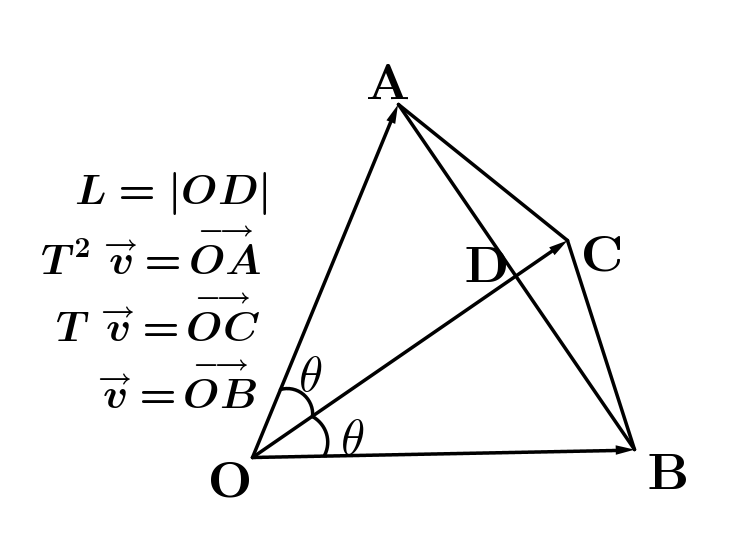
\includegraphics[scale=0.22]{./diagram.png}\par\vspace{-70pt}\quad
\hspace{180pt}{$\MathLeftMid{l}{Tv=\displaystyle\frac{\left|\overset{\rightarrow}{v}\right|}{2L}\Par{T^2 v+v}\Rightarrow T=\frac{\left|\overset{\rightarrow}{v}\right|}{2L}\Par{T^2+I}\\\vspace{8pt}\displaystyle L=\left|\overset{\rightarrow}{v}\right|\cos\theta\Rightarrow\frac{\left|\overset{\rightarrow}{v}\right|}{2L}=\frac{1}{2\cos\theta}}$}\par\vspace{8pt}\quad
Hence $p\Par{T}=T^2-2\cos\theta\, T+I=0$ and $z^2-2\cos\theta\, z+1$ is the mini poly of $T.$\PfEnd\vspace{3pt}\quad
\Or By (4E 5.B.11), $\Mt[\BigPar]{T,\Par{e_1,e_2}}=
\begin{pmatrix}
	\Blind{-}\cos\theta & \sin\theta\\
	-\sin\theta & \cos\theta
\end{pmatrix}.$\par\quad
Hence the mini poly is $z\pm 1$ or $z^2-2\cos\theta\,z+1.$\PfEnd
\SepLine

\ProblemBnoor{4E 5.B.11}{
	\TextB{Suppose $V$ is a two-dim vecsp, $T\in\Lm{V}$, and the matrix of $T$}
	\TextB{with resp to some basis of \,$V$ is {\large$\begin{pmatrix} a & c\\ b & d\end{pmatrix}.$}}
	(a) \TextB{Show that $T^2 - \Par{a + d}T + \Par{ad - bc}I = 0.$}
	(b) \TextB{Show that the mini poly of $T$ equals}
	\TextB{\large\envFontDefault\centerline{$\MathLeftBrace{l}{z-a\qquad\qquad\qquad\qquad\qquad$ if $b=c=0$ and $a=d$,$\\ z^2-\Par{a+d}z+\Par{ad-bc}\quad$ \,\,otherwise.$}$}}
}
\par

(a) Suppose the basis is $\Par{v,w}$. Because $\MathLeftBrace{l}{\displaystyle Tv=av+bw\Rightarrow \Par{T-aI}v=bw,$ then apply $\Par{T-dI}$ to both sides. $\\ Tw=cv+dw\Rightarrow \Par{T-dI}w=cv,$ then apply $\Par{T-aI}$ to both sides. $}$\par\vspace{6pt}\quad\Ha
Hence $\Par{T-aI}\Par{T-dI}=bc I\Rightarrow T^2 - \Par{a + d}T + \Par{ad - bc}I = 0.$\par\quad
(b) If $b=c=0$ and $a=d.$ Then $\Mt{T}=${\small$\begin{pmatrix}a & 0\\ 0 & a\end{pmatrix}$}$=a\Mt{I}$. Thus $T=aI.$ Hence the mini poly is $z-a.$\par\quad\Hb
Otherwise, by (a), $z^2-\Par{a+d}z+\Par{ad-bc}$ is a poly multi of the mini poly.\par\quad\Hb
Now we prove that $T\not\in\Span{I},$ so that then the mini poly of $T$ has exactly degree $2.$\par\quad\Hb
( At least one of the assumption of (I),(II) below is true. )\par\quad\Hb
(I) Suppose $a=d,$ then $Tv=av+bw\not\in\Span{v},Tw=cv+aw\not\in\Span{w}.$\par\qquad
(II) Suppose at most one of $b,c$ is not $0.$ If $b=0,$ then $Tw\not\in\Span{w};$ If $c=0,$ then $Tv\not\in\Span{v}.$\PfEnd
\SepLine

\ProblemN{5}{
	\TextN{Suppose $S,T\in\Lm{V},S$ is inv, and $p\in\PoF{}$. Prove that $p\Par{TS} = S^{-1} p\Par{ST}S.$}
}\par\quad
We prove $\Par{TS}^m=S^{-1}\Par{ST}^m S$ for each $m\in\Nbb\,$ by induction.\par\quad
(i) $m=0,1.$ $TS^0=I=S^{-1}\Par{ST}^0S;\,\,\,TS=S^{-1}\Par{ST}S.$\par\quad\Endi
(ii) $m>1.$ Assume that $\Par{TS}^m=S^{-1}\Par{ST}^m S.$\par\quad\Hii\qquad\quad\hspace{-1.5pt}
Then $\Par{TS}^{m+1}=\Par{TS}^m\Par{TS}=S^{-1}\Par{ST}^m STS=S^{-1}\Par{ST}^{m+1} S.$\par\quad
Hence $\forall p\in\PoF{},$\vspace{-23.5pt}\par\quad
\AlignEq{}{\quad p(TS)&=a_0 (TS)^0+a_1 (TS)+\dots+a_m (TS)^m\\&=a_0 [S^{-1}(ST)^0 S]+a_1 [S^{-1}(ST)S]+\dots+a_m [S^{-1}(ST)^m S]\\&=S^{-1}[a_0 (ST)^0+a_1 (ST)+\dots+a_m (ST)^m]S\\&=S^{-1}p(ST)S.}\PfEnd
\SepLine

\ProblemBnoor{4E 5.B.7}{
	\TextB{}
	(a) \TextB{Give an example of $S, T\in\Lm{\Fbb^2}$ such that}
	\Ha\TextB{the mini poly of
$ST$ does not equal the mini poly of $TS$.}
	(b) \TextB{Suppose $V$ is finite-dim and $S, T\in\Lm{V}$. Prove that if $S$ or $T$ is inv,}
	\Hb\TextB{then the mini poly of $ST$ equals the mini poly of $TS$.}
}\par\quad
(a) %Let $V=\Fbb^{\infty},$ $S\in\Lm{\Fbb^\infty}$ is the forward shift operator, $T\in\Lm{\Fbb^\infty}$ is the backward shift operator.\par\quad\Ha
%Then $ST(x_1,x_2,x_3,\dots)=(0,x_2,x_3,\dots)\Rightarrow 0,1$ are all the eigvals of $ST,$ $(ST)^2-(ST)=0.$\par\quad\Ha
%$TS(x_1,x_2,\dots)=(x_1,x_2,\dots)\Rightarrow 1$ is the only eigval of $TS,$ $TS=I.$\par\quad\Ha
Define $S$ by $S\Par{x,y}=\Par{x,x}.$ Define $T$ by $T\Par{x,y}=\Par{0,y}.$\par\quad\Ha
Then $ST\Par{x,y}=0,\,\,TS\Par{x,y}=\Par{0,x}$ for all $\Par{x,y}\in\Fbb^2.$\par\quad\Ha
Thus $ST=0\neq TS$ and $\Par{TS}^2=0.$\par\quad\Ha
Hence the mini poly of $ST$ does not equal to the mini poly of $TS.$\par\quad
(b) Denote the mini poly of $ST$ by $p,$ and the mini poly $TS$ by $q.$\par\quad\Hb
Suppose $S$ is inv.\par\,\,\Hb
$\MathRightBrace{l}{$
$p\Par{ST}=0=S p\Par{TS}S^{-1}\Rightarrow p\Par{TS}=0,p$ is a poly multi of $q.\\ $
$q\Par{TS}=0=S^{-1} q\Par{ST}S\Rightarrow q\Par{ST}=0,q$ is a poly multi of $p.$
$}\Rightarrow p=q.$\par\vspace{6pt}\quad\Hb
Reversing the roles of $S$ and $T$, we conclude that if $T$ is inv, then $p=q$ as well.\PfEnd
\SepLine

\ProblemN{11}{
	\TextNL{Suppose $\Fbb = \Cbb,$ $T\in\Lm{V}, p\in\PoC{}$, and $\alpha\in\Cbb.$}
	\TextNL{Prove that $\alpha$ is an eigval of $p\Par{T}$ $\Longleftrightarrow$ $\alpha = p\Par{\lambda}$ for some eigval $\lambda$ of $T$.}
}\par\quad
(a) Suppose $\alpha$ is an eigval of $p\Par{T}\Leftrightarrow \BigPar{p\Par{T}-\alpha I}$ is not inje.\par\quad\Ha
Write $p\Par{z}-\alpha=c\Par{z-\lambda_1}\cdots\Par{z-\lambda_m}\Rightarrow p\Par{T}-\alpha I=c\Par{T-\lambda_1 I}\cdots\Par{T-\lambda_m I}.$\par\quad\Ha
By \TIPS, $\exists\,\Par{T-\lambda_j I}$ not inje. Thus $p\Par{\lambda_j}-\alpha=0.$\par\quad
(b) Suppose $\alpha=p\Par{\lambda}$ and $\lambda$ is an eigval of $T$ with an eigvec $v.$ Then $p\Par{T}v=p\Par{\lambda}v=\alpha v.$\PfEnd\vspace{3pt}\quad\Hb
\Or Define $q$ by $q\Par{z}=p\Par{z}-\alpha.$ $\lambda$ is a zero of $q.$\par\quad\Hb
Because $q\Par{T}v=\BigPar{p\Par{T}-\alpha I}v=q\Par{\lambda}v=\BigPar{p\Par{\lambda}-\alpha}v=0.$\par\quad\Hb
Hence $q\Par{T}$ is not inje $\Rightarrow \BigPar{p\Par{T}-\alpha I}$ is not inje.\PfEnd
\SepLine

\ProblemNor{12}{4E.5.B.6}{
	\TextNL{Give an example of an operator on $\Rbb^2$}
	\TextNL{that shows the result above does not hold if $\Cbb$ is replaced with $\Rbb$.}
}\par\quad
Define $T\in\Lm{\Rbb^2}$ by $T\Par{w,z}=\Par{-z,w}.$\par\quad
By Problem (4E 5.B.11), $\Mt[\BigPar]{T,\Par{\Par{1,0},\Par{0,1}}}=\,${\small$\begin{pmatrix}0 & -1\\ 1 & 0\end{pmatrix}$}$\Rightarrow$ the mini poly of $T$ is $z^2+1.$\par\quad
Define $p$ by $p\Par{z}=z^2.$ Then $p\Par{T}=T^2=-I.$ Thus $p\Par{T}$ has eigval $-1.$\par\quad
While $\nexists\,\lambda\in\Rbb$ such that $-1=p\Par{\lambda}=\lambda^2.$\PfEnd
\SepLine

\ProblemBnoor{4E 5.B.17}{
	\TextB{Suppose $V$ is finite-dim, $T\in \Lm{V},\lambda\in\Fbb$, and $\,p\,$ is the mini poly of $T$.}
	\TextB{Show that the mini poly of $\Par{T - \lambda I}$ is the poly $q$ defined by $q\Par{z} = p\Par{z + \lambda}.$}
}\par\quad
$q\Par{T-\lambda I}=0\Rightarrow q$ is poly multi of the mini poly of $\Par{T-\lambda I}.$\par\quad
Suppose the degree of the mini poly of $\Par{T-\lambda I}$ is $n,$ and the degree of the mini poly of $T$ is $m.$\par\quad
%Write $q(z)=p(z+\lambda)=a_0+a_1(z+\lambda)+\dots+a_{m-1}(z+\lambda)^{m-1}+(z+\lambda)^m.$\par\quad
By definition of mini poly,\par\quad
$n$ is the smallest such that $\Par{T-\lambda I}^n\in\Span{I,\Par{T-\lambda I},\dots,\Par{T-\lambda I}^{n-1}};$\par\quad
$m$ is the smallest such that $T^m\in\Span{I,T,\dots,T^{m-1}}.$\par\quad
又 $T^k\in\Span{I,T,\dots,T^{k-1}}\Longleftrightarrow \Par{T-\lambda}^k\in\Span{I,\Par{T-\lambda I},\dots,\Par{T-\lambda I}^{k-1}}.$\par\quad
Thus $n=m.$ 又 $q$ is monic. By the uniqnes of mini poly.\PfEnd
\SepLine

\ProblemBnoor{4E 5.B.18}{
	\TextB{Suppose $V$ is finite-dim, $T\in \Lm{V},\lambda\in\Fbb\backslash\zeroSubs$, and $\,p\,$ is the mini poly of $T$.}
	\TextB{Show that the mini poly of $\lambda T$ is the poly q defined by $q\Par{z} = \lambda^{\deg p} p\Par{\frac{z}{\lambda}}$.}
}\par\quad
$q\Par{\lambda T}=\lambda^{\deg p}p\Par{T}=0\Rightarrow q$ is a poly multi of the mini poly of $\lambda T.$\par\quad
Suppose the degree of the mini poly of $\lambda T$ is $n,$ and the degree of the mini poly of $T$ is $m.$\par\quad
By definition of mini poly,\par\quad
$n$ is the smallest such that $\Par{\lambda T}^n\in\Span{\lambda I,\lambda T,\dots,\Par{\lambda T}^{n-1}};$\par\quad
$m$ is the smallest such that $T^m\in\Span{I,T,\dots,T^{m-1}}.$\par\quad
又 $\Par{\lambda T}^k\in\Span{\lambda I,\lambda T,\dots,\Par{\lambda T}^{k-1}}\Longleftrightarrow T^k\in\Span{I,T\dots,T^{k-1}}.$\par\quad
Thus $n=m.$ 又 $q$ is monic. By the uniqnes of mini poly.\PfEnd
\SepLine

\ProblemNor{18}{4E 5.B.15}{
	\TextNL{Suppose $V$ is a finite-dim complex vecsp with $\dim V > 0$ and $T\in\Lm{V}$.}
	\TextNL{Define $f:\Cbb\rightarrow\Rbb$ by $f\Par{\lambda} = \dim \range\Par{T-\lambda I}$.}
	\TextNL{Prove that $f$ is not a continuous function.}
}Note that $V$ is finite-dim.\par\quad
Let $\lambda_0$ be an eigval of $T.$ Then $\Par{T-\lambda_0 I}$ is not surj. Hence $\dim\range\Par{T-\lambda_0 I}<\dim V.$\par\quad
Because $T$ has finitely many eigvals. There exist a sequence of number $\Bra{\lambda_n}$ such that $\lim\limits_{n\rightarrow\infty}\lambda_n=\lambda_0$.\par\quad
And $\lambda_n$ is not an eigval of $T$ for each $n\Rightarrow\dim\range\Par{T-\lambda_n I}=\dim V\neq \dim\range\Par{T-\lambda_0 I}.$\par\quad
Thus $f\Par{\lambda_0}\neq \lim\limits_{n\rightarrow\infty}f\Par{\lambda_n}.$\PfEnd
\SepLine

\ProblemBnoor{4E 5.B.9}{
	\TextB{Suppose $T\in\Lm{V}$ is such that with resp to some basis of \,$V$,}
	\TextB{all entries of the matrix of $T$ are rational numbers.}
	\TextB{Explain why all coefficients of the mini poly of $T$ are rational numbers.}
}\par\quad
Let $\Par{v_1,\dots,v_n}$ denote the basis such that $\Mt[\BigPar]{T,\Par{v_1,\dots,v_n}}_{j,k}=A_{j,k}\in\Qbb$ for all $j,k=1,\dots,n$.\par\quad
Denote $\Mt[\BigPar]{v_j,\Par{v_1,\dots,v_n}}$ by $x_j$ for each $v_j.$\par\quad
Suppose $p$ is the mini poly of $T$ and $p\Par{z}=z^m+\dots+c_1 z+c_0.$ Now we show that each $c_j\in\Qbb.$\par\quad
Note that $\forall s\in\Nbp,\Mt{T^s}=\Mt{T}^s=A^s\in\Qbb^{n,n}$ and $T^s v_k=A^s_{1,k} v_1+\dots+A^s_{n,k}v_n$ for all $k\in\Bra{1,\dots,n}.$\par\vspace{6pt}\quad
Thus $\MathLeftBrace{l}{
\Mt{p\Par{T}v_1}=\Par{A^m+\dots+c_1 A+c_0 I}x_1=\sum\limits_{j=1}^n\Par{A^m+\dots+c_1 A+c_0 I}_{j,1}x_j=0;\\ \qquad\qquad\vdots \\
\Mt{p\Par{T}v_n}=\Par{A^m+\dots+c_1 A+c_0 I}x_n=\sum\limits_{j=1}^n\Par{A^m+\dots+c_1 A+c_0 I}_{j,n}x_j=0;
}$\par\quad
More clearly, $\MathLeftBrace{l}{
\Par{A^m+\dots+c_1 A+c_0 I}_{1,1}=\cdots=\Par{A^m+\dots+c_1 A+c_0 I}_{n,1}=0;\\\hspace{130pt}\vdots\hspace{8pt}\ddots\hspace{8pt}\vdots\\
\Par{A^m+\dots+c_1 A+c_0 I}_{1,n}=\cdots=\Par{A^m+\dots+c_1 A+c_0 I}_{n,n}=0;
}$\par\quad
Hence we get a system of $n^2$ linear equations in $m$ unknowns $c_0,c_1,\dots,c_{m-1}.$\par\quad
We conclude that $c_0,c_1,\dots,c_{m-1}\in\Qbb.$\PfEnd
\SepLine

\ProblemBnoor{\OR (4E 5.B.16), \OR (8.C.18)}[\Sbra]{
	\TextB{Suppose $a_0 ,\dots, a_{n-1}\in\Fbb.$ Let $T$ be the operator on $\Fbb^n$ such that\vspace{2pt}}
	\TextB{$\Mt{T}=\,${\normalsize$\begin{pmatrix}
	0 &   &        &  &   & -a_0     \\
	1 & 0 &        &  &   & -a_1     \\
	  & 1 & \ddots &  &   & \vdots   \\
	  &   & \ddots &  & 0 & -a_{n-2} \\
	0 &   &        &  & 1 & -a_{n-1}
\end{pmatrix} $}, with resp to the standard basis $\Par{e_1,\dots,e_n}$.\vspace{4pt}}
	\TextB{Show that the mini poly of $T$ is $\,p\,$ defined by $p\Par{z}=a_0 + a_1 z + \dots + a_{n-1} z^{n-1} + z^n$.}
	\vspace{-2pt}\TextB{\small $\Mt{T}$ is called the {\tgsc companion matrix} of the poly above. This exercise shows that every monic poly is the mini poly of some operator.}
	\vspace{-2pt}\TextB{\small Hence a formula or an algorithm that could produce exact eigvals for each operator on each $\Fbb^n$ could then produce exact zeros for}
	\vspace{-2pt}\TextB{\small each poly  $[$ by 8.36(b) $]$. Thus there is no such formula or algorithm. However, efficient numeric methods exist for obtaining very good}
	\TextB{\small approximations for the eigvals of an operator.}
}Note that $\Par{e_1,Te_1,\dots,T^{n-1}e_1}$ is linely inde. 又 The deg of mini poly is at most $n.$\par\quad
$T^n e_1=\cdots=T^{n-k}e_{1+k}=\cdots=T e_n=-a_0 e_1-a_1 e_2-a_2 e_3-\dots-a_{n-1}e_n$\par
$=\Par{-a_0 I-a_1 T-a_2 T^2-\dots-a_{n-1}T^{n-1}}e_1.$ Thus $p\Par{T}e_1=0=p\Par{T}e_j$ for each $e_j=T^{j-1}e_1.$\PfEnd
\SepLine

\BulletPoint \,\hspace{1pt}{\Large\textsc{Eigenvalues On Odd-Dimensional Real Vector Spaces}}\par
\ProblemB{
	\textsc{Even-Dimensional Null Space}\TextB{}
	\TextB{Suppose $\Fbb=\Rbb,$ $V$ is finite-dim, $T\in\Lm{V}$ and $b, c\in\Rbb$ with $b^2 < 4c$.}
	\TextB{Prove that $\dim\null\Par{T^2 + bT + cI}$ is an even number.}
}\par\quad
Denote $\null\Par{T^2 + bT + cI}$ by $R.$ Then $T\mid_R+bT\mid_R+cI_R=\Par{T+bT+cI}\mid_R=0\in\Lm{R}.$\par\quad
Suppose $\lambda$ is an eigval of $T_R$ with an eigvec $v\in R.$\par\quad
Then $\displaystyle 0=\Par{T\mid_R^2+bT\mid_R+cI_R}\Par{v}=\Par{\lambda^2+\lambda b+c}v=\BigPar{\Par{\lambda+b}^2+c-\frac{b^2}{4}}v.$\par\quad
Because $\displaystyle c-\frac{b^2}{4}>0$ and we have $v=0.$ Thus $T_R$ has no eigvals.\par\quad
Let $U$ be an invar subsp of $R$ that has the largest, even dim among all invar subsps.\par\quad
Assume that $U\neq R.$ Then $\exists\,w\in R$ but $w\not\in U.$ Let $W$ be such that $\Par{w,T\mid_R w}$ is a basis of $W.$\par\quad
Because $T\mid_R^2 w=-bT\mid_R w-cw\in W.$ Hence $W$ is an invar subsp of dim $2.$\par\quad
Thus $\dim \Par{U+W}=\dim U+2-\Dim\Par{U\cap W},$ where $U\cap W=\zeroSubs,$\par\qquad\qquad
for if not, because $w\not\in U,T\mid_R w\in U,$\par\qquad\qquad $U\cap W$ is invar under $T\mid_R$ of one dim ( impossible because $T\mid_R$ has no eigvecs ).\par\quad
Hence $U+W$ is even-dim invar subsp under $T\mid_R$, contradicting the maximality of $\dim U.$\par\quad
Thus the assumption was incorrect. Hence $R=\null\Par{T^2+bT+cI}=U$ has even dim.\PfEnd
\SepLine

\ProblemB{
	\textsc{Operators On Odd-Dimensional Vector Spaces Have Eigenvalues}\TextB{}
	(a) \TextB{Suppose $\Fbb=\Cbb.$ \tgnr\large Then by [5.21], we are done.}
	(b) \TextB{Suppose $\Fbb=\Rbb,$ $V$ is finite-dim, and $\dim V=n$ is an odd number.}
	\Hb\TextB{Let $T\in\Lm{V}$ and the mini poly is $\,p\,$. Prove that $T$ has an eigval.}
}\par\quad
(i) If $n=1,$ then we are done.\par\quad\Endi
(ii) Suppose $n\geqslant 3.$ Assume that every operator, on odd-dim vecsps of dim less than $n,$ has an eigval.\par\quad\Hii
If $p$ is a poly multi of $\Par{x - \lambda}$ for some $\lambda\in\Rbb,$ then by [8.49] $\lambda$ is an eigval of $T$ and we are done.\par\quad\Hii
Now suppose $b, c\in\Rbb$ such that $b^2 < 4c$ and $p$ is a poly multi of $x^2 + bx + c$ (see [4.17]).\par\quad\Hii
Then $\exists\,q\in\PoR{}$ such that $p\Par{x} = q\Par{x}\Par{x^2 + bx + c}$ for all $x\in\Rbb.$\par\quad\Hii
Now $0 = p\Par{T} = \BigPar{q\Par{T}}\Par{T^2 + bT + cI},$ which means that $q\Par{T}\mid_{\range\Par{T^2+bT+cI}}=0.$\par\quad\Hii
Because $\deg q < \deg p$ and $p$ is the mini poly of $T$, hence $\range\Par{T^2 + bT + cI}\neq V$.\par\quad\Hii
又 $\dim V$ is odd and $\dim\null\Par{T^2 +bT+cI}$ is even ( by our previous result ).\par\quad\Hii
Thus $\dim V - \dim \null\Par{T^2 + bT + cI}=\dim \range\Par{T^2 + bT + cI}$ is odd.\par\quad\Hii
By [5.18], $\range\Par{T^2 + bT + cI}$ is an invar subsp of $V$ under $T$ that has odd dim less than $n.$\par\quad\Hii
Our induction hypothesis now implies that $T\mid_{\range\Par{T^2 + bT + cI}}$ has an eigval.\par\quad
By mathematical induction.\PfEnd
\SepLine

\ProblemBnoor{2E Ch5.24}{
	\TextB{Suppose $\Fbb=\Rbb,T\in\Lm{V}$ has no eigvals.} \TextB{Prove that every invar subsp of \,$V$ under $T$ is even-dim.}
}\par\quad
Suppose $U$ is such a subsp. Then $T\mid_U\in\Lm{U}.$
We prove by contradiction.\par\quad
If $\dim U$ is odd, then $T\mid_U$ has an eigval and so is $T,$ so that $\exists$ invar subsp of $1$ dim, contradicts.\PfEnd
\SepLine

\ProblemBnoor{4E 5.B.29}{
	\TextB{Show that every operator on a finite-dim vecsp of dim $\geq 2$ has a $2$-dim invar subsp.}
}\par\quad
Using induction on $\dim V.$\par\quad
(i) $\dim V=2,$ we are done.\par\quad\Endi
(ii) $\dim V>2.$ Assume that the desired result is true for vecsp of smaller dim.\par\quad\Hii
Suppose $p$ is the mini poly of degree $m$ and $p\Par{z}=\Par{z-\lambda_1}\cdots\Par{z-\lambda_m}.$\par\quad\Hii
If $\,T=\lambda I\,\Par{\,\Leftrightarrow m=1\,\vee\,m=-\infty\,},$ then we are done. ( $m\neq 0$ because $\dim V\neq 0.$ )\par\quad\Hii
Now define a $q$ by $q\Par{z}=\Par{z-\lambda_1}\Par{z-\lambda_2}$.\par\quad\Hii
By assumption, $T\mid_{\null q\Par{T}}$ has an invar subsp of dim $2.$\PfEnd
\SepLine

\ChEnd

% 6h
\ChDecl{Ch5BII}{5.B: II}{}

\ProblemBnoor{4E 5.C.1}{
	\TextB{Prove or give a counterexample:}
	\TextB{If $T\in \Lm{V}$ and $T^2$ has an upper-trig matrix, then $T$ has an upper-trig matrix.}
}\par
\SepLine

\ProblemBnoor{4E 5.C.2}{
	\TextB{Suppose $A$ and $B$ are upper-trig matrices of the same size,}
	\TextB{with $\alpha_1 , \dots , \alpha_n$ on the diag of $A$ and $\beta_1 , \dots , \beta_n$ on the diag of $B$.}
	(a) \TextB{Show that $A + B$ is an upper-trig matrix with $\alpha_1 + \beta_1 , \dots , \alpha_n + \beta_n$ on the diag.}
	(b) \TextB{Show that $AB$ is an upper-trig matrix with $\alpha_1 \beta_1 , \dots , \alpha_n \beta_n$ on the diag.}
}\par
\SepLine

\ProblemBnoor{4E 5.C.3}{
	\TextB{}
	\TextB{Suppose $T\in \Lm{V}$ is inv and $B=\Par{v_1 , \dots , v_n}$ is a basis of \,$V$ such that}
	\TextB{$\Mt{T,B}=A$ is upper trig, with $\lambda_1 , \dots , \lambda_n$ on the diag.}
	\TextB{Show that the matrix of $\Mt{T^{-1},B}=A^{-1}$ is also upper trig, with
{\normalsize$\displaystyle\frac{1}{\lambda_1},\dots,\frac{1}{\lambda_n}$} on the diag.}
}\par
\SepLine

\ProblemNnoor{9}{4E 5.C.7}{
	\TextN{}
	\TextN{Suppose $V$ is finite-dim, $T\in \Lm{V}$, and $v \in V$.}
	(a) \TextN{Prove that $\exists\,!$ monic poly $p_v$ of smallest degree such that $p_v \Par{T}v = 0$.}
	(b) \TextN{Prove that the mini poly of $T$ is a poly multi of $p_v$.}
}\par
\SepLine


\ProblemNor{14}{4E 5.C.4}{
	\TextNL{ Give an operator $T$ such that with resp to some basis,}
	\TextNL{$\Mt{T}_{k,k}=0$ for each $k$, while $T$ is inv.}
}
\par
\SepLine

\ProblemNor{15}{4E 5.C.5}{
	\TextNL{Give an operator $T$ such that with resp to some basis,}
	\TextNL{$\Mt{T}_{k,k}\neq 0$ for each $k$, while $T$ is not inv.}
}\par


\par
\SepLine

\ProblemN{20}{
	({\normalsize \OR 4E 5.C.6})\TextNL{}
	\TextNL{Suppose $\Fbb=\Cbb,$ $V$ is finite-dim, and $T\in\Lm{V}$.}
	\TextNL{Prove that if $k\in\Bra{1,\dots,\dim V},$ then \,$V$ has a $k$ dim subsp invar under $T$.}
}\par
\SepLine

\ProblemBnoor{4E 5.C.8}{
	\TextB{Suppose $V$ is finite-dim, $T\in \Lm{V}$, and $\exists\,v \in V\backslash\zeroSubs$ such that $T^2 v + 2Tv = -2v$.}
	(a) \TextB{Prove that if $\Fbb=\Rbb,$ then $\nexists$ a basis of \,$V$ with resp to which $T$ has an upper-trig matrix.}
	(b) \TextB{Prove that if $\Fbb=\Cbb$ and $A$ is an upper-trig matrix that equals the matrix of $T$}
	\Hb\TextB{with resp to some basis of \,$V$, then $-1 + \i$ or $-1 - \i$ appears on the diag of $A$.}
}\par
\SepLine

\ProblemBnoor{4E 5.C.9}{
	\TextB{Suppose $B\in\Fbb^{n,n}$ with complex entries.}
	\TextB{Prove that $\exists$ inv $A\in\Fbb^{n,n}$ with complex entries such that $A^{-1} BA$ is an upper-trig matrix.}
}\par

\par
\SepLine

\ProblemBnoor{4E 5.C.10}{
	\TextB{Suppose $T\in \Lm{V}$ and $\Par{v_1,\dots,v_n}$ is a basis of \,$V$.}
	\TextB{Show that the following are equi.}
	(a) \TextB{The matrix of $T$ with resp to $\Par{v_1,\dots,v_n}$ is lower trig.}
	(b) \TextB{$\Span{v_k,\dots,v_n}$ is invar under $T$ for each $k=1,\dots,n$.}
	(c) \TextB{$Tv_k\in\Span{v_k,\dots,v_n}$ for each $k=1,\dots,n$.}
}\par
\SepLine

\ProblemBnoor{4E 5.C.11}{
	\TextB{Suppose $\Fbb=\Cbb$ and $V$ is finite-dim.}
	\TextB{Prove that if $T\in \Lm{V}$, then $T$ has a lower-trig matrix with resp to some basis.}
}\par
\SepLine

\ProblemBnoor{4E 5.C.12}{
	\TextB{}
	\TextB{Suppose $V$ is finite-dim, $T\in \Lm{V}$ has an upper-trig matrix with resp to some basis,}
	\TextB{and $U$ is a subsp of \,$V$ that is invar under $T$.}
	(a) \TextB{Prove that $T\mid_U$ has an upper-trig matrix with resp to some basis of $U$.}
	(b) \TextB{Prove that $T/U$ has an upper-trig matrix with resp to some basis of \,$V/U$.}
}\par


\par
\SepLine

\ProblemBnoor{4E 5.C.13}{
	\TextB{Suppose $V$ is finite-dim, $T\in \Lm{V}$. Suppose $U$ is an invar subsp of \,$V$ under $T$}
	\TextB{such that $T\mid_U$ has an upper-trig matrix and also $T/U$ has an upper-trig matrix.}
	\TextB{Prove that $T$ has an upper-trig matrix.}
}\par


\par
\SepLine

\ProblemBnoor{4E 5.C.14}{
	\TextB{Suppose $V$ is finite-dim and $T\in \Lm{V}$.}
	\TextB{Prove that $T$ has an upper-trig matrix $\Longleftrightarrow$ $T\apostrophe$ has an upper-trig matrix.}
}\par


\par
\SepLine

\ChEnd

\ChDecl{Ch5C}{5.C} % 10h

XXXX


\par
\SepLine

\ChEnd
\ChDecl{Ch5E}{5.E* (4E)} % 0.5h/4h

\ProblemN{1}{
	\TextN{Give an example of two commuting operators $S, T\in\Fbb^4$ such that}
	\TextN{there is an invar subsp of $\Fbb^4$ under $S$ but not under $T$}
	\TextN{and an invar subsp of $\Fbb^4$ under $T$ but not under $S$.}
}
\par
\SepLine

\ProblemN{2}{
	\TextN{Suppose $\mathcal{E}$ is a subset of $\Lm{V}$ and every element of $\mathcal{E}$ is diagable.}
	\TextN{Prove that $\exists$ a basis of \,$V$ with resp to which}
	\TextN{every element of $\mathcal{E}$ has a diag matrix $\Longleftrightarrow$ every pair of elements of $\mathcal{E}$ commutes.}
	\TextN{{\normalsize This exercise extends [5.76], which considers the case in which $\mathcal{E}$ contains only two elements.}}\hspace{0.5pt}
	\TextN{{\normalsize For this exercise, $\mathcal{E}$ may contain any number of elements, and $\mathcal{E}$ may even be an infinite set.}}
}\par
\SepLine

\ProblemN{3}{
	\TextN{Suppose $S, T\in\Lm{V}$ are such that $ST = TS$. Suppose $p\in\PoF{}$.}
	(a) \TextN{Prove that $\null p\Par{S}$ is invar under $T$.}
	(b) \TextN{Prove that $\range p\Par{S}$ is invar under $T$.}
	\TextN{See \NOTEFOR [5.17] for the special case $S = T$.}
}\par
\SepLine

\ProblemN{4}{
	\TextN{Prove or give a counterexample:}
	\TextN{A diag matrix $A$ and an upper-trig matrix $B$ of the same size commute.}
}\par
\SepLine

\ProblemN{5}{
	\TextN{Prove that a pair of operators on a finite-dim vecsp commute $\Longleftrightarrow$ their dual operators commute.}
}\par
\SepLine

\ProblemN{6}{
	\TextN{Suppose $V$ is a finite-dim complex vecsp and $S, T\in\Lm{V}$ commute.}
	\TextN{Prove that $\exists\,\alpha,\lambda\in\Cbb$ such that $\range\Par{S -\alpha I} + \range\Par{T -\lambda I}\neq V$.}
}\par
\SepLine

\ProblemN{7}{
	\TextN{Suppose $V$ is a complex vecsp, $S\in\Lm{V}$ is diagable, and $T$ commutes with $S$.}
	\TextN{Prove that $\exists$ basis $B$ of $V$ such that $S$ has a diag matrix with resp to $B$}
	\TextN{and T has an upper-trig matrix with resp to $B$.}
}\par
\SepLine

\ProblemN{8}{
	\TextN{Suppose $m = 3$ in Example [5.72]}
	\TextN{and $D_x , D_y$ are the commuting partial differentiation operators on $\Po_3\Par{\Rbb^2}$ from that example.}
	\TextN{Find a basis of $\Po_3\Par{\Rbb^2}$ with resp to which $D_x$ and $D_y$ each have an upper-trig matrix.}
}\par
\SepLine

\ProblemN{9}{
	\TextN{Suppose $V$ is a finite-dim nonzero complex vecsp.}
	\TextN{Suppose that $\mathcal{E}\subseteq\Lm{V}$ is such that $S$ and $T$ commute for all $S, T\in\mathcal{E}$.}
	(a) \TextN{Prove that $\exists\,v\in V$ is an eigvec for every element of $\mathcal{E}$.}
	(b) \TextN{Prove that $\exists$ a basis of \,$V$ with resp to which every element of $\mathcal{E}$ has an upper-trig matrix.}
}\par
\SepLine

\ProblemN{10}{
	\TextNL{Give an example of two commuting operators $S, T$ on a finite-dim real vecsp such that}
	\TextNL{$S + T$ has a eigval that does not equal an eigval of $S$ plus an eigval of $T$}
	\TextNL{and $ST$ has a eigval that does not equal an eigval of $S$ times an eigval of $T$.}
}
\par
\SepLine
\ChEnd

\end{large}
\end{document}
